% =====================================================================
%  La Bibbia del Game Design -- volume autonomo: Fondamenti di Unreal Engine
%  Stesso contenuto della parte omonima del libro completo (main.tex).
% =====================================================================
\documentclass{book}
% Preambolo comune al libro completo (main.tex) e ai volumi autonomi (libro-*.tex).
\usepackage[margin=1in]{geometry}
%\usepackage[italian]{babel}, \usepackage[T1]{fontenc},
\usepackage[utf8]{inputenc} \usepackage{booktabs}
\usepackage{amsmath, amsfonts}
\usepackage{graphicx}
\usepackage{enumitem, url, siunitx, comment, booktabs}
\usepackage[colorlinks=true, linkcolor=blue]{hyperref}

\usepackage{amssymb, amsthm, algpseudocode}
\usepackage{bm}
\usepackage{mathtools}
\usepackage{tikz}
\usetikzlibrary{shapes.geometric,shapes.symbols,shapes.misc, arrows.meta,positioning,calc,fit}

\newtheorem{theorem}{Theorem}[chapter]
\newtheorem{definition}{Definition}[chapter]
\newtheorem{remark}{Remark}[chapter]
\newtheorem{example}{Example}[chapter]
\newtheorem{question}{Question}[chapter]


% Indice: spazio piu' largo per i numeri lunghi (es. 0.9.10, 2.1.10.3)
\usepackage{etoolbox}
\makeatletter
\patchcmd{\l@chapter}{1.5em}{2.4em}{}{}
\renewcommand*\l@section{\@dottedtocline{1}{1.5em}{3.3em}}
\renewcommand*\l@subsection{\@dottedtocline{2}{4.8em}{4.3em}}
\makeatother

% ---------------------------------------------------------------------
% Figure: le immagini tratte dalle slide e dalle dispense delle lezioni
% ---------------------------------------------------------------------
\usepackage{morefloats}
\extrafloats{150}
\setcounter{topnumber}{3}
\setcounter{bottomnumber}{2}
\setcounter{totalnumber}{5}
\renewcommand{\topfraction}{0.85}
\renewcommand{\bottomfraction}{0.6}
\renewcommand{\textfraction}{0.12}
\renewcommand{\floatpagefraction}{0.7}

% \slidefig{file}{didascalia}{fonte}{etichetta}
% Inserisce una slide (o un collage di slide) con didascalia e fonte.
\newcommand{\slidefig}[4]{%
  \begin{figure}[htbp]
    \centering
    \includegraphics[width=0.92\textwidth,height=0.42\textheight,keepaspectratio]{#1}
    \caption[#2]{#2 {\footnotesize\textit{(Fonte: #3.)}}}%
    \label{#4}
  \end{figure}}

% ---------------------------------------------------------------------
% Copertine dei volumi e delle parti
% ---------------------------------------------------------------------
% =====================================================================
%  copertine.tex -- copertine dei volumi e illustrazioni delle parti
% ---------------------------------------------------------------------
%  Uso:
%    \copertinaLibro{<chiave>}            copertina a tutta pagina di un volume
%    \parteillustrata{<chiave>}{<titolo>}  \part{<titolo>} con la pagina illustrata
%  Chiavi: completo, seminari, conferenze, unreal, agd, professioni,
%          gamedesign, revisioni.
%  Ogni copertina e' disegnata in TikZ (con alcune fotografie tratte dalle
%  slide delle lezioni per AGD e Game Design). La parte centrale resta
%  libera: nei volumi ospita titolo e autore, nel libro completo ospita il
%  titolo della parte stampato da \part.
% =====================================================================
\usetikzlibrary{shadows,decorations.pathmorphing,decorations.markings}

% --- Palette ----------------------------------------------------------
\definecolor{copNavy}{HTML}{0F1B33}
\definecolor{copGold}{HTML}{E8B84A}
\definecolor{copOrange}{HTML}{F08A24}
\definecolor{copRed}{HTML}{B5292E}
\definecolor{copPurple}{HTML}{241238}
\definecolor{copViolet}{HTML}{7B3FA0}
\definecolor{copBlueprint}{HTML}{1C2838}
\definecolor{copGridA}{HTML}{26364A}
\definecolor{copGridB}{HTML}{33485F}
\definecolor{copFelt}{HTML}{1E5C3C}
\definecolor{copFeltDark}{HTML}{123D27}
\definecolor{copTeal}{HTML}{0E4D55}
\definecolor{copTealLight}{HTML}{4FB3BF}
\definecolor{copSlate}{HTML}{22262E}
\definecolor{copCyan}{HTML}{3FC1E0}
\definecolor{copPaper}{HTML}{FBF8EF}
\definecolor{copRule}{HTML}{BFD3E6}
\definecolor{copPen}{HTML}{D0262B}
\definecolor{copPostit}{HTML}{FFE873}

% --- Elementi grafici riutilizzabili -----------------------------------
\tikzset{
  % dado a sei facce: faccia del 5
  dado5/.pic={
    \draw[pic actions, rounded corners=2.5pt, line width=0.6pt] (-.5,-.5) rectangle (.5,.5);
    \foreach \p in {(-.24,-.24),(.24,.24),(-.24,.24),(.24,-.24),(0,0)}
      \fill[black!85] \p circle (.085);
  },
  % dado a sei facce: faccia del 3
  dado3/.pic={
    \draw[pic actions, rounded corners=2.5pt, line width=0.6pt] (-.5,-.5) rectangle (.5,.5);
    \foreach \p in {(-.24,-.24),(.24,.24),(0,0)}
      \fill[black!85] \p circle (.085);
  },
  % meeple stilizzato
  meeple/.pic={
    \fill[pic actions] (0,.78) circle (.2);
    \fill[pic actions] (-.48,0) -- (-.14,0) -- (0,.24) -- (.14,0) -- (.48,0)
      -- (.22,.36) -- (.56,.5) to[out=90,in=0] (.3,.62) -- (-.3,.62)
      to[out=180,in=90] (-.56,.5) -- (-.22,.36) -- cycle;
  },
  % carta da gioco
  carta/.pic={
    \draw[pic actions, rounded corners=3pt, line width=0.6pt] (-.7,-1) rectangle (.7,1);
    \draw[rounded corners=2pt, line width=0.4pt, black!30] (-.55,-.85) rectangle (.55,.85);
  },
  % controller
  pad/.pic={
    \fill[pic actions, rounded corners=10pt] (-1.9,-.55) rectangle (1.9,.85);
    \fill[pic actions] (-1.45,-.45) circle (.8);
    \fill[pic actions] (1.45,-.45) circle (.8);
    \fill[copNavy] (-1.55,.05) rectangle (-1.05,.25);
    \fill[copNavy] (-1.4,-.1) rectangle (-1.2,.4);
    \foreach \p in {(1.3,.15),(1.55,.4),(1.55,-.1),(1.8,.15)}
      \fill[copNavy] \p circle (.1);
  },
  % cubo isometrico (blockout)
  cubo/.pic={
    \fill[pic actions, fill=black!55] (0,0) -- (.87,.5) -- (.87,1.5) -- (0,1) -- cycle;
    \fill[pic actions, fill=black!35] (0,0) -- (-.87,.5) -- (-.87,1.5) -- (0,1) -- cycle;
    \fill[pic actions, fill=black!15] (0,1) -- (.87,1.5) -- (0,2) -- (-.87,1.5) -- cycle;
  },
  % fumetto
  fumetto/.style={rounded corners=8pt, fill=white, fill opacity=.92, text opacity=1,
    inner xsep=10pt, inner ysep=7pt, font=\sffamily\bfseries},
  % fotografia con bordo bianco (polaroid)
  polaroid/.style={fill=white, inner sep=5pt, inner ysep=5pt, drop shadow={opacity=.45}},
}

% Nodo Blueprint: \copBPnode{x}{y}{larghezza}{colore}{titolo}{righe}
\newcommand{\copBPnode}[6]{%
  \begin{scope}[shift={(#1,#2)}]
    \fill[black, opacity=.35, rounded corners=4pt] (.12,-.12) rectangle ++(#3,-#6*0.55-.9);
    \fill[black!80, fill opacity=.92, rounded corners=4pt] (0,0) rectangle ++(#3,-#6*0.55-.9);
    \fill[#4, rounded corners=4pt] (0,0) rectangle ++(#3,-.7);
    \fill[#4] (0,-.4) rectangle ++(#3,-.3);
    \node[anchor=west, text=white, font=\sffamily\bfseries\small] at (.2,-.35) {#5};
    \foreach \r in {1,...,#6} {
      \fill[white!85!black] (.3,-.55-\r*0.55) circle (.09);
      \fill[white!30!black] (.55,-.6-\r*0.55) rectangle ++(1.3,.12);
    }
    \fill[white] (.15,-1.0) -- (.32,-1.0) -- (.42,-1.1) -- (.32,-1.2) -- (.15,-1.2) -- cycle;
    \fill[white] (#3-.45,-1.0) -- (#3-.28,-1.0) -- (#3-.18,-1.1) -- (#3-.28,-1.2) -- (#3-.45,-1.2) -- cycle;
  \end{scope}}

% --- Dati dei volumi -----------------------------------------------------
\makeatletter
\def\copertina@titolo@completo{La Bibbia del Game Design}
\def\copertina@sotto@completo{Lezioni, seminari e conferenze: il libro completo}
\def\copertina@vol@completo{Edizione completa}
\def\copertina@col@completo{copNavy}

\def\copertina@titolo@seminari{Seminari per il Game Designer}
\def\copertina@sotto@seminari{Feedback, leadership, Agile, producer, mindset, audio}
\def\copertina@vol@seminari{Volume 0}
\def\copertina@col@seminari{copRed}

\def\copertina@titolo@conferenze{Conferenze}
\def\copertina@sotto@conferenze{GAMM di Roma -- Checkpoint Festival \textperiodcentered\ On The Road, Zagarolo}
\def\copertina@vol@conferenze{Volume C}
\def\copertina@col@conferenze{copViolet}

\def\copertina@titolo@unreal{Fondamenti di Unreal Engine}
\def\copertina@sotto@unreal{Blueprint, materiali, animazione, luci e livelli}
\def\copertina@vol@unreal{Volume 1}
\def\copertina@col@unreal{copBlueprint}

\def\copertina@titolo@agd{Analog Game Design}
\def\copertina@sotto@agd{Giochi da tavolo, di ruolo, LARP e giochi pervasivi}
\def\copertina@vol@agd{Volume 2}
\def\copertina@col@agd{copFeltDark}

\def\copertina@titolo@professioni{Alcune Professioni nel Mondo Videoludico}
\def\copertina@sotto@professioni{Game, level e narrative design, animazione, programmazione, 3D art}
\def\copertina@vol@professioni{Volume 3}
\def\copertina@col@professioni{copTeal}

\def\copertina@titolo@gamedesign{Game Design}
\def\copertina@sotto@gamedesign{Metodi di design, documentazione e level design}
\def\copertina@vol@gamedesign{Volume 4}
\def\copertina@col@gamedesign{copSlate}

\def\copertina@titolo@revisioni{Revisioni dei Compiti}
\def\copertina@sotto@revisioni{Gli errori ricorrenti nei task, e come evitarli}
\def\copertina@vol@revisioni{Volume 5}
\def\copertina@col@revisioni{copPen}

% --- Sfondi ---------------------------------------------------------------
% Ogni sfondo disegna in coordinate di pagina (cm), con \W e \H dimensioni
% del foglio. La fascia centrale (circa H/2 +- 4.6 cm) resta per i testi.

% Libro completo: tavolo da gioco notturno, analogico e digitale insieme
\def\copertina@completo{%
  \fill[copNavy] (0,0) rectangle (\W,\H);
  \begin{scope}[opacity=.13]
    \foreach \i in {0,...,14} \foreach \j in {0,...,20} {
      \pgfmathsetmacro{\hx}{\i*1.6 + mod(\j,2)*0.8}
      \pgfmathsetmacro{\hy}{\j*1.39}
      \node[draw=copGold, line width=.5pt, regular polygon, regular polygon sides=6,
            minimum size=1.6cm, inner sep=0pt] at (\hx,\hy) {};
    }
  \end{scope}
  % alone centrale
  \fill[copGold, opacity=.06] (\W/2,\H/2) circle (10);
  % icone in alto
  \pic[fill=copGold, rotate=-12, scale=1.6] at (3.4,\H-4.4) {dado5};
  \pic[fill=white, rotate=18, scale=1.1] at (5.4,\H-3.1) {dado3};
  \pic[fill=copGold, scale=1.15] at (\W-4,\H-4.6) {pad};
  \pic[fill=copRed, scale=1.3] at (\W/2-1.2,\H-5.2) {meeple};
  \pic[fill=copCyan, scale=1.3] at (\W/2+1.2,\H-5.2) {meeple};
  \pic[fill=white, rotate=-8] at (\W/2-3.6,\H-3) {carta};
  \pic[fill=copGold!30, rotate=6] at (\W/2+3.4,\H-2.8) {carta};
  % mini flowchart in basso
  \begin{scope}[shift={(2.2,4.6)}, every node/.style={font=\sffamily\scriptsize\bfseries, text=copNavy}]
    \node[fill=copGold, rounded corners=6pt, minimum width=1.6cm, minimum height=.7cm] (a) at (0,0) {START};
    \node[fill=white, minimum width=1.8cm, minimum height=.7cm] (b) at (3,0) {IDEA};
    \node[fill=copCyan, diamond, aspect=1.6, inner sep=1pt] (c) at (6.3,0) {PLAYTEST?};
    \node[fill=white, minimum width=1.8cm, minimum height=.7cm] (d) at (9.8,0) {ITERA};
    \node[fill=copGold, rounded corners=6pt, minimum width=1.6cm, minimum height=.7cm] (e) at (13.4,0) {GIOCO};
    \draw[-{Stealth[length=3mm]}, white, line width=1pt] (a) -- (b);
    \draw[-{Stealth[length=3mm]}, white, line width=1pt] (b) -- (c);
    \draw[-{Stealth[length=3mm]}, white, line width=1pt] (c) -- (d);
    \draw[-{Stealth[length=3mm]}, white, line width=1pt] (d) -- (e);
    \draw[-{Stealth[length=3mm]}, white, line width=1pt, dashed] (d.south) to[bend left=35] (b.south);
  \end{scope}
  % dorsi dei sette volumi
  \foreach \c/\t [count=\k] in {copRed/0, copViolet/C, copBlueprint/1, copFelt/2, copTeal/3, copSlate/4, copPen/5} {
    \pgfmathsetmacro{\sx}{\W/2 - 7*1.1/2 + (\k-1)*1.1}
    \fill[\c, draw=copGold, line width=.6pt] (\sx,1.2) rectangle ++(1,2.2);
    \node[text=copGold, font=\sffamily\bfseries] at (\sx+.5,2.3) {\t};
  }
}

% Seminari: un caldo dialogo di fumetti
\def\copertina@seminari{%
  \shade[top color=copOrange, bottom color=copRed] (0,0) rectangle (\W,\H);
  \foreach \x/\y/\r in {3/24/2.4, 18/22.5/3.2, 9/26/1.4, 19/5/2.6, 2.5/4/1.8, 11/2/1.1}
    \fill[white, opacity=.08] (\x,\y) circle (\r);
  \foreach \x/\y/\t/\a in {
      2.6/\H-2.6/Feedback/-6, 9.0/\H-2.0/Leadership/4, 15.6/\H-2.9/Agile e Scrum/-3,
      4.8/\H-5.3/Publisher/5, 11.3/\H-4.9/Producer/-4, 17.2/\H-5.9/Mindset/7,
      3.4/5.4/Hackerare un gioco/4, 11.0/6.0/Metaverso/-5, 17.0/4.8/Game audio/3,
      6.8/2.4/Tempo e idee/-3, 14.8/2.1/Cultura del feedback/2} {
    \node[fumetto, text=copRed, rotate=\a, font=\sffamily\bfseries\large] (f) at (\x,\y) {\t};
    \fill[white, opacity=.92, rotate around={\a:(f.center)}]
      ([xshift=-6pt]f.south) -- ([xshift=6pt]f.south) -- ([xshift=-14pt,yshift=-10pt]f.south) -- cycle;
  }
  % microfono
  \begin{scope}[shift={(\W-2.4,\H/2+5.4)}, rotate=-20]
    \fill[white, opacity=.9, rounded corners=8pt] (-.45,0) rectangle (.45,1.4);
    \fill[copRed!70!black] (-.12,-1.6) rectangle (.12,0);
    \draw[white, line width=1.5pt] (-.65,.6) to[out=-90,in=-90] (.65,.6);
  \end{scope}
}

% Conferenze: palco, riflettori e pubblico
\def\copertina@conferenze{%
  \fill[copPurple] (0,0) rectangle (\W,\H);
  % riflettori
  \foreach \x/\tx in {3/6, .5*\W/.5*\W, \W-3/\W-6} {
    \fill[white, opacity=.10] (\x,\H) -- (\tx-3.2,3.2) -- (\tx+3.2,3.2) -- cycle;
    \fill[copGold] (\x,\H-.1) circle (.35);
  }
  % sipario
  \foreach \s/\d in {0/1, \W/-1} {
    \foreach \k in {0,...,4}
      \fill[copRed!80!black, opacity=.9]
        ({\s+\d*\k*0.35},\H) .. controls ({\s+\d*(\k*0.35+0.6)},{\H/2}) .. ({\s+\d*\k*0.25},2.5)
        -- (\s,2.5) -- (\s,\H) -- cycle;
  }
  \fill[copRed!70!black] (0,\H-1.2) -- (\W,\H-1.2) -- (\W,\H) -- (0,\H) -- cycle;
  \foreach \k in {0,...,11}
    \fill[copRed!55!black] (\k*\W/12,\H-1.2) arc (180:360:\W/24 and .45);
  % palco
  \fill[copViolet!45!black] (0,2.5) rectangle (\W,3.6);
  \foreach \x/\y in {6/3.2, \W/2/3.2, \W-6/3.2} \fill[white, opacity=.15] (\x,\y) ellipse (3.2 and .35);
  % leggio
  \fill[copGold!80!black] (\W/2-.8,3.6) -- (\W/2+.8,3.6) -- (\W/2+.5,5.3) -- (\W/2-.5,5.3) -- cycle;
  % pubblico
  \foreach \k in {0,...,13} {
    \pgfmathsetmacro{\px}{0.8+\k*1.55}
    \fill[black] (\px,1.6) circle (.42);
    \fill[black] (\px-.75,0) .. controls (\px-.75,1.2) and (\px+.75,1.2) .. (\px+.75,0) -- cycle;
  }
  % badge degli eventi
  \node[fill=copGold, text=copPurple, rounded corners=4pt, font=\sffamily\bfseries\small, rotate=-4]
    at (5.2,\H-3.4) {GAMM -- Checkpoint Festival, Roma};
  \node[fill=white, text=copPurple, rounded corners=4pt, font=\sffamily\bfseries\small, rotate=3]
    at (\W-5.6,\H-4.4) {On The Road -- Zagarolo};
}

% Unreal Engine: la griglia dei Blueprint
\def\copertina@unreal{%
  \fill[copBlueprint] (0,0) rectangle (\W,\H);
  \draw[copGridA, line width=.3pt, step=.5] (0,0) grid (\W,\H);
  \draw[copGridB, line width=.7pt, step=2.5] (0,0) grid (\W,\H);
  % nodi in alto
  \copBPnode{1.3}{\H-1.6}{4.4}{copRed}{Event BeginPlay}{1}
  \copBPnode{8.2}{\H-2.6}{5.4}{blue!55!black}{Spawn Actor from Class}{3}
  \copBPnode{15.0}{\H-1.4}{5.0}{blue!55!black}{Set Timer by Event}{2}
  % nodi in basso
  \copBPnode{1.6}{7.6}{4.0}{gray!60!black}{Branch}{2}
  \copBPnode{8.0}{6.6}{5.0}{green!45!black}{Get Player Character}{1}
  \copBPnode{14.6}{7.9}{4.4}{blue!55!black}{Print String}{2}
  % fili di esecuzione e dati
  \draw[white, line width=1.6pt] (5.5,\H-2.7) .. controls (7,\H-2.7) and (6.8,\H-3.7) .. (8.3,\H-3.7);
  \draw[white, line width=1.6pt] (13.4,\H-3.7) .. controls (14.6,\H-3.7) and (13.8,\H-2.5) .. (15.1,\H-2.5);
  \draw[copCyan, line width=1.4pt] (13.4,\H-4.9) .. controls (16,\H-4.9) and (15,\H-3.6) .. (15.3,\H-3.6);
  \draw[white, line width=1.6pt] (5.4,6.5) .. controls (6.8,6.5) and (6.6,5.5) .. (8.1,5.5);
  \draw[copRed!60, line width=1.4pt] (13.0,5.0) .. controls (14,5.0) and (13.6,6.4) .. (14.8,6.4);
  \draw[white, line width=1.6pt] (12.8,5.5) .. controls (14.0,5.5) and (13.6,6.8) .. (14.7,6.8);
  % cubo di Unreal (wireframe)
  \begin{scope}[shift={(\W/2,1.6)}, scale=.9, copCyan, line width=1pt]
    \draw (0,0) -- (1.6,.9) -- (1.6,2.7) -- (0,1.8) -- cycle;
    \draw (0,0) -- (-1.6,.9) -- (-1.6,2.7) -- (0,1.8);
    \draw (-1.6,2.7) -- (0,3.6) -- (1.6,2.7);
  \end{scope}
}

% Analog Game Design: il tavolo da gioco, con le foto delle lezioni
\def\copertina@agd{%
  \fill[copFelt] (0,0) rectangle (\W,\H);
  \shade[inner color=copFelt!70!white, outer color=copFelt, opacity=.6] (\W/2,\H/2) circle (12);
  % tessere esagonali
  \foreach \i/\j/\c in {0/0/brown!70, 1/0/green!50!black, 2/0/yellow!70!brown, 0/1/blue!40!gray,
                        1/1/brown!50, 2/1/green!35!black, 3/0/orange!70!brown, 3/1/gray!60} {
    \pgfmathsetmacro{\hx}{1.4 + \i*1.75 + mod(\j,2)*0.875}
    \pgfmathsetmacro{\hy}{1.3 + \j*1.52}
    \node[fill=\c, draw=copFeltDark, line width=1.2pt, regular polygon, regular polygon sides=6,
          minimum size=2cm, inner sep=0pt] at (\hx,\hy) {};
  }
  % carte a ventaglio
  \foreach \a/\c in {-24/copRed!80, -8/copGold, 8/white, 24/copCyan!70} \pic[fill=\c, rotate=\a, scale=1.25] at (\W-3.2,2.2) {carta};
  % dadi e meeple
  \pic[fill=white, rotate=14, scale=.9] at (10.2,1.7) {dado5};
  \pic[fill=copRed!80, rotate=-20, scale=.9] at (11.6,2.4) {dado3};
  \pic[fill=copGold, scale=1.1] at (13.6,1.4) {meeple};
  \pic[fill=copCyan, scale=1.1] at (8.6,1.6) {meeple};
  \pic[fill=white, scale=.8] at (\W-1.3,\H-1.6) {meeple};
  \pic[fill=copRed!80, scale=.8] at (1.2,\H-1.5) {meeple};
  % fotografie dalle lezioni
  \node[polaroid, rotate=-7]  at (4.3,\H-4.6)  {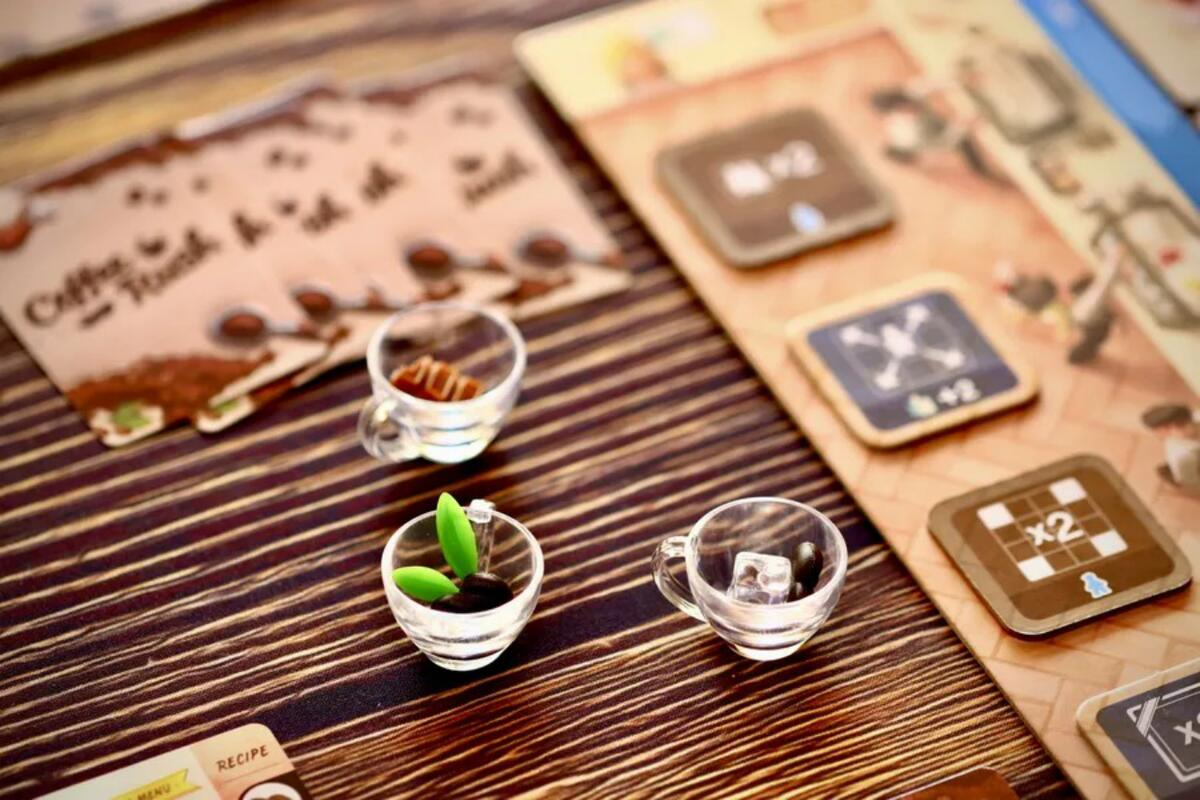
\includegraphics[width=5.2cm]{img/copertine/agd-coffee}};
  \node[polaroid, rotate=5]   at (\W/2+.2,\H-3.6) {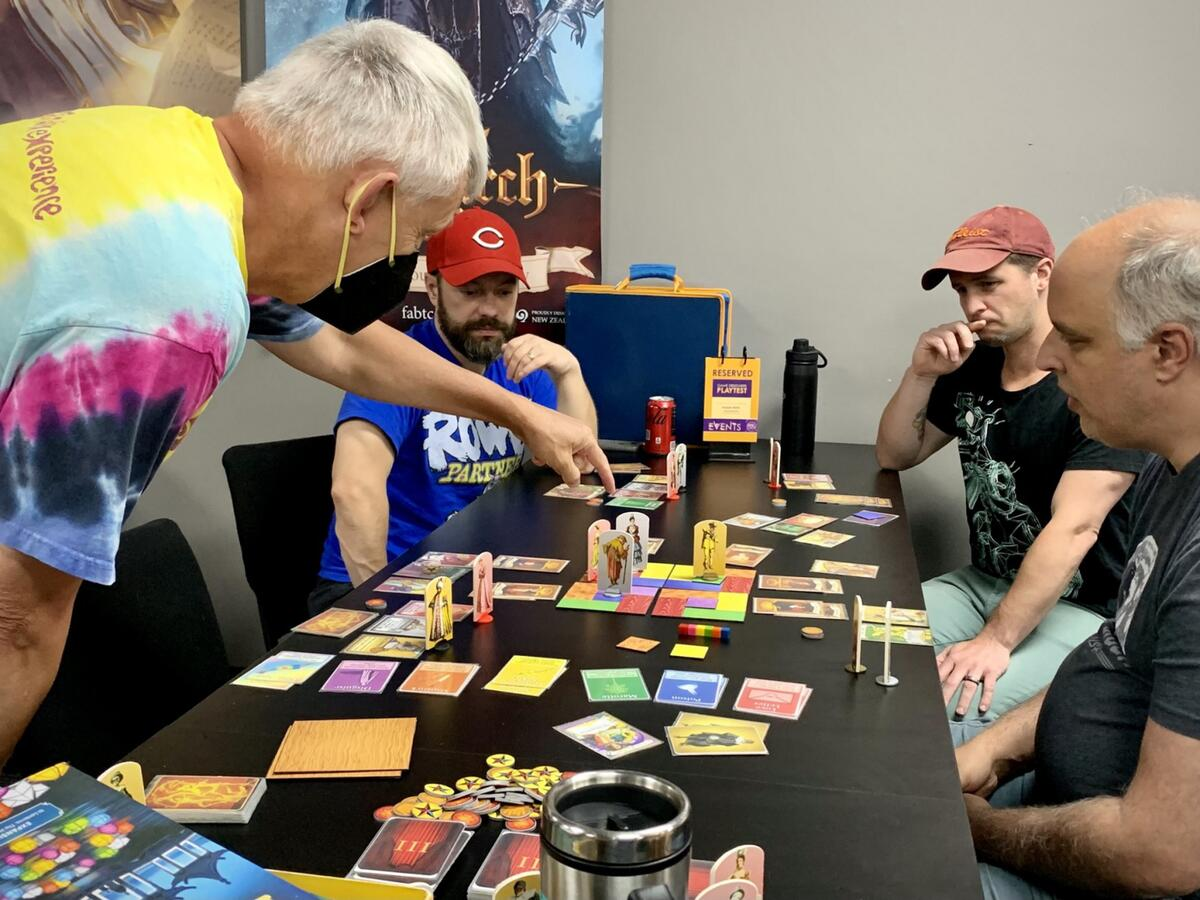
\includegraphics[width=4.6cm]{img/copertine/agd-playtest}};
  \node[polaroid, rotate=-3]  at (\W-4.2,\H-4.9) {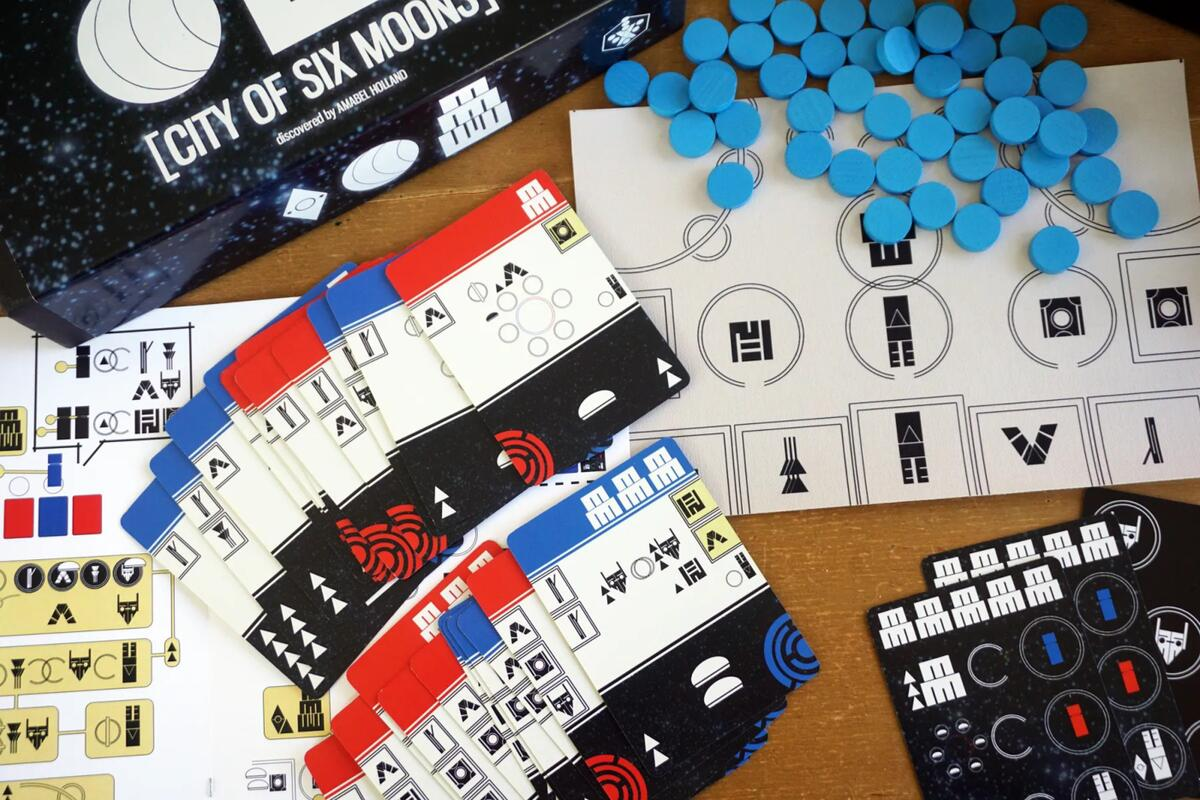
\includegraphics[width=5.0cm]{img/copertine/agd-city}};
  \node[polaroid, rotate=6]   at (3.8,7.9)  {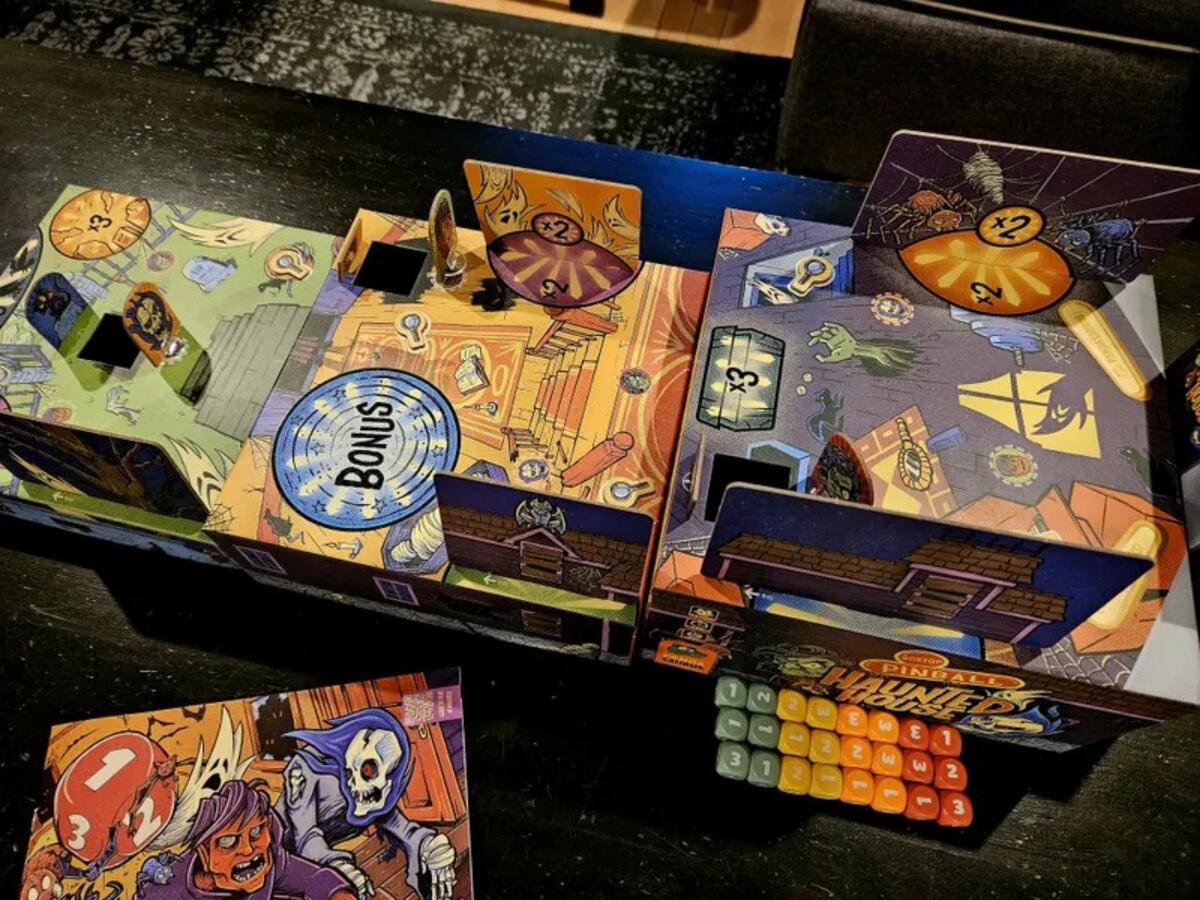
\includegraphics[width=4.8cm]{img/copertine/agd-pinball}};
  \node[polaroid, rotate=-4]  at (\W/2+.4,7.2) {
\includegraphics[width=4.6cm]{img/copertine/agd-larp}};
  \node[polaroid, rotate=4]   at (\W-4.0,7.8)  {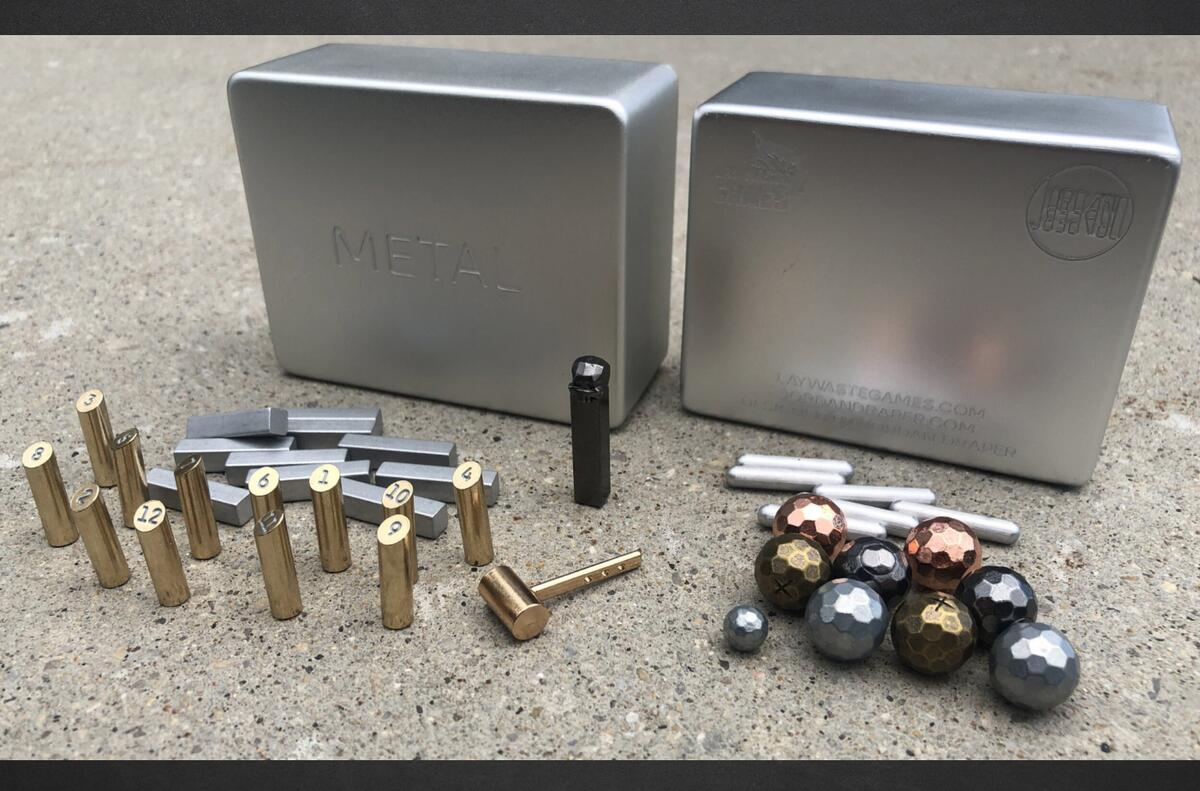
\includegraphics[width=4.8cm]{img/copertine/agd-metal}};
}

% Professioni: la rete dei mestieri
\def\copertina@professioni{%
  \fill[copTeal] (0,0) rectangle (\W,\H);
  \foreach \k in {1,...,9} \draw[copTealLight, opacity=.12, line width=.8pt] (\W/2,\H/2) circle (\k*1.6);
  \foreach \x/\y/\t/\i [count=\n] in {
      3.6/\H-3.6/Game designer/d, .5*\W/\H-2.6/Level designer/l, \W-3.6/\H-3.6/Narrative designer/n,
      3.6/4.4/Character animator/a, .5*\W/3.4/Programmatore/p, \W-3.6/4.4/3D artist/c} {
    \draw[copTealLight, line width=1.2pt, opacity=.6] (\x,\y) -- (.5*\W,.5*\H);
    \fill[white] (\x,\y) circle (1.35);
    \fill[copTealLight] (\x,\y) circle (1.15);
    \node[text=white, font=\sffamily\bfseries\small, below] at (\x,\y-1.45) {\t};
    \begin{scope}[shift={(\x,\y)}]
      \ifnum\n=1 \pic[fill=white, scale=.95, rotate=10] at (0,0) {dado5}; \fi
      \ifnum\n=2 \pic[scale=.55] at (0,-.6) {cubo}; \fi
      \ifnum\n=3 \node[fill=white, rounded corners=5pt, text=copTeal, font=\bfseries\Large, inner sep=4pt] at (0,0) {``\,\dots''}; \fi
      \ifnum\n=4 \begin{scope}[white, line width=2pt, line cap=round]
                 \fill (0,.55) circle (.2); \draw (0,.35) -- (0,-.2) -- (-.35,-.65); \draw (0,-.2) -- (.4,-.6);
                 \draw (-.45,.25) -- (0,.15) -- (.45,.4); \end{scope} \fi
      \ifnum\n=5 \node[text=white, font=\ttfamily\bfseries\LARGE] at (0,0) {\{\,\}}; \fi
      \ifnum\n=6 \begin{scope}[white, line width=1.4pt, scale=.55]
                 \draw (0,-1) -- (.87,-.5) -- (.87,.5) -- (0,0) -- cycle; \draw (0,-1) -- (-.87,-.5) -- (-.87,.5) -- (0,0);
                 \draw (-.87,.5) -- (0,1) -- (.87,.5); \end{scope} \fi
    \end{scope}
  }
}

% Game Design: flowchart, blockout e un rullino di immagini
\def\copertina@gamedesign{%
  \fill[copSlate] (0,0) rectangle (\W,\H);
  \draw[white, opacity=.05, step=1] (0,0) grid (\W,\H);
  % flowchart in alto
  \begin{scope}[shift={(0,\H-3.3)}, every node/.style={font=\sffamily\bfseries\small, text=copSlate}]
    \node[fill=copCyan, rounded corners=8pt, minimum width=2.2cm, minimum height=.9cm] (s) at (2.6,0) {Start};
    \node[fill=white, minimum width=2.6cm, minimum height=.9cm] (r) at (6.8,0) {Ricerca};
    \node[fill=copGold, diamond, aspect=1.7, inner sep=1.5pt] (d) at (11.2,0) {Funziona?};
    \node[fill=white, minimum width=2.4cm, minimum height=.9cm] (i) at (11.2,-2.2) {Itera};
    \node[fill=copCyan, rounded corners=8pt, minimum width=2.2cm, minimum height=.9cm] (e) at (15.8,0) {Vision};
    \draw[-{Stealth[length=3mm]}, white, line width=1.1pt] (s) -- (r);
    \draw[-{Stealth[length=3mm]}, white, line width=1.1pt] (r) -- (d);
    \draw[-{Stealth[length=3mm]}, white, line width=1.1pt] (d) -- node[above, text=white, font=\sffamily\scriptsize] {s\`i} (e);
    \draw[-{Stealth[length=3mm]}, white, line width=1.1pt] (d) -- node[right, text=white, font=\sffamily\scriptsize] {no} (i);
    \draw[-{Stealth[length=3mm]}, white, line width=1.1pt] (i) -| (r);
  \end{scope}
  % blockout isometrico ai lati
  \foreach \x/\y/\s in {1.6/.5*\H+5.6/.8, 2.6/.5*\H+5.1/.55, \W-1.8/.5*\H+5.4/.9, \W-2.9/.5*\H+5.0/.5}
    \pic[scale=\s] at (\x,\y) {cubo};
  % rullino
  \fill[black] (0,1.0) rectangle (\W,6.4);
  \foreach \k in {0,...,26} {
    \fill[copSlate!40] (.3+\k*.8,1.2) rectangle ++(.45,.3);
    \fill[copSlate!40] (.3+\k*.8,5.9) rectangle ++(.45,.3);
  }
  \foreach \f/\x in {gd-blockout/2.9, gd-uncharted/8.2, gd-interior/13.5, gd-liesofp/18.6}
    \node[inner sep=0pt] at (\x,3.7) {\includegraphics[height=3.9cm,width=4.9cm,keepaspectratio]{img/copertine/\f}};
}

% Revisioni: un foglio corretto a penna rossa
\def\copertina@revisioni{%
  \fill[copPaper] (0,0) rectangle (\W,\H);
  \foreach \k in {1,...,34} \draw[copRule, line width=.5pt] (0,\k*0.8) -- (\W,\k*0.8);
  \draw[copPen!70, line width=.8pt] (2.6,0) -- (2.6,\H);
  % righe di testo stilizzate in alto e in basso
  \foreach \y/\l in {\H-2.0/14, \H-2.8/16.5, \H-3.6/12, \H-4.4/15.5, \H-5.2/9,
                     6.4/15, 5.6/13, 4.8/16, 4.0/11, 3.2/14.5, 2.4/8} {
    \fill[black!45, rounded corners=1pt] (3.2,\y-.12) rectangle ++(\l,.24);
  }
  % correzioni
  \draw[copPen, line width=1.6pt, decorate, decoration={zigzag, amplitude=1.2pt, segment length=4pt}]
    (6,\H-2.8) -- (13.5,\H-2.8);
  \draw[copPen, line width=1.4pt] (10.6,\H-4.4) ellipse (2.8 and .45);
  \draw[copPen, line width=1.6pt, decorate, decoration={zigzag, amplitude=1.2pt, segment length=4pt}]
    (4.5,4.8) -- (12.5,4.8);
  \draw[copPen, line width=1.4pt] (8.8,2.4) ellipse (3 and .45);
  \node[text=copPen, font=\sffamily\bfseries\Huge, rotate=8] at (1.3,\H-3.6) {!};
  \node[text=copPen, font=\sffamily\bfseries\Huge, rotate=-6] at (1.3,4.0) {?};
  \foreach \x/\y in {19.4/\H-2.0, 19.4/6.4, 19.4/3.2}
    \draw[green!50!black, line width=2.4pt, line cap=round] (\x-.35,\y) -- (\x-.05,\y-.3) -- (\x+.5,\y+.45);
  % post-it
  \foreach \x/\y/\a/\t in {\W-3.4/\H-6.6/-6/Mostra{,} non scrivere!, 4.4/8.4/5/Fonte?, \W-4.0/8.0/4/Perch\'e?} {
    \node[fill=copPostit, drop shadow={opacity=.3}, rotate=\a, minimum width=3.6cm, minimum height=2.2cm,
          text width=3.2cm, align=center, font=\sffamily\bfseries\itshape\large, text=copPen] at (\x,\y) {\t};
  }
}

% --- Modi: volume autonomo o pagina di parte --------------------------------
\def\copertina@pannello{%
  \fill[white, opacity=.93, rounded corners=14pt, drop shadow={opacity=.35}]
    (2.2,\H/2-4.6) rectangle (\W-2.2,\H/2+4.6);}

\def\copertina@modo@libro#1{%
  \copertina@pannello
  \edef\copcol{\csname copertina@col@#1\endcsname}%
  \pgfmathsetmacro{\TW}{\W-6}%
  \fill[\copcol] (2.2,\H/2+3.4) rectangle (\W-2.2,\H/2+3.55);
  \node[text=\copcol, font=\sffamily\bfseries\large, anchor=south] at (\W/2,\H/2+3.7)
    {\csname copertina@vol@#1\endcsname};
  \node[text=\copcol, font=\sffamily\bfseries\fontsize{30}{34}\selectfont, text width=\TW cm,
        align=center] at (\W/2,\H/2+1.1) {\csname copertina@titolo@#1\endcsname};
  \node[text=black!70, font=\sffamily\large, text width=\TW cm, align=center]
    at (\W/2,\H/2-1.6) {\csname copertina@sotto@#1\endcsname};
  \fill[\copcol] (2.2,\H/2-3.0) rectangle (\W-2.2,\H/2-2.85);
  \node[text=black!80, font=\sffamily\bfseries\Large] at (\W/2,\H/2-3.75) {Lorenzo Vergata};
}

% Nella pagina di parte il testo stampato da \part cade poco sopra il centro
\def\copertina@modo@parte#1{%
  \fill[white, opacity=.93, rounded corners=14pt, drop shadow={opacity=.35}]
    (2.2,\H/2-0.4) rectangle (\W-2.2,\H/2+5.6);
  \edef\copcol{\csname copertina@col@#1\endcsname}%
  \fill[\copcol] (2.2,\H/2+0.4) rectangle (\W-2.2,\H/2+0.55);}

\newcommand{\disegnacopertina}[2]{%
  \begin{tikzpicture}[remember picture, overlay]
    \begin{scope}[shift={(current page.south west)}]
      \pgfmathsetmacro{\W}{\paperwidth/1cm}%
      \pgfmathsetmacro{\H}{\paperheight/1cm}%
      \csname copertina@#1\endcsname
      \csname copertina@modo@#2\endcsname{#1}%
    \end{scope}
  \end{tikzpicture}}

% Copertina a tutta pagina di un volume
\newcommand{\copertinaLibro}[1]{%
  \pagenumbering{Alph}%
  \begin{titlepage}
    \thispagestyle{empty}%
    \disegnacopertina{#1}{libro}%
    \null
  \end{titlepage}%
  \pagenumbering{arabic}}

% Pagina di parte illustrata (libro completo)
\newcommand{\partart}{}
\pretocmd{\@part}{\partart}{}{\PackageWarning{copertine}{Impossibile illustrare le parti}}
\pretocmd{\@spart}{\partart}{}{}
\newcommand{\parteillustrata}[2]{%
  \gdef\partart{\thispagestyle{empty}\disegnacopertina{#1}{parte}}%
  \part{#2}%
  \gdef\partart{}}
\makeatother



\title{Fondamenti di Unreal Engine}
\author{Lorenzo Vergata}
\date{\today}
\hypersetup{pdftitle={Fondamenti di Unreal Engine}, pdfauthor={Lorenzo Vergata}}

\begin{document}

    \copertinaLibro{unreal}
    \maketitle
    \tableofcontents

    % Contenuto della parte "Fondamenti di Unreal Engine".
% Incluso sia dal libro completo (main.tex) sia dal volume autonomo corrispondente.
\renewcommand{\thechapter}{1.\arabic{chapter}} \renewcommand{\theHchapter}{ue.\arabic{chapter}} \setcounter{chapter}{0}
% =====================================================================
%  Fondamenti di Unreal Engine, lezione 1 — Introduzione a Unreal
%  Engine: che cos'è un game engine, come si arriva a un'immagine sullo
%  schermo, chi usa l'engine in una produzione, da che cosa è formato un
%  gioco, e il primo contatto con l'editor.
%  Prima lezione del corso breve di introduzione a Unreal Engine (focus
%  sui Blueprints), online su Zoom, dalle 17 alle 19 circa, condotta da
%  Igor, ex studente di game design ed ex level designer di Steel Seed.
%  Contenuti, nell'ordine della lezione: presentazioni; software e game
%  engine; scripting e Blueprint; il rendering 3D (poligoni, vertex
%  shading, rasterizzazione, fragment shading, UV); il real time
%  rendering e i frame; Unreal Engine, i suoi giochi, la prototipazione
%  e il caso Expedition 33; gli engine proprietari di una volta; Unreal
%  nel cinema; il game loop; la produzione (pre-produzione, indie, AA,
%  AAA, outsourcing) e i ruoli che toccano l'engine; l'attività in
%  classe "da che cosa è formato un gioco" (attori, meccaniche, spazi,
%  obiettivi, regole, tempo; MDA); le domande prima della pausa (il
%  tempo come regola, il bilanciamento e il QA, The Midnight Walk e la
%  stop motion, il tempismo delle uscite); il download della 5.5; dopo
%  la pausa le risorse (documentazione, learning, Fab, materiale
%  didattico); un po' di teoria (Play in Editor, delta seconds); il
%  Project Browser e i template; l'interfaccia dell'editor; il
%  transform, gli assi, lo snapping, la navigazione, duplicare,
%  raggruppare, l'Outliner; l'esercitazione dei tre tavoli; il
%  salvataggio e la chiusura.
%  Fonte: trascrizione automatica della prima lezione (UE1), circa due
%  ore. Integrazioni dal libro "Blueprints Visual Scripting for Unreal
%  Engine 5" (Romero, Sewell), segnalate come approfondimenti.
%
%  Pacchetti richiesti nel preambolo del libro (già presenti nel
%  main.tex): \usepackage{booktabs}, \usepackage{tikz} con
%    \usetikzlibrary{shapes.geometric,shapes.symbols,shapes.misc,
%      arrows.meta,positioning,calc,fit}
%  (le librerie vanno caricate nel preambolo, non nel capitolo).
%  Consigliati, come per gli altri capitoli: \usepackage[italian]{babel}
%  e \usepackage[T1]{fontenc} (il capitolo compila anche senza).
%
%  Collocazione nel libro: parte "Fondamenti di Unreal Engine", primo
%  capitolo (numerazione propria 1.1). Nel file principale del libro,
%  subito dopo il \part e il \setcounter della parte:
%
%    % =====================================================================
%  Fondamenti di Unreal Engine, lezione 1 — Introduzione a Unreal
%  Engine: che cos'è un game engine, come si arriva a un'immagine sullo
%  schermo, chi usa l'engine in una produzione, da che cosa è formato un
%  gioco, e il primo contatto con l'editor.
%  Prima lezione del corso breve di introduzione a Unreal Engine (focus
%  sui Blueprints), online su Zoom, dalle 17 alle 19 circa, condotta da
%  Igor, ex studente di game design ed ex level designer di Steel Seed.
%  Contenuti, nell'ordine della lezione: presentazioni; software e game
%  engine; scripting e Blueprint; il rendering 3D (poligoni, vertex
%  shading, rasterizzazione, fragment shading, UV); il real time
%  rendering e i frame; Unreal Engine, i suoi giochi, la prototipazione
%  e il caso Expedition 33; gli engine proprietari di una volta; Unreal
%  nel cinema; il game loop; la produzione (pre-produzione, indie, AA,
%  AAA, outsourcing) e i ruoli che toccano l'engine; l'attività in
%  classe "da che cosa è formato un gioco" (attori, meccaniche, spazi,
%  obiettivi, regole, tempo; MDA); le domande prima della pausa (il
%  tempo come regola, il bilanciamento e il QA, The Midnight Walk e la
%  stop motion, il tempismo delle uscite); il download della 5.5; dopo
%  la pausa le risorse (documentazione, learning, Fab, materiale
%  didattico); un po' di teoria (Play in Editor, delta seconds); il
%  Project Browser e i template; l'interfaccia dell'editor; il
%  transform, gli assi, lo snapping, la navigazione, duplicare,
%  raggruppare, l'Outliner; l'esercitazione dei tre tavoli; il
%  salvataggio e la chiusura.
%  Fonte: trascrizione automatica della prima lezione (UE1), circa due
%  ore. Integrazioni dal libro "Blueprints Visual Scripting for Unreal
%  Engine 5" (Romero, Sewell), segnalate come approfondimenti.
%
%  Pacchetti richiesti nel preambolo del libro (già presenti nel
%  main.tex): \usepackage{booktabs}, \usepackage{tikz} con
%    \usetikzlibrary{shapes.geometric,shapes.symbols,shapes.misc,
%      arrows.meta,positioning,calc,fit}
%  (le librerie vanno caricate nel preambolo, non nel capitolo).
%  Consigliati, come per gli altri capitoli: \usepackage[italian]{babel}
%  e \usepackage[T1]{fontenc} (il capitolo compila anche senza).
%
%  Collocazione nel libro: parte "Fondamenti di Unreal Engine", primo
%  capitolo (numerazione propria 1.1). Nel file principale del libro,
%  subito dopo il \part e il \setcounter della parte:
%
%    \input{UE/UE1_introduzione_a_unreal_engine}
%
%  Tutte le etichette di questo capitolo hanno il prefisso "ue1:"
%  (ue1:cap:..., ue1:sec:..., ue1:fig:..., ue1:tab:...), e tutti gli
%  stili TikZ hanno il prefisso "ue1" (ue1box, ue1arr, ...) per non
%  collidere con chiavi native di TikZ. Il capitolo è autonomo: non
%  contiene \ref verso altri capitoli.
%  Le figure sono ricostruzioni schematiche di quanto mostrato e detto a
%  lezione, non copie delle slide del docente. Dove la trascrizione è
%  troppo rovinata per ricostruire un dettaglio, il capitolo lo dice
%  invece di inventarlo.
% =====================================================================

\chapter[Introduzione a Unreal Engine]{Introduzione a Unreal Engine: che cos'è un
engine, chi lo usa, e il primo contatto con l'editor}
\label{ue1:cap:intro}

Questa è la \textbf{prima lezione} del corso breve di \textbf{introduzione a Unreal
Engine}, un corso che ha il suo centro nei \textbf{Blueprint}, il sistema di
programmazione visuale ``a nodi'' dell'engine di Epic Games. La lezione ha due metà
molto diverse. La prima è teorica e larga: che cos'è un \emph{software}, che cos'è un
\emph{game engine}, come un modello fatto di poligoni diventa un'immagine sullo
schermo, perché Unreal è oggi l'engine più diffuso, quali figure di una produzione lo
usano e per che cosa, e infine, con un'attività in classe, da che cosa è formato un
gioco. La seconda metà è pratica: si scarica Unreal Engine 5.5, si guardano le risorse
che Epic mette a disposizione (la documentazione, i corsi gratuiti, il negozio di
\emph{asset} Fab), si crea un primo progetto vuoto e si impara a muoversi nell'editor:
piazzare un cubo, spostarlo, ruotarlo, scalarlo, duplicarlo, raggrupparlo, ordinarlo
in cartelle. La lezione si chiude con un'esercitazione: arredare un piccolo
ristorante con tre tavoli e le loro sedie.

Il docente è \textbf{Igor}\footnote{Il docente si presenta come ``Igor Ripanti''; il
cognome è quello della trascrizione automatica, che altrove storpia quasi tutti i nomi
propri, e il capitolo non è in grado di verificarlo.}, che si presenta come ex alunno
della stessa scuola degli studenti, ``precisamente per quanto riguarda game
design''\footnote{La trascrizione dice ``sono stato un alunno di Live'': il nome della
scuola è con ogni probabilità storpiato.}. Ha lavorato a \textbf{\emph{Steel Seed}},
``principalmente come \emph{level designer}''; ma ``essendo un ambiente indie'' faceva
``un po' di tutto'', anche programmazione e \emph{scripting}, e quindi ha fatto ``uso
intensivo'' di Unreal Engine ``e di tutte le sue feature''. Il corso è diviso tra due
docenti: con Igor la parte di programmazione e di ``piccole feature''; con
\textbf{Davide}, a partire dal 26 del mese, una parte ``un po' più artistica''. Le
lezioni si alternano: il giovedì successivo gli studenti saranno di nuovo con Igor, il
martedì dopo con Davide.

La lezione è \textbf{online}, su Zoom, con un server Discord del corso per i
materiali e le domande; inizia poco dopo le 17 e finisce alle 19, con una pausa di una
decina di minuti verso le 17 e mezza\footnote{Igor, credendo per errore che la lezione
finisse alle 18 (``sono da un altro corso che finiva alle 18''), dopo la pausa annuncia
che ``manca mezz'ora alla fine''; gli studenti lo correggono (``nella mail c'era
scritto'' alle 19), e il docente ha ``un'altra ora'' per la parte pratica.}. Gli
studenti sono tutti \textbf{nuovi iscritti al primo anno}, di corsi diversi: game
design (la maggioranza), narrative design, character animation, 3D art e
programmazione. Il corso breve, in altre parole, è comune a figure che in una
produzione useranno Unreal in modi molto diversi, ed è proprio da questa varietà che
Igor parte.

Tre avvertenze di lettura. La prima: la trascrizione è automatica e storpia moltissimi
nomi. Unreal diventa ``Arreal'', ``Arial Engine'', ``ArrayLange'', ``ArrayLab'',
``Arrival Engine'', ``Arrial'', ``Ariane Engine'', ``Riala'' e ``a Real Engine'';
\emph{Clair Obscur: Expedition 33} è ``Expedition'' e ``Spedisce 33''; Sandfall
Interactive è ``Send Follow Interactive''; \emph{shader} è anche ``scender''. Dove la
ricostruzione è sicura il capitolo usa la forma corretta e, la prima volta, lo segnala
in nota; dove non lo è riporta la forma della trascrizione e lo dice. La seconda: in
più punti la registrazione contiene lunghi blocchi di testo senza senso e ripetuto
(``qual è la risposta che ci può essere?'', ``a parte il plus time\ldots''): sono
artefatti del riconoscimento vocale durante la pausa e i momenti di lavoro
individuale, e il capitolo li ignora. La terza: la seconda metà della lezione è una
dimostrazione dal vivo nell'editor; il capitolo ricostruisce i passaggi da ciò che Igor
dice mentre li fa, e li completa, dove serve, con i nomi esatti dei comandi.

\paragraph{Come leggere questo capitolo.} Il capitolo segue l'ordine della lezione.
Le figure ricostruiscono gli schemi spiegati a voce o sulle slide (la pipeline di
rendering, il \emph{game loop}, gli elementi di un gioco, l'interfaccia dell'editor,
il \emph{transform}); le tabelle riassumono i ruoli della produzione e le scorciatoie
da tastiera della seconda parte. Qua e là, dei paragrafi di \textbf{approfondimento}
collegano la lezione al libro \emph{Blueprints Visual Scripting for Unreal Engine 5}
di Marcos Romero e Brenden Sewell, che sarà il testo di riferimento per questa parte
del libro, e a qualche nozione tecnica generale; sono segnalati come tali e non fanno
parte della lezione.

Il percorso del capitolo:
\begin{enumerate}
  \item le presentazioni e le esperienze degli studenti (sezione
        \ref{ue1:sec:presentazioni});
  \item il \textbf{software}, il \textbf{game engine} e lo \textbf{scripting}, con i
        Blueprint (sezione \ref{ue1:sec:engine});
  \item il \textbf{rendering 3D}: poligoni, \emph{vertex shading}, rasterizzazione,
        \emph{fragment shading}; poi il \emph{real time rendering} e i \emph{frame}
        (sezioni \ref{ue1:sec:rendering} e~\ref{ue1:sec:realtime});
  \item \textbf{Unreal Engine}: perché è così usato, la prototipazione, i giochi, gli
        engine di una volta, il cinema, il \textbf{game loop} (sezioni
        da~\ref{ue1:sec:unreal} a~\ref{ue1:sec:gameloop});
  \item la \textbf{produzione} e i \textbf{ruoli} che toccano l'engine (sezioni
        \ref{ue1:sec:produzione} e~\ref{ue1:sec:ruoli});
  \item l'attività in classe: \textbf{da che cosa è formato un gioco}, e le domande
        prima della pausa (sezioni \ref{ue1:sec:elementi} e~\ref{ue1:sec:domande});
  \item il \textbf{download} della 5.5, le \textbf{risorse} (documentazione,
        \emph{learning}, Fab) e un po' di teoria sul \emph{Play in Editor} e sul
        \emph{delta time} (sezioni da~\ref{ue1:sec:download} a~\ref{ue1:sec:pie});
  \item il primo contatto con l'\textbf{editor}: il progetto, l'interfaccia, il
        \textbf{transform}, la navigazione, l'organizzazione (sezioni
        da~\ref{ue1:sec:progetto} a~\ref{ue1:sec:outliner});
  \item l'\textbf{esercitazione dei tre tavoli}, il salvataggio e la chiusura (sezioni
        \ref{ue1:sec:esercitazione} e~\ref{ue1:sec:chiusura}).
\end{enumerate}

% ---------------------------------------------------------------------
\section{Presentazioni: chi c'è, e chi ha già aperto un engine}
\label{ue1:sec:presentazioni}

La lezione comincia con qualche minuto di attesa (``aspettiamo cinque, dieci minuti''),
un appello e una richiesta: accendere la webcam, ``così almeno ci vediamo un po' in
faccia''. A chi non ha una webcam Igor suggerisce le applicazioni che trasformano il
telefono in una webcam, ``come se ti facessi una videochiamata'': lui usa di solito
\emph{Iriun}\footnote{Nella trascrizione ``Ingur'' e ``Iruin''; si tratta con ogni
probabilità di \emph{Iriun Webcam}, un'applicazione gratuita che fa esattamente
questo.}. I lavori in corso nell'edificio del docente producono ``rumori molesti'' per
tutta la lezione, e Igor se ne scusa.

Poi il giro di presentazioni: nome, corso, ``un piccolo background''. Tutti sono iscritti
al primo anno; i corsi sono game design, character animation, narrative design (più di
uno), 3D art e programmazione. ``C'è una bella quantità di nuovi compagni di design'',
commenta Igor, ``quindi avremo pane per i nostri denti'', oltre ovviamente a 3D art e
programmazione.

\paragraph{Chi ha già usato un engine?} La domanda successiva è se qualcuno abbia ``mai
aperto un software di \emph{develop} per i videogiochi'': Unity, Godot, ``in
generale''. Qualcuno ha provato Godot; qualcuno un po' di Unity, seguendo un corso
online ``molto veloce'' e facendo ``un paio di giochini'', un \emph{platform} e un clone
di \emph{Flappy Bird}, ``di 3D niente''; qualcuno è ``digiuno'', e qualcun altro ha
lavorato ``con roba presa da Fab''. Igor accoglie tutte le risposte allo stesso modo:
``ci sta assolutamente''. Fab, aggiunge, sarà uno dei temi di oggi, perché è ``una
risorsa incredibile'', soprattutto per le cose gratis, quelle in sconto e i contenuti
gratuiti del mese.

\paragraph{La mentalità prima degli strumenti.} A chi parte da zero Igor dà subito una
rassicurazione che vale per tutto il corso: ``l'importante è avere la mentalità''. In
programmazione, ``molto spesso'' si tratta ``semplicemente'' di imparare a usare gli
strumenti, mentre ``la logica fa da padrone''. Passare da un engine all'altro, o da
nessun engine al primo, è soprattutto ``riabituarsi a un nuovo campo di gioco''.

% ---------------------------------------------------------------------
\section{Software, game engine e scripting}
\label{ue1:sec:engine}

\paragraph{Che cos'è un software.} Igor parte dalla definizione più semplice possibile:
il \textbf{software} è ``quello che non è hardware, fondamentalmente''. È un insieme di
istruzioni, di dati e di programmi con funzionalità precise, che ci permettono di
creare cose: strumenti di 3D art come \textbf{Blender} e \textbf{Maya}, oppure
\emph{engine} come \textbf{Unreal Engine} e \textbf{Unity}.

\paragraph{L'engine come calderone.} Il \textbf{game engine} è ``il calderone, chiamiamolo
un po' così'', che riunisce tutte le facoltà di chi sviluppa (3D art, programmazione,
design) e le mette ``in un ambiente comune'', l'ambiente di sviluppo dell'engine. Gli
engine più noti sono \textbf{Unreal}, \textbf{Unity}, \textbf{Godot} e
\textbf{GameMaker}, e ognuno contiene al suo interno molte funzionalità: i
\textbf{motori fisici}, che gestiscono le \textbf{collisioni}; la gestione dei
\textbf{suoni}; le \textbf{animazioni}; il \textbf{networking}; l'\textbf{intelligenza
artificiale} dei personaggi. Nessuna di queste cose ``si fa da sola'': ci mettono le
mani gli sviluppatori, ``tramite lo \emph{scripting}''.

\paragraph{Lo scripting, e i Blueprint.} Lo \textbf{scripting} è ``la forma di
programmazione che ci permette di entrare in interazione e creare cose all'interno
dell'engine''. Esistono molti linguaggi: Igor cita il \textbf{C}, il \textbf{C\#}
(quello di Unity) e i \textbf{Blueprint}, che sono il tipo di \emph{scripting} di Unreal
Engine e l'oggetto di questo corso. Più avanti nella lezione (sezione~\ref{ue1:sec:ruoli})
Igor tornerà sul punto: in Unreal si può programmare anche in codice (in C++), ``ma noi
non lo useremo'', perché i Blueprint bastano ``tranquillamente'', sono usati anche dai
programmatori, e ``tanti giochi nel comparto indie'' sono fatti ``solo con Blueprint,
senza mai toccare una riga di codice''. I Blueprint sono un \textbf{linguaggio a nodi}:
``prendiamo proprio e colleghiamo tutti i nodini'' per dare un senso alla
programmazione.

\paragraph{Approfondimento: le due accezioni di ``Blueprint''.} Romero e Sewell, nel
primo capitolo di \emph{Blueprints Visual Scripting for Unreal Engine 5}, fanno notare
che in Unreal la parola \emph{Blueprint} ha due significati. È il nome del
\textbf{linguaggio di scripting visuale} creato da Epic Games; ed è anche il nome di un
\textbf{tipo di oggetto di gioco} creato con quel linguaggio. I Blueprint di questo
secondo tipo sono di due specie: il \textbf{Level Blueprint}, uno per ogni livello del
gioco (non se ne possono creare altri separati), e le \textbf{Blueprint Class}, che
servono a creare oggetti interattivi riutilizzabili in qualunque livello. Un progetto di
Unreal Engine 5, aggiungono gli autori, si può sviluppare in Blueprint, in C++ o in una
combinazione dei due: si può aggiungere codice C++ a un progetto Blueprint e viceversa.
La scelta di partire dai Blueprint, quindi, non chiude nessuna porta.

% ---------------------------------------------------------------------
\section{Il rendering 3D: dai poligoni ai pixel}
\label{ue1:sec:rendering}

Un'applicazione grafica come un gioco 3D ha una particolarità: il \textbf{3D
rendering}, cioè ``la fase finale dello sviluppo di un'immagine''. È il processo che
prende un \textbf{\emph{3D asset}} (``per il linguaggio un po' più tecnico'') e ci
presenta davanti la scena vera e propria, con gli oggetti creati dai 3D artist ``che
hanno faticato tanto per poterlo fare''. Quegli oggetti sono formati da
\textbf{poligoni}.

\paragraph{Quanti poligoni ha questo oggetto?} Igor chiede se qualcuno ha mai sentito
parlare del numero di poligoni di un modello. Uno studente sì: gli sono capitati ``dei
video di ottimizzazione'' su come diminuire i poligoni ``per cercare di diminuire il
\emph{lag}''. ``Esatto, bravissimo.'' La regola è semplice, e Igor la dice con una
battuta: ``se mai doveste avere il caso fortuito di avere un cubo con due milioni di
poligoni, sappiate che il vostro gioco esploderà, probabilmente''. Nella
\textbf{viewport} (``un elemento che poi vedremo'': la finestra in cui l'engine, ma
anche Blender mentre si modella, mostra la scena) vale sempre lo stesso compromesso:
\textbf{più poligoni ci sono, più l'immagine è precisa, ma più è pesante da
renderizzare}.

\paragraph{Le tre fasi.} Il rendering di un'immagine passa per molti passaggi; ``noi oggi''
ne guardiamo tre principali (figura~\ref{ue1:fig:pipeline}).
\begin{enumerate}
  \item \textbf{\emph{Vertex shading}.} Le immagini e i modelli sono formati
        principalmente da \textbf{triangoli}, e i triangoli sono formati da
        \textbf{vertici}. I vertici definiscono la forma: in questa fase si
        identificano e si posizionano i tre punti di ogni triangolo.
  \item \textbf{Rasterizzazione.} Il triangolo così definito viene
        \emph{rasterizzato}: si stabilisce quali \textbf{pixel} dello schermo cadono
        dentro quel triangolino. Igor la spiega a partire dalla grafica 2D (``qualcuno
        ha fatto grafica?'', e una studentessa laureata in grafica conferma). Un'immagine
        \textbf{raster}, come quelle di Photoshop, è fatta di pixel; un'immagine
        \textbf{vettoriale} è fatta di vettori. La differenza: se si ingrandisce
        (``strecciate'') un'immagine raster, diventa ``sgranatissima''; un'immagine
        vettoriale la si può ingrandire ``quanto volete'' e resta uguale. Gli schermi,
        però, sono fatti di pixel: per questo i triangoli vanno rasterizzati.
  \item \textbf{\emph{Fragment shading}.} È la fase finale, quella ``vicina alla
        visualizzazione''. Ai \textbf{frammenti} (``poligoni, triangoli, chiamateli
        come vi pare'') si applicano i \textbf{colori}, la \textbf{luce}, le
        \textbf{ombreggiature} e i \textbf{riflessi}, tenendo conto della posizione
        della camera. È anche ``una parte molto artistica'', perché Unreal lavora molto
        sulla resa della luce: si possono piazzare luci, gestire come la luce entra in
        una stanza, e così via.
\end{enumerate}

\begin{figure}[htbp]
\centering
\begin{tikzpicture}[
  font=\small,
  ue1box/.style={draw, thick, rounded corners=3pt, minimum height=1.5cm,
               text width=2.6cm, align=center},
  ue1io/.style={draw, thick, dashed, rounded corners=3pt, fill=gray!10,
               minimum height=1.5cm, text width=2.0cm, align=center},
  ue1arr/.style={-{Stealth[length=3mm]}, thick}
]
  \node[ue1io] (m) {\textbf{Modello 3D}\\poligoni\\(triangoli)};
  \node[ue1box, right=0.5cm of m] (v) {\textbf{1. Vertex shading}\\i vertici
    definiscono la forma dei triangoli};
  \node[ue1box, right=0.5cm of v] (r) {\textbf{2. Rasterizzazione}\\quali pixel
    cadono dentro ogni triangolo};
  \node[ue1box, right=0.5cm of r] (f) {\textbf{3. Fragment shading}\\colore, luce,
    ombre, riflessi};
  \node[ue1io, below=0.8cm of f] (s) {\textbf{Immagine}\\sullo schermo\\(pixel)};
  \draw[ue1arr] (m) -- (v);
  \draw[ue1arr] (v) -- (r);
  \draw[ue1arr] (r) -- (f);
  \draw[ue1arr] (f) -- (s);
  \node[below=0.9cm of v, text width=6.2cm, align=left, font=\footnotesize] {Più
    poligoni $\Rightarrow$ immagine più precisa, ma più pesante da renderizzare
    (``un cubo con due milioni di poligoni'' fa esplodere il gioco).};
\end{tikzpicture}
\caption{Le tre fasi principali del rendering di cui parla Igor. Il processo reale ha
molti passaggi intermedi; la lezione si ferma a questi tre.}
\label{ue1:fig:pipeline}
\end{figure}

\paragraph{Per vertici o per frammenti.} Sulla slide, in basso a destra, ci sono due
versioni della stessa sfera illuminata. Nella prima la luce è calcolata \textbf{per
vertici}: la luce ``quasi'' lascia vedere i triangoli. Nella seconda è calcolata
\textbf{per frammenti}, cioè dopo il \emph{fragment shading}: la luce è ``molto più
diramata'', morbida, ``e fa sì che funzioni per bene''.

\paragraph{Le UV.} Igor accenna anche alle \textbf{UV}, di cui si parlerà più avanti nel
corso: sono ``delle mappe che i 3D artist creano'' e che permettono di dire come il
materiale si comporta sulla superficie del modello, come gestire e rifrangere la luce,
``questo materiale così'', e così via.

\paragraph{Approfondimento: che cosa sono le UV.} Per completezza (la lezione ci torna
solo di sfuggita): le \textbf{coordinate UV} sono il modo in cui la superficie di un
modello 3D viene ``srotolata'' su un piano a due dimensioni, come si apre la scatola di
cartone di un cubo. Le lettere U e V indicano i due assi di quel piano, per non
confonderli con gli X, Y e Z dello spazio 3D. Su quel piano si dipingono le
\emph{texture} (il colore, la rugosità, i dettagli in rilievo), che poi l'engine
``riavvolge'' sul modello durante il rendering. Un buon \emph{UV mapping} è il motivo
per cui una texture appare senza deformazioni o cuciture visibili.

% ---------------------------------------------------------------------
\section{Il \emph{real time rendering} e i \emph{frame}}
\label{ue1:sec:realtime}

In Unreal Engine il rendering è \textbf{in tempo reale}. Igor lo collega a un'esperienza
che molti studenti faranno: lo \emph{showreel}, soprattutto per chi diventerà 3D artist,
sarà ``molto accompagnato'' dal rendering di Unreal, con camere ed effetti ``fatti per
bene, scriptati'', che permettono di vedere gli oggetti ``alla massima qualità
possibile''. E come sempre: più alta è la qualità, più tempo ci vuole per renderizzare.
Il \emph{real time rendering} è il rendering che produce le immagini a una velocità
compresa, più o meno, tra i \textbf{20 e i 120 fotogrammi al secondo}.

\paragraph{Che cos'è un frame.} Un \textbf{frame} (fotogramma) è una singola immagine; la
\textbf{visualizzazione per frame} è un susseguirsi di immagini correlate l'una
all'altra che danno l'\textbf{illusione del movimento} sullo schermo. È lo stesso
principio dell'animazione: il cinema lavora a \textbf{24 \emph{frame} al secondo}
(``quando andate a vedere un film''), il gaming di solito a \textbf{30 o 60
\emph{fps}}, e c'è chi gioca a 120--144 \emph{fps} (``incredibili'', commenta Igor,
``l'\emph{fps} che se la tira tanto'').

\paragraph{Approfondimento: il budget di un frame.} Un modo utile per leggere questi
numeri è rovesciarli. A 30 \emph{fps} l'engine ha circa $1000/30 \approx 33$
millisecondi per produrre ogni immagine; a 60 \emph{fps} ne ha circa 16,7; a 120 circa
8,3. In quel tempo deve leggere gli input, aggiornare la logica di gioco (il
\emph{game loop} della sezione~\ref{ue1:sec:gameloop}) e renderizzare la scena. È per
questo che l'ottimizzazione (meno poligoni, meno luci dinamiche, nebbia più leggera)
non è un dettaglio tecnico ma una condizione per avere un gioco giocabile: tutto ciò che
non entra nel \emph{budget} fa scendere il \emph{frame rate}.

% ---------------------------------------------------------------------
\section{Unreal Engine: perché è così usato}
\label{ue1:sec:unreal}

Unreal Engine è ``il nostro bellissimo'' game engine, quello che si userà per tutto il
corso. È sviluppato da \textbf{Epic Games}, e per usarlo bisogna scaricare
l'\textbf{Epic Games Launcher} dal sito di Epic (lo si farà durante la lezione, sezione
\ref{ue1:sec:download}).

\paragraph{Il più usato.} È, dice Igor, ``proprio il più usato al momento'': ``gran parte
dei giochi moderni'', AA e AAA, tendono a usarlo. Una delle ragioni è che, essendo un
motore comune, Epic lo aggiorna continuamente, con nuove funzionalità come il
\textbf{Control Rig}, che permette per esempio di fare le animazioni in modo
procedurale. Nel launcher si vede: ogni volta propone una versione diversa da scaricare
(5.5, 5.6, 5.7\ldots), e il canale YouTube ufficiale di Unreal Engine pubblica a ogni
versione un video riassuntivo delle novità.

\paragraph{Un linguaggio comune.} La seconda ragione è che Unreal è un \textbf{linguaggio
comune}: permette ai professionisti di parlarsi e di produrre insieme. I designer, per
esempio, lo usano ``molto spesso per prototipare''. La \textbf{prototipazione} è una
fase ``molto importante'' della creazione di un gioco: ``tiro fuori l'idea dal
cappello'' e la si mette ``direttamente in engine'', usando lo \emph{scripting} per
vedere se ``questa idea che ho in testa funziona''. È ``il modo più veloce e più giusto
per capire subito se qualcosa funziona''. Poi ci sono molte altre figure che usano
l'engine nelle sue diverse caratteristiche (sezione~\ref{ue1:sec:ruoli}).

\paragraph{Alcuni giochi fatti in Unreal.} Sulla slide: \emph{A Way Out}, \emph{Ark},
\emph{Crash Bandicoot 4} (``per chi ha giocato, bellissimo'') e \emph{Fortnite}. Per
\emph{Fortnite} esiste anche una versione dell'engine, \textbf{Unreal Editor for
Fortnite} (UEFN), che permette di prendere le funzionalità del gioco e ``metterle
insieme''. Igor lo paragona a \textbf{Roblox}, che sta facendo ``un simile effetto'':
creare un \textbf{mega \emph{game template}}. Un \emph{game template} è ``il
\emph{pattern} di regole'', tutto ciò che forma il gioco, messo a disposizione delle
persone perché ci facciano ``quello che vogliono''.

\paragraph{Il caso \emph{Expedition 33}.} Igor chiede quale gioco fatto in Unreal sia
rimasto in testa agli studenti, e la risposta arriva subito: \textbf{\emph{Clair
Obscur: Expedition 33}}\footnote{Nella trascrizione quasi sempre solo ``Expedition'' o
``Expedition 33'', una volta ``Spedisce 33''.}. ``Benissimo, vedo che ci intendiamo.''
Il gioco, racconta Igor, è nato da persone che, ``per quanto dicano loro'', hanno
detto: ``non sapevamo fare un gioco, e ci siamo messi a guardare YouTube''. Igor mostra
il video del \textbf{prototipo} di \emph{Expedition 33} fatto in Unreal Engine (dopo la
solita pubblicità): è lo stadio che si affronta ``molto spesso all'inizio di una
produzione'', quello in cui ``non ci interessa se è bello o brutto, è importante che
funzioni''. Unreal permette proprio questo: mettere subito in campo le cose più usate
del gaming.

\paragraph{Le cose comuni.} Ci sono infatti tante cose ``comuni all'interno del nostro
panorama videoludico''. Il \textbf{salto}, per esempio: ``quante volte in un gioco si
salta?''. C'è chi non lo usa, ma i giochi con il salto sono ``a bizzeffe''. Unreal,
creando una sorta di \emph{template} comune, facilita molto i primi passi.

% ---------------------------------------------------------------------
\section{Gli engine di una volta, e Unreal fuori dai videogiochi}
\label{ue1:sec:storia}

\paragraph{Quando ogni gioco aveva il suo engine.} ``Non siamo lì, ragazzi, nel 2004.'' Nei
vecchi giochi, ricorda Igor, si creavano engine \textbf{apposta}: un programmatore
doveva passare dalle linee di codice alla visualizzazione in 3D, ``in tutto un processo
che andava dai due ai tre anni''. E quegli engine erano poco riutilizzabili, perché
contenevano ``\emph{pattern} di regole molto fissati''. Si trovavano comunque modi
interessanti di riusarli: Igor cita, come ``piccola curiosità'', un gioco di Shrek per
PlayStation~2 (``Shrek~2'', si corregge) realizzato modificando il motore di un gioco
del \emph{Signore degli Anelli}\footnote{L'aneddoto è riportato come lo racconta Igor,
che lo introduce con ``io mi ricordo''; il capitolo non ha verificato quale gioco del
\emph{Signore degli Anelli} e quale versione di \emph{Shrek} siano coinvolti.}.

\paragraph{Gli engine proprietari.} Esistono poi gli engine \textbf{proprietari}, come
\textbf{Source} e \textbf{Source~2} di Valve (\emph{Half-Life}): sono ``loro'', di Valve,
ma la casa mette a disposizione gratuitamente gli strumenti per creare mappe, con
l'editor \textbf{Hammer}. Unreal, invece, mette a disposizione ``tante cose diverse''
per ``mettere subito la carne sul fuoco'' e facilitare il progetto.

\paragraph{Unreal nel cinema.} Oltre ai videogiochi, Unreal è ``molto usato'' nel
\textbf{\emph{filmmaking}} e nel \emph{videomaking}. Igor mostra uno spot di
motociclette (``della Indian''): le rocce intorno al motociclista ``non esistono'', sono
renderizzate in Unreal. È ``la classica storia del \emph{green screen}'', con dietro il
lavoro di chi è esperto di Unreal. Uno studente ricorda che anche \emph{The Batman} fu
girato in parte in questo modo, e Igor conferma che ``se ne parlò'': oggi è ``molto in
voga'', perché ``nessuno ha voglia di andare di nuovo in Islanda'' per avere delle
rocce molto belle; ci si fa le rocce pre-renderizzate.

\paragraph{Ottimizzazione contro dettaglio.} I processi, però, sono ``molto
differenziati''. Nei videogiochi si parla molto di \textbf{ottimizzazione}: modelli
\textbf{\emph{low poly}}, non pesantissimi e non precisissimi, ``belli da vedere ma
ottimizzati''. Nel \emph{filmmaking} l'ottimizzazione esiste, ma conta il
\textbf{dettaglio}, perché il risultato è ``solo una raffigurazione''. Un videogioco,
invece, è \textbf{un programma in esecuzione}: continui \emph{frame}, continue
interazioni, un continuo \emph{game loop}.

\paragraph{Le rocce che si vedono ovunque.} Una battuta tra sviluppatori: esistono rocce
che ``sono le stesse, perché sono bellissime''. Sono fatte in 4K e
\textbf{scannerizzate}: qualcuno si è messo letteralmente a fotografare le rocce, le ha
digitalizzate e le ha messe gratis sull'\emph{asset store}. ``E le vedete ovunque'':
``ormai sono riconoscibili'', fatte molto bene ma molto comuni.

\paragraph{Approfondimento: \emph{virtual production} e \emph{scan}.} Le due cose di cui
parla Igor hanno un nome. La prima è la \textbf{\emph{virtual production}}: invece di
aggiungere lo sfondo in post-produzione su un \emph{green screen}, si proietta in
tempo reale l'ambiente renderizzato da Unreal su grandi pareti di LED intorno agli
attori, così che luci e riflessi siano già giusti in ripresa (la tecnica è stata resa
celebre da \emph{The Mandalorian}). La seconda è la \textbf{fotogrammetria}: si
fotografa un oggetto reale da decine o centinaia di angolazioni e un software ne
ricostruisce il modello 3D con le texture. Le rocce ``che si vedono ovunque'' vengono
quasi certamente dalla libreria \textbf{Quixel Megascans}, che Epic ha acquisito e reso
gratuita per Unreal, e che oggi è distribuita attraverso Fab.

% ---------------------------------------------------------------------
\section{Il \emph{game loop}}
\label{ue1:sec:gameloop}

Che cosa succede, allora, ``all'interno di un \emph{frame}'' di un gioco? Il
\textbf{\emph{game loop}} (figura~\ref{ue1:fig:gameloop}) è il ciclo che distingue un
videogioco da un video:
\begin{enumerate}
  \item si \textbf{inizializza} il gioco;
  \item il programma è \textbf{in attesa di un input} e lo legge: ``io premo X, A, o
        quello che è'';
  \item dopo l'input c'è un \textbf{\emph{update}}: a livello di programmazione il
        personaggio salta, si ha il movimento;
  \item si \textbf{renderizza} l'immagine;
  \item se si esce dal gioco il processo finisce; altrimenti si ricomincia dal punto 2,
        ``in questo iter continuo''.
\end{enumerate}
La differenza sostanziale tra il \emph{videomaking} e ``un vero videogioco'' è proprio
la presenza del \emph{game loop}.

\begin{figure}[htbp]
\centering
\begin{tikzpicture}[
  font=\small,
  ue1box/.style={draw, thick, rounded corners=3pt, minimum height=1.1cm,
               text width=2.6cm, align=center},
  ue1end/.style={draw, thick, rounded corners=8pt, fill=gray!15,
               minimum height=0.9cm, text width=2.0cm, align=center},
  ue1dec/.style={draw, thick, diamond, aspect=2, inner sep=1pt, text width=1.6cm,
               align=center},
  ue1arr/.style={-{Stealth[length=3mm]}, thick}
]
  \node[ue1end] (init) {Inizializzazione};
  \node[ue1box, right=0.9cm of init] (in) {\textbf{Input}\\attesa e lettura\\(premo A)};
  \node[ue1box, right=0.9cm of in] (up) {\textbf{Update}\\logica di gioco\\(il personaggio salta)};
  \node[ue1box, below=1.1cm of up] (re) {\textbf{Render}\\si disegna\\il frame};
  \node[ue1dec, left=1.1cm of re] (q) {Si esce dal gioco?};
  \node[ue1end, left=0.9cm of q] (fine) {Fine};
  \draw[ue1arr] (init) -- (in);
  \draw[ue1arr] (in) -- (up);
  \draw[ue1arr] (up) -- (re);
  \draw[ue1arr] (re) -- (q);
  \draw[ue1arr] (q) -- node[above, font=\footnotesize]{sì} (fine);
  \draw[ue1arr] (q) -- node[right, font=\footnotesize]{no: frame successivo} (in);
\end{tikzpicture}
\caption{Il \emph{game loop} come lo descrive Igor. Ogni giro del ciclo produce un
\emph{frame}: a 60 \emph{fps}, sessanta giri al secondo.}
\label{ue1:fig:gameloop}
\end{figure}

\paragraph{Approfondimento: l'evento Tick.} Nei Blueprint il \emph{game loop} si vede in
modo molto concreto. L'evento \textbf{Event Tick} viene eseguito \textbf{una volta per
ogni \emph{frame}}, e porta con sé un valore, \textbf{Delta Seconds}, che è il tempo
trascorso dal \emph{frame} precedente. È il punto in cui, nei Blueprint, si mette la
logica che deve aggiornarsi di continuo (un oggetto che ruota, una barra che si
riempie); ed è anche il motivo per cui Igor, più avanti nella lezione (sezione
\ref{ue1:sec:pie}), insiste sul rendere i movimenti ``relativi al tempo di gioco''.

% ---------------------------------------------------------------------
\section{La produzione: idee su carta, indie, AA, AAA}
\label{ue1:sec:produzione}

Una produzione ha molte figure (``ognuno di voi è programmazione, 3D artist, game
design''), e tutte si incontrano in un punto comune: Unreal Engine. Prima dello
sviluppo, però, c'è la \textbf{pre-produzione}, in cui si gestisce l'idea.

\paragraph{Lo storyboard.} Igor chiede chi sappia che cos'è uno \textbf{storyboard}: una
studentessa che ha studiato cinema e televisione, e una che ha lavorato in animazione,
ne hanno ``un minimo di base''. In pre-produzione bisogna capire che cosa si vuole fare,
perché se arriva qualcuno a dire ``io ho l'idea del secolo'', la risposta è: ``sì, ma
me la devi far capire''. \textbf{Ogni buona idea non esiste finché non sta su carta} e
non viene compresa da tante altre persone.

\paragraph{La documentazione.} Per i designer, la carta è la \textbf{documentazione}:
``noi designer facciamo documenti'', spieghiamo le meccaniche ``anche nel minimo
dettaglio'', soprattutto per le figure più in alto nella gerarchia.

\paragraph{Indie, AA, AAA.} La differenza tra le produzioni \textbf{indie},
\textbf{AA} (``doppia A'') e \textbf{AAA} (``tripla A'') è soprattutto una differenza
di soldi: quelli che i giochi producono (lo suggerisce uno studente) e soprattutto
quelli ``che ci si mette dietro'', e quindi le possibilità.
\begin{itemize}
  \item Nell'\textbf{indie} si lavora in team piccoli: ``al massimo'' venti persone,
        venti--trenta, e ``trenta già siamo abbastanza''. Le figure sono poco
        separate: ``mi puoi fare la programmazione, ma io sono un designer, e vabbè'',
        è stata ``molto la mia esperienza''.
  \item Il \textbf{AA} è ``una media impresa'': ci sono soldi, ma non come nel AAA, e
        le figure ``aleggiano'' spesso tra l'indie e l'AA, perché ``quando c'è
        necessità si fa virtù''. Anche \emph{Expedition 33} è un AA, ``che comunque
        c'ha tanti soldi''.
  \item Nel \textbf{AAA}, più si sale, \textbf{più preciso è il ruolo}. ``Ci sono
        artisti che fanno solo foglie'': i \emph{leaf artist}, che studiano ``tutte le
        particolarità di una foglia'', come cade, come il vento agisce su di essa, le
        sue nervature, come si differenzia nell'ambiente, come è ottimizzata.
\end{itemize}

\paragraph{L'\emph{outsourcing}.} Sandfall Interactive\footnote{Nella trascrizione
``Send Follow Interactive''.}, lo studio di \emph{Expedition 33}, ha usato
l'\textbf{\emph{outsourcing}} per le animazioni: secondo Igor sono state fatte in
Corea. Uno studente definisce l'\emph{outsourcing}, correttamente: è ``affidare alcune
parti della produzione ad altri studi''; ``esatto, bravissimo''. Un altro studente cita
il remake di \emph{Warcraft~III}, fatto da uno studio esterno, ``se non sbaglio
coreano''. Igor accetta l'esempio, ma aggiunge una precisazione importante: quando c'è
la \emph{ownership} del prodotto, cioè quando lo studio esterno ha la proprietà di ciò
che fa, ``quello non è \emph{outsourcing}''. L'\emph{outsourcing} è quando ``io sono
l'azienda X, vado dall'azienda Y e le chiedo: senti, mi puoi fare le animazioni? Mi
puoi fare il \emph{level design}?''.

% ---------------------------------------------------------------------
\section{Chi usa l'engine, e per che cosa}
\label{ue1:sec:ruoli}

I ruoli si distinguono per anzianità (``il classico'' \textbf{junior}, \textbf{mid} e
\textbf{senior}) e per area. Sulla slide le aree sono sei: \textbf{produzione},
\textbf{audio}, \textbf{programmazione}, \textbf{design}, \textbf{visual art} e
\textbf{business} (``\emph{miscellaneous}'': ci finiscono anche, per esempio, i
recensori e le testate giornalistiche come IGN). Per ognuna Igor racconta come si
interfaccia con Unreal (tabella~\ref{ue1:tab:ruoli}).

\paragraph{Design.} Tre esempi.
\begin{itemize}
  \item Il \textbf{game designer}, per esempio un \emph{combat designer}, crea
        \textbf{situazioni prototipate} di combattimento usando dei \emph{pattern}
        creati in Unreal dal programmatore. Lavora su richiesta: ``mi serve che questo
        parametro sia esposto, così lo posso muovere''. Quanto danno fa, per esempio.
  \item Il \textbf{level designer} lavora con il \textbf{\emph{blockout}} (o
        \emph{grey box}, \emph{white box}). ``Il \emph{blockout} è la forma primordiale
        di un livello'': non serve che il livello sia ``fatto, finito e compiuto,
        tutto bello, bellissimo'', ma che le forme riportino la loro
        \textbf{funzionalità}, che poi il 3D artist renderà belle. Nel \emph{blockout}
        si definiscono gli spazi e le \textbf{metriche}: quanta distanza c'è, se è
        abbastanza per sparare, se si vede bene il nemico. Lo si fa in Unreal, anche con
        il \textbf{Modeling Tool} (la modalità di modellazione dell'editor), meno
        preciso di Blender ma comodo per fare forme ``un po' più carine''. Sulla slide,
        un \emph{blockout} di \emph{Uncharted} di Emilia Schatz: ``queste sono le prime
        immagini che i level designer danno agli artisti''.
  \item Il \textbf{narrative designer} inserisce dialoghi e \textbf{momenti
        scriptati}: il personaggio che parla tra sé, il punto in cui si può giocare,
        quello in cui il personaggio discute, l'NPC con cui si interagisce. Il
        programmatore, ``molto spesso in relazione con il narrative designer'', crea
        sistemi prototipati e porta tutto a finalizzazione; se si è un
        \emph{technical} (narrative designer), lo si fa in parte da sé. Le figure di
        design sono molto collegate, perché ``i livelli devono avere un contesto'':
        ``ambientato in una fabbrica'' e ``una fattoria'' sono livelli totalmente
        diversi.
\end{itemize}

\paragraph{Visual art.} Qui l'engine entra in molti modi.
\begin{itemize}
  \item I \textbf{materiali}: nelle \emph{texture} si può ``mettere delle logiche'' e
        farle muovere. La lava che scorre ``molto spesso è un'immagine ferma'' che si
        muove grazie ai materiali di Unreal; o si usano effetti di
        \textbf{tassellazione} che fanno ``molleggiare'' la superficie.
  \item L'\textbf{animazione}, con il \textbf{Sequencer}: permette di fare animazioni in
        tempo reale dentro il gioco, momenti scriptati come una \emph{cutscene}
        ``in live'', scatole che cadono, un'astronave che passa davanti. Igor mostra un
        video di \emph{Star Wars Jedi: Fallen Order}: oltre alle \emph{cutscene}
        principali ci sono eventi ``totalmente scriptati'', come una piccola navicella
        che passa mentre il personaggio parla, o le navicelle tutto intorno.
        Sono animazioni ``in modo cinematografico'', fatte molto spesso con il
        Sequencer, e spesso volute dal narrative design.
  \item Il \textbf{concept art} non ha un uso molto particolare dentro l'engine, ma
        può servire, soprattutto se si parla di 2D, perché anche in Unreal si possono
        fare giochi 2D.
  \item Il \textbf{VFX artist}, che lavora con i sistemi di particelle (Niagara, di cui
        si parlerà più avanti).
  \item Il \textbf{technical artist}, la figura che sta tra programmazione e parte
        artistica e ``riesce a mettere in relazione le due cose''.
  \item L'\textbf{animatore}, di cui si è già detto.
\end{itemize}

\paragraph{Programmazione.} ``Io già do un consiglio ai designer: \textbf{trattate bene i
vostri programmatori}, sempre.'' La finalizzazione di tutte le idee che vengono in testa
ai designer ``è loro''. Anche qui, più si sale nell'industria, più i ruoli sono
sezionati:
\begin{itemize}
  \item il \textbf{combat programmer} e il \textbf{3C programmer}, dove le
        \textbf{3C} sono \emph{camera}, \emph{controller} e \emph{character};
  \item il \textbf{rendering engineer} (o \emph{engine programmer}), che lavora su come
        l'immagine viene renderizzata. Unreal è un engine a \textbf{sorgente aperto}:
        lo si può aprire e dire ``ti cambio la visualizzazione di come renderizzi una
        certa cosa''. L'esempio è il remake di \emph{Silent Hill~2}: la
        \textbf{nebbia} è ``la parte più importante'', e ``pesa tantissimo''; per
        avere un gioco pieno di nebbia senza che vada ``a scatti'' serve un rendering
        della nebbia ottimale, ed è il lavoro di questa figura;
  \item l'\textbf{AI programmer};
  \item chi si occupa del \textbf{networking}, per il multiplayer (client e server, ``un
        po' complesse'');
  \item e figure più esterne, per database e servizi.
\end{itemize}
Il linguaggio di codice di Unreal è il C++\footnote{Nella lezione Igor dice ``C'';
il linguaggio di Unreal Engine è il C++.}, ``ma noi non lo useremo'': per Unreal basta il
\textbf{Blueprint}, che ``è usato dai programmatori'' (``quindi, programmatori, non
scappate''). Il C++ si usa per esempio per ottimizzare certi processi, ``però
l'interfaccia principale è sempre Blueprint''. E ``tanti giochi nel comparto indie''
sono fatti solo con i Blueprint.

\paragraph{Audio.} Nessuno studente è del corso di audio, ma l'audio è gestito da Unreal
anche a livello di programmazione: si possono \textbf{randomizzare} i suoni, o
\textbf{modularli}, con un modulatore presente nell'engine.

\paragraph{Produzione.} Il \emph{playtesting}, la segnalazione dei \emph{bug}, la
gestione del progetto. Il \emph{producer} lavora soprattutto su altre piattaforme; il
\textbf{game tester} usa di più l'engine, per esempio con \textbf{Unreal Insights}, uno
strumento che risponde a domande come ``quante cose sono visualizzate a schermo qua
sopra, e quanto è pesante?''.

\paragraph{Business.} La parte ``più esterna'' usa l'engine poco, ma lo usa: per
l'\textbf{eseguibile}, e per le \textbf{\emph{build} di \emph{debug}} che vengono
presentate, per esempio, ai giornalisti. Sono \emph{build} con la facoltà di ``mettere i
\emph{cheat}'', per saltare parti del gioco o andare direttamente a una certa mappa,
``come i codici di una volta'' (``non sono così anziano, però\ldots'').

\begin{table}[htbp]
\centering
\small
\begin{tabular}{@{}p{2.3cm}p{4.2cm}p{6.6cm}@{}}
\toprule
\textbf{Area} & \textbf{Figure citate} & \textbf{Come usano Unreal} \\
\midrule
Design & game (combat) designer, level designer, narrative designer &
  prototipi di combattimento con parametri esposti; \emph{blockout} e metriche dei
  livelli, Modeling Tool; dialoghi e momenti scriptati \\
Visual art & materiali, animatori, concept artist, VFX artist, technical artist, leaf
  artist & materiali con logica (lava, tassellazione); Sequencer per eventi
  scriptati; 2D; particelle; ponte tra arte e codice \\
Programmazione & combat e 3C programmer, rendering/engine programmer, AI programmer,
  network & Blueprint (e C++ per ottimizzare); modifica del rendering (la nebbia di
  \emph{Silent Hill~2}); IA; client e server \\
Audio & sound designer & randomizzazione e modulazione dei suoni \\
Produzione & producer, game tester (QA) & \emph{playtesting}, \emph{bug},
  gestione; Unreal Insights per misurare il peso della scena \\
Business & stampa, marketing & eseguibile; \emph{build} di \emph{debug} con
  \emph{cheat} per i giornalisti \\
\bottomrule
\end{tabular}
\caption{Le aree di una produzione e il loro rapporto con l'engine, come le presenta
Igor. Dentro ogni area i ruoli si distinguono anche per anzianità: junior, mid,
senior.}
\label{ue1:tab:ruoli}
\end{table}

% ---------------------------------------------------------------------
\section{Attività in classe: da che cosa è formato un gioco?}
\label{ue1:sec:elementi}

La pausa, propone Igor, si può fare subito o più tardi; la classe preferisce ``verso le
5'', e si va avanti ancora un quarto d'ora con un'attività: ``per voi, da che cosa è
formato un gioco? Quali sono gli elementi che formano un gioco?''.

\paragraph{Prima risposta, e una correzione di rotta.} La prima risposta è da
\emph{game designer}: l'idea, il prototipo su cui si basa la struttura, le meccaniche
di gameplay, la parte artistica, il concept art, il sonoro. Igor la accoglie (``ok, ok,
ok''), ma la riorienta: non i componenti di una produzione, ma gli elementi di un gioco
qualunque. ``Facciamo acchiapparello'' (o ``ce l'hai'', come lo chiama qualcuno):
perché si chiama gioco? ``Proprio una parola, ragazzi.''

\paragraph{Le risposte della classe.} Arrivano una per volta.
\begin{itemize}
  \item Le \textbf{regole}: ``è formato da una serie di regole''. ``Bravo, regole.''
        Quindi una struttura.
  \item Il \textbf{divertimento}. Igor lo ridimensiona: il divertimento è ``una
        conseguenza''.
  \item L'\textbf{interazione}, un modo di interagire col gioco; e, detto ``in un
        altro modo, un po' filosofico'', i \textbf{giocatori}: ``se non c'è nessuno
        che gioca\ldots''. ``Bravissimo!'' I giocatori sono gli
        \textbf{attori}: è il termine che si ritroverà in Unreal (gli
        \emph{actor}), dove gli attori sono ``gli oggetti di gioco''. Altri li chiamano
        \emph{game object}, ``ognuno li chiama a modo suo''. Ci sono anche gli
        elementi sociali: la \textbf{socialità} ``è comunque gameplay'', nei giochi da
        festa come negli MMO (\emph{World of Warcraft}), che si basano ``tantissimo''
        sulla componente sociale.
  \item Dalla chat: \emph{Homo Ludens} (``bello'', commenta Igor), e l'osservazione che
        la definizione è complessa, perché ``molti giochi fanno anche a meno'' di
        certe componenti\footnote{Lo studente cita un esempio che la trascrizione rende
        con ``Three Monkeys''; Igor ammette di non conoscerlo.}. ``Giustissimo'': sono
        definizioni su cui anche nel panorama dello sviluppo ``c'è sempre un'opinione
        un po' diversa''.
  \item Un \textbf{obiettivo}: ``bravissimo''. È il movente, ``perché giochiamo, alla
        fine'', ed è una cosa ``molto psicologica''.
  \item Le \textbf{meccaniche}, cioè i modi di fare: ``io sparo o salto''. Con le
        meccaniche definiamo la tipologia di gioco: \emph{souls-like},
        \emph{roguelike} sono ``macro termini'' che raffigurano che cosa si può fare in
        un gioco, e anche le sue regole.
  \item Lo \textbf{spazio}. Igor lo cerca con una domanda (``quello che abbiamo intorno
        a noi''; ``l'ambiente di gioco?''; ``in che senso?''), finché arriva la
        parola: lo spazio, il \textbf{\emph{game space}}. Acchiapparello in un
        parchetto o in spiaggia non è lo stesso gioco; nel calcio ``c'è il fuorigioco
        perché c'è lo spazio che lo definisce''. Lo spazio di gioco è la mappa, il
        corridoio che si percorre.
  \item Il \textbf{tempo}, ``volendo'': anche il tempo può essere una regola (``devi
        fare questa cosa entro un tot, devi scappare'').
\end{itemize}

\begin{figure}[htbp]
\centering
\begin{tikzpicture}[
  font=\small,
  ue1core/.style={draw, thick, circle, minimum size=2.2cm, align=center,
               fill=gray!10},
  ue1elem/.style={draw, thick, rounded corners=3pt, minimum height=1cm,
               text width=2.7cm, align=center},
  ue1arr/.style={-{Stealth[length=2.5mm]}, thick}
]
  \node[ue1core] (g) {\textbf{Gioco}};
  \node[ue1elem, above left=0.5cm and 1.3cm of g] (att) {\textbf{Attori}\\giocatori,
    \emph{game object}};
  \node[ue1elem, above right=0.5cm and 1.3cm of g] (mec) {\textbf{Meccaniche}\\che cosa
    posso fare};
  \node[ue1elem, left=1.3cm of g] (reg) {\textbf{Regole}\\la struttura};
  \node[ue1elem, right=1.3cm of g] (spa) {\textbf{Spazio}\\il \emph{game space}};
  \node[ue1elem, below left=0.5cm and 1.3cm of g] (obi) {\textbf{Obiettivi}\\perché
    gioco};
  \node[ue1elem, below right=0.5cm and 1.3cm of g] (tem) {\textbf{Tempo}\\(a volte)
    una regola};
  \foreach \n in {att,mec,reg,spa,obi,tem} \draw[ue1arr] (\n) -- (g);
  \node[below=1.6cm of g, text width=10cm, align=center, font=\footnotesize]
    {Il \textbf{divertimento} non è un elemento ma una \emph{conseguenza}; le
     \textbf{scelte} che questi elementi permettono creano il gameplay.};
\end{tikzpicture}
\caption{Gli elementi di un gioco emersi dall'attività in classe. Il termine
``attori'' anticipa gli \emph{actor} di Unreal.}
\label{ue1:fig:elementi}
\end{figure}

\paragraph{L'\emph{escape room}.} Igor ha lavorato in una \emph{escape room} (``ragazzi,
io ci ho lavorato''), e la propone come caso: anche l'\emph{escape room} è un gioco,
perché ha tutti questi elementi. ``Definitemi attori, meccaniche, spazi, obiettivi e
regole; uno per volta, se no ci sovrapponiamo.'' Risponde una studentessa che ha
esperienza da \emph{game master}:
\begin{itemize}
  \item bisogna intanto \textbf{stabilire i confini}, ``una cosa molto importante'':
        ``molto spesso le persone arrivano senza regole e distruggono cose, rovinano la
        scenografia''. Igor lo chiama il \textbf{\emph{behavior}}: ``non fare la persona
        brutta'';
  \item bisogna stabilire una \textbf{chimica di gruppo} e dei \textbf{ruoli}: c'è
        sempre quello ``più scafato'', che cerca in giro ed è veloce, e quello che ci
        mette tanto ``ma poi arriva alla fine dell'enigma''. I ruoli fanno la forza del
        gruppo, perché ognuno sa che cosa deve fare;
  \item bisogna \textbf{non perdere tempo}, concentrarsi sulle cose giuste, ``ma senza
        farsi prendere dall'ansia'', ``perché è pur sempre un gioco''.
\end{itemize}

\paragraph{La scelta crea il gameplay.} Igor sottolinea l'ultimo punto: ``bisogna gestire
l'ansia, bisogna capire che cosa è importante''. Il gioco ``sta anche lì'', nella
\textbf{capacità di scelta} del giocatore. Ad acchiapparello si può giocare
nascondendosi e aspettando che qualcuno arrivi per fargli ``lo sgambettino'', oppure
inseguendo tutti ``a prescindere'', facendo ``un \emph{randomizer}'', andando ``a
cavolo''. Questo insieme di cose crea scelta, e quindi crea \textbf{gameplay}. Il
gameplay è spesso personalizzabile negli spazi che lo sviluppatore concede.

\paragraph{Lo spazio oltre lo schermo.} Lo spazio di gioco è lo schermo, la mappa; ma lo
si può anche allungare, rompendo la quarta parete. Gli \textbf{ARG}
(\emph{alternate reality game}\footnote{Nella trascrizione ``Artero Diperiale di
Game''.}) sono giochi che escono dal gioco: per aprire una porta bisogna andare a
cercare la risposta su un sito internet. È uno spazio di gioco che ``si è esternato''.

\paragraph{\emph{Expedition 33}: perché si gioca?} Poi un videogioco. Igor propone
\emph{Expedition 33} (``ve la butto lì''; ``eh vabbè, non vale, è il mio preferito''),
abbastanza fresco per tutti, insieme a un secondo titolo scelto da una
studentessa\footnote{La trascrizione lo rende con ``Barbarschettere'' e ``Barbara
Street~3'': potrebbe trattarsi di \emph{Baldur's Gate~3}, ma la ricostruzione non è
sicura.}. La domanda è: \emph{perché} si gioca? La studentessa risponde per
\emph{Expedition 33}: l'ha iniziato dopo i trailer, colpita dalla qualità della
\emph{motion capture} (``alcune volte mi sembra di vedere un film''), e perché ha ``un
debole per i giochi strazianti'' (``quando ho capito che avrei sofferto, ho detto: ecco
il gioco per me''). Ma è rimasta stupita dal combattimento: ha giocato tantissimo a
\emph{Final Fantasy~X}, che ama per la storia, ma non è un'amante dei giochi a turni, e
trova invecchiato il combattimento a turni di quel \emph{Final Fantasy}.
\emph{Expedition 33} l'ha trovato ``molto fresco'': ha rinnovato una cosa ``invecchiata
male'', con un gameplay ``che non è perfetto'' ma che ha portato a un gioco a turni
anche chi li odiava. In sintesi: si gioca per la bellezza del gameplay, la ricchezza
dell'arte e la trama.

\paragraph{Un gioco per tutti non è un gioco per nessuno.} Igor generalizza: ognuno porta
nel gioco ``una sua ricerca personale'', dentro il proprio ``spettro psicologico''. Sulla
slide c'è una frase attribuita ad Arrowhead Game Studios con cui Igor è ``molto
d'accordo'': \textbf{un gioco per tutti non è un gioco per nessuno}. Se si volesse
accontentare tutti si finirebbe a gestire ``tutte queste cose'', come nella vita vera.
Si gioca per la trama, per una relazione sociale, ``per sentirmi figo'' (``gioco a LoL
e dico: tu fai schifo perché non hai fatto la \emph{kill}''), per vedere il punteggio
che sale e ritrovarsi in classifica.

\paragraph{Obiettivo e piccoli obiettivi.} Quando si parla di obiettivi, chiarisce una
studentessa, non si intende lo scopo del gioco ma ``ciò che porta il giocatore a
iniziare e continuare''. Igor è d'accordo e lo articola: c'è l'\textbf{obiettivo
effettivo} (in \emph{Dark Souls}, ravvivare la fiamma) e c'è il percorso, fatto di
\textbf{piccoli obiettivi} che possono intrecciarsi con cose personali: ``adesso vai
alla campana''; e come ci vai? \emph{Build} forza, \emph{build} destrezza, \emph{build}
mago. ``Hai un obiettivo; il modo in cui lo fai è tuo, giocatore.''

\paragraph{Meccanica, dinamica, estetica.} Quel ``modo'' ha un nome: la
\textbf{dinamica}. Un gioco, ``molto riassunto'', è formato da \textbf{meccaniche,
dinamiche ed estetiche}.
\begin{itemize}
  \item La \textbf{meccanica} è ``quello che posso fare'': dare spadate, attaccare.
  \item La \textbf{dinamica} è come lo faccio: ``aspetto o attacco adesso? Aspetto
        oppure evito?''.
  \item L'\textbf{estetica} è ``come mi fa sentire fare questa cosa''. Si gioca il mago
        perché è ``intelligente'': si sta a distanza, un gameplay \emph{ranged}, la
        situazione sotto controllo, il nemico che non può avvicinarsi. Si gioca forza
        (Igor ``va proprio di forza bruta'') perché si vuole sentire l'impatto dei
        colpi, il martellone ``di due metri e mezzo'' che schiaccia un nemichetto, e il
        \textbf{numerone} del danno (``bravissimo, il numerone!''). E il numerone, a
        sua volta, è qualcosa da mostrare agli amici: ``costruisco una componente
        sociale''.
\end{itemize}
È ``un iter continuo'': la creazione di spazi personali, dettati però da obiettivi
precisi.

\paragraph{Approfondimento: il modello MDA.} La terna di Igor è il modello \textbf{MDA}
(\emph{Mechanics, Dynamics, Aesthetics}) di Hunicke, LeBlanc e Zubek (2004). Nel
modello originale le tre parti sono viste da due lati opposti: il designer costruisce
le \emph{meccaniche} (regole e componenti), dalle quali, quando il gioco è in funzione,
emergono le \emph{dinamiche} (il comportamento del sistema e dei giocatori), che a loro
volta producono le \emph{estetiche} (le risposte emotive di chi gioca). Il giocatore
fa il percorso inverso: incontra prima le emozioni, poi capisce le dinamiche, e solo
alla fine le regole. È per questo che, come dice Igor, il designer controlla
direttamente solo ``quello che posso fare'', e l'emozione la può solo progettare
indirettamente.

% ---------------------------------------------------------------------
\section{Le domande prima della pausa}
\label{ue1:sec:domande}

Alle cinque Igor chiede due cose: scaricare l'Epic Games Launcher, se non lo si è già
fatto (``per chi già smanetta un po', è la 5.5 che ci serve''), e se ci sono domande. La
classe preferisce farle subito.

\paragraph{Il tempo è davvero un elemento del gioco?} La prima domanda era rimasta in
chat (Filippo): il tempo non fa \emph{obbligatoriamente} parte del gioco; ci sono momenti
in cui bisogna fare un'azione entro un certo tempo, ma ci sono anche giochi che non
pongono limiti. ``Sì'', risponde Igor: il tempo \textbf{può} essere una regola, e
dipende dal designer, di solito il \emph{senior} o il \emph{lead} che definisce il
\emph{pattern} di regole. Gli esempi di giochi in cui il tempo è centrale si
moltiplicano, tra Igor e gli studenti:
\begin{itemize}
  \item \emph{The Legend of Zelda: Majora's Mask}: se non si fa una cosa entro un certo
        tempo, la luna si abbatte sul villaggio;
  \item \emph{Lightning Returns: Final Fantasy XIII}, lo \emph{spin-off} in cui
        Lightning deve fare tutto entro un lasso di tempo, altrimenti il gioco
        ricomincia;
  \item \emph{Metal Gear Solid~3}, in cui Kojima\footnote{Nella trascrizione
        ``Cugino''.} ha previsto che si possa battere un \emph{boss} (The End) facendo
        avanzare di una settimana il calendario;
  \item \emph{The Blood of Dawnwalker}\footnote{Nella trascrizione ``The Blood of the
        Walker''.}, citato da uno studente: un gioco in uscita, di ex sviluppatori di
        \emph{The Witcher}, a tema vampiresco, con il ciclo giorno--notte. Le
        \emph{quest} fanno avanzare il tempo, e a seconda di come lo si fa avanzare
        cambia l'interazione con il livello: di giorno si è umani, di notte si usano i
        poteri vampirici. E c'è un limite: la premessa è finire la trama in trenta
        giorni, come in \emph{Majora's Mask};
  \item \emph{Persona~5}, con il calendario: se non si completa un palazzo entro un
        certo tempo, ``ciao''.
\end{itemize}
Il tempo può anche creare dinamiche \textbf{sociali} (``un amico diceva: io ho 4000 ore
su questo gioco''). Igor riprende poi una formula di uno studente: \textbf{gestione del
tempo}. Il tempo c'è ``perché lo dobbiamo gestire''; è sempre un'interazione. Lo si può
\textbf{seguire} (i giochi ritmici, come \emph{Hi-Fi Rush}), \textbf{controllare} o
\textbf{sfruttare}: Tracer, in \emph{Overwatch}, torna indietro nel tempo (``relativo al
gioco, ovviamente, e a lei''); \emph{Life is Strange} fa compiere un'azione, mostra
l'esito, e poi chiede di scegliere. ``Il gameplay sta sulla scelta'': tornare indietro
nel tempo serve sempre al \emph{game loop} centrale, che è scegliere; e ``la bellezza è
che le scelte sono grigie''.

\paragraph{Chi si occupa del bilanciamento?} Seconda domanda dalla chat. Il bilanciamento
è di solito una \textbf{stretta collaborazione tra designer e QA tester}. Il QA tester
``è proprio giocare al gioco, però non è solo giocare al gioco'': è giocarlo in modo
molto preciso. Igor ha fatto il QA tester, e racconta di una collega che scoprì come
saltare tutti i livelli: dando una spadata in avanti si generava una forza in
diagonale che permetteva di arrampicarsi su qualunque superficie. Un buon feedback di
QA è un feedback da cui si possono prendere informazioni: ``questo combattimento mi
sembra molto facile, perché mi sono avvicinato molto facilmente a un nemico
\emph{ranged}''. Quale informazione si collega? La capacità del nemico di identificare il
giocatore e sparargli. E così via, ``una continua iterazione''. Nelle produzioni più
piccole è il designer stesso a giocare il gioco; ma la cosa migliore, ``molto spesso'',
è far giocare chi non l'ha mai visto, ``perché è la cosa più pura'' (``ovviamente
dicono: non mi piace'').

\paragraph{Come si fa un gioco in stop motion?} Una studentessa chiede di \emph{The
Midnight Walk}, un indie ``molto artistico'', fatto in stop motion e ``molto
artigianale''. Igor ammette di non sapere precisamente come sia stato fatto (``devo
dire la verità''), ma spiega il principio. Unreal permette di sperimentare. Si possono
\textbf{scannerizzare} i modellini e le animazioni: si muove il modellino, lo si
scannerizza fotogramma per fotogramma, si compone l'animazione e la si mette
nell'engine. Cita anche \emph{Harold Halibut}, un'avventura grafica fatta tutta in stop
motion, e \emph{Cuphead}\footnote{Nella trascrizione ``KPED''; il gioco disegnato a mano
e sviluppato in Unity è \emph{Cuphead}.}, fatto in Unity, in cui i disegni a mano sono
stati scansionati, digitalizzati e composti in animazioni. Il punto è che il game engine
\textbf{unisce} componenti fatte altrove (con Blender, Maya, Cinema 4D, Marmoset\ldots)
e ci costruisce sopra il \emph{pattern} di regole (``adesso abbiamo un'animazione,
muoviti da qui a qui''). Nella stop motion la qualità non dipende dalla tecnica
dell'engine ma da quella dell'animazione: sono ``due compartimenti differenti'', uno
che compone e raggruppa, l'altro che ``crafta'' tutte le ``cosette belline''. La
studentessa è rimasta male che il gioco sia stato candidato solo come migliore
esperienza VR\footnote{La trascrizione dice ``migliore esperienza in War''.}: secondo
lei meritava anche per la colonna sonora.

\paragraph{Il tempismo delle uscite.} ``Quando esce un gioco'', commenta Igor, il momento
è un dato importantissimo. Un gioco può uscire in concomitanza, per esempio, con il
remaster di \emph{Oblivion} di Bethesda, ``droppato'' senza preavviso, e questo pesa
sulle vendite e sul successo. Anche \emph{Expedition 33} è arrivato al momento giusto:
un combattimento a turni di quel livello ``non c'era da un po'''. Una studentessa
obietta che l'anno prima c'era stato \emph{Sea of Stars}, e Igor le dà ragione.

% ---------------------------------------------------------------------
\section{Scaricare Unreal Engine 5.5}
\label{ue1:sec:download}

Prima della pausa, il download. Dal launcher di Epic si va nella sezione Unreal Engine,
nella scheda \textbf{Libreria}, e accanto a \textbf{Versioni del motore} si clicca sul
\textbf{+} per aggiungere una versione; dal menu a tendina si sceglie la versione.
Qualcuno vede di default la 5.6, la 5.7 o la 5.8 \emph{preview}: per il corso serve la
\textbf{5.5}.

\paragraph{5.5 o 5.5.4?} ``L'ultimo numero non è importante'': è solo l'aggiornamento.
Conviene prendere la \textbf{5.5.4}, che è l'ultima, ma ciò che conta è il \textbf{5.5}.
Un progetto fatto in 5.5.4 si può aprire anche in una 5.5.2; passare invece da 5.5 a
5.3 è ``molto differente'', e lì si possono vedere degli errori. Il punto è la
\textbf{compatibilità}.

\paragraph{Approfondimento: come si leggono le versioni.} Il numero di versione di Unreal
segue lo schema \emph{major.minor.hotfix}. Il primo numero (5) è la generazione
dell'engine; il secondo (5.5, 5.6\ldots) è una versione con nuove funzionalità e
cambiamenti nel formato dei file; il terzo (5.5.4) è una correzione di errori che non
cambia il formato. Per questo un progetto si sposta senza problemi tra 5.5.2 e 5.5.4,
mentre un progetto salvato in una versione \emph{minor} più recente in genere non si
apre in una più vecchia. Il launcher permette di tenere installate più versioni nello
stesso computer e di scegliere quale avviare.

% ---------------------------------------------------------------------
\section{Dopo la pausa: dove cercare aiuto}
\label{ue1:sec:risorse}

Dopo la pausa (e dopo il chiarimento sull'orario: la lezione finisce alle 19, non alle
18), la seconda metà comincia dalle \textbf{risorse}: ``quando vi mettete le mani nei
capelli e dite: non so più cosa fare''. Oltre all'``amatissimo'' YouTube, dove si
scrive il proprio problema e ``di solito'' si trovano risposte buone, c'è la fonte
``più centrale''.

\paragraph{La documentazione.} La \textbf{documentazione} di Unreal è ``un palo a cui
aggrapparci'': ``molto, molto esaustiva'' e ``molto spesso ottima''. Igor fa una ricerca
di esempio, \textbf{Branch}: il nodo che corrisponde all'\emph{if} della
programmazione, ``il nostro bellissimo \emph{if/else}, quindi vero o falso''. Ci sono
poi i \textbf{forum}, dove si fanno domande e si ricevono risposte, e i problemi
``triti e ritriti'': ``il problema che un tizio di Reddit ha avuto cinque anni fa,
adesso lo avete voi'', e la sua soluzione risolve anche il vostro.

\paragraph{I requisiti minimi.} Una studentessa chiede di mandare sul Discord una foto
dei requisiti minimi, e Igor lo fa nella chat generale. Un portatile o un PC ``abbastanza
medio'', ``di questi tempi'', dovrebbe reggere Unreal, anche se è ``leggermente sotto i
requisiti minimi'': ``provate''. Ha visto PC ``cavalcare tranquillamente'' e altri che
``hanno crashato e basta'': ``sempre un terno al lotto''. Più avanti, mentre l'editor si
apre, aggiungerà che la componente da tenere d'occhio è la \textbf{scheda grafica}, su
cui Unreal pesa ``piuttosto'' come i giochi, e che a volte l'\emph{upgrade} è ``un po'
obbligatorio''.

\paragraph{Il \emph{learning}.} Nella sezione di apprendimento del sito di Epic ci sono
``tante, tante cose'' per il mondo artistico, la programmazione, gli effetti visivi
(``molto, molto carino''): tutti \textbf{corsi gratuiti}, piccole lezioni come
\emph{scatter on mesh} o \emph{environment basics} (più per chi fa 3D art), o
\textbf{Niagara}, il sistema di particelle. Niagara nel corso ``forse'' si vedrà: le
basi di programmazione ``sicuramente sì''. Ci sono poi la guida introduttiva, i
tutorial, l'assistenza agli sviluppatori. ``Però siamo qua per questo, quindi non vi
preoccupate.''

\paragraph{Fab, il magazzino dei desideri.} \textbf{Fab} è il negozio di \textbf{asset}
di Epic, ``il nostro magazzino dei desideri''. Un \emph{asset} è, in generale,
qualunque cosa possa essere inserita in un game engine: modelli 3D, animazioni,
\emph{texture}, decalcomanie (\emph{decal}), pennelli, e addirittura interi sistemi di
gioco.
\begin{itemize}
  \item \textbf{Gli \emph{asset} gratuiti del mese.} ``Una cosa molto importante,
        veramente importante'': all'inizio di ogni mese, nella sezione delle offerte,
        Fab regala dei \emph{pack}. ``Prendeteli sempre'': si aggiungono alla propria
        libreria e ``sono vostri per sempre''. Quel mese c'erano, per esempio, uno
        \emph{scan} (un oggetto reale scannerizzato e digitalizzato), \emph{asset}
        modulari e un \emph{pack} di vetro temperato e rotto.
  \item \textbf{Più engine.} Su Fab ci sono \emph{asset} per vari engine, anche per
        Unity; a noi interessano quelli per Unreal Engine e, ``se mai doveste
        toccarlo'', per Unreal Editor for Fortnite.
  \item \textbf{MetaHuman.} Una sezione ``molto interessante'' per chi fa
        \emph{character design}: MetaHuman è lo strumento di Unreal per creare volti
        umani realistici, e su Fab ci sono \emph{asset} per personaggi, vestiti,
        persone.
  \item \textbf{Tutto il resto:} materiali, \emph{texture}, \emph{sprite},
        \emph{flipbook} (``libri animati''), animazioni, audio, effetti. ``Di tutto,
        di più.''
  \item \textbf{Il filtro ``gratis''.} Oltre alle offerte del mese, filtrando per prezzo
        ci sono ``tanti, tanti'' \emph{asset} gratuiti da usare nei propri piccoli
        progetti.
\end{itemize}

\paragraph{Prima la funzione, poi l'\emph{asset}.} Un consiglio importante su Fab. Non
bisogna fare come al \emph{Black Friday}: ``ficca nel carrello e via'', e poi
``metti nel progetto''. ``Meglio prima creare la funzione di qualcosa, rispetto a
mettere subito l'\emph{asset} bello, carino e carinissimo'': altrimenti ci si ritrova
con un progetto da 70~GB, di cui se ne usano tre. Si prende ciò che serve.

\paragraph{Il materiale didattico.} Agli studenti arriverà (via Discord, con un link a una
cartella su Drive) il \textbf{materiale didattico} del corso: una raccolta di
\emph{asset} e un progetto Unreal da cui si partirà nelle lezioni successive. Igor
manda il link con l'accesso già abilitato, per evitare le richieste di autorizzazione
(``come se bussasse alla posta'').

\paragraph{I giochi gratuiti.} ``Piccola cosa'': nel launcher ci sono anche i giochi
gratuiti del mese, ``se li volete accaparrare''.

% ---------------------------------------------------------------------
\section{Un po' di teoria: il \emph{Play in Editor} e il tempo di gioco}
\label{ue1:sec:pie}

Prima di aprire l'editor, ``una piccola cosa più teorica'', per ``instaurarla in
testa''.

\paragraph{Che cosa succede quando si preme Play.} Quando si avvia il gioco dentro
l'editor (il \textbf{\emph{Play in Editor}}, PIE) succedono tante cose una dopo
l'altra. Gli \textbf{attori} (\emph{actor}), i ``nostri \emph{game object}'', vengono
inizializzati nello spazio di gioco, e vengono \textbf{duplicati}: si crea una copia
degli attori del livello per la sessione di gioco. Si caricano le mappe, si caricano
tutti gli attori oltre al personaggio del giocatore, si inizializzano, e parte il ciclo
delle interazioni. Gli attori sono di diversi tipi: Igor nomina gli \textbf{actor}
``normali'', i \textbf{pawn} e i \textbf{character}, che si vedranno più avanti.

\paragraph{Il \emph{delta seconds}.} Poi la regola che Igor chiede di tenere ``bella in
testa'', anche se ``ancora non abbiamo qualcosa di oggettivo davanti'': quando si crea
qualcosa che produce un \textbf{movimento} nel gioco, deve essere \textbf{relativo al
tempo di gioco}, che in Unreal si chiama \textbf{\emph{delta seconds}}. Nell'editor
``tutto quanto ha un suo tempo'', definito soprattutto dagli \textbf{\emph{fps}}: c'è il
nostro tempo e c'è il tempo dell'editor. Se un movimento che dovrebbe durare quattro
secondi è legato ai \emph{frame} e non al tempo, con \emph{fps} più bassi durerà di più:
il tempo, in quel caso, non è relativo ``a queste cose''. È un concetto generale che il
corso riprenderà.

\paragraph{Approfondimento: perché si moltiplica per il \emph{delta time}.} Romero e
Sewell lo spiegano nel quinto capitolo del libro, a proposito di un bersaglio che si
muove: il \textbf{\emph{delta time}} è la differenza di tempo tra il \emph{frame}
precedente e quello attuale, e serve perché il tempo tra un \emph{frame} e l'altro può
variare. Moltiplicando la velocità per il \emph{delta time} si ottiene che l'oggetto si
muova alla stessa velocità qualunque sia il \emph{frame rate}. Un esempio numerico
chiarisce il problema di cui parla Igor. Se un cubo si sposta di 5~cm a ogni
\emph{frame}, a 60 \emph{fps} percorre 300~cm al secondo, a 30 \emph{fps} solo 150: sullo
stesso percorso, su un computer più lento, ci metterà il doppio del tempo. Se invece lo
spostamento per \emph{frame} è
\[
  \Delta s = v \cdot \Delta t, \qquad v = 300~\text{cm/s},
\]
a 60 \emph{fps} ($\Delta t \approx 0{,}0167$~s) il cubo si sposta di 5~cm per
\emph{frame}, a 30 \emph{fps} ($\Delta t \approx 0{,}033$~s) di 10~cm: in un secondo,
in entrambi i casi, percorre 300~cm. Nei Blueprint il valore si ottiene dal pin Delta
Seconds dell'Event Tick, o dal nodo \textbf{Get World Delta Seconds}.

% ---------------------------------------------------------------------
\section{Il primo progetto: il Project Browser e i template}
\label{ue1:sec:progetto}

Con l'installazione completata (chi è ancora al 50 o al 90\% ``per adesso segue''),
si apre Unreal Engine. Oggi non si inizializza ancora il progetto del corso, che
arriverà con il materiale didattico: si crea un progetto di prova solo per vedere le
funzioni di base.

\paragraph{Le categorie.} La prima finestra è il \textbf{Project Browser}, con una
colonna a sinistra: i \textbf{progetti recenti} e le categorie di progetto, che
dipendono da ciò che si vuole fare: \textbf{Games}, \textbf{Film/Video \& Live Events}
e così via. Si sceglie \textbf{Games}.

\paragraph{I template.} Dentro \textbf{Games} ci sono vari tipi di progetto:
\textbf{Blank}, \textbf{First Person}, \textbf{Third Person}, \textbf{Top Down},
\textbf{Vehicle}, \textbf{Handheld AR}\footnote{Nella trascrizione ``Underhanded'' e
``AR''.} e \textbf{Virtual Reality}. Sono \textbf{\emph{preset}}, \textbf{template} che
riprendono i modi generici in cui un gioco può essere fatto, e sono ``un'ottima base da
cui partire''. Si distinguono soprattutto per le \textbf{3C}, ``un concetto di design
però molto importante'': \textbf{\emph{camera}, \emph{controller} e
\emph{character}}. In prima persona, in terza, dall'alto, su un veicolo, in realtà
virtuale: cambia la camera, e con la camera cambiano i controlli. \textbf{Blank} è
vuoto: ``non c'è niente''.

\paragraph{Le impostazioni del progetto.} Si seleziona \textbf{Blank} e si compilano le
opzioni:
\begin{itemize}
  \item \textbf{Project Location}: la cartella in cui salvare il progetto; meglio
        crearsene una apposta (``Unreal Engine Projects'', ``come volete'');
  \item \textbf{Project Name}: per esempio ``Prova\_1''. Attenzione agli
        \textbf{spazi}: Unreal non li accetta nei nomi, e la convenzione, anche per le
        cose interne al progetto, è separare le parole con il trattino basso
        (\emph{underscore});
  \item \textbf{Blueprint} oppure \textbf{C++}: si sceglie \textbf{Blueprint};
  \item \textbf{Target Platform}: \textbf{Desktop}, non Mobile;
  \item \textbf{Quality Preset}: \textbf{Maximum} ``va benissimo'';
  \item \textbf{Starter Content}: attivo. Lo \emph{Starter Content} aggiunge al progetto
        degli \emph{asset} ``proprio basici'': forme geometriche, cose molto semplici.
\end{itemize}
Poi \textbf{Create}. Chi oggi può solo guardare (uno studente lo scrive in chat)
recupererà dalla registrazione: ``adesso parliamo solamente di navigazione dentro
l'engine''.

\paragraph{Approfondimento: i template e le opzioni secondo il libro.} Romero e Sewell
descrivono i template come ``contenitori di base con alcuni file chiave e un livello'',
utili per prototipare in fretta o per imparare le meccaniche di base di un tipo di
progetto; il loro uso è \textbf{facoltativo}, perché ogni template si può ricostruire
partendo da Blank. Il \emph{First Person} ha un personaggio rappresentato da due braccia
con un'arma che spara un proiettile sferico; il \emph{Third Person} un personaggio con
una camera che lo segue da dietro e un po' più in alto, con animazioni di camminata,
corsa e salto; il \emph{Top Down} un personaggio guidato col mouse e una camera molto in
alto, la vista tipica dei giochi di ruolo d'azione; il \emph{Vehicle} un veicolo
semplice e uno con sospensioni su un piccolo circuito; il \emph{Virtual Reality} il
teletrasporto, oggetti da afferrare e una camera per lo spettatore; l'\emph{Handheld
AR} la logica per attivare la realtà aumentata su Android e iOS. Tutte le opzioni del
progetto (Blueprint o C++, piattaforma, qualità, Starter Content) si possono
\textbf{cambiare anche dopo}; e un progetto Blueprint può ricevere codice C++ in
qualunque momento. Il libro, per i suoi esempi, sceglie la qualità \emph{Scalable}
anziché \emph{Maximum}: disattiva alcune funzioni complesse ed è più leggera, il che può
essere utile su un computer al limite dei requisiti. Quanto ai nomi: il Project Browser
accetta per il nome del progetto solo lettere, numeri e trattino basso.

\paragraph{La compilazione degli \emph{shader}.} Al primo avvio Unreal compila gli
\textbf{\emph{shader}}: ``abituatevi''. Uno studente ricorda la \textbf{pre-compilazione
degli shader} che fanno molti giochi al primo avvio; Igor conferma che ``ci mettono un
casino di tempo'', perché gli \emph{shader} sono ciò che dà forma alla visualizzazione,
``la cosa più pesante''. Una studentessa racconta di aver passato ``un brutto quarto
d'ora'' aprendo \emph{Final Fantasy~XVI}, quindici minuti per gli \emph{shader}, e Igor
scherza: ``se qualcuno inventerà un metodo per renderli più leggeri, probabilmente
diventerà ricco''. Mentre le barre avanzano (``42\% di compilazione''; un'installazione
che resta ferma allo 0\% e poi ``ha deciso di andare su''), la conversazione scivola su
\emph{Final Fantasy~VII} (originale e \emph{remake}) e sull'attesa di \emph{Kingdom
Hearts~4}, e sul fatto che gli autori si riconoscono anche dal modo in cui gestiscono
storia e meccaniche.

\paragraph{Approfondimento: che cos'è uno \emph{shader}.} Uno \textbf{\emph{shader}} è un
piccolo programma che gira sulla scheda grafica e realizza le fasi della
figura~\ref{ue1:fig:pipeline}: il \emph{vertex shader} trasforma i vertici, il
\emph{pixel} (o \emph{fragment}) \emph{shader} calcola il colore di ogni pixel. In Unreal
ogni materiale diventa uno o più \emph{shader}, e ognuno va tradotto (``compilato'')
nel linguaggio della scheda grafica in uso, in molte varianti diverse a seconda delle
situazioni in cui il materiale viene usato. È per questo che la prima apertura di un
progetto, o la prima volta che si avvia un gioco su un nuovo computer, richiede tanto
tempo; le volte successive l'engine riusa i risultati salvati.

% ---------------------------------------------------------------------
\section{L'interfaccia dell'editor}
\label{ue1:sec:interfaccia}

L'editor, appena aperto, fa l'effetto della cabina di un aereo: ``oh mio Dio, che cosa
devo fare, non voglio morire''. Ci sono tante finestrelle; ma Unreal \textbf{è fatto a
finestre}, e ognuna ha il suo nome e il suo compito (figura~\ref{ue1:fig:editor}).

\paragraph{Le finestre si spostano.} Le finestre si possono prendere e spostare come si
vuole: si possono mettere una dentro l'altra (Igor trascina \textbf{Place Actors} in un
altro pannello e passa dall'una all'altra con le schede), stringere, allargare, ``e
vedere un po' come mi piace di più''.

\paragraph{La viewport.} Al centro c'è la \textbf{viewport}: ``quando parleremo di
viewport, è questa qua'', cioè la visualizzazione dello spazio in 3D. Tutto ciò che le
sta attorno sono schede con un nome: \textbf{Details}, \textbf{World Settings},
\textbf{Outliner}, che si vedranno una per una.

\paragraph{Il Content Browser.} La parte più importante per mettere e creare cose è il
\textbf{Content Browser}, il sistema di navigazione dei file interni del progetto. Igor
ce l'ha in basso.

\paragraph{Il menu Window.} Se una finestra manca, la si recupera dal menu
\textbf{Window}, che elenca tutte le schermate disponibili: un secondo Content Browser,
i Details, l'Outliner, la viewport (``potete mettere anche due viewport''). Se per
errore si chiude una finestra, per esempio i Details (``oh, porca miseria''), la si
riapre da lì: ``\emph{don't panic}''.

\begin{figure}[htbp]
\centering
\begin{tikzpicture}[
  font=\small,
  ue1pan/.style={draw, thick, align=center, inner sep=3pt},
  ue1note/.style={font=\footnotesize, align=left, text width=3.4cm}
]
  % cornice
  \draw[thick] (0,0) rectangle (12,7.2);
  % toolbar
  \node[ue1pan, minimum width=12cm, minimum height=0.7cm, anchor=north west, fill=gray!15]
    at (0,7.2) {\textbf{Menu e toolbar}: File, Edit, Window\ldots; salvataggio, modalità
    (Selection, Modeling\ldots), Play};
  % place actors
  \node[ue1pan, minimum width=2.4cm, minimum height=4.3cm, anchor=north west]
    at (0,6.5) {\textbf{Place}\\\textbf{Actors}\\Shapes:\\cubo, sfera,\\cilindro,\\cono\ldots};
  % viewport
  \node[ue1pan, minimum width=6.6cm, minimum height=4.3cm, anchor=north west, fill=gray!5]
    at (2.4,6.5) {\textbf{Viewport}\\lo spazio 3D del livello\\[2pt]
    \footnotesize tasto destro + WASD per muoversi\\\footnotesize gizmo:
    W sposta, E ruota, R scala};
  % outliner
  \node[ue1pan, minimum width=3cm, minimum height=1.9cm, anchor=north west]
    at (9,6.5) {\textbf{Outliner}\\elenco degli attori\\della scena, cartelle};
  % details
  \node[ue1pan, minimum width=3cm, minimum height=2.4cm, anchor=north west]
    at (9,4.6) {\textbf{Details} /\\\textbf{World Settings}\\transform e proprietà\\
    dell'oggetto selezionato};
  % content browser
  \node[ue1pan, minimum width=12cm, minimum height=2.2cm, anchor=north west]
    at (0,2.2) {\textbf{Content Browser}: i file (\emph{asset}) del progetto;\\
    a sinistra l'albero delle cartelle, a destra il contenuto; tasto destro per creare
    cartelle e \emph{asset}};
\end{tikzpicture}
\caption{Una disposizione tipica dell'editor, come quella mostrata da Igor. Ogni pannello
si può spostare, agganciare ad altri o chiudere; il menu Window li riapre.}
\label{ue1:fig:editor}
\end{figure}

\paragraph{Le cartelle, e i loro colori.} Nel Content Browser, con il \textbf{tasto
destro}, si possono creare vari tipi di \emph{asset}; per cominciare, una cartella:
\textbf{New Folder}, chiamata ``prova''. Si possono creare tutte le cartelle che si
vogliono, ``in modo da avere ordine''. Una ``piccola chicchetta'': con il tasto destro
su una cartella, \textbf{Set Color}, la si può \textbf{colorare} (Igor la fa blu), un
feedback visivo che rende la navigazione molto più veloce. Il Content Browser mostra le
cartelle in due modi: a destra come in un \emph{explorer}, a sinistra come un albero ``a
cascata''. Se si mette una cartella dentro un'altra, a sinistra compare una piccola
freccia che apre la cartella sottostante: cartelle e sottocartelle.

\paragraph{L'ordine, per sé e per gli altri.} ``È molto importante l'organizzazione.'' Le
cartelle si riempiranno di \emph{asset}, e bisognerà cercarne uno solo senza sapere dove
andare. L'ordine serve ``non solo per la salvezza vostra, ma anche dei vostri possibili
collaboratori'': ``vi assicuro che quando siete ordinati, la gente vi ringrazia''.

\paragraph{Approfondimento: il Content Drawer e la definizione di \emph{asset}.} Nella
disposizione predefinita di Unreal Engine 5 il Content Browser non è sempre aperto: lo si
richiama dal pulsante \textbf{Content Drawer} in basso a sinistra (o con
Ctrl+Spazio), e lo si può agganciare stabilmente all'interfaccia (``Dock in Layout''),
come ha fatto Igor. Romero e Sewell definiscono l'\emph{asset} come ``un pezzo di
contenuto di un progetto Unreal'': materiali, \emph{static mesh} e Blueprint sono tutti
\emph{asset}. Quando si trascina un \emph{asset} dal Content Browser nel livello,
l'editor ne crea una \textbf{copia} da piazzare nella scena: l'\emph{asset} resta uno, le
sue istanze nel livello possono essere molte. Gli stessi autori descrivono l'Outliner
come l'elenco degli oggetti presenti nel livello, e i Details come il pannello che
mostra le proprietà modificabili dell'oggetto selezionato.

% ---------------------------------------------------------------------
\section{Il primo cubo e il \emph{transform}}
\label{ue1:sec:transform}

\paragraph{Place Actors.} Gli \emph{actor} sono gli elementi di gioco. Dal pannello
\textbf{Place Actors} (se manca: Window, Place Actors), nella sezione \textbf{Shapes},
si prende un \textbf{cubo} e lo si trascina nella viewport. ``Ecco a voi un cubetto
renderizzato'': il primo cubo in Unreal, ``e ne avrete tanti''.

\paragraph{I tre assi.} Sul cubo compaiono tre frecce: sono i tre assi principali,
\textbf{X}, \textbf{Y} e \textbf{Z}, lungo i quali lo si può muovere. Ogni asse ha il
suo colore: \textbf{X rosso}, \textbf{Y verde}, \textbf{Z blu}.

\paragraph{Il \emph{transform}.} Di ogni oggetto si possono modificare
\textbf{locazione}, \textbf{rotazione} e \textbf{scala}. L'insieme dei tre è il
\textbf{\emph{transform}} (``quando parleremo di \emph{transform}, ricordatevelo''), e
lo si rivedrà ``a oltranza''. Lo si modifica in due modi: con le frecce nella viewport,
o con i numeri nel pannello \textbf{Details}.

\paragraph{I numeri nei Details.} Nei Details la locazione del cubo è, per esempio, 480,
430, 120: è la \textbf{raffigurazione numerica}, in unità di Unreal, del punto in cui si
trova l'oggetto. Se si scrive 0 al posto del primo valore e si preme Invio, ``poplà'':
la coordinata X del cubo adesso è 0. Se si trascina una freccia guardando i numeri, si
vede il valore crescere o diminuire, andare in positivo o in negativo: è il verso
dell'asse.

\paragraph{Unreal ragiona in centimetri.} ``Molto importante'': \textbf{l'unità di Unreal
è il centimetro}. Se un oggetto va spostato di tre metri, lo si sposta di 300 unità.
Nella griglia del pavimento ogni riquadro, dice Igor, è un metro, e un cubo, di
default, è un metro.

\paragraph{W, E, R.} Il \textbf{pivot} (o \emph{gizmo}) è ``questo cosettino degli
assi'', e permette tre movimenti: con \textbf{W} si sposta (locazione), con \textbf{E} si
ruota, con \textbf{R} si scala. Gli stessi tre strumenti sono anche in alto a destra
nella viewport, come icone.

\paragraph{Assi locali e assi globali.} Esistono due riferimenti: gli assi
\textbf{relativi} all'oggetto stesso (\textbf{locali}) e quelli del \textbf{mondo}
(\textbf{globali}, la sua \emph{absolute location}). Finché il cubo non è ruotato la
differenza non si vede; ma se lo si ruota fino a farlo diventare ``una specie di rombo''
e si infila nel terreno, alzarlo lungo i suoi assi locali richiede ``un doppio
movimento, così e così'', perché gli assi locali ruotano insieme a lui (``avremo il
nostro bel pivot ruotato di 40 gradi''). Con gli assi globali, invece, l'alto è sempre
l'alto. Il passaggio dall'uno all'altro si fa con l'icona in alto nella viewport:
\textbf{il cubetto con tre assi} indica il riferimento \textbf{locale}, \textbf{il
mondo} indica quello \textbf{globale}. La scelta vale per locazione e rotazione.

\paragraph{La scala è solo locale.} Non vale per la scala: \textbf{un oggetto si può
scalare solo nei suoi assi locali}. Se si scalasse un oggetto ruotato lungo gli assi del
mondo, ``verrebbe totalmente stretchato malissimo'': l'oggetto è girato in un modo e
l'asse in un altro, e allungarlo così lo deformerebbe. Unreal ``ce lo impedisce''.

\paragraph{Le unità di misura del \emph{transform}.} La locazione è in centimetri, la
\textbf{rotazione in gradi} (``io l'ho ruotato e c'è un 40''), la \textbf{scala in
unità}: 1 è la dimensione originale, 2 il doppio.

\begin{figure}[htbp]
\centering
\begin{tikzpicture}[
  font=\small,
  ue1ax/.style={-{Stealth[length=3mm]}, very thick},
  ue1box/.style={draw, thick, rounded corners=3pt, text width=3.6cm, align=left,
               inner sep=5pt}
]
  % assi
  \coordinate (o) at (0,0);
  \draw[ue1ax, red!75!black] (o) -- (2.2,0) node[right]{X};
  \draw[ue1ax, green!50!black] (o) -- (1.2,1.1) node[above right]{Y};
  \draw[ue1ax, blue!75!black] (o) -- (0,2.2) node[above]{Z};
  \fill (o) circle (2pt);
  \node[below=0.2cm of o, font=\footnotesize, align=center]
    {pivot: X rosso, Y verde, Z blu};
  % riquadri
  \node[ue1box, right=2.8cm of o, yshift=1.6cm] (loc)
    {\textbf{Location} (\textbf{W})\\in centimetri\\locale o globale};
  \node[ue1box, below=0.25cm of loc] (rot)
    {\textbf{Rotation} (\textbf{E})\\in gradi\\locale o globale};
  \node[ue1box, below=0.25cm of rot] (sca)
    {\textbf{Scale} (\textbf{R})\\in unità (1 = originale)\\solo locale};
  \node[draw, thick, dashed, fit=(loc)(rot)(sca), inner sep=6pt,
    label={[font=\small\bfseries]above:Transform}] {};
\end{tikzpicture}
\caption{Gli assi e il \emph{transform}. Lo \emph{snapping} (sezione
\ref{ue1:sec:snap}) si imposta separatamente per ognuna delle tre componenti.}
\label{ue1:fig:transform}
\end{figure}

\paragraph{Il tasto Fine.} Un'altra ``piccola chicchetta'': se si piazza un cubo in
aria e si preme il tasto \textbf{Fine} (\emph{End}, quello ``sopra le frecce''), il cubo
cade sulla prima superficie che trova sotto di sé. ``Molto utile'', perché evita di
stare lì ad abbassarlo a occhio.

\paragraph{I Details seguono la selezione.} Ogni volta che si clicca un oggetto, i Details
mostrano \emph{quell'}oggetto: due cubi hanno due locazioni, due rotazioni, due scale.
\textbf{Per modificare i parametri di un oggetto, bisogna selezionarlo.}

\paragraph{Lavorare con i numeri.} I numeri dei Details sono lo strumento preciso, e
sono molto usati, per esempio, dai level designer: ``dobbiamo allargare il corridoio di
tre metri''. Igor allunga un cubo di tre metri sull'asse Y. Nei campi numerici si può
anche scrivere, oppure \textbf{trascinare}: si mette il mouse sul campo e lo si fa
scorrere a destra e a sinistra (``slidando'') per cambiare il valore, su qualunque asse,
per locazione, rotazione e scala.

\paragraph{Reset.} Accanto a ogni gruppo di valori c'è una \textbf{freccetta}: cliccandola,
il valore torna a quello originale (la scala torna a 1, la locazione al punto di
partenza).

% ---------------------------------------------------------------------
\section{Muoversi, duplicare, raggruppare}
\label{ue1:sec:navigazione}

\paragraph{Forme e pivot.} Si possono piazzare tanti \emph{actor} diversi: cilindri,
coni, sfere. Il pivot è al \textbf{centro} di ogni figura, e per questo un cilindro,
appena piazzato, è ``mezzo interrato''. Per \textbf{scalare su tutti gli assi
insieme} si prende il centro del gizmo di scala e si trascina verso l'esterno (allarga)
o verso l'interno (stringe); trascinando una sola maniglia si scala su un solo asse.

\paragraph{Duplicare con Alt.} Igor costruisce un tavolino con un cilindro schiacciato e
uno allungato. Serve un altro pezzo uguale: bisogna prendere un altro cilindro e rifare
tutto? No: \textbf{si tiene premuto Alt e si trascina} (o si ruota) l'oggetto, e se ne
crea una copia esatta. ``Lo userete a manetta.'' Funzionano anche \textbf{Ctrl+C} e
\textbf{Ctrl+V}. Una studentessa, abituata a Blender, si confonde: premeva Alt e lo
lasciava. Alt va \textbf{tenuto premuto mentre si trascina}, ``non è solo \emph{tap}
Alt''.

\paragraph{Muoversi nella viewport.} ``Mi sono dimenticato di dirvelo, perdonatemi'':
per muoversi nella viewport si tiene premuto il \textbf{tasto destro} del mouse e si
usano \textbf{W, A, S, D}, come in un gioco in prima persona; muovendo il mouse si
ruota la camera. Uno studente scopre da solo che \textbf{E} sale e \textbf{Q} scende:
``bravissimo, esatto''. Bisogna cliccare dentro la viewport: è la camera dell'editor,
non quella del gioco.

\paragraph{Seguire un oggetto.} Se si tiene premuto \textbf{Shift} mentre si trascina un
oggetto, la camera lo \textbf{segue} nel movimento: utile per piazzamenti
particolari.

\paragraph{Selezionare più oggetti.} Per selezionare più oggetti si tiene premuto
\textbf{Shift} (o Ctrl) e si cliccano uno dopo l'altro. Con il palo e il piano del
tavolo selezionati, Alt e trascinamento: ``pac!'', un secondo tavolino.

\paragraph{I gruppi.} Selezionare ogni volta tutti i pezzi è scomodo, perché se si
clicca il piano del tavolo si seleziona solo il piano. Si possono allora
\textbf{raggruppare}: si selezionano gli oggetti, tasto destro, \textbf{Group}, oppure
\textbf{Ctrl+G}. Intorno al gruppo compare ``una specie di reticolo verde'', e cliccando
un pezzo qualunque si seleziona il tutto. Si possono anche raggruppare dei gruppi, per
farne uno più grande. Per \textbf{sciogliere} un gruppo: \textbf{Shift+G}, oppure tasto
destro, Groups, \textbf{Ungroup}.

\paragraph{Ctrl+Z.} ``Qua funziona'': \textbf{Ctrl+Z} annulla. ``Sappiatelo, ogni
errore può essere cancellato, o almeno per poco.''

\paragraph{I gruppi non sono un oggetto unico.} Igor fa vedere un limite: se si
\textbf{scala} un gruppo, Unreal non lo scala come un oggetto unico; ogni pezzo si
scala rispettando i propri assi relativi. Per avere un oggetto davvero unico bisognerà
creare una \textbf{static mesh}, ``che vedremo in seguito''.

\paragraph{Mesh e static mesh.} Una \textbf{mesh} è un oggetto solido formato da
poligoni: quando qualcuno dice ``mi serve la mesh del tavolo'' intende il
\textbf{modello 3D} del tavolo. La \textbf{static mesh} è un tipo di mesh; esistono anche
le \textbf{dynamic mesh}, ``un discorso che vedremo più avanti''.

\paragraph{Approfondimento: \emph{transform} relativi nei Blueprint.} Il comportamento dei
gruppi anticipa un tema che nei Blueprint tornerà spesso. Romero e Sewell, nel capitolo
sui nodi matematici, distinguono il \textbf{\emph{transform} del mondo} di un attore
(la sua posizione assoluta nel livello) dal \textbf{\emph{transform} relativo} dei suoi
componenti, che è relativo al componente ``genitore''. Il loro esempio è un tavolo con
sopra una statua: se si sposta il tavolo, la statua lo segue; se si cambia il
\emph{transform} relativo della statua, il tavolo resta dov'è. È il modo in cui, dentro
una Blueprint Class, si costruiscono oggetti composti che si muovono come un tutt'uno.

% ---------------------------------------------------------------------
\section{Lo \emph{snapping} e la velocità della camera}
\label{ue1:sec:snap}

\paragraph{Lo \emph{snapping}.} Ruotando un oggetto, l'editor mostra un numero che sale
a scatti: 20, 30, 40, 50, 60, 70 gradi. È lo \textbf{\emph{snap}}, che si controlla in
alto a destra nella viewport: ci sono tre pulsanti, per locazione, rotazione e scala,
ognuno con un valore. \textbf{Se il pulsante è azzurro, lo \emph{snap} è attivo.}
\begin{itemize}
  \item Senza \emph{snap} di rotazione l'oggetto ruota liberamente, con i decimali; con
        lo \emph{snap} a 10, ruota di dieci gradi alla volta. Cliccando sul numero si
        sceglie il passo: 5, 10, 15, 30, 45, 60, 90, 120 gradi. Con 120, ``pam!'',
        diretto da 0 a 120; con 5, una rotazione più fine.
  \item Lo stesso vale per la \textbf{locazione}: con lo \emph{snap} l'oggetto si muove
        ``a scattini'' (di 1, 5, 10, 50 unità\ldots), senza si muove di qualunque
        valore, decimali compresi.
  \item E per la \textbf{scala}: senza \emph{snap} si scala ``quanto mi pare'', con lo
        \emph{snap} a passi anche molto piccoli, come 0,25.
\end{itemize}
Se lo \emph{snapping} impedisce di mettere un pezzo dove si vuole, ``basta
disattivarlo''.

\paragraph{La velocità della camera.} Per raggiungere ``quella montagna là'' si può
\textbf{velocizzare la camera}: mentre ci si muove (tasto destro premuto), si gira la
\textbf{rotellina del mouse} in avanti per andare più veloci e indietro per andare più
lenti, quando bisogna osservare un oggetto da vicino con precisione (Igor scende fino a
una velocità di 0,03 per guardare sotto il tavolino).

% ---------------------------------------------------------------------
\section{L'Outliner e l'ordine della scena}
\label{ue1:sec:outliner}

\paragraph{L'elenco della scena.} L'\textbf{Outliner} (se manca: Window, Outliner) è una
raffigurazione a lista di \textbf{tutti gli oggetti in scena}. Se si duplica un cono,
nell'Outliner compaiono Cone, Cone2, Cone3, Cone4\ldots{} Un oggetto si può selezionare
sia nella viewport sia nell'Outliner, ed è utile quando ``avete un bel \emph{pack} di
roba'' da gestire. Per eliminare un oggetto: \textbf{Canc} (\emph{Delete}).

\paragraph{Le cartelle dell'Outliner.} Anche nell'Outliner si possono creare cartelle, e
a Igor ``aiuta molto'' nella pianificazione e nel piazzamento. Tasto destro
nell'Outliner, \textbf{Create Folder}, e si crea una cartella ``Coni''. Poi si
selezionano i coni: visto che sono elencati per nome, si clicca il primo, si tiene
premuto \textbf{Shift} e si clicca l'ultimo, e si seleziona tutta la lista; si
trascinano dentro la cartella. Da quel momento, invece di cliccarli uno per uno, basta
il tasto destro sulla cartella e \textbf{Select All Descendants}: ``eccoli qua''.

\paragraph{Perché farlo subito.} ``Immaginatevi una scena intera, gigantesca.'' Senza
ordine si passano ``tre quarti d'ora'' a cliccare un oggetto dopo l'altro; con le
cartelle, un tasto e si è fatto. ``Vi risparmiate molto tempo.''

\paragraph{Il tasto G.} Un ultimo tasto, che Igor spiega durante la dimostrazione: se il
pivot ``scompare'', bisogna premere \textbf{G}. G passa dalla visualizzazione
dell'editor, con gli aiuti visivi, a quella ``normale'' del mondo di gioco, in cui gli
aiuti sono nascosti.

\paragraph{Approfondimento: la Game View.} Il comando si chiama \textbf{Game View}: con G
la viewport mostra la scena come la vedrebbe il giocatore, nascondendo icone,
\emph{gizmo} e oggetti che nel gioco sono invisibili (le icone delle luci, i volumi, i
punti di partenza del giocatore). È comodo per giudicare l'aspetto finale di una scena;
ma se lo si attiva per sbaglio sembra che gli strumenti siano spariti, ed è per questo
che Igor lo nomina proprio quando il pivot ``scompare''.

\begin{table}[htbp]
\centering
\small
\begin{tabular}{@{}p{4.3cm}p{8.7cm}@{}}
\toprule
\textbf{Comando} & \textbf{Che cosa fa} \\
\midrule
Tasto destro + W A S D & muoversi nella viewport; con il mouse si ruota la camera \\
Tasto destro + E / Q & salire / scendere \\
Rotellina (durante il movimento) & velocità della camera: avanti più veloce, indietro
  più lenta \\
W / E / R & gizmo di locazione / rotazione / scala \\
Icona cubetto / mondo & assi locali / globali (per locazione e rotazione) \\
Pulsanti azzurri dello \emph{snap} & attivano lo \emph{snapping} e ne scelgono il
  passo \\
Fine (\emph{End}) & fa cadere l'oggetto sulla superficie sottostante \\
Alt + trascinamento & duplica l'oggetto (Alt tenuto premuto) \\
Ctrl+C / Ctrl+V & copia e incolla \\
Shift + clic & selezione multipla; nell'Outliner, selezione di un intervallo \\
Shift + trascinamento & la camera segue l'oggetto \\
Ctrl+G / Shift+G & raggruppa / separa (anche: tasto destro, Groups) \\
Ctrl+Z & annulla \\
Canc (\emph{Delete}) & elimina l'oggetto selezionato \\
G & Game View: mostra o nasconde gli aiuti dell'editor \\
Freccetta accanto ai valori & riporta il valore all'originale \\
Ctrl+S & salva \\
\bottomrule
\end{tabular}
\caption{I comandi della prima lezione. Tutti valgono nel Level Editor di Unreal Engine
5.5 con le impostazioni predefinite.}
\label{ue1:tab:comandi}
\end{table}

% ---------------------------------------------------------------------
\section{Esercitazione: il ristorante dei tre tavoli}
\label{ue1:sec:esercitazione}

Con quello che si è imparato, ``una piccola esercitazione''. Bisogna costruire, con le
forme di base, \textbf{tre tavoli con le loro sedie}:
\begin{enumerate}
  \item un tavolo con \textbf{tre posti}: ``vengono tre ospiti a cena'';
  \item un \textbf{tavolo quadrato} per \textbf{cinque ospiti};
  \item una \textbf{cena romantica}: un tavolo per \textbf{due}, ``e se volete
        metteteci pure la candela''.
\end{enumerate}
Non serve una sedia precisa: ``l'importante è che applicate tutto quello che abbiamo
fatto''. Chi non riesce oggi può farlo per la volta successiva (``assolutamente''), e
riguardare la registrazione.

\paragraph{Partire da una reference.} Un consiglio, ``soprattutto per voi artisti'': per
fare qualcosa di artistico, prendere una \textbf{reference}. Ma non una sedia troppo
complessa: ``non ci interessa fare una cosa bella e bellissima''. Igor sceglie una
sedia ``molto semplice'', la ``sedia della nonna che vi fa il ragù''.

\paragraph{La dimostrazione.} Igor costruisce la sua sedia passo per passo, ed è un buon
riassunto di tutta la seconda parte:
\begin{enumerate}
  \item un cubo, scalato con lo \emph{snap} a 0,25, per la seduta; la freccetta di reset
        per riportarlo alle dimensioni di partenza quando serve (``le sedie sono alte
        più o meno un metro'');
  \item la prima gamba, posizionata (``se avete problemi con lo \emph{snapping}, basta
        disattivarlo'');
  \item le altre gambe: Shift per selezionare, Alt per duplicare. Ne viene ``questo
        bellissimo sgabello'', con le gambe ``non proprio precisissime'';
  \item lo schienale, duplicando altri pezzi per il dorso;
  \item tutti i pezzi selezionati e \textbf{Ctrl+G}, ``perché sennò dobbiamo fare ogni
        volta uno, due, tre, quattro'';
  \item la sedia accostata al tavolo (``è un po' spesso questo tavolo, ci saranno delle
        ginocchiate incredibili, ma non ci importa'').
\end{enumerate}

\paragraph{Si può allineare un oggetto a un altro?} Uno studente, che oggi può solo
guardare, chiede se c'è un modo di allineare le gambe della sedia a un oggetto, visto
che a mano non è semplice. Igor risponde che non è una cosa che in Unreal si fa
``professionalmente'': strumenti di allineamento precisi ci sono nei programmi di
modellazione, come Blender e Maya. In Unreal ci sono il tasto \textbf{Fine}, lo
\emph{snapping}, il lavoro ``un po' a mano'', i \emph{plugin}, oppure la
\textbf{Modeling Mode}, la modalità di modellazione dell'editor, con strumenti più
precisi, che si vedrà in seguito.

\paragraph{Gli strumenti si somigliano.} Lo stesso studente nota che, in attesa del
download, ha usato \textbf{Inkarnate}, un programma per disegnare mappe, e che i
principi visti finora sono ``molto simili''. ``Sì, assolutamente'': sono principi
condivisi dai vari game engine e dai programmi grafici. In Unity ``magari qualche
bottone è un po' diverso'', ma le funzioni sono simili; ``si impara a muoversi da una
parte e si impara a muoversi dall'altra''. Igor mostra anche \textbf{Dungeon
Scrawl}\footnote{Igor ci arriva per tentativi: ``Dungeon Crawler'', ``Dungeon
Designer'', ``Dungeon Scroll''.}, uno strumento per disegnare mappe per le partite di
D\&D con gli amici, usato anche per il level design.

\paragraph{I risultati.} Dopo una ventina di minuti di lavoro individuale, i
``ristoratori in erba'' mostrano i loro tavoli.
\begin{itemize}
  \item Uno studente ha aggiunto una \textbf{luce} per la candela, ma la candela fa
        ombra. Igor gli mostra come risolvere: si seleziona la luce e nei Details, in
        basso, si toglie la spunta a \textbf{Cast Shadows}.
  \item Qualcuno ha fatto un tavolo rettangolare invece che quadrato: ``va benissimo,
        tranquilli''.
  \item Uno studente, che ha appena finito il download, ha fatto solo la base del tavolo
        e una gamba della sedia, sottilissima. Igor ricorda che Unreal lavora in
        centimetri, e quella gamba è di pochi centimetri: ``non ci farei sedere
        nessuno, potrebbe crollare''. Ma ``è soggettivo''.
\end{itemize}
``A parte l'ironia'', la conclusione è che gli oggetti in sé contano poco: conta capire
come ci si muove in Unreal, duplicando, scalando, muovendo, ruotando. ``Questa è la cosa
più importante che oggi impariamo.''

\paragraph{Una cartella per ogni tavolo.} Un'ultima richiesta: mettere ogni gruppo in una
cartella dell'Outliner. Create Folder, ``Tavolo da due'', si selezionano i pezzi e li si
trascina dentro; poi ``Tavolo da tre'', e così via. Con Select All Descendants si
riprende il tavolo intero in un clic.

% ---------------------------------------------------------------------
\section{Salvare la mappa, e la chiusura}
\label{ue1:sec:chiusura}

\paragraph{Salvare.} Per salvare il lavoro c'è il classico \textbf{Ctrl+S}. Siccome la
mappa è stata creata ``da nulla'', la prima volta Unreal chiede dove salvarla: le si dà
un nome (``MappaProva'') e la si salva dentro la cartella ``prova'' del Content
Browser. In basso a destra, poi, l'editor tiene il conto delle modifiche non salvate:
se si sposta anche solo una sedia, compare l'indicazione degli oggetti
\textbf{\emph{unsaved}}, ``tutti gli oggetti che devo salvare''.

\paragraph{Che cos'è il secondo file?} Uno studente nota che il salvataggio crea anche un
secondo file, un \textbf{HLOD Layer}\footnote{Nella trascrizione ``Halodle'' e ``Halod
Layer''.}. Igor spiega che dipende dalla mappa: quella su cui hanno lavorato contiene un
\textbf{landscape}, le montagne che si vedono in fondo. Il landscape è un piano che si
può modellare con uno strumento apposito per formare, per esempio, il paesaggio di
sfondo; il file salva come quel piano è composto. La volta successiva si userà una
mappa davvero vuota, senza landscape.

\paragraph{Approfondimento: LOD e HLOD.} \textbf{LOD} sta per \emph{level of detail}:
lo stesso oggetto esiste in più versioni, con un numero decrescente di poligoni, e
l'engine usa quelle più semplici quando l'oggetto è lontano dalla camera, dove i
dettagli non si vedrebbero comunque. È la risposta pratica al compromesso della
sezione~\ref{ue1:sec:rendering} tra precisione e peso. Gli \textbf{HLOD}
(\emph{hierarchical} LOD) fanno lo stesso a livello di gruppi: interi blocchi lontani
della mappa vengono sostituiti da un'unica versione semplificata. Le mappe ``a mondo
aperto'' di Unreal Engine 5, con il landscape, li usano per impostazione predefinita, ed
è per questo che il salvataggio crea un file di \emph{HLOD Layer}.

\paragraph{Le ultime domande.} Come si separano gli oggetti raggruppati? ``Shift+G, oppure
tasto destro, Ungroup: se lo cerchi c'è proprio scritto.'' Quando arriva la
registrazione? Sul sito, ``credo il giorno dopo''. Le foto dei lavori si possono mandare
a Igor su Discord, ``tranquillamente'' (``quando ci sono, vi rispondo''), anzi in un
\emph{thread} o un canale apposito, ``così almeno è più ordinato e non mi riempite la
casella privata''.

\paragraph{Il calendario.} Giovedì si rivede Igor; il martedì successivo c'è Davide, con
la parte artistica; poi le lezioni si alternano, ``settimana a settimana''. Sono le 19:
``per chi tra poco cena, auguro buona cena a tutti''. ``Se avete domande, fatele adesso o
tacete fino alla prossima volta.'' ``Ciao, ragazzi.''

% ---------------------------------------------------------------------
\section*{Punti chiave del capitolo}
\addcontentsline{toc}{section}{Punti chiave del capitolo}

\begin{itemize}
  \item Il \textbf{game engine} è ``il calderone'' che riunisce 3D art, programmazione e
        design in un unico ambiente, con fisica e collisioni, suono, animazione,
        networking e IA. Lo si governa con lo \textbf{scripting}; in Unreal, con i
        \textbf{Blueprint}, un linguaggio a nodi usato anche dai programmatori (il C++
        resta per ottimizzare). Conta la \textbf{logica}, più dello strumento.
  \item Il \textbf{rendering} trasforma poligoni in pixel: \textbf{\emph{vertex
        shading}} (i vertici dei triangoli), \textbf{rasterizzazione} (quali pixel),
        \textbf{\emph{fragment shading}} (colore, luce, ombre, riflessi). Più poligoni
        = più precisione, ma più peso: ``un cubo con due milioni di poligoni'' fa
        esplodere il gioco.
  \item Il \textbf{\emph{real time rendering}} lavora tra 20 e 120 \emph{fps}: il cinema
        è a 24, il gaming a 30--60 e oltre. Un \textbf{frame} è un'immagine; la loro
        successione dà l'illusione del movimento.
  \item Unreal è il più usato perché è un \textbf{linguaggio comune}, aggiornato di
        continuo, e perché permette di \textbf{prototipare} subito: ``non ci interessa
        se è bello o brutto, è importante che funzioni'' (il prototipo di
        \emph{Expedition 33}). È usato anche nel cinema, dove conta il dettaglio più
        dell'ottimizzazione.
  \item Ciò che distingue un videogioco da un video è il \textbf{game loop}: input,
        \emph{update}, render, e di nuovo, a ogni \emph{frame}.
  \item \textbf{Ogni buona idea non esiste finché non sta su carta.} Indie, AA e AAA si
        distinguono per i soldi e per la specializzazione dei ruoli (fino ai \emph{leaf
        artist}). L'\textbf{\emph{outsourcing}} è chiedere a un altro studio una parte
        del lavoro, senza cedergli la proprietà.
  \item Tutti i ruoli toccano l'engine: \emph{blockout} e metriche per il level
        designer, momenti scriptati per il narrative designer, parametri esposti per il
        combat designer, materiali e Sequencer per gli artisti, rendering, IA e rete per
        i programmatori, Unreal Insights per il QA. \textbf{Trattate bene i vostri
        programmatori.}
  \item Un gioco è fatto di \textbf{attori, meccaniche, spazio, obiettivi, regole} (e a
        volte \textbf{tempo}); il divertimento è una \textbf{conseguenza}, e il gameplay
        nasce dalle \textbf{scelte}. Meccanica = che cosa posso fare; dinamica = come lo
        faccio; estetica = come mi fa sentire. ``Un gioco per tutti non è un gioco per
        nessuno.''
  \item Il bilanciamento è un lavoro tra \textbf{designer e QA}; il feedback utile è
        quello da cui si ricava un'informazione. Far giocare chi non ha mai visto il
        gioco ``è la cosa più pura''.
  \item Per il corso serve Unreal \textbf{5.5} (la 5.5.4): l'ultimo numero è solo
        l'aggiornamento, il secondo decide la compatibilità.
  \item Le risorse: \textbf{documentazione}, forum, corsi gratuiti di
        \emph{learning}, \textbf{Fab} con i \emph{pack} gratuiti del mese (``prendeteli
        sempre''). Ma \textbf{prima la funzione, poi l'\emph{asset}}, o il progetto
        pesa 70~GB per usarne tre.
  \item Quando si preme Play gli attori vengono inizializzati e duplicati. Ogni
        movimento va reso \textbf{relativo al tempo di gioco} (\emph{delta seconds}),
        altrimenti dipende dagli \emph{fps}.
  \item Il progetto di prova: Games, \textbf{Blank}, Blueprint, Desktop, Starter
        Content, nome \textbf{senza spazi}. I template si distinguono per le
        \textbf{3C}: camera, controller, character.
  \item L'editor è fatto di \textbf{finestre} spostabili (Window le riapre): viewport,
        Details, Outliner, World Settings, \textbf{Content Browser}. Cartelle colorate
        e ordine: ``quando siete ordinati, la gente vi ringrazia''.
  \item Il \textbf{transform} è locazione (\textbf{centimetri}), rotazione
        (\textbf{gradi}) e scala (\textbf{unità}); \textbf{W, E, R}; X rosso, Y verde,
        Z blu; assi locali o globali, ma \textbf{la scala è solo locale}.
  \item \textbf{Alt + trascinamento} duplica, \textbf{Ctrl+G} raggruppa, \textbf{Fine}
        appoggia a terra, lo \textbf{\emph{snap}} azzurro fa muovere a scatti, la
        \textbf{rotellina} cambia la velocità della camera, \textbf{Select All
        Descendants} riprende un'intera cartella dell'Outliner.
\end{itemize}

%
%  Tutte le etichette di questo capitolo hanno il prefisso "ue1:"
%  (ue1:cap:..., ue1:sec:..., ue1:fig:..., ue1:tab:...), e tutti gli
%  stili TikZ hanno il prefisso "ue1" (ue1box, ue1arr, ...) per non
%  collidere con chiavi native di TikZ. Il capitolo è autonomo: non
%  contiene \ref verso altri capitoli.
%  Le figure sono ricostruzioni schematiche di quanto mostrato e detto a
%  lezione, non copie delle slide del docente. Dove la trascrizione è
%  troppo rovinata per ricostruire un dettaglio, il capitolo lo dice
%  invece di inventarlo.
% =====================================================================

\chapter[Introduzione a Unreal Engine]{Introduzione a Unreal Engine: che cos'è un
engine, chi lo usa, e il primo contatto con l'editor}
\label{ue1:cap:intro}

Questa è la \textbf{prima lezione} del corso breve di \textbf{introduzione a Unreal
Engine}, un corso che ha il suo centro nei \textbf{Blueprint}, il sistema di
programmazione visuale ``a nodi'' dell'engine di Epic Games. La lezione ha due metà
molto diverse. La prima è teorica e larga: che cos'è un \emph{software}, che cos'è un
\emph{game engine}, come un modello fatto di poligoni diventa un'immagine sullo
schermo, perché Unreal è oggi l'engine più diffuso, quali figure di una produzione lo
usano e per che cosa, e infine, con un'attività in classe, da che cosa è formato un
gioco. La seconda metà è pratica: si scarica Unreal Engine 5.5, si guardano le risorse
che Epic mette a disposizione (la documentazione, i corsi gratuiti, il negozio di
\emph{asset} Fab), si crea un primo progetto vuoto e si impara a muoversi nell'editor:
piazzare un cubo, spostarlo, ruotarlo, scalarlo, duplicarlo, raggrupparlo, ordinarlo
in cartelle. La lezione si chiude con un'esercitazione: arredare un piccolo
ristorante con tre tavoli e le loro sedie.

Il docente è \textbf{Igor}\footnote{Il docente si presenta come ``Igor Ripanti''; il
cognome è quello della trascrizione automatica, che altrove storpia quasi tutti i nomi
propri, e il capitolo non è in grado di verificarlo.}, che si presenta come ex alunno
della stessa scuola degli studenti, ``precisamente per quanto riguarda game
design''\footnote{La trascrizione dice ``sono stato un alunno di Live'': il nome della
scuola è con ogni probabilità storpiato.}. Ha lavorato a \textbf{\emph{Steel Seed}},
``principalmente come \emph{level designer}''; ma ``essendo un ambiente indie'' faceva
``un po' di tutto'', anche programmazione e \emph{scripting}, e quindi ha fatto ``uso
intensivo'' di Unreal Engine ``e di tutte le sue feature''. Il corso è diviso tra due
docenti: con Igor la parte di programmazione e di ``piccole feature''; con
\textbf{Davide}, a partire dal 26 del mese, una parte ``un po' più artistica''. Le
lezioni si alternano: il giovedì successivo gli studenti saranno di nuovo con Igor, il
martedì dopo con Davide.

La lezione è \textbf{online}, su Zoom, con un server Discord del corso per i
materiali e le domande; inizia poco dopo le 17 e finisce alle 19, con una pausa di una
decina di minuti verso le 17 e mezza\footnote{Igor, credendo per errore che la lezione
finisse alle 18 (``sono da un altro corso che finiva alle 18''), dopo la pausa annuncia
che ``manca mezz'ora alla fine''; gli studenti lo correggono (``nella mail c'era
scritto'' alle 19), e il docente ha ``un'altra ora'' per la parte pratica.}. Gli
studenti sono tutti \textbf{nuovi iscritti al primo anno}, di corsi diversi: game
design (la maggioranza), narrative design, character animation, 3D art e
programmazione. Il corso breve, in altre parole, è comune a figure che in una
produzione useranno Unreal in modi molto diversi, ed è proprio da questa varietà che
Igor parte.

Tre avvertenze di lettura. La prima: la trascrizione è automatica e storpia moltissimi
nomi. Unreal diventa ``Arreal'', ``Arial Engine'', ``ArrayLange'', ``ArrayLab'',
``Arrival Engine'', ``Arrial'', ``Ariane Engine'', ``Riala'' e ``a Real Engine'';
\emph{Clair Obscur: Expedition 33} è ``Expedition'' e ``Spedisce 33''; Sandfall
Interactive è ``Send Follow Interactive''; \emph{shader} è anche ``scender''. Dove la
ricostruzione è sicura il capitolo usa la forma corretta e, la prima volta, lo segnala
in nota; dove non lo è riporta la forma della trascrizione e lo dice. La seconda: in
più punti la registrazione contiene lunghi blocchi di testo senza senso e ripetuto
(``qual è la risposta che ci può essere?'', ``a parte il plus time\ldots''): sono
artefatti del riconoscimento vocale durante la pausa e i momenti di lavoro
individuale, e il capitolo li ignora. La terza: la seconda metà della lezione è una
dimostrazione dal vivo nell'editor; il capitolo ricostruisce i passaggi da ciò che Igor
dice mentre li fa, e li completa, dove serve, con i nomi esatti dei comandi.

\paragraph{Come leggere questo capitolo.} Il capitolo segue l'ordine della lezione.
Le figure ricostruiscono gli schemi spiegati a voce o sulle slide (la pipeline di
rendering, il \emph{game loop}, gli elementi di un gioco, l'interfaccia dell'editor,
il \emph{transform}); le tabelle riassumono i ruoli della produzione e le scorciatoie
da tastiera della seconda parte. Qua e là, dei paragrafi di \textbf{approfondimento}
collegano la lezione al libro \emph{Blueprints Visual Scripting for Unreal Engine 5}
di Marcos Romero e Brenden Sewell, che sarà il testo di riferimento per questa parte
del libro, e a qualche nozione tecnica generale; sono segnalati come tali e non fanno
parte della lezione.

Il percorso del capitolo:
\begin{enumerate}
  \item le presentazioni e le esperienze degli studenti (sezione
        \ref{ue1:sec:presentazioni});
  \item il \textbf{software}, il \textbf{game engine} e lo \textbf{scripting}, con i
        Blueprint (sezione \ref{ue1:sec:engine});
  \item il \textbf{rendering 3D}: poligoni, \emph{vertex shading}, rasterizzazione,
        \emph{fragment shading}; poi il \emph{real time rendering} e i \emph{frame}
        (sezioni \ref{ue1:sec:rendering} e~\ref{ue1:sec:realtime});
  \item \textbf{Unreal Engine}: perché è così usato, la prototipazione, i giochi, gli
        engine di una volta, il cinema, il \textbf{game loop} (sezioni
        da~\ref{ue1:sec:unreal} a~\ref{ue1:sec:gameloop});
  \item la \textbf{produzione} e i \textbf{ruoli} che toccano l'engine (sezioni
        \ref{ue1:sec:produzione} e~\ref{ue1:sec:ruoli});
  \item l'attività in classe: \textbf{da che cosa è formato un gioco}, e le domande
        prima della pausa (sezioni \ref{ue1:sec:elementi} e~\ref{ue1:sec:domande});
  \item il \textbf{download} della 5.5, le \textbf{risorse} (documentazione,
        \emph{learning}, Fab) e un po' di teoria sul \emph{Play in Editor} e sul
        \emph{delta time} (sezioni da~\ref{ue1:sec:download} a~\ref{ue1:sec:pie});
  \item il primo contatto con l'\textbf{editor}: il progetto, l'interfaccia, il
        \textbf{transform}, la navigazione, l'organizzazione (sezioni
        da~\ref{ue1:sec:progetto} a~\ref{ue1:sec:outliner});
  \item l'\textbf{esercitazione dei tre tavoli}, il salvataggio e la chiusura (sezioni
        \ref{ue1:sec:esercitazione} e~\ref{ue1:sec:chiusura}).
\end{enumerate}

% ---------------------------------------------------------------------
\section{Presentazioni: chi c'è, e chi ha già aperto un engine}
\label{ue1:sec:presentazioni}

La lezione comincia con qualche minuto di attesa (``aspettiamo cinque, dieci minuti''),
un appello e una richiesta: accendere la webcam, ``così almeno ci vediamo un po' in
faccia''. A chi non ha una webcam Igor suggerisce le applicazioni che trasformano il
telefono in una webcam, ``come se ti facessi una videochiamata'': lui usa di solito
\emph{Iriun}\footnote{Nella trascrizione ``Ingur'' e ``Iruin''; si tratta con ogni
probabilità di \emph{Iriun Webcam}, un'applicazione gratuita che fa esattamente
questo.}. I lavori in corso nell'edificio del docente producono ``rumori molesti'' per
tutta la lezione, e Igor se ne scusa.

Poi il giro di presentazioni: nome, corso, ``un piccolo background''. Tutti sono iscritti
al primo anno; i corsi sono game design, character animation, narrative design (più di
uno), 3D art e programmazione. ``C'è una bella quantità di nuovi compagni di design'',
commenta Igor, ``quindi avremo pane per i nostri denti'', oltre ovviamente a 3D art e
programmazione.

\paragraph{Chi ha già usato un engine?} La domanda successiva è se qualcuno abbia ``mai
aperto un software di \emph{develop} per i videogiochi'': Unity, Godot, ``in
generale''. Qualcuno ha provato Godot; qualcuno un po' di Unity, seguendo un corso
online ``molto veloce'' e facendo ``un paio di giochini'', un \emph{platform} e un clone
di \emph{Flappy Bird}, ``di 3D niente''; qualcuno è ``digiuno'', e qualcun altro ha
lavorato ``con roba presa da Fab''. Igor accoglie tutte le risposte allo stesso modo:
``ci sta assolutamente''. Fab, aggiunge, sarà uno dei temi di oggi, perché è ``una
risorsa incredibile'', soprattutto per le cose gratis, quelle in sconto e i contenuti
gratuiti del mese.

\paragraph{La mentalità prima degli strumenti.} A chi parte da zero Igor dà subito una
rassicurazione che vale per tutto il corso: ``l'importante è avere la mentalità''. In
programmazione, ``molto spesso'' si tratta ``semplicemente'' di imparare a usare gli
strumenti, mentre ``la logica fa da padrone''. Passare da un engine all'altro, o da
nessun engine al primo, è soprattutto ``riabituarsi a un nuovo campo di gioco''.

% ---------------------------------------------------------------------
\section{Software, game engine e scripting}
\label{ue1:sec:engine}

\paragraph{Che cos'è un software.} Igor parte dalla definizione più semplice possibile:
il \textbf{software} è ``quello che non è hardware, fondamentalmente''. È un insieme di
istruzioni, di dati e di programmi con funzionalità precise, che ci permettono di
creare cose: strumenti di 3D art come \textbf{Blender} e \textbf{Maya}, oppure
\emph{engine} come \textbf{Unreal Engine} e \textbf{Unity}.

\paragraph{L'engine come calderone.} Il \textbf{game engine} è ``il calderone, chiamiamolo
un po' così'', che riunisce tutte le facoltà di chi sviluppa (3D art, programmazione,
design) e le mette ``in un ambiente comune'', l'ambiente di sviluppo dell'engine. Gli
engine più noti sono \textbf{Unreal}, \textbf{Unity}, \textbf{Godot} e
\textbf{GameMaker}, e ognuno contiene al suo interno molte funzionalità: i
\textbf{motori fisici}, che gestiscono le \textbf{collisioni}; la gestione dei
\textbf{suoni}; le \textbf{animazioni}; il \textbf{networking}; l'\textbf{intelligenza
artificiale} dei personaggi. Nessuna di queste cose ``si fa da sola'': ci mettono le
mani gli sviluppatori, ``tramite lo \emph{scripting}''.

\paragraph{Lo scripting, e i Blueprint.} Lo \textbf{scripting} è ``la forma di
programmazione che ci permette di entrare in interazione e creare cose all'interno
dell'engine''. Esistono molti linguaggi: Igor cita il \textbf{C}, il \textbf{C\#}
(quello di Unity) e i \textbf{Blueprint}, che sono il tipo di \emph{scripting} di Unreal
Engine e l'oggetto di questo corso. Più avanti nella lezione (sezione~\ref{ue1:sec:ruoli})
Igor tornerà sul punto: in Unreal si può programmare anche in codice (in C++), ``ma noi
non lo useremo'', perché i Blueprint bastano ``tranquillamente'', sono usati anche dai
programmatori, e ``tanti giochi nel comparto indie'' sono fatti ``solo con Blueprint,
senza mai toccare una riga di codice''. I Blueprint sono un \textbf{linguaggio a nodi}:
``prendiamo proprio e colleghiamo tutti i nodini'' per dare un senso alla
programmazione.

\paragraph{Approfondimento: le due accezioni di ``Blueprint''.} Romero e Sewell, nel
primo capitolo di \emph{Blueprints Visual Scripting for Unreal Engine 5}, fanno notare
che in Unreal la parola \emph{Blueprint} ha due significati. È il nome del
\textbf{linguaggio di scripting visuale} creato da Epic Games; ed è anche il nome di un
\textbf{tipo di oggetto di gioco} creato con quel linguaggio. I Blueprint di questo
secondo tipo sono di due specie: il \textbf{Level Blueprint}, uno per ogni livello del
gioco (non se ne possono creare altri separati), e le \textbf{Blueprint Class}, che
servono a creare oggetti interattivi riutilizzabili in qualunque livello. Un progetto di
Unreal Engine 5, aggiungono gli autori, si può sviluppare in Blueprint, in C++ o in una
combinazione dei due: si può aggiungere codice C++ a un progetto Blueprint e viceversa.
La scelta di partire dai Blueprint, quindi, non chiude nessuna porta.

% ---------------------------------------------------------------------
\section{Il rendering 3D: dai poligoni ai pixel}
\label{ue1:sec:rendering}

Un'applicazione grafica come un gioco 3D ha una particolarità: il \textbf{3D
rendering}, cioè ``la fase finale dello sviluppo di un'immagine''. È il processo che
prende un \textbf{\emph{3D asset}} (``per il linguaggio un po' più tecnico'') e ci
presenta davanti la scena vera e propria, con gli oggetti creati dai 3D artist ``che
hanno faticato tanto per poterlo fare''. Quegli oggetti sono formati da
\textbf{poligoni}.

\paragraph{Quanti poligoni ha questo oggetto?} Igor chiede se qualcuno ha mai sentito
parlare del numero di poligoni di un modello. Uno studente sì: gli sono capitati ``dei
video di ottimizzazione'' su come diminuire i poligoni ``per cercare di diminuire il
\emph{lag}''. ``Esatto, bravissimo.'' La regola è semplice, e Igor la dice con una
battuta: ``se mai doveste avere il caso fortuito di avere un cubo con due milioni di
poligoni, sappiate che il vostro gioco esploderà, probabilmente''. Nella
\textbf{viewport} (``un elemento che poi vedremo'': la finestra in cui l'engine, ma
anche Blender mentre si modella, mostra la scena) vale sempre lo stesso compromesso:
\textbf{più poligoni ci sono, più l'immagine è precisa, ma più è pesante da
renderizzare}.

\paragraph{Le tre fasi.} Il rendering di un'immagine passa per molti passaggi; ``noi oggi''
ne guardiamo tre principali (figura~\ref{ue1:fig:pipeline}).
\begin{enumerate}
  \item \textbf{\emph{Vertex shading}.} Le immagini e i modelli sono formati
        principalmente da \textbf{triangoli}, e i triangoli sono formati da
        \textbf{vertici}. I vertici definiscono la forma: in questa fase si
        identificano e si posizionano i tre punti di ogni triangolo.
  \item \textbf{Rasterizzazione.} Il triangolo così definito viene
        \emph{rasterizzato}: si stabilisce quali \textbf{pixel} dello schermo cadono
        dentro quel triangolino. Igor la spiega a partire dalla grafica 2D (``qualcuno
        ha fatto grafica?'', e una studentessa laureata in grafica conferma). Un'immagine
        \textbf{raster}, come quelle di Photoshop, è fatta di pixel; un'immagine
        \textbf{vettoriale} è fatta di vettori. La differenza: se si ingrandisce
        (``strecciate'') un'immagine raster, diventa ``sgranatissima''; un'immagine
        vettoriale la si può ingrandire ``quanto volete'' e resta uguale. Gli schermi,
        però, sono fatti di pixel: per questo i triangoli vanno rasterizzati.
  \item \textbf{\emph{Fragment shading}.} È la fase finale, quella ``vicina alla
        visualizzazione''. Ai \textbf{frammenti} (``poligoni, triangoli, chiamateli
        come vi pare'') si applicano i \textbf{colori}, la \textbf{luce}, le
        \textbf{ombreggiature} e i \textbf{riflessi}, tenendo conto della posizione
        della camera. È anche ``una parte molto artistica'', perché Unreal lavora molto
        sulla resa della luce: si possono piazzare luci, gestire come la luce entra in
        una stanza, e così via.
\end{enumerate}

\begin{figure}[htbp]
\centering
\begin{tikzpicture}[
  font=\small,
  ue1box/.style={draw, thick, rounded corners=3pt, minimum height=1.5cm,
               text width=2.6cm, align=center},
  ue1io/.style={draw, thick, dashed, rounded corners=3pt, fill=gray!10,
               minimum height=1.5cm, text width=2.0cm, align=center},
  ue1arr/.style={-{Stealth[length=3mm]}, thick}
]
  \node[ue1io] (m) {\textbf{Modello 3D}\\poligoni\\(triangoli)};
  \node[ue1box, right=0.5cm of m] (v) {\textbf{1. Vertex shading}\\i vertici
    definiscono la forma dei triangoli};
  \node[ue1box, right=0.5cm of v] (r) {\textbf{2. Rasterizzazione}\\quali pixel
    cadono dentro ogni triangolo};
  \node[ue1box, right=0.5cm of r] (f) {\textbf{3. Fragment shading}\\colore, luce,
    ombre, riflessi};
  \node[ue1io, below=0.8cm of f] (s) {\textbf{Immagine}\\sullo schermo\\(pixel)};
  \draw[ue1arr] (m) -- (v);
  \draw[ue1arr] (v) -- (r);
  \draw[ue1arr] (r) -- (f);
  \draw[ue1arr] (f) -- (s);
  \node[below=0.9cm of v, text width=6.2cm, align=left, font=\footnotesize] {Più
    poligoni $\Rightarrow$ immagine più precisa, ma più pesante da renderizzare
    (``un cubo con due milioni di poligoni'' fa esplodere il gioco).};
\end{tikzpicture}
\caption{Le tre fasi principali del rendering di cui parla Igor. Il processo reale ha
molti passaggi intermedi; la lezione si ferma a questi tre.}
\label{ue1:fig:pipeline}
\end{figure}

\paragraph{Per vertici o per frammenti.} Sulla slide, in basso a destra, ci sono due
versioni della stessa sfera illuminata. Nella prima la luce è calcolata \textbf{per
vertici}: la luce ``quasi'' lascia vedere i triangoli. Nella seconda è calcolata
\textbf{per frammenti}, cioè dopo il \emph{fragment shading}: la luce è ``molto più
diramata'', morbida, ``e fa sì che funzioni per bene''.

\paragraph{Le UV.} Igor accenna anche alle \textbf{UV}, di cui si parlerà più avanti nel
corso: sono ``delle mappe che i 3D artist creano'' e che permettono di dire come il
materiale si comporta sulla superficie del modello, come gestire e rifrangere la luce,
``questo materiale così'', e così via.

\paragraph{Approfondimento: che cosa sono le UV.} Per completezza (la lezione ci torna
solo di sfuggita): le \textbf{coordinate UV} sono il modo in cui la superficie di un
modello 3D viene ``srotolata'' su un piano a due dimensioni, come si apre la scatola di
cartone di un cubo. Le lettere U e V indicano i due assi di quel piano, per non
confonderli con gli X, Y e Z dello spazio 3D. Su quel piano si dipingono le
\emph{texture} (il colore, la rugosità, i dettagli in rilievo), che poi l'engine
``riavvolge'' sul modello durante il rendering. Un buon \emph{UV mapping} è il motivo
per cui una texture appare senza deformazioni o cuciture visibili.

% ---------------------------------------------------------------------
\section{Il \emph{real time rendering} e i \emph{frame}}
\label{ue1:sec:realtime}

In Unreal Engine il rendering è \textbf{in tempo reale}. Igor lo collega a un'esperienza
che molti studenti faranno: lo \emph{showreel}, soprattutto per chi diventerà 3D artist,
sarà ``molto accompagnato'' dal rendering di Unreal, con camere ed effetti ``fatti per
bene, scriptati'', che permettono di vedere gli oggetti ``alla massima qualità
possibile''. E come sempre: più alta è la qualità, più tempo ci vuole per renderizzare.
Il \emph{real time rendering} è il rendering che produce le immagini a una velocità
compresa, più o meno, tra i \textbf{20 e i 120 fotogrammi al secondo}.

\paragraph{Che cos'è un frame.} Un \textbf{frame} (fotogramma) è una singola immagine; la
\textbf{visualizzazione per frame} è un susseguirsi di immagini correlate l'una
all'altra che danno l'\textbf{illusione del movimento} sullo schermo. È lo stesso
principio dell'animazione: il cinema lavora a \textbf{24 \emph{frame} al secondo}
(``quando andate a vedere un film''), il gaming di solito a \textbf{30 o 60
\emph{fps}}, e c'è chi gioca a 120--144 \emph{fps} (``incredibili'', commenta Igor,
``l'\emph{fps} che se la tira tanto'').

\paragraph{Approfondimento: il budget di un frame.} Un modo utile per leggere questi
numeri è rovesciarli. A 30 \emph{fps} l'engine ha circa $1000/30 \approx 33$
millisecondi per produrre ogni immagine; a 60 \emph{fps} ne ha circa 16,7; a 120 circa
8,3. In quel tempo deve leggere gli input, aggiornare la logica di gioco (il
\emph{game loop} della sezione~\ref{ue1:sec:gameloop}) e renderizzare la scena. È per
questo che l'ottimizzazione (meno poligoni, meno luci dinamiche, nebbia più leggera)
non è un dettaglio tecnico ma una condizione per avere un gioco giocabile: tutto ciò che
non entra nel \emph{budget} fa scendere il \emph{frame rate}.

% ---------------------------------------------------------------------
\section{Unreal Engine: perché è così usato}
\label{ue1:sec:unreal}

Unreal Engine è ``il nostro bellissimo'' game engine, quello che si userà per tutto il
corso. È sviluppato da \textbf{Epic Games}, e per usarlo bisogna scaricare
l'\textbf{Epic Games Launcher} dal sito di Epic (lo si farà durante la lezione, sezione
\ref{ue1:sec:download}).

\paragraph{Il più usato.} È, dice Igor, ``proprio il più usato al momento'': ``gran parte
dei giochi moderni'', AA e AAA, tendono a usarlo. Una delle ragioni è che, essendo un
motore comune, Epic lo aggiorna continuamente, con nuove funzionalità come il
\textbf{Control Rig}, che permette per esempio di fare le animazioni in modo
procedurale. Nel launcher si vede: ogni volta propone una versione diversa da scaricare
(5.5, 5.6, 5.7\ldots), e il canale YouTube ufficiale di Unreal Engine pubblica a ogni
versione un video riassuntivo delle novità.

\paragraph{Un linguaggio comune.} La seconda ragione è che Unreal è un \textbf{linguaggio
comune}: permette ai professionisti di parlarsi e di produrre insieme. I designer, per
esempio, lo usano ``molto spesso per prototipare''. La \textbf{prototipazione} è una
fase ``molto importante'' della creazione di un gioco: ``tiro fuori l'idea dal
cappello'' e la si mette ``direttamente in engine'', usando lo \emph{scripting} per
vedere se ``questa idea che ho in testa funziona''. È ``il modo più veloce e più giusto
per capire subito se qualcosa funziona''. Poi ci sono molte altre figure che usano
l'engine nelle sue diverse caratteristiche (sezione~\ref{ue1:sec:ruoli}).

\paragraph{Alcuni giochi fatti in Unreal.} Sulla slide: \emph{A Way Out}, \emph{Ark},
\emph{Crash Bandicoot 4} (``per chi ha giocato, bellissimo'') e \emph{Fortnite}. Per
\emph{Fortnite} esiste anche una versione dell'engine, \textbf{Unreal Editor for
Fortnite} (UEFN), che permette di prendere le funzionalità del gioco e ``metterle
insieme''. Igor lo paragona a \textbf{Roblox}, che sta facendo ``un simile effetto'':
creare un \textbf{mega \emph{game template}}. Un \emph{game template} è ``il
\emph{pattern} di regole'', tutto ciò che forma il gioco, messo a disposizione delle
persone perché ci facciano ``quello che vogliono''.

\paragraph{Il caso \emph{Expedition 33}.} Igor chiede quale gioco fatto in Unreal sia
rimasto in testa agli studenti, e la risposta arriva subito: \textbf{\emph{Clair
Obscur: Expedition 33}}\footnote{Nella trascrizione quasi sempre solo ``Expedition'' o
``Expedition 33'', una volta ``Spedisce 33''.}. ``Benissimo, vedo che ci intendiamo.''
Il gioco, racconta Igor, è nato da persone che, ``per quanto dicano loro'', hanno
detto: ``non sapevamo fare un gioco, e ci siamo messi a guardare YouTube''. Igor mostra
il video del \textbf{prototipo} di \emph{Expedition 33} fatto in Unreal Engine (dopo la
solita pubblicità): è lo stadio che si affronta ``molto spesso all'inizio di una
produzione'', quello in cui ``non ci interessa se è bello o brutto, è importante che
funzioni''. Unreal permette proprio questo: mettere subito in campo le cose più usate
del gaming.

\paragraph{Le cose comuni.} Ci sono infatti tante cose ``comuni all'interno del nostro
panorama videoludico''. Il \textbf{salto}, per esempio: ``quante volte in un gioco si
salta?''. C'è chi non lo usa, ma i giochi con il salto sono ``a bizzeffe''. Unreal,
creando una sorta di \emph{template} comune, facilita molto i primi passi.

% ---------------------------------------------------------------------
\section{Gli engine di una volta, e Unreal fuori dai videogiochi}
\label{ue1:sec:storia}

\paragraph{Quando ogni gioco aveva il suo engine.} ``Non siamo lì, ragazzi, nel 2004.'' Nei
vecchi giochi, ricorda Igor, si creavano engine \textbf{apposta}: un programmatore
doveva passare dalle linee di codice alla visualizzazione in 3D, ``in tutto un processo
che andava dai due ai tre anni''. E quegli engine erano poco riutilizzabili, perché
contenevano ``\emph{pattern} di regole molto fissati''. Si trovavano comunque modi
interessanti di riusarli: Igor cita, come ``piccola curiosità'', un gioco di Shrek per
PlayStation~2 (``Shrek~2'', si corregge) realizzato modificando il motore di un gioco
del \emph{Signore degli Anelli}\footnote{L'aneddoto è riportato come lo racconta Igor,
che lo introduce con ``io mi ricordo''; il capitolo non ha verificato quale gioco del
\emph{Signore degli Anelli} e quale versione di \emph{Shrek} siano coinvolti.}.

\paragraph{Gli engine proprietari.} Esistono poi gli engine \textbf{proprietari}, come
\textbf{Source} e \textbf{Source~2} di Valve (\emph{Half-Life}): sono ``loro'', di Valve,
ma la casa mette a disposizione gratuitamente gli strumenti per creare mappe, con
l'editor \textbf{Hammer}. Unreal, invece, mette a disposizione ``tante cose diverse''
per ``mettere subito la carne sul fuoco'' e facilitare il progetto.

\paragraph{Unreal nel cinema.} Oltre ai videogiochi, Unreal è ``molto usato'' nel
\textbf{\emph{filmmaking}} e nel \emph{videomaking}. Igor mostra uno spot di
motociclette (``della Indian''): le rocce intorno al motociclista ``non esistono'', sono
renderizzate in Unreal. È ``la classica storia del \emph{green screen}'', con dietro il
lavoro di chi è esperto di Unreal. Uno studente ricorda che anche \emph{The Batman} fu
girato in parte in questo modo, e Igor conferma che ``se ne parlò'': oggi è ``molto in
voga'', perché ``nessuno ha voglia di andare di nuovo in Islanda'' per avere delle
rocce molto belle; ci si fa le rocce pre-renderizzate.

\paragraph{Ottimizzazione contro dettaglio.} I processi, però, sono ``molto
differenziati''. Nei videogiochi si parla molto di \textbf{ottimizzazione}: modelli
\textbf{\emph{low poly}}, non pesantissimi e non precisissimi, ``belli da vedere ma
ottimizzati''. Nel \emph{filmmaking} l'ottimizzazione esiste, ma conta il
\textbf{dettaglio}, perché il risultato è ``solo una raffigurazione''. Un videogioco,
invece, è \textbf{un programma in esecuzione}: continui \emph{frame}, continue
interazioni, un continuo \emph{game loop}.

\paragraph{Le rocce che si vedono ovunque.} Una battuta tra sviluppatori: esistono rocce
che ``sono le stesse, perché sono bellissime''. Sono fatte in 4K e
\textbf{scannerizzate}: qualcuno si è messo letteralmente a fotografare le rocce, le ha
digitalizzate e le ha messe gratis sull'\emph{asset store}. ``E le vedete ovunque'':
``ormai sono riconoscibili'', fatte molto bene ma molto comuni.

\paragraph{Approfondimento: \emph{virtual production} e \emph{scan}.} Le due cose di cui
parla Igor hanno un nome. La prima è la \textbf{\emph{virtual production}}: invece di
aggiungere lo sfondo in post-produzione su un \emph{green screen}, si proietta in
tempo reale l'ambiente renderizzato da Unreal su grandi pareti di LED intorno agli
attori, così che luci e riflessi siano già giusti in ripresa (la tecnica è stata resa
celebre da \emph{The Mandalorian}). La seconda è la \textbf{fotogrammetria}: si
fotografa un oggetto reale da decine o centinaia di angolazioni e un software ne
ricostruisce il modello 3D con le texture. Le rocce ``che si vedono ovunque'' vengono
quasi certamente dalla libreria \textbf{Quixel Megascans}, che Epic ha acquisito e reso
gratuita per Unreal, e che oggi è distribuita attraverso Fab.

% ---------------------------------------------------------------------
\section{Il \emph{game loop}}
\label{ue1:sec:gameloop}

Che cosa succede, allora, ``all'interno di un \emph{frame}'' di un gioco? Il
\textbf{\emph{game loop}} (figura~\ref{ue1:fig:gameloop}) è il ciclo che distingue un
videogioco da un video:
\begin{enumerate}
  \item si \textbf{inizializza} il gioco;
  \item il programma è \textbf{in attesa di un input} e lo legge: ``io premo X, A, o
        quello che è'';
  \item dopo l'input c'è un \textbf{\emph{update}}: a livello di programmazione il
        personaggio salta, si ha il movimento;
  \item si \textbf{renderizza} l'immagine;
  \item se si esce dal gioco il processo finisce; altrimenti si ricomincia dal punto 2,
        ``in questo iter continuo''.
\end{enumerate}
La differenza sostanziale tra il \emph{videomaking} e ``un vero videogioco'' è proprio
la presenza del \emph{game loop}.

\begin{figure}[htbp]
\centering
\begin{tikzpicture}[
  font=\small,
  ue1box/.style={draw, thick, rounded corners=3pt, minimum height=1.1cm,
               text width=2.6cm, align=center},
  ue1end/.style={draw, thick, rounded corners=8pt, fill=gray!15,
               minimum height=0.9cm, text width=2.0cm, align=center},
  ue1dec/.style={draw, thick, diamond, aspect=2, inner sep=1pt, text width=1.6cm,
               align=center},
  ue1arr/.style={-{Stealth[length=3mm]}, thick}
]
  \node[ue1end] (init) {Inizializzazione};
  \node[ue1box, right=0.9cm of init] (in) {\textbf{Input}\\attesa e lettura\\(premo A)};
  \node[ue1box, right=0.9cm of in] (up) {\textbf{Update}\\logica di gioco\\(il personaggio salta)};
  \node[ue1box, below=1.1cm of up] (re) {\textbf{Render}\\si disegna\\il frame};
  \node[ue1dec, left=1.1cm of re] (q) {Si esce dal gioco?};
  \node[ue1end, left=0.9cm of q] (fine) {Fine};
  \draw[ue1arr] (init) -- (in);
  \draw[ue1arr] (in) -- (up);
  \draw[ue1arr] (up) -- (re);
  \draw[ue1arr] (re) -- (q);
  \draw[ue1arr] (q) -- node[above, font=\footnotesize]{sì} (fine);
  \draw[ue1arr] (q) -- node[right, font=\footnotesize]{no: frame successivo} (in);
\end{tikzpicture}
\caption{Il \emph{game loop} come lo descrive Igor. Ogni giro del ciclo produce un
\emph{frame}: a 60 \emph{fps}, sessanta giri al secondo.}
\label{ue1:fig:gameloop}
\end{figure}

\paragraph{Approfondimento: l'evento Tick.} Nei Blueprint il \emph{game loop} si vede in
modo molto concreto. L'evento \textbf{Event Tick} viene eseguito \textbf{una volta per
ogni \emph{frame}}, e porta con sé un valore, \textbf{Delta Seconds}, che è il tempo
trascorso dal \emph{frame} precedente. È il punto in cui, nei Blueprint, si mette la
logica che deve aggiornarsi di continuo (un oggetto che ruota, una barra che si
riempie); ed è anche il motivo per cui Igor, più avanti nella lezione (sezione
\ref{ue1:sec:pie}), insiste sul rendere i movimenti ``relativi al tempo di gioco''.

% ---------------------------------------------------------------------
\section{La produzione: idee su carta, indie, AA, AAA}
\label{ue1:sec:produzione}

Una produzione ha molte figure (``ognuno di voi è programmazione, 3D artist, game
design''), e tutte si incontrano in un punto comune: Unreal Engine. Prima dello
sviluppo, però, c'è la \textbf{pre-produzione}, in cui si gestisce l'idea.

\paragraph{Lo storyboard.} Igor chiede chi sappia che cos'è uno \textbf{storyboard}: una
studentessa che ha studiato cinema e televisione, e una che ha lavorato in animazione,
ne hanno ``un minimo di base''. In pre-produzione bisogna capire che cosa si vuole fare,
perché se arriva qualcuno a dire ``io ho l'idea del secolo'', la risposta è: ``sì, ma
me la devi far capire''. \textbf{Ogni buona idea non esiste finché non sta su carta} e
non viene compresa da tante altre persone.

\paragraph{La documentazione.} Per i designer, la carta è la \textbf{documentazione}:
``noi designer facciamo documenti'', spieghiamo le meccaniche ``anche nel minimo
dettaglio'', soprattutto per le figure più in alto nella gerarchia.

\paragraph{Indie, AA, AAA.} La differenza tra le produzioni \textbf{indie},
\textbf{AA} (``doppia A'') e \textbf{AAA} (``tripla A'') è soprattutto una differenza
di soldi: quelli che i giochi producono (lo suggerisce uno studente) e soprattutto
quelli ``che ci si mette dietro'', e quindi le possibilità.
\begin{itemize}
  \item Nell'\textbf{indie} si lavora in team piccoli: ``al massimo'' venti persone,
        venti--trenta, e ``trenta già siamo abbastanza''. Le figure sono poco
        separate: ``mi puoi fare la programmazione, ma io sono un designer, e vabbè'',
        è stata ``molto la mia esperienza''.
  \item Il \textbf{AA} è ``una media impresa'': ci sono soldi, ma non come nel AAA, e
        le figure ``aleggiano'' spesso tra l'indie e l'AA, perché ``quando c'è
        necessità si fa virtù''. Anche \emph{Expedition 33} è un AA, ``che comunque
        c'ha tanti soldi''.
  \item Nel \textbf{AAA}, più si sale, \textbf{più preciso è il ruolo}. ``Ci sono
        artisti che fanno solo foglie'': i \emph{leaf artist}, che studiano ``tutte le
        particolarità di una foglia'', come cade, come il vento agisce su di essa, le
        sue nervature, come si differenzia nell'ambiente, come è ottimizzata.
\end{itemize}

\paragraph{L'\emph{outsourcing}.} Sandfall Interactive\footnote{Nella trascrizione
``Send Follow Interactive''.}, lo studio di \emph{Expedition 33}, ha usato
l'\textbf{\emph{outsourcing}} per le animazioni: secondo Igor sono state fatte in
Corea. Uno studente definisce l'\emph{outsourcing}, correttamente: è ``affidare alcune
parti della produzione ad altri studi''; ``esatto, bravissimo''. Un altro studente cita
il remake di \emph{Warcraft~III}, fatto da uno studio esterno, ``se non sbaglio
coreano''. Igor accetta l'esempio, ma aggiunge una precisazione importante: quando c'è
la \emph{ownership} del prodotto, cioè quando lo studio esterno ha la proprietà di ciò
che fa, ``quello non è \emph{outsourcing}''. L'\emph{outsourcing} è quando ``io sono
l'azienda X, vado dall'azienda Y e le chiedo: senti, mi puoi fare le animazioni? Mi
puoi fare il \emph{level design}?''.

% ---------------------------------------------------------------------
\section{Chi usa l'engine, e per che cosa}
\label{ue1:sec:ruoli}

I ruoli si distinguono per anzianità (``il classico'' \textbf{junior}, \textbf{mid} e
\textbf{senior}) e per area. Sulla slide le aree sono sei: \textbf{produzione},
\textbf{audio}, \textbf{programmazione}, \textbf{design}, \textbf{visual art} e
\textbf{business} (``\emph{miscellaneous}'': ci finiscono anche, per esempio, i
recensori e le testate giornalistiche come IGN). Per ognuna Igor racconta come si
interfaccia con Unreal (tabella~\ref{ue1:tab:ruoli}).

\paragraph{Design.} Tre esempi.
\begin{itemize}
  \item Il \textbf{game designer}, per esempio un \emph{combat designer}, crea
        \textbf{situazioni prototipate} di combattimento usando dei \emph{pattern}
        creati in Unreal dal programmatore. Lavora su richiesta: ``mi serve che questo
        parametro sia esposto, così lo posso muovere''. Quanto danno fa, per esempio.
  \item Il \textbf{level designer} lavora con il \textbf{\emph{blockout}} (o
        \emph{grey box}, \emph{white box}). ``Il \emph{blockout} è la forma primordiale
        di un livello'': non serve che il livello sia ``fatto, finito e compiuto,
        tutto bello, bellissimo'', ma che le forme riportino la loro
        \textbf{funzionalità}, che poi il 3D artist renderà belle. Nel \emph{blockout}
        si definiscono gli spazi e le \textbf{metriche}: quanta distanza c'è, se è
        abbastanza per sparare, se si vede bene il nemico. Lo si fa in Unreal, anche con
        il \textbf{Modeling Tool} (la modalità di modellazione dell'editor), meno
        preciso di Blender ma comodo per fare forme ``un po' più carine''. Sulla slide,
        un \emph{blockout} di \emph{Uncharted} di Emilia Schatz: ``queste sono le prime
        immagini che i level designer danno agli artisti''.
  \item Il \textbf{narrative designer} inserisce dialoghi e \textbf{momenti
        scriptati}: il personaggio che parla tra sé, il punto in cui si può giocare,
        quello in cui il personaggio discute, l'NPC con cui si interagisce. Il
        programmatore, ``molto spesso in relazione con il narrative designer'', crea
        sistemi prototipati e porta tutto a finalizzazione; se si è un
        \emph{technical} (narrative designer), lo si fa in parte da sé. Le figure di
        design sono molto collegate, perché ``i livelli devono avere un contesto'':
        ``ambientato in una fabbrica'' e ``una fattoria'' sono livelli totalmente
        diversi.
\end{itemize}

\paragraph{Visual art.} Qui l'engine entra in molti modi.
\begin{itemize}
  \item I \textbf{materiali}: nelle \emph{texture} si può ``mettere delle logiche'' e
        farle muovere. La lava che scorre ``molto spesso è un'immagine ferma'' che si
        muove grazie ai materiali di Unreal; o si usano effetti di
        \textbf{tassellazione} che fanno ``molleggiare'' la superficie.
  \item L'\textbf{animazione}, con il \textbf{Sequencer}: permette di fare animazioni in
        tempo reale dentro il gioco, momenti scriptati come una \emph{cutscene}
        ``in live'', scatole che cadono, un'astronave che passa davanti. Igor mostra un
        video di \emph{Star Wars Jedi: Fallen Order}: oltre alle \emph{cutscene}
        principali ci sono eventi ``totalmente scriptati'', come una piccola navicella
        che passa mentre il personaggio parla, o le navicelle tutto intorno.
        Sono animazioni ``in modo cinematografico'', fatte molto spesso con il
        Sequencer, e spesso volute dal narrative design.
  \item Il \textbf{concept art} non ha un uso molto particolare dentro l'engine, ma
        può servire, soprattutto se si parla di 2D, perché anche in Unreal si possono
        fare giochi 2D.
  \item Il \textbf{VFX artist}, che lavora con i sistemi di particelle (Niagara, di cui
        si parlerà più avanti).
  \item Il \textbf{technical artist}, la figura che sta tra programmazione e parte
        artistica e ``riesce a mettere in relazione le due cose''.
  \item L'\textbf{animatore}, di cui si è già detto.
\end{itemize}

\paragraph{Programmazione.} ``Io già do un consiglio ai designer: \textbf{trattate bene i
vostri programmatori}, sempre.'' La finalizzazione di tutte le idee che vengono in testa
ai designer ``è loro''. Anche qui, più si sale nell'industria, più i ruoli sono
sezionati:
\begin{itemize}
  \item il \textbf{combat programmer} e il \textbf{3C programmer}, dove le
        \textbf{3C} sono \emph{camera}, \emph{controller} e \emph{character};
  \item il \textbf{rendering engineer} (o \emph{engine programmer}), che lavora su come
        l'immagine viene renderizzata. Unreal è un engine a \textbf{sorgente aperto}:
        lo si può aprire e dire ``ti cambio la visualizzazione di come renderizzi una
        certa cosa''. L'esempio è il remake di \emph{Silent Hill~2}: la
        \textbf{nebbia} è ``la parte più importante'', e ``pesa tantissimo''; per
        avere un gioco pieno di nebbia senza che vada ``a scatti'' serve un rendering
        della nebbia ottimale, ed è il lavoro di questa figura;
  \item l'\textbf{AI programmer};
  \item chi si occupa del \textbf{networking}, per il multiplayer (client e server, ``un
        po' complesse'');
  \item e figure più esterne, per database e servizi.
\end{itemize}
Il linguaggio di codice di Unreal è il C++\footnote{Nella lezione Igor dice ``C'';
il linguaggio di Unreal Engine è il C++.}, ``ma noi non lo useremo'': per Unreal basta il
\textbf{Blueprint}, che ``è usato dai programmatori'' (``quindi, programmatori, non
scappate''). Il C++ si usa per esempio per ottimizzare certi processi, ``però
l'interfaccia principale è sempre Blueprint''. E ``tanti giochi nel comparto indie''
sono fatti solo con i Blueprint.

\paragraph{Audio.} Nessuno studente è del corso di audio, ma l'audio è gestito da Unreal
anche a livello di programmazione: si possono \textbf{randomizzare} i suoni, o
\textbf{modularli}, con un modulatore presente nell'engine.

\paragraph{Produzione.} Il \emph{playtesting}, la segnalazione dei \emph{bug}, la
gestione del progetto. Il \emph{producer} lavora soprattutto su altre piattaforme; il
\textbf{game tester} usa di più l'engine, per esempio con \textbf{Unreal Insights}, uno
strumento che risponde a domande come ``quante cose sono visualizzate a schermo qua
sopra, e quanto è pesante?''.

\paragraph{Business.} La parte ``più esterna'' usa l'engine poco, ma lo usa: per
l'\textbf{eseguibile}, e per le \textbf{\emph{build} di \emph{debug}} che vengono
presentate, per esempio, ai giornalisti. Sono \emph{build} con la facoltà di ``mettere i
\emph{cheat}'', per saltare parti del gioco o andare direttamente a una certa mappa,
``come i codici di una volta'' (``non sono così anziano, però\ldots'').

\begin{table}[htbp]
\centering
\small
\begin{tabular}{@{}p{2.3cm}p{4.2cm}p{6.6cm}@{}}
\toprule
\textbf{Area} & \textbf{Figure citate} & \textbf{Come usano Unreal} \\
\midrule
Design & game (combat) designer, level designer, narrative designer &
  prototipi di combattimento con parametri esposti; \emph{blockout} e metriche dei
  livelli, Modeling Tool; dialoghi e momenti scriptati \\
Visual art & materiali, animatori, concept artist, VFX artist, technical artist, leaf
  artist & materiali con logica (lava, tassellazione); Sequencer per eventi
  scriptati; 2D; particelle; ponte tra arte e codice \\
Programmazione & combat e 3C programmer, rendering/engine programmer, AI programmer,
  network & Blueprint (e C++ per ottimizzare); modifica del rendering (la nebbia di
  \emph{Silent Hill~2}); IA; client e server \\
Audio & sound designer & randomizzazione e modulazione dei suoni \\
Produzione & producer, game tester (QA) & \emph{playtesting}, \emph{bug},
  gestione; Unreal Insights per misurare il peso della scena \\
Business & stampa, marketing & eseguibile; \emph{build} di \emph{debug} con
  \emph{cheat} per i giornalisti \\
\bottomrule
\end{tabular}
\caption{Le aree di una produzione e il loro rapporto con l'engine, come le presenta
Igor. Dentro ogni area i ruoli si distinguono anche per anzianità: junior, mid,
senior.}
\label{ue1:tab:ruoli}
\end{table}

% ---------------------------------------------------------------------
\section{Attività in classe: da che cosa è formato un gioco?}
\label{ue1:sec:elementi}

La pausa, propone Igor, si può fare subito o più tardi; la classe preferisce ``verso le
5'', e si va avanti ancora un quarto d'ora con un'attività: ``per voi, da che cosa è
formato un gioco? Quali sono gli elementi che formano un gioco?''.

\paragraph{Prima risposta, e una correzione di rotta.} La prima risposta è da
\emph{game designer}: l'idea, il prototipo su cui si basa la struttura, le meccaniche
di gameplay, la parte artistica, il concept art, il sonoro. Igor la accoglie (``ok, ok,
ok''), ma la riorienta: non i componenti di una produzione, ma gli elementi di un gioco
qualunque. ``Facciamo acchiapparello'' (o ``ce l'hai'', come lo chiama qualcuno):
perché si chiama gioco? ``Proprio una parola, ragazzi.''

\paragraph{Le risposte della classe.} Arrivano una per volta.
\begin{itemize}
  \item Le \textbf{regole}: ``è formato da una serie di regole''. ``Bravo, regole.''
        Quindi una struttura.
  \item Il \textbf{divertimento}. Igor lo ridimensiona: il divertimento è ``una
        conseguenza''.
  \item L'\textbf{interazione}, un modo di interagire col gioco; e, detto ``in un
        altro modo, un po' filosofico'', i \textbf{giocatori}: ``se non c'è nessuno
        che gioca\ldots''. ``Bravissimo!'' I giocatori sono gli
        \textbf{attori}: è il termine che si ritroverà in Unreal (gli
        \emph{actor}), dove gli attori sono ``gli oggetti di gioco''. Altri li chiamano
        \emph{game object}, ``ognuno li chiama a modo suo''. Ci sono anche gli
        elementi sociali: la \textbf{socialità} ``è comunque gameplay'', nei giochi da
        festa come negli MMO (\emph{World of Warcraft}), che si basano ``tantissimo''
        sulla componente sociale.
  \item Dalla chat: \emph{Homo Ludens} (``bello'', commenta Igor), e l'osservazione che
        la definizione è complessa, perché ``molti giochi fanno anche a meno'' di
        certe componenti\footnote{Lo studente cita un esempio che la trascrizione rende
        con ``Three Monkeys''; Igor ammette di non conoscerlo.}. ``Giustissimo'': sono
        definizioni su cui anche nel panorama dello sviluppo ``c'è sempre un'opinione
        un po' diversa''.
  \item Un \textbf{obiettivo}: ``bravissimo''. È il movente, ``perché giochiamo, alla
        fine'', ed è una cosa ``molto psicologica''.
  \item Le \textbf{meccaniche}, cioè i modi di fare: ``io sparo o salto''. Con le
        meccaniche definiamo la tipologia di gioco: \emph{souls-like},
        \emph{roguelike} sono ``macro termini'' che raffigurano che cosa si può fare in
        un gioco, e anche le sue regole.
  \item Lo \textbf{spazio}. Igor lo cerca con una domanda (``quello che abbiamo intorno
        a noi''; ``l'ambiente di gioco?''; ``in che senso?''), finché arriva la
        parola: lo spazio, il \textbf{\emph{game space}}. Acchiapparello in un
        parchetto o in spiaggia non è lo stesso gioco; nel calcio ``c'è il fuorigioco
        perché c'è lo spazio che lo definisce''. Lo spazio di gioco è la mappa, il
        corridoio che si percorre.
  \item Il \textbf{tempo}, ``volendo'': anche il tempo può essere una regola (``devi
        fare questa cosa entro un tot, devi scappare'').
\end{itemize}

\begin{figure}[htbp]
\centering
\begin{tikzpicture}[
  font=\small,
  ue1core/.style={draw, thick, circle, minimum size=2.2cm, align=center,
               fill=gray!10},
  ue1elem/.style={draw, thick, rounded corners=3pt, minimum height=1cm,
               text width=2.7cm, align=center},
  ue1arr/.style={-{Stealth[length=2.5mm]}, thick}
]
  \node[ue1core] (g) {\textbf{Gioco}};
  \node[ue1elem, above left=0.5cm and 1.3cm of g] (att) {\textbf{Attori}\\giocatori,
    \emph{game object}};
  \node[ue1elem, above right=0.5cm and 1.3cm of g] (mec) {\textbf{Meccaniche}\\che cosa
    posso fare};
  \node[ue1elem, left=1.3cm of g] (reg) {\textbf{Regole}\\la struttura};
  \node[ue1elem, right=1.3cm of g] (spa) {\textbf{Spazio}\\il \emph{game space}};
  \node[ue1elem, below left=0.5cm and 1.3cm of g] (obi) {\textbf{Obiettivi}\\perché
    gioco};
  \node[ue1elem, below right=0.5cm and 1.3cm of g] (tem) {\textbf{Tempo}\\(a volte)
    una regola};
  \foreach \n in {att,mec,reg,spa,obi,tem} \draw[ue1arr] (\n) -- (g);
  \node[below=1.6cm of g, text width=10cm, align=center, font=\footnotesize]
    {Il \textbf{divertimento} non è un elemento ma una \emph{conseguenza}; le
     \textbf{scelte} che questi elementi permettono creano il gameplay.};
\end{tikzpicture}
\caption{Gli elementi di un gioco emersi dall'attività in classe. Il termine
``attori'' anticipa gli \emph{actor} di Unreal.}
\label{ue1:fig:elementi}
\end{figure}

\paragraph{L'\emph{escape room}.} Igor ha lavorato in una \emph{escape room} (``ragazzi,
io ci ho lavorato''), e la propone come caso: anche l'\emph{escape room} è un gioco,
perché ha tutti questi elementi. ``Definitemi attori, meccaniche, spazi, obiettivi e
regole; uno per volta, se no ci sovrapponiamo.'' Risponde una studentessa che ha
esperienza da \emph{game master}:
\begin{itemize}
  \item bisogna intanto \textbf{stabilire i confini}, ``una cosa molto importante'':
        ``molto spesso le persone arrivano senza regole e distruggono cose, rovinano la
        scenografia''. Igor lo chiama il \textbf{\emph{behavior}}: ``non fare la persona
        brutta'';
  \item bisogna stabilire una \textbf{chimica di gruppo} e dei \textbf{ruoli}: c'è
        sempre quello ``più scafato'', che cerca in giro ed è veloce, e quello che ci
        mette tanto ``ma poi arriva alla fine dell'enigma''. I ruoli fanno la forza del
        gruppo, perché ognuno sa che cosa deve fare;
  \item bisogna \textbf{non perdere tempo}, concentrarsi sulle cose giuste, ``ma senza
        farsi prendere dall'ansia'', ``perché è pur sempre un gioco''.
\end{itemize}

\paragraph{La scelta crea il gameplay.} Igor sottolinea l'ultimo punto: ``bisogna gestire
l'ansia, bisogna capire che cosa è importante''. Il gioco ``sta anche lì'', nella
\textbf{capacità di scelta} del giocatore. Ad acchiapparello si può giocare
nascondendosi e aspettando che qualcuno arrivi per fargli ``lo sgambettino'', oppure
inseguendo tutti ``a prescindere'', facendo ``un \emph{randomizer}'', andando ``a
cavolo''. Questo insieme di cose crea scelta, e quindi crea \textbf{gameplay}. Il
gameplay è spesso personalizzabile negli spazi che lo sviluppatore concede.

\paragraph{Lo spazio oltre lo schermo.} Lo spazio di gioco è lo schermo, la mappa; ma lo
si può anche allungare, rompendo la quarta parete. Gli \textbf{ARG}
(\emph{alternate reality game}\footnote{Nella trascrizione ``Artero Diperiale di
Game''.}) sono giochi che escono dal gioco: per aprire una porta bisogna andare a
cercare la risposta su un sito internet. È uno spazio di gioco che ``si è esternato''.

\paragraph{\emph{Expedition 33}: perché si gioca?} Poi un videogioco. Igor propone
\emph{Expedition 33} (``ve la butto lì''; ``eh vabbè, non vale, è il mio preferito''),
abbastanza fresco per tutti, insieme a un secondo titolo scelto da una
studentessa\footnote{La trascrizione lo rende con ``Barbarschettere'' e ``Barbara
Street~3'': potrebbe trattarsi di \emph{Baldur's Gate~3}, ma la ricostruzione non è
sicura.}. La domanda è: \emph{perché} si gioca? La studentessa risponde per
\emph{Expedition 33}: l'ha iniziato dopo i trailer, colpita dalla qualità della
\emph{motion capture} (``alcune volte mi sembra di vedere un film''), e perché ha ``un
debole per i giochi strazianti'' (``quando ho capito che avrei sofferto, ho detto: ecco
il gioco per me''). Ma è rimasta stupita dal combattimento: ha giocato tantissimo a
\emph{Final Fantasy~X}, che ama per la storia, ma non è un'amante dei giochi a turni, e
trova invecchiato il combattimento a turni di quel \emph{Final Fantasy}.
\emph{Expedition 33} l'ha trovato ``molto fresco'': ha rinnovato una cosa ``invecchiata
male'', con un gameplay ``che non è perfetto'' ma che ha portato a un gioco a turni
anche chi li odiava. In sintesi: si gioca per la bellezza del gameplay, la ricchezza
dell'arte e la trama.

\paragraph{Un gioco per tutti non è un gioco per nessuno.} Igor generalizza: ognuno porta
nel gioco ``una sua ricerca personale'', dentro il proprio ``spettro psicologico''. Sulla
slide c'è una frase attribuita ad Arrowhead Game Studios con cui Igor è ``molto
d'accordo'': \textbf{un gioco per tutti non è un gioco per nessuno}. Se si volesse
accontentare tutti si finirebbe a gestire ``tutte queste cose'', come nella vita vera.
Si gioca per la trama, per una relazione sociale, ``per sentirmi figo'' (``gioco a LoL
e dico: tu fai schifo perché non hai fatto la \emph{kill}''), per vedere il punteggio
che sale e ritrovarsi in classifica.

\paragraph{Obiettivo e piccoli obiettivi.} Quando si parla di obiettivi, chiarisce una
studentessa, non si intende lo scopo del gioco ma ``ciò che porta il giocatore a
iniziare e continuare''. Igor è d'accordo e lo articola: c'è l'\textbf{obiettivo
effettivo} (in \emph{Dark Souls}, ravvivare la fiamma) e c'è il percorso, fatto di
\textbf{piccoli obiettivi} che possono intrecciarsi con cose personali: ``adesso vai
alla campana''; e come ci vai? \emph{Build} forza, \emph{build} destrezza, \emph{build}
mago. ``Hai un obiettivo; il modo in cui lo fai è tuo, giocatore.''

\paragraph{Meccanica, dinamica, estetica.} Quel ``modo'' ha un nome: la
\textbf{dinamica}. Un gioco, ``molto riassunto'', è formato da \textbf{meccaniche,
dinamiche ed estetiche}.
\begin{itemize}
  \item La \textbf{meccanica} è ``quello che posso fare'': dare spadate, attaccare.
  \item La \textbf{dinamica} è come lo faccio: ``aspetto o attacco adesso? Aspetto
        oppure evito?''.
  \item L'\textbf{estetica} è ``come mi fa sentire fare questa cosa''. Si gioca il mago
        perché è ``intelligente'': si sta a distanza, un gameplay \emph{ranged}, la
        situazione sotto controllo, il nemico che non può avvicinarsi. Si gioca forza
        (Igor ``va proprio di forza bruta'') perché si vuole sentire l'impatto dei
        colpi, il martellone ``di due metri e mezzo'' che schiaccia un nemichetto, e il
        \textbf{numerone} del danno (``bravissimo, il numerone!''). E il numerone, a
        sua volta, è qualcosa da mostrare agli amici: ``costruisco una componente
        sociale''.
\end{itemize}
È ``un iter continuo'': la creazione di spazi personali, dettati però da obiettivi
precisi.

\paragraph{Approfondimento: il modello MDA.} La terna di Igor è il modello \textbf{MDA}
(\emph{Mechanics, Dynamics, Aesthetics}) di Hunicke, LeBlanc e Zubek (2004). Nel
modello originale le tre parti sono viste da due lati opposti: il designer costruisce
le \emph{meccaniche} (regole e componenti), dalle quali, quando il gioco è in funzione,
emergono le \emph{dinamiche} (il comportamento del sistema e dei giocatori), che a loro
volta producono le \emph{estetiche} (le risposte emotive di chi gioca). Il giocatore
fa il percorso inverso: incontra prima le emozioni, poi capisce le dinamiche, e solo
alla fine le regole. È per questo che, come dice Igor, il designer controlla
direttamente solo ``quello che posso fare'', e l'emozione la può solo progettare
indirettamente.

% ---------------------------------------------------------------------
\section{Le domande prima della pausa}
\label{ue1:sec:domande}

Alle cinque Igor chiede due cose: scaricare l'Epic Games Launcher, se non lo si è già
fatto (``per chi già smanetta un po', è la 5.5 che ci serve''), e se ci sono domande. La
classe preferisce farle subito.

\paragraph{Il tempo è davvero un elemento del gioco?} La prima domanda era rimasta in
chat (Filippo): il tempo non fa \emph{obbligatoriamente} parte del gioco; ci sono momenti
in cui bisogna fare un'azione entro un certo tempo, ma ci sono anche giochi che non
pongono limiti. ``Sì'', risponde Igor: il tempo \textbf{può} essere una regola, e
dipende dal designer, di solito il \emph{senior} o il \emph{lead} che definisce il
\emph{pattern} di regole. Gli esempi di giochi in cui il tempo è centrale si
moltiplicano, tra Igor e gli studenti:
\begin{itemize}
  \item \emph{The Legend of Zelda: Majora's Mask}: se non si fa una cosa entro un certo
        tempo, la luna si abbatte sul villaggio;
  \item \emph{Lightning Returns: Final Fantasy XIII}, lo \emph{spin-off} in cui
        Lightning deve fare tutto entro un lasso di tempo, altrimenti il gioco
        ricomincia;
  \item \emph{Metal Gear Solid~3}, in cui Kojima\footnote{Nella trascrizione
        ``Cugino''.} ha previsto che si possa battere un \emph{boss} (The End) facendo
        avanzare di una settimana il calendario;
  \item \emph{The Blood of Dawnwalker}\footnote{Nella trascrizione ``The Blood of the
        Walker''.}, citato da uno studente: un gioco in uscita, di ex sviluppatori di
        \emph{The Witcher}, a tema vampiresco, con il ciclo giorno--notte. Le
        \emph{quest} fanno avanzare il tempo, e a seconda di come lo si fa avanzare
        cambia l'interazione con il livello: di giorno si è umani, di notte si usano i
        poteri vampirici. E c'è un limite: la premessa è finire la trama in trenta
        giorni, come in \emph{Majora's Mask};
  \item \emph{Persona~5}, con il calendario: se non si completa un palazzo entro un
        certo tempo, ``ciao''.
\end{itemize}
Il tempo può anche creare dinamiche \textbf{sociali} (``un amico diceva: io ho 4000 ore
su questo gioco''). Igor riprende poi una formula di uno studente: \textbf{gestione del
tempo}. Il tempo c'è ``perché lo dobbiamo gestire''; è sempre un'interazione. Lo si può
\textbf{seguire} (i giochi ritmici, come \emph{Hi-Fi Rush}), \textbf{controllare} o
\textbf{sfruttare}: Tracer, in \emph{Overwatch}, torna indietro nel tempo (``relativo al
gioco, ovviamente, e a lei''); \emph{Life is Strange} fa compiere un'azione, mostra
l'esito, e poi chiede di scegliere. ``Il gameplay sta sulla scelta'': tornare indietro
nel tempo serve sempre al \emph{game loop} centrale, che è scegliere; e ``la bellezza è
che le scelte sono grigie''.

\paragraph{Chi si occupa del bilanciamento?} Seconda domanda dalla chat. Il bilanciamento
è di solito una \textbf{stretta collaborazione tra designer e QA tester}. Il QA tester
``è proprio giocare al gioco, però non è solo giocare al gioco'': è giocarlo in modo
molto preciso. Igor ha fatto il QA tester, e racconta di una collega che scoprì come
saltare tutti i livelli: dando una spadata in avanti si generava una forza in
diagonale che permetteva di arrampicarsi su qualunque superficie. Un buon feedback di
QA è un feedback da cui si possono prendere informazioni: ``questo combattimento mi
sembra molto facile, perché mi sono avvicinato molto facilmente a un nemico
\emph{ranged}''. Quale informazione si collega? La capacità del nemico di identificare il
giocatore e sparargli. E così via, ``una continua iterazione''. Nelle produzioni più
piccole è il designer stesso a giocare il gioco; ma la cosa migliore, ``molto spesso'',
è far giocare chi non l'ha mai visto, ``perché è la cosa più pura'' (``ovviamente
dicono: non mi piace'').

\paragraph{Come si fa un gioco in stop motion?} Una studentessa chiede di \emph{The
Midnight Walk}, un indie ``molto artistico'', fatto in stop motion e ``molto
artigianale''. Igor ammette di non sapere precisamente come sia stato fatto (``devo
dire la verità''), ma spiega il principio. Unreal permette di sperimentare. Si possono
\textbf{scannerizzare} i modellini e le animazioni: si muove il modellino, lo si
scannerizza fotogramma per fotogramma, si compone l'animazione e la si mette
nell'engine. Cita anche \emph{Harold Halibut}, un'avventura grafica fatta tutta in stop
motion, e \emph{Cuphead}\footnote{Nella trascrizione ``KPED''; il gioco disegnato a mano
e sviluppato in Unity è \emph{Cuphead}.}, fatto in Unity, in cui i disegni a mano sono
stati scansionati, digitalizzati e composti in animazioni. Il punto è che il game engine
\textbf{unisce} componenti fatte altrove (con Blender, Maya, Cinema 4D, Marmoset\ldots)
e ci costruisce sopra il \emph{pattern} di regole (``adesso abbiamo un'animazione,
muoviti da qui a qui''). Nella stop motion la qualità non dipende dalla tecnica
dell'engine ma da quella dell'animazione: sono ``due compartimenti differenti'', uno
che compone e raggruppa, l'altro che ``crafta'' tutte le ``cosette belline''. La
studentessa è rimasta male che il gioco sia stato candidato solo come migliore
esperienza VR\footnote{La trascrizione dice ``migliore esperienza in War''.}: secondo
lei meritava anche per la colonna sonora.

\paragraph{Il tempismo delle uscite.} ``Quando esce un gioco'', commenta Igor, il momento
è un dato importantissimo. Un gioco può uscire in concomitanza, per esempio, con il
remaster di \emph{Oblivion} di Bethesda, ``droppato'' senza preavviso, e questo pesa
sulle vendite e sul successo. Anche \emph{Expedition 33} è arrivato al momento giusto:
un combattimento a turni di quel livello ``non c'era da un po'''. Una studentessa
obietta che l'anno prima c'era stato \emph{Sea of Stars}, e Igor le dà ragione.

% ---------------------------------------------------------------------
\section{Scaricare Unreal Engine 5.5}
\label{ue1:sec:download}

Prima della pausa, il download. Dal launcher di Epic si va nella sezione Unreal Engine,
nella scheda \textbf{Libreria}, e accanto a \textbf{Versioni del motore} si clicca sul
\textbf{+} per aggiungere una versione; dal menu a tendina si sceglie la versione.
Qualcuno vede di default la 5.6, la 5.7 o la 5.8 \emph{preview}: per il corso serve la
\textbf{5.5}.

\paragraph{5.5 o 5.5.4?} ``L'ultimo numero non è importante'': è solo l'aggiornamento.
Conviene prendere la \textbf{5.5.4}, che è l'ultima, ma ciò che conta è il \textbf{5.5}.
Un progetto fatto in 5.5.4 si può aprire anche in una 5.5.2; passare invece da 5.5 a
5.3 è ``molto differente'', e lì si possono vedere degli errori. Il punto è la
\textbf{compatibilità}.

\paragraph{Approfondimento: come si leggono le versioni.} Il numero di versione di Unreal
segue lo schema \emph{major.minor.hotfix}. Il primo numero (5) è la generazione
dell'engine; il secondo (5.5, 5.6\ldots) è una versione con nuove funzionalità e
cambiamenti nel formato dei file; il terzo (5.5.4) è una correzione di errori che non
cambia il formato. Per questo un progetto si sposta senza problemi tra 5.5.2 e 5.5.4,
mentre un progetto salvato in una versione \emph{minor} più recente in genere non si
apre in una più vecchia. Il launcher permette di tenere installate più versioni nello
stesso computer e di scegliere quale avviare.

% ---------------------------------------------------------------------
\section{Dopo la pausa: dove cercare aiuto}
\label{ue1:sec:risorse}

Dopo la pausa (e dopo il chiarimento sull'orario: la lezione finisce alle 19, non alle
18), la seconda metà comincia dalle \textbf{risorse}: ``quando vi mettete le mani nei
capelli e dite: non so più cosa fare''. Oltre all'``amatissimo'' YouTube, dove si
scrive il proprio problema e ``di solito'' si trovano risposte buone, c'è la fonte
``più centrale''.

\paragraph{La documentazione.} La \textbf{documentazione} di Unreal è ``un palo a cui
aggrapparci'': ``molto, molto esaustiva'' e ``molto spesso ottima''. Igor fa una ricerca
di esempio, \textbf{Branch}: il nodo che corrisponde all'\emph{if} della
programmazione, ``il nostro bellissimo \emph{if/else}, quindi vero o falso''. Ci sono
poi i \textbf{forum}, dove si fanno domande e si ricevono risposte, e i problemi
``triti e ritriti'': ``il problema che un tizio di Reddit ha avuto cinque anni fa,
adesso lo avete voi'', e la sua soluzione risolve anche il vostro.

\paragraph{I requisiti minimi.} Una studentessa chiede di mandare sul Discord una foto
dei requisiti minimi, e Igor lo fa nella chat generale. Un portatile o un PC ``abbastanza
medio'', ``di questi tempi'', dovrebbe reggere Unreal, anche se è ``leggermente sotto i
requisiti minimi'': ``provate''. Ha visto PC ``cavalcare tranquillamente'' e altri che
``hanno crashato e basta'': ``sempre un terno al lotto''. Più avanti, mentre l'editor si
apre, aggiungerà che la componente da tenere d'occhio è la \textbf{scheda grafica}, su
cui Unreal pesa ``piuttosto'' come i giochi, e che a volte l'\emph{upgrade} è ``un po'
obbligatorio''.

\paragraph{Il \emph{learning}.} Nella sezione di apprendimento del sito di Epic ci sono
``tante, tante cose'' per il mondo artistico, la programmazione, gli effetti visivi
(``molto, molto carino''): tutti \textbf{corsi gratuiti}, piccole lezioni come
\emph{scatter on mesh} o \emph{environment basics} (più per chi fa 3D art), o
\textbf{Niagara}, il sistema di particelle. Niagara nel corso ``forse'' si vedrà: le
basi di programmazione ``sicuramente sì''. Ci sono poi la guida introduttiva, i
tutorial, l'assistenza agli sviluppatori. ``Però siamo qua per questo, quindi non vi
preoccupate.''

\paragraph{Fab, il magazzino dei desideri.} \textbf{Fab} è il negozio di \textbf{asset}
di Epic, ``il nostro magazzino dei desideri''. Un \emph{asset} è, in generale,
qualunque cosa possa essere inserita in un game engine: modelli 3D, animazioni,
\emph{texture}, decalcomanie (\emph{decal}), pennelli, e addirittura interi sistemi di
gioco.
\begin{itemize}
  \item \textbf{Gli \emph{asset} gratuiti del mese.} ``Una cosa molto importante,
        veramente importante'': all'inizio di ogni mese, nella sezione delle offerte,
        Fab regala dei \emph{pack}. ``Prendeteli sempre'': si aggiungono alla propria
        libreria e ``sono vostri per sempre''. Quel mese c'erano, per esempio, uno
        \emph{scan} (un oggetto reale scannerizzato e digitalizzato), \emph{asset}
        modulari e un \emph{pack} di vetro temperato e rotto.
  \item \textbf{Più engine.} Su Fab ci sono \emph{asset} per vari engine, anche per
        Unity; a noi interessano quelli per Unreal Engine e, ``se mai doveste
        toccarlo'', per Unreal Editor for Fortnite.
  \item \textbf{MetaHuman.} Una sezione ``molto interessante'' per chi fa
        \emph{character design}: MetaHuman è lo strumento di Unreal per creare volti
        umani realistici, e su Fab ci sono \emph{asset} per personaggi, vestiti,
        persone.
  \item \textbf{Tutto il resto:} materiali, \emph{texture}, \emph{sprite},
        \emph{flipbook} (``libri animati''), animazioni, audio, effetti. ``Di tutto,
        di più.''
  \item \textbf{Il filtro ``gratis''.} Oltre alle offerte del mese, filtrando per prezzo
        ci sono ``tanti, tanti'' \emph{asset} gratuiti da usare nei propri piccoli
        progetti.
\end{itemize}

\paragraph{Prima la funzione, poi l'\emph{asset}.} Un consiglio importante su Fab. Non
bisogna fare come al \emph{Black Friday}: ``ficca nel carrello e via'', e poi
``metti nel progetto''. ``Meglio prima creare la funzione di qualcosa, rispetto a
mettere subito l'\emph{asset} bello, carino e carinissimo'': altrimenti ci si ritrova
con un progetto da 70~GB, di cui se ne usano tre. Si prende ciò che serve.

\paragraph{Il materiale didattico.} Agli studenti arriverà (via Discord, con un link a una
cartella su Drive) il \textbf{materiale didattico} del corso: una raccolta di
\emph{asset} e un progetto Unreal da cui si partirà nelle lezioni successive. Igor
manda il link con l'accesso già abilitato, per evitare le richieste di autorizzazione
(``come se bussasse alla posta'').

\paragraph{I giochi gratuiti.} ``Piccola cosa'': nel launcher ci sono anche i giochi
gratuiti del mese, ``se li volete accaparrare''.

% ---------------------------------------------------------------------
\section{Un po' di teoria: il \emph{Play in Editor} e il tempo di gioco}
\label{ue1:sec:pie}

Prima di aprire l'editor, ``una piccola cosa più teorica'', per ``instaurarla in
testa''.

\paragraph{Che cosa succede quando si preme Play.} Quando si avvia il gioco dentro
l'editor (il \textbf{\emph{Play in Editor}}, PIE) succedono tante cose una dopo
l'altra. Gli \textbf{attori} (\emph{actor}), i ``nostri \emph{game object}'', vengono
inizializzati nello spazio di gioco, e vengono \textbf{duplicati}: si crea una copia
degli attori del livello per la sessione di gioco. Si caricano le mappe, si caricano
tutti gli attori oltre al personaggio del giocatore, si inizializzano, e parte il ciclo
delle interazioni. Gli attori sono di diversi tipi: Igor nomina gli \textbf{actor}
``normali'', i \textbf{pawn} e i \textbf{character}, che si vedranno più avanti.

\paragraph{Il \emph{delta seconds}.} Poi la regola che Igor chiede di tenere ``bella in
testa'', anche se ``ancora non abbiamo qualcosa di oggettivo davanti'': quando si crea
qualcosa che produce un \textbf{movimento} nel gioco, deve essere \textbf{relativo al
tempo di gioco}, che in Unreal si chiama \textbf{\emph{delta seconds}}. Nell'editor
``tutto quanto ha un suo tempo'', definito soprattutto dagli \textbf{\emph{fps}}: c'è il
nostro tempo e c'è il tempo dell'editor. Se un movimento che dovrebbe durare quattro
secondi è legato ai \emph{frame} e non al tempo, con \emph{fps} più bassi durerà di più:
il tempo, in quel caso, non è relativo ``a queste cose''. È un concetto generale che il
corso riprenderà.

\paragraph{Approfondimento: perché si moltiplica per il \emph{delta time}.} Romero e
Sewell lo spiegano nel quinto capitolo del libro, a proposito di un bersaglio che si
muove: il \textbf{\emph{delta time}} è la differenza di tempo tra il \emph{frame}
precedente e quello attuale, e serve perché il tempo tra un \emph{frame} e l'altro può
variare. Moltiplicando la velocità per il \emph{delta time} si ottiene che l'oggetto si
muova alla stessa velocità qualunque sia il \emph{frame rate}. Un esempio numerico
chiarisce il problema di cui parla Igor. Se un cubo si sposta di 5~cm a ogni
\emph{frame}, a 60 \emph{fps} percorre 300~cm al secondo, a 30 \emph{fps} solo 150: sullo
stesso percorso, su un computer più lento, ci metterà il doppio del tempo. Se invece lo
spostamento per \emph{frame} è
\[
  \Delta s = v \cdot \Delta t, \qquad v = 300~\text{cm/s},
\]
a 60 \emph{fps} ($\Delta t \approx 0{,}0167$~s) il cubo si sposta di 5~cm per
\emph{frame}, a 30 \emph{fps} ($\Delta t \approx 0{,}033$~s) di 10~cm: in un secondo,
in entrambi i casi, percorre 300~cm. Nei Blueprint il valore si ottiene dal pin Delta
Seconds dell'Event Tick, o dal nodo \textbf{Get World Delta Seconds}.

% ---------------------------------------------------------------------
\section{Il primo progetto: il Project Browser e i template}
\label{ue1:sec:progetto}

Con l'installazione completata (chi è ancora al 50 o al 90\% ``per adesso segue''),
si apre Unreal Engine. Oggi non si inizializza ancora il progetto del corso, che
arriverà con il materiale didattico: si crea un progetto di prova solo per vedere le
funzioni di base.

\paragraph{Le categorie.} La prima finestra è il \textbf{Project Browser}, con una
colonna a sinistra: i \textbf{progetti recenti} e le categorie di progetto, che
dipendono da ciò che si vuole fare: \textbf{Games}, \textbf{Film/Video \& Live Events}
e così via. Si sceglie \textbf{Games}.

\paragraph{I template.} Dentro \textbf{Games} ci sono vari tipi di progetto:
\textbf{Blank}, \textbf{First Person}, \textbf{Third Person}, \textbf{Top Down},
\textbf{Vehicle}, \textbf{Handheld AR}\footnote{Nella trascrizione ``Underhanded'' e
``AR''.} e \textbf{Virtual Reality}. Sono \textbf{\emph{preset}}, \textbf{template} che
riprendono i modi generici in cui un gioco può essere fatto, e sono ``un'ottima base da
cui partire''. Si distinguono soprattutto per le \textbf{3C}, ``un concetto di design
però molto importante'': \textbf{\emph{camera}, \emph{controller} e
\emph{character}}. In prima persona, in terza, dall'alto, su un veicolo, in realtà
virtuale: cambia la camera, e con la camera cambiano i controlli. \textbf{Blank} è
vuoto: ``non c'è niente''.

\paragraph{Le impostazioni del progetto.} Si seleziona \textbf{Blank} e si compilano le
opzioni:
\begin{itemize}
  \item \textbf{Project Location}: la cartella in cui salvare il progetto; meglio
        crearsene una apposta (``Unreal Engine Projects'', ``come volete'');
  \item \textbf{Project Name}: per esempio ``Prova\_1''. Attenzione agli
        \textbf{spazi}: Unreal non li accetta nei nomi, e la convenzione, anche per le
        cose interne al progetto, è separare le parole con il trattino basso
        (\emph{underscore});
  \item \textbf{Blueprint} oppure \textbf{C++}: si sceglie \textbf{Blueprint};
  \item \textbf{Target Platform}: \textbf{Desktop}, non Mobile;
  \item \textbf{Quality Preset}: \textbf{Maximum} ``va benissimo'';
  \item \textbf{Starter Content}: attivo. Lo \emph{Starter Content} aggiunge al progetto
        degli \emph{asset} ``proprio basici'': forme geometriche, cose molto semplici.
\end{itemize}
Poi \textbf{Create}. Chi oggi può solo guardare (uno studente lo scrive in chat)
recupererà dalla registrazione: ``adesso parliamo solamente di navigazione dentro
l'engine''.

\paragraph{Approfondimento: i template e le opzioni secondo il libro.} Romero e Sewell
descrivono i template come ``contenitori di base con alcuni file chiave e un livello'',
utili per prototipare in fretta o per imparare le meccaniche di base di un tipo di
progetto; il loro uso è \textbf{facoltativo}, perché ogni template si può ricostruire
partendo da Blank. Il \emph{First Person} ha un personaggio rappresentato da due braccia
con un'arma che spara un proiettile sferico; il \emph{Third Person} un personaggio con
una camera che lo segue da dietro e un po' più in alto, con animazioni di camminata,
corsa e salto; il \emph{Top Down} un personaggio guidato col mouse e una camera molto in
alto, la vista tipica dei giochi di ruolo d'azione; il \emph{Vehicle} un veicolo
semplice e uno con sospensioni su un piccolo circuito; il \emph{Virtual Reality} il
teletrasporto, oggetti da afferrare e una camera per lo spettatore; l'\emph{Handheld
AR} la logica per attivare la realtà aumentata su Android e iOS. Tutte le opzioni del
progetto (Blueprint o C++, piattaforma, qualità, Starter Content) si possono
\textbf{cambiare anche dopo}; e un progetto Blueprint può ricevere codice C++ in
qualunque momento. Il libro, per i suoi esempi, sceglie la qualità \emph{Scalable}
anziché \emph{Maximum}: disattiva alcune funzioni complesse ed è più leggera, il che può
essere utile su un computer al limite dei requisiti. Quanto ai nomi: il Project Browser
accetta per il nome del progetto solo lettere, numeri e trattino basso.

\paragraph{La compilazione degli \emph{shader}.} Al primo avvio Unreal compila gli
\textbf{\emph{shader}}: ``abituatevi''. Uno studente ricorda la \textbf{pre-compilazione
degli shader} che fanno molti giochi al primo avvio; Igor conferma che ``ci mettono un
casino di tempo'', perché gli \emph{shader} sono ciò che dà forma alla visualizzazione,
``la cosa più pesante''. Una studentessa racconta di aver passato ``un brutto quarto
d'ora'' aprendo \emph{Final Fantasy~XVI}, quindici minuti per gli \emph{shader}, e Igor
scherza: ``se qualcuno inventerà un metodo per renderli più leggeri, probabilmente
diventerà ricco''. Mentre le barre avanzano (``42\% di compilazione''; un'installazione
che resta ferma allo 0\% e poi ``ha deciso di andare su''), la conversazione scivola su
\emph{Final Fantasy~VII} (originale e \emph{remake}) e sull'attesa di \emph{Kingdom
Hearts~4}, e sul fatto che gli autori si riconoscono anche dal modo in cui gestiscono
storia e meccaniche.

\paragraph{Approfondimento: che cos'è uno \emph{shader}.} Uno \textbf{\emph{shader}} è un
piccolo programma che gira sulla scheda grafica e realizza le fasi della
figura~\ref{ue1:fig:pipeline}: il \emph{vertex shader} trasforma i vertici, il
\emph{pixel} (o \emph{fragment}) \emph{shader} calcola il colore di ogni pixel. In Unreal
ogni materiale diventa uno o più \emph{shader}, e ognuno va tradotto (``compilato'')
nel linguaggio della scheda grafica in uso, in molte varianti diverse a seconda delle
situazioni in cui il materiale viene usato. È per questo che la prima apertura di un
progetto, o la prima volta che si avvia un gioco su un nuovo computer, richiede tanto
tempo; le volte successive l'engine riusa i risultati salvati.

% ---------------------------------------------------------------------
\section{L'interfaccia dell'editor}
\label{ue1:sec:interfaccia}

L'editor, appena aperto, fa l'effetto della cabina di un aereo: ``oh mio Dio, che cosa
devo fare, non voglio morire''. Ci sono tante finestrelle; ma Unreal \textbf{è fatto a
finestre}, e ognuna ha il suo nome e il suo compito (figura~\ref{ue1:fig:editor}).

\paragraph{Le finestre si spostano.} Le finestre si possono prendere e spostare come si
vuole: si possono mettere una dentro l'altra (Igor trascina \textbf{Place Actors} in un
altro pannello e passa dall'una all'altra con le schede), stringere, allargare, ``e
vedere un po' come mi piace di più''.

\paragraph{La viewport.} Al centro c'è la \textbf{viewport}: ``quando parleremo di
viewport, è questa qua'', cioè la visualizzazione dello spazio in 3D. Tutto ciò che le
sta attorno sono schede con un nome: \textbf{Details}, \textbf{World Settings},
\textbf{Outliner}, che si vedranno una per una.

\paragraph{Il Content Browser.} La parte più importante per mettere e creare cose è il
\textbf{Content Browser}, il sistema di navigazione dei file interni del progetto. Igor
ce l'ha in basso.

\paragraph{Il menu Window.} Se una finestra manca, la si recupera dal menu
\textbf{Window}, che elenca tutte le schermate disponibili: un secondo Content Browser,
i Details, l'Outliner, la viewport (``potete mettere anche due viewport''). Se per
errore si chiude una finestra, per esempio i Details (``oh, porca miseria''), la si
riapre da lì: ``\emph{don't panic}''.

\begin{figure}[htbp]
\centering
\begin{tikzpicture}[
  font=\small,
  ue1pan/.style={draw, thick, align=center, inner sep=3pt},
  ue1note/.style={font=\footnotesize, align=left, text width=3.4cm}
]
  % cornice
  \draw[thick] (0,0) rectangle (12,7.2);
  % toolbar
  \node[ue1pan, minimum width=12cm, minimum height=0.7cm, anchor=north west, fill=gray!15]
    at (0,7.2) {\textbf{Menu e toolbar}: File, Edit, Window\ldots; salvataggio, modalità
    (Selection, Modeling\ldots), Play};
  % place actors
  \node[ue1pan, minimum width=2.4cm, minimum height=4.3cm, anchor=north west]
    at (0,6.5) {\textbf{Place}\\\textbf{Actors}\\Shapes:\\cubo, sfera,\\cilindro,\\cono\ldots};
  % viewport
  \node[ue1pan, minimum width=6.6cm, minimum height=4.3cm, anchor=north west, fill=gray!5]
    at (2.4,6.5) {\textbf{Viewport}\\lo spazio 3D del livello\\[2pt]
    \footnotesize tasto destro + WASD per muoversi\\\footnotesize gizmo:
    W sposta, E ruota, R scala};
  % outliner
  \node[ue1pan, minimum width=3cm, minimum height=1.9cm, anchor=north west]
    at (9,6.5) {\textbf{Outliner}\\elenco degli attori\\della scena, cartelle};
  % details
  \node[ue1pan, minimum width=3cm, minimum height=2.4cm, anchor=north west]
    at (9,4.6) {\textbf{Details} /\\\textbf{World Settings}\\transform e proprietà\\
    dell'oggetto selezionato};
  % content browser
  \node[ue1pan, minimum width=12cm, minimum height=2.2cm, anchor=north west]
    at (0,2.2) {\textbf{Content Browser}: i file (\emph{asset}) del progetto;\\
    a sinistra l'albero delle cartelle, a destra il contenuto; tasto destro per creare
    cartelle e \emph{asset}};
\end{tikzpicture}
\caption{Una disposizione tipica dell'editor, come quella mostrata da Igor. Ogni pannello
si può spostare, agganciare ad altri o chiudere; il menu Window li riapre.}
\label{ue1:fig:editor}
\end{figure}

\paragraph{Le cartelle, e i loro colori.} Nel Content Browser, con il \textbf{tasto
destro}, si possono creare vari tipi di \emph{asset}; per cominciare, una cartella:
\textbf{New Folder}, chiamata ``prova''. Si possono creare tutte le cartelle che si
vogliono, ``in modo da avere ordine''. Una ``piccola chicchetta'': con il tasto destro
su una cartella, \textbf{Set Color}, la si può \textbf{colorare} (Igor la fa blu), un
feedback visivo che rende la navigazione molto più veloce. Il Content Browser mostra le
cartelle in due modi: a destra come in un \emph{explorer}, a sinistra come un albero ``a
cascata''. Se si mette una cartella dentro un'altra, a sinistra compare una piccola
freccia che apre la cartella sottostante: cartelle e sottocartelle.

\paragraph{L'ordine, per sé e per gli altri.} ``È molto importante l'organizzazione.'' Le
cartelle si riempiranno di \emph{asset}, e bisognerà cercarne uno solo senza sapere dove
andare. L'ordine serve ``non solo per la salvezza vostra, ma anche dei vostri possibili
collaboratori'': ``vi assicuro che quando siete ordinati, la gente vi ringrazia''.

\paragraph{Approfondimento: il Content Drawer e la definizione di \emph{asset}.} Nella
disposizione predefinita di Unreal Engine 5 il Content Browser non è sempre aperto: lo si
richiama dal pulsante \textbf{Content Drawer} in basso a sinistra (o con
Ctrl+Spazio), e lo si può agganciare stabilmente all'interfaccia (``Dock in Layout''),
come ha fatto Igor. Romero e Sewell definiscono l'\emph{asset} come ``un pezzo di
contenuto di un progetto Unreal'': materiali, \emph{static mesh} e Blueprint sono tutti
\emph{asset}. Quando si trascina un \emph{asset} dal Content Browser nel livello,
l'editor ne crea una \textbf{copia} da piazzare nella scena: l'\emph{asset} resta uno, le
sue istanze nel livello possono essere molte. Gli stessi autori descrivono l'Outliner
come l'elenco degli oggetti presenti nel livello, e i Details come il pannello che
mostra le proprietà modificabili dell'oggetto selezionato.

% ---------------------------------------------------------------------
\section{Il primo cubo e il \emph{transform}}
\label{ue1:sec:transform}

\paragraph{Place Actors.} Gli \emph{actor} sono gli elementi di gioco. Dal pannello
\textbf{Place Actors} (se manca: Window, Place Actors), nella sezione \textbf{Shapes},
si prende un \textbf{cubo} e lo si trascina nella viewport. ``Ecco a voi un cubetto
renderizzato'': il primo cubo in Unreal, ``e ne avrete tanti''.

\paragraph{I tre assi.} Sul cubo compaiono tre frecce: sono i tre assi principali,
\textbf{X}, \textbf{Y} e \textbf{Z}, lungo i quali lo si può muovere. Ogni asse ha il
suo colore: \textbf{X rosso}, \textbf{Y verde}, \textbf{Z blu}.

\paragraph{Il \emph{transform}.} Di ogni oggetto si possono modificare
\textbf{locazione}, \textbf{rotazione} e \textbf{scala}. L'insieme dei tre è il
\textbf{\emph{transform}} (``quando parleremo di \emph{transform}, ricordatevelo''), e
lo si rivedrà ``a oltranza''. Lo si modifica in due modi: con le frecce nella viewport,
o con i numeri nel pannello \textbf{Details}.

\paragraph{I numeri nei Details.} Nei Details la locazione del cubo è, per esempio, 480,
430, 120: è la \textbf{raffigurazione numerica}, in unità di Unreal, del punto in cui si
trova l'oggetto. Se si scrive 0 al posto del primo valore e si preme Invio, ``poplà'':
la coordinata X del cubo adesso è 0. Se si trascina una freccia guardando i numeri, si
vede il valore crescere o diminuire, andare in positivo o in negativo: è il verso
dell'asse.

\paragraph{Unreal ragiona in centimetri.} ``Molto importante'': \textbf{l'unità di Unreal
è il centimetro}. Se un oggetto va spostato di tre metri, lo si sposta di 300 unità.
Nella griglia del pavimento ogni riquadro, dice Igor, è un metro, e un cubo, di
default, è un metro.

\paragraph{W, E, R.} Il \textbf{pivot} (o \emph{gizmo}) è ``questo cosettino degli
assi'', e permette tre movimenti: con \textbf{W} si sposta (locazione), con \textbf{E} si
ruota, con \textbf{R} si scala. Gli stessi tre strumenti sono anche in alto a destra
nella viewport, come icone.

\paragraph{Assi locali e assi globali.} Esistono due riferimenti: gli assi
\textbf{relativi} all'oggetto stesso (\textbf{locali}) e quelli del \textbf{mondo}
(\textbf{globali}, la sua \emph{absolute location}). Finché il cubo non è ruotato la
differenza non si vede; ma se lo si ruota fino a farlo diventare ``una specie di rombo''
e si infila nel terreno, alzarlo lungo i suoi assi locali richiede ``un doppio
movimento, così e così'', perché gli assi locali ruotano insieme a lui (``avremo il
nostro bel pivot ruotato di 40 gradi''). Con gli assi globali, invece, l'alto è sempre
l'alto. Il passaggio dall'uno all'altro si fa con l'icona in alto nella viewport:
\textbf{il cubetto con tre assi} indica il riferimento \textbf{locale}, \textbf{il
mondo} indica quello \textbf{globale}. La scelta vale per locazione e rotazione.

\paragraph{La scala è solo locale.} Non vale per la scala: \textbf{un oggetto si può
scalare solo nei suoi assi locali}. Se si scalasse un oggetto ruotato lungo gli assi del
mondo, ``verrebbe totalmente stretchato malissimo'': l'oggetto è girato in un modo e
l'asse in un altro, e allungarlo così lo deformerebbe. Unreal ``ce lo impedisce''.

\paragraph{Le unità di misura del \emph{transform}.} La locazione è in centimetri, la
\textbf{rotazione in gradi} (``io l'ho ruotato e c'è un 40''), la \textbf{scala in
unità}: 1 è la dimensione originale, 2 il doppio.

\begin{figure}[htbp]
\centering
\begin{tikzpicture}[
  font=\small,
  ue1ax/.style={-{Stealth[length=3mm]}, very thick},
  ue1box/.style={draw, thick, rounded corners=3pt, text width=3.6cm, align=left,
               inner sep=5pt}
]
  % assi
  \coordinate (o) at (0,0);
  \draw[ue1ax, red!75!black] (o) -- (2.2,0) node[right]{X};
  \draw[ue1ax, green!50!black] (o) -- (1.2,1.1) node[above right]{Y};
  \draw[ue1ax, blue!75!black] (o) -- (0,2.2) node[above]{Z};
  \fill (o) circle (2pt);
  \node[below=0.2cm of o, font=\footnotesize, align=center]
    {pivot: X rosso, Y verde, Z blu};
  % riquadri
  \node[ue1box, right=2.8cm of o, yshift=1.6cm] (loc)
    {\textbf{Location} (\textbf{W})\\in centimetri\\locale o globale};
  \node[ue1box, below=0.25cm of loc] (rot)
    {\textbf{Rotation} (\textbf{E})\\in gradi\\locale o globale};
  \node[ue1box, below=0.25cm of rot] (sca)
    {\textbf{Scale} (\textbf{R})\\in unità (1 = originale)\\solo locale};
  \node[draw, thick, dashed, fit=(loc)(rot)(sca), inner sep=6pt,
    label={[font=\small\bfseries]above:Transform}] {};
\end{tikzpicture}
\caption{Gli assi e il \emph{transform}. Lo \emph{snapping} (sezione
\ref{ue1:sec:snap}) si imposta separatamente per ognuna delle tre componenti.}
\label{ue1:fig:transform}
\end{figure}

\paragraph{Il tasto Fine.} Un'altra ``piccola chicchetta'': se si piazza un cubo in
aria e si preme il tasto \textbf{Fine} (\emph{End}, quello ``sopra le frecce''), il cubo
cade sulla prima superficie che trova sotto di sé. ``Molto utile'', perché evita di
stare lì ad abbassarlo a occhio.

\paragraph{I Details seguono la selezione.} Ogni volta che si clicca un oggetto, i Details
mostrano \emph{quell'}oggetto: due cubi hanno due locazioni, due rotazioni, due scale.
\textbf{Per modificare i parametri di un oggetto, bisogna selezionarlo.}

\paragraph{Lavorare con i numeri.} I numeri dei Details sono lo strumento preciso, e
sono molto usati, per esempio, dai level designer: ``dobbiamo allargare il corridoio di
tre metri''. Igor allunga un cubo di tre metri sull'asse Y. Nei campi numerici si può
anche scrivere, oppure \textbf{trascinare}: si mette il mouse sul campo e lo si fa
scorrere a destra e a sinistra (``slidando'') per cambiare il valore, su qualunque asse,
per locazione, rotazione e scala.

\paragraph{Reset.} Accanto a ogni gruppo di valori c'è una \textbf{freccetta}: cliccandola,
il valore torna a quello originale (la scala torna a 1, la locazione al punto di
partenza).

% ---------------------------------------------------------------------
\section{Muoversi, duplicare, raggruppare}
\label{ue1:sec:navigazione}

\paragraph{Forme e pivot.} Si possono piazzare tanti \emph{actor} diversi: cilindri,
coni, sfere. Il pivot è al \textbf{centro} di ogni figura, e per questo un cilindro,
appena piazzato, è ``mezzo interrato''. Per \textbf{scalare su tutti gli assi
insieme} si prende il centro del gizmo di scala e si trascina verso l'esterno (allarga)
o verso l'interno (stringe); trascinando una sola maniglia si scala su un solo asse.

\paragraph{Duplicare con Alt.} Igor costruisce un tavolino con un cilindro schiacciato e
uno allungato. Serve un altro pezzo uguale: bisogna prendere un altro cilindro e rifare
tutto? No: \textbf{si tiene premuto Alt e si trascina} (o si ruota) l'oggetto, e se ne
crea una copia esatta. ``Lo userete a manetta.'' Funzionano anche \textbf{Ctrl+C} e
\textbf{Ctrl+V}. Una studentessa, abituata a Blender, si confonde: premeva Alt e lo
lasciava. Alt va \textbf{tenuto premuto mentre si trascina}, ``non è solo \emph{tap}
Alt''.

\paragraph{Muoversi nella viewport.} ``Mi sono dimenticato di dirvelo, perdonatemi'':
per muoversi nella viewport si tiene premuto il \textbf{tasto destro} del mouse e si
usano \textbf{W, A, S, D}, come in un gioco in prima persona; muovendo il mouse si
ruota la camera. Uno studente scopre da solo che \textbf{E} sale e \textbf{Q} scende:
``bravissimo, esatto''. Bisogna cliccare dentro la viewport: è la camera dell'editor,
non quella del gioco.

\paragraph{Seguire un oggetto.} Se si tiene premuto \textbf{Shift} mentre si trascina un
oggetto, la camera lo \textbf{segue} nel movimento: utile per piazzamenti
particolari.

\paragraph{Selezionare più oggetti.} Per selezionare più oggetti si tiene premuto
\textbf{Shift} (o Ctrl) e si cliccano uno dopo l'altro. Con il palo e il piano del
tavolo selezionati, Alt e trascinamento: ``pac!'', un secondo tavolino.

\paragraph{I gruppi.} Selezionare ogni volta tutti i pezzi è scomodo, perché se si
clicca il piano del tavolo si seleziona solo il piano. Si possono allora
\textbf{raggruppare}: si selezionano gli oggetti, tasto destro, \textbf{Group}, oppure
\textbf{Ctrl+G}. Intorno al gruppo compare ``una specie di reticolo verde'', e cliccando
un pezzo qualunque si seleziona il tutto. Si possono anche raggruppare dei gruppi, per
farne uno più grande. Per \textbf{sciogliere} un gruppo: \textbf{Shift+G}, oppure tasto
destro, Groups, \textbf{Ungroup}.

\paragraph{Ctrl+Z.} ``Qua funziona'': \textbf{Ctrl+Z} annulla. ``Sappiatelo, ogni
errore può essere cancellato, o almeno per poco.''

\paragraph{I gruppi non sono un oggetto unico.} Igor fa vedere un limite: se si
\textbf{scala} un gruppo, Unreal non lo scala come un oggetto unico; ogni pezzo si
scala rispettando i propri assi relativi. Per avere un oggetto davvero unico bisognerà
creare una \textbf{static mesh}, ``che vedremo in seguito''.

\paragraph{Mesh e static mesh.} Una \textbf{mesh} è un oggetto solido formato da
poligoni: quando qualcuno dice ``mi serve la mesh del tavolo'' intende il
\textbf{modello 3D} del tavolo. La \textbf{static mesh} è un tipo di mesh; esistono anche
le \textbf{dynamic mesh}, ``un discorso che vedremo più avanti''.

\paragraph{Approfondimento: \emph{transform} relativi nei Blueprint.} Il comportamento dei
gruppi anticipa un tema che nei Blueprint tornerà spesso. Romero e Sewell, nel capitolo
sui nodi matematici, distinguono il \textbf{\emph{transform} del mondo} di un attore
(la sua posizione assoluta nel livello) dal \textbf{\emph{transform} relativo} dei suoi
componenti, che è relativo al componente ``genitore''. Il loro esempio è un tavolo con
sopra una statua: se si sposta il tavolo, la statua lo segue; se si cambia il
\emph{transform} relativo della statua, il tavolo resta dov'è. È il modo in cui, dentro
una Blueprint Class, si costruiscono oggetti composti che si muovono come un tutt'uno.

% ---------------------------------------------------------------------
\section{Lo \emph{snapping} e la velocità della camera}
\label{ue1:sec:snap}

\paragraph{Lo \emph{snapping}.} Ruotando un oggetto, l'editor mostra un numero che sale
a scatti: 20, 30, 40, 50, 60, 70 gradi. È lo \textbf{\emph{snap}}, che si controlla in
alto a destra nella viewport: ci sono tre pulsanti, per locazione, rotazione e scala,
ognuno con un valore. \textbf{Se il pulsante è azzurro, lo \emph{snap} è attivo.}
\begin{itemize}
  \item Senza \emph{snap} di rotazione l'oggetto ruota liberamente, con i decimali; con
        lo \emph{snap} a 10, ruota di dieci gradi alla volta. Cliccando sul numero si
        sceglie il passo: 5, 10, 15, 30, 45, 60, 90, 120 gradi. Con 120, ``pam!'',
        diretto da 0 a 120; con 5, una rotazione più fine.
  \item Lo stesso vale per la \textbf{locazione}: con lo \emph{snap} l'oggetto si muove
        ``a scattini'' (di 1, 5, 10, 50 unità\ldots), senza si muove di qualunque
        valore, decimali compresi.
  \item E per la \textbf{scala}: senza \emph{snap} si scala ``quanto mi pare'', con lo
        \emph{snap} a passi anche molto piccoli, come 0,25.
\end{itemize}
Se lo \emph{snapping} impedisce di mettere un pezzo dove si vuole, ``basta
disattivarlo''.

\paragraph{La velocità della camera.} Per raggiungere ``quella montagna là'' si può
\textbf{velocizzare la camera}: mentre ci si muove (tasto destro premuto), si gira la
\textbf{rotellina del mouse} in avanti per andare più veloci e indietro per andare più
lenti, quando bisogna osservare un oggetto da vicino con precisione (Igor scende fino a
una velocità di 0,03 per guardare sotto il tavolino).

% ---------------------------------------------------------------------
\section{L'Outliner e l'ordine della scena}
\label{ue1:sec:outliner}

\paragraph{L'elenco della scena.} L'\textbf{Outliner} (se manca: Window, Outliner) è una
raffigurazione a lista di \textbf{tutti gli oggetti in scena}. Se si duplica un cono,
nell'Outliner compaiono Cone, Cone2, Cone3, Cone4\ldots{} Un oggetto si può selezionare
sia nella viewport sia nell'Outliner, ed è utile quando ``avete un bel \emph{pack} di
roba'' da gestire. Per eliminare un oggetto: \textbf{Canc} (\emph{Delete}).

\paragraph{Le cartelle dell'Outliner.} Anche nell'Outliner si possono creare cartelle, e
a Igor ``aiuta molto'' nella pianificazione e nel piazzamento. Tasto destro
nell'Outliner, \textbf{Create Folder}, e si crea una cartella ``Coni''. Poi si
selezionano i coni: visto che sono elencati per nome, si clicca il primo, si tiene
premuto \textbf{Shift} e si clicca l'ultimo, e si seleziona tutta la lista; si
trascinano dentro la cartella. Da quel momento, invece di cliccarli uno per uno, basta
il tasto destro sulla cartella e \textbf{Select All Descendants}: ``eccoli qua''.

\paragraph{Perché farlo subito.} ``Immaginatevi una scena intera, gigantesca.'' Senza
ordine si passano ``tre quarti d'ora'' a cliccare un oggetto dopo l'altro; con le
cartelle, un tasto e si è fatto. ``Vi risparmiate molto tempo.''

\paragraph{Il tasto G.} Un ultimo tasto, che Igor spiega durante la dimostrazione: se il
pivot ``scompare'', bisogna premere \textbf{G}. G passa dalla visualizzazione
dell'editor, con gli aiuti visivi, a quella ``normale'' del mondo di gioco, in cui gli
aiuti sono nascosti.

\paragraph{Approfondimento: la Game View.} Il comando si chiama \textbf{Game View}: con G
la viewport mostra la scena come la vedrebbe il giocatore, nascondendo icone,
\emph{gizmo} e oggetti che nel gioco sono invisibili (le icone delle luci, i volumi, i
punti di partenza del giocatore). È comodo per giudicare l'aspetto finale di una scena;
ma se lo si attiva per sbaglio sembra che gli strumenti siano spariti, ed è per questo
che Igor lo nomina proprio quando il pivot ``scompare''.

\begin{table}[htbp]
\centering
\small
\begin{tabular}{@{}p{4.3cm}p{8.7cm}@{}}
\toprule
\textbf{Comando} & \textbf{Che cosa fa} \\
\midrule
Tasto destro + W A S D & muoversi nella viewport; con il mouse si ruota la camera \\
Tasto destro + E / Q & salire / scendere \\
Rotellina (durante il movimento) & velocità della camera: avanti più veloce, indietro
  più lenta \\
W / E / R & gizmo di locazione / rotazione / scala \\
Icona cubetto / mondo & assi locali / globali (per locazione e rotazione) \\
Pulsanti azzurri dello \emph{snap} & attivano lo \emph{snapping} e ne scelgono il
  passo \\
Fine (\emph{End}) & fa cadere l'oggetto sulla superficie sottostante \\
Alt + trascinamento & duplica l'oggetto (Alt tenuto premuto) \\
Ctrl+C / Ctrl+V & copia e incolla \\
Shift + clic & selezione multipla; nell'Outliner, selezione di un intervallo \\
Shift + trascinamento & la camera segue l'oggetto \\
Ctrl+G / Shift+G & raggruppa / separa (anche: tasto destro, Groups) \\
Ctrl+Z & annulla \\
Canc (\emph{Delete}) & elimina l'oggetto selezionato \\
G & Game View: mostra o nasconde gli aiuti dell'editor \\
Freccetta accanto ai valori & riporta il valore all'originale \\
Ctrl+S & salva \\
\bottomrule
\end{tabular}
\caption{I comandi della prima lezione. Tutti valgono nel Level Editor di Unreal Engine
5.5 con le impostazioni predefinite.}
\label{ue1:tab:comandi}
\end{table}

% ---------------------------------------------------------------------
\section{Esercitazione: il ristorante dei tre tavoli}
\label{ue1:sec:esercitazione}

Con quello che si è imparato, ``una piccola esercitazione''. Bisogna costruire, con le
forme di base, \textbf{tre tavoli con le loro sedie}:
\begin{enumerate}
  \item un tavolo con \textbf{tre posti}: ``vengono tre ospiti a cena'';
  \item un \textbf{tavolo quadrato} per \textbf{cinque ospiti};
  \item una \textbf{cena romantica}: un tavolo per \textbf{due}, ``e se volete
        metteteci pure la candela''.
\end{enumerate}
Non serve una sedia precisa: ``l'importante è che applicate tutto quello che abbiamo
fatto''. Chi non riesce oggi può farlo per la volta successiva (``assolutamente''), e
riguardare la registrazione.

\paragraph{Partire da una reference.} Un consiglio, ``soprattutto per voi artisti'': per
fare qualcosa di artistico, prendere una \textbf{reference}. Ma non una sedia troppo
complessa: ``non ci interessa fare una cosa bella e bellissima''. Igor sceglie una
sedia ``molto semplice'', la ``sedia della nonna che vi fa il ragù''.

\paragraph{La dimostrazione.} Igor costruisce la sua sedia passo per passo, ed è un buon
riassunto di tutta la seconda parte:
\begin{enumerate}
  \item un cubo, scalato con lo \emph{snap} a 0,25, per la seduta; la freccetta di reset
        per riportarlo alle dimensioni di partenza quando serve (``le sedie sono alte
        più o meno un metro'');
  \item la prima gamba, posizionata (``se avete problemi con lo \emph{snapping}, basta
        disattivarlo'');
  \item le altre gambe: Shift per selezionare, Alt per duplicare. Ne viene ``questo
        bellissimo sgabello'', con le gambe ``non proprio precisissime'';
  \item lo schienale, duplicando altri pezzi per il dorso;
  \item tutti i pezzi selezionati e \textbf{Ctrl+G}, ``perché sennò dobbiamo fare ogni
        volta uno, due, tre, quattro'';
  \item la sedia accostata al tavolo (``è un po' spesso questo tavolo, ci saranno delle
        ginocchiate incredibili, ma non ci importa'').
\end{enumerate}

\paragraph{Si può allineare un oggetto a un altro?} Uno studente, che oggi può solo
guardare, chiede se c'è un modo di allineare le gambe della sedia a un oggetto, visto
che a mano non è semplice. Igor risponde che non è una cosa che in Unreal si fa
``professionalmente'': strumenti di allineamento precisi ci sono nei programmi di
modellazione, come Blender e Maya. In Unreal ci sono il tasto \textbf{Fine}, lo
\emph{snapping}, il lavoro ``un po' a mano'', i \emph{plugin}, oppure la
\textbf{Modeling Mode}, la modalità di modellazione dell'editor, con strumenti più
precisi, che si vedrà in seguito.

\paragraph{Gli strumenti si somigliano.} Lo stesso studente nota che, in attesa del
download, ha usato \textbf{Inkarnate}, un programma per disegnare mappe, e che i
principi visti finora sono ``molto simili''. ``Sì, assolutamente'': sono principi
condivisi dai vari game engine e dai programmi grafici. In Unity ``magari qualche
bottone è un po' diverso'', ma le funzioni sono simili; ``si impara a muoversi da una
parte e si impara a muoversi dall'altra''. Igor mostra anche \textbf{Dungeon
Scrawl}\footnote{Igor ci arriva per tentativi: ``Dungeon Crawler'', ``Dungeon
Designer'', ``Dungeon Scroll''.}, uno strumento per disegnare mappe per le partite di
D\&D con gli amici, usato anche per il level design.

\paragraph{I risultati.} Dopo una ventina di minuti di lavoro individuale, i
``ristoratori in erba'' mostrano i loro tavoli.
\begin{itemize}
  \item Uno studente ha aggiunto una \textbf{luce} per la candela, ma la candela fa
        ombra. Igor gli mostra come risolvere: si seleziona la luce e nei Details, in
        basso, si toglie la spunta a \textbf{Cast Shadows}.
  \item Qualcuno ha fatto un tavolo rettangolare invece che quadrato: ``va benissimo,
        tranquilli''.
  \item Uno studente, che ha appena finito il download, ha fatto solo la base del tavolo
        e una gamba della sedia, sottilissima. Igor ricorda che Unreal lavora in
        centimetri, e quella gamba è di pochi centimetri: ``non ci farei sedere
        nessuno, potrebbe crollare''. Ma ``è soggettivo''.
\end{itemize}
``A parte l'ironia'', la conclusione è che gli oggetti in sé contano poco: conta capire
come ci si muove in Unreal, duplicando, scalando, muovendo, ruotando. ``Questa è la cosa
più importante che oggi impariamo.''

\paragraph{Una cartella per ogni tavolo.} Un'ultima richiesta: mettere ogni gruppo in una
cartella dell'Outliner. Create Folder, ``Tavolo da due'', si selezionano i pezzi e li si
trascina dentro; poi ``Tavolo da tre'', e così via. Con Select All Descendants si
riprende il tavolo intero in un clic.

% ---------------------------------------------------------------------
\section{Salvare la mappa, e la chiusura}
\label{ue1:sec:chiusura}

\paragraph{Salvare.} Per salvare il lavoro c'è il classico \textbf{Ctrl+S}. Siccome la
mappa è stata creata ``da nulla'', la prima volta Unreal chiede dove salvarla: le si dà
un nome (``MappaProva'') e la si salva dentro la cartella ``prova'' del Content
Browser. In basso a destra, poi, l'editor tiene il conto delle modifiche non salvate:
se si sposta anche solo una sedia, compare l'indicazione degli oggetti
\textbf{\emph{unsaved}}, ``tutti gli oggetti che devo salvare''.

\paragraph{Che cos'è il secondo file?} Uno studente nota che il salvataggio crea anche un
secondo file, un \textbf{HLOD Layer}\footnote{Nella trascrizione ``Halodle'' e ``Halod
Layer''.}. Igor spiega che dipende dalla mappa: quella su cui hanno lavorato contiene un
\textbf{landscape}, le montagne che si vedono in fondo. Il landscape è un piano che si
può modellare con uno strumento apposito per formare, per esempio, il paesaggio di
sfondo; il file salva come quel piano è composto. La volta successiva si userà una
mappa davvero vuota, senza landscape.

\paragraph{Approfondimento: LOD e HLOD.} \textbf{LOD} sta per \emph{level of detail}:
lo stesso oggetto esiste in più versioni, con un numero decrescente di poligoni, e
l'engine usa quelle più semplici quando l'oggetto è lontano dalla camera, dove i
dettagli non si vedrebbero comunque. È la risposta pratica al compromesso della
sezione~\ref{ue1:sec:rendering} tra precisione e peso. Gli \textbf{HLOD}
(\emph{hierarchical} LOD) fanno lo stesso a livello di gruppi: interi blocchi lontani
della mappa vengono sostituiti da un'unica versione semplificata. Le mappe ``a mondo
aperto'' di Unreal Engine 5, con il landscape, li usano per impostazione predefinita, ed
è per questo che il salvataggio crea un file di \emph{HLOD Layer}.

\paragraph{Le ultime domande.} Come si separano gli oggetti raggruppati? ``Shift+G, oppure
tasto destro, Ungroup: se lo cerchi c'è proprio scritto.'' Quando arriva la
registrazione? Sul sito, ``credo il giorno dopo''. Le foto dei lavori si possono mandare
a Igor su Discord, ``tranquillamente'' (``quando ci sono, vi rispondo''), anzi in un
\emph{thread} o un canale apposito, ``così almeno è più ordinato e non mi riempite la
casella privata''.

\paragraph{Il calendario.} Giovedì si rivede Igor; il martedì successivo c'è Davide, con
la parte artistica; poi le lezioni si alternano, ``settimana a settimana''. Sono le 19:
``per chi tra poco cena, auguro buona cena a tutti''. ``Se avete domande, fatele adesso o
tacete fino alla prossima volta.'' ``Ciao, ragazzi.''

% ---------------------------------------------------------------------
\section*{Punti chiave del capitolo}
\addcontentsline{toc}{section}{Punti chiave del capitolo}

\begin{itemize}
  \item Il \textbf{game engine} è ``il calderone'' che riunisce 3D art, programmazione e
        design in un unico ambiente, con fisica e collisioni, suono, animazione,
        networking e IA. Lo si governa con lo \textbf{scripting}; in Unreal, con i
        \textbf{Blueprint}, un linguaggio a nodi usato anche dai programmatori (il C++
        resta per ottimizzare). Conta la \textbf{logica}, più dello strumento.
  \item Il \textbf{rendering} trasforma poligoni in pixel: \textbf{\emph{vertex
        shading}} (i vertici dei triangoli), \textbf{rasterizzazione} (quali pixel),
        \textbf{\emph{fragment shading}} (colore, luce, ombre, riflessi). Più poligoni
        = più precisione, ma più peso: ``un cubo con due milioni di poligoni'' fa
        esplodere il gioco.
  \item Il \textbf{\emph{real time rendering}} lavora tra 20 e 120 \emph{fps}: il cinema
        è a 24, il gaming a 30--60 e oltre. Un \textbf{frame} è un'immagine; la loro
        successione dà l'illusione del movimento.
  \item Unreal è il più usato perché è un \textbf{linguaggio comune}, aggiornato di
        continuo, e perché permette di \textbf{prototipare} subito: ``non ci interessa
        se è bello o brutto, è importante che funzioni'' (il prototipo di
        \emph{Expedition 33}). È usato anche nel cinema, dove conta il dettaglio più
        dell'ottimizzazione.
  \item Ciò che distingue un videogioco da un video è il \textbf{game loop}: input,
        \emph{update}, render, e di nuovo, a ogni \emph{frame}.
  \item \textbf{Ogni buona idea non esiste finché non sta su carta.} Indie, AA e AAA si
        distinguono per i soldi e per la specializzazione dei ruoli (fino ai \emph{leaf
        artist}). L'\textbf{\emph{outsourcing}} è chiedere a un altro studio una parte
        del lavoro, senza cedergli la proprietà.
  \item Tutti i ruoli toccano l'engine: \emph{blockout} e metriche per il level
        designer, momenti scriptati per il narrative designer, parametri esposti per il
        combat designer, materiali e Sequencer per gli artisti, rendering, IA e rete per
        i programmatori, Unreal Insights per il QA. \textbf{Trattate bene i vostri
        programmatori.}
  \item Un gioco è fatto di \textbf{attori, meccaniche, spazio, obiettivi, regole} (e a
        volte \textbf{tempo}); il divertimento è una \textbf{conseguenza}, e il gameplay
        nasce dalle \textbf{scelte}. Meccanica = che cosa posso fare; dinamica = come lo
        faccio; estetica = come mi fa sentire. ``Un gioco per tutti non è un gioco per
        nessuno.''
  \item Il bilanciamento è un lavoro tra \textbf{designer e QA}; il feedback utile è
        quello da cui si ricava un'informazione. Far giocare chi non ha mai visto il
        gioco ``è la cosa più pura''.
  \item Per il corso serve Unreal \textbf{5.5} (la 5.5.4): l'ultimo numero è solo
        l'aggiornamento, il secondo decide la compatibilità.
  \item Le risorse: \textbf{documentazione}, forum, corsi gratuiti di
        \emph{learning}, \textbf{Fab} con i \emph{pack} gratuiti del mese (``prendeteli
        sempre''). Ma \textbf{prima la funzione, poi l'\emph{asset}}, o il progetto
        pesa 70~GB per usarne tre.
  \item Quando si preme Play gli attori vengono inizializzati e duplicati. Ogni
        movimento va reso \textbf{relativo al tempo di gioco} (\emph{delta seconds}),
        altrimenti dipende dagli \emph{fps}.
  \item Il progetto di prova: Games, \textbf{Blank}, Blueprint, Desktop, Starter
        Content, nome \textbf{senza spazi}. I template si distinguono per le
        \textbf{3C}: camera, controller, character.
  \item L'editor è fatto di \textbf{finestre} spostabili (Window le riapre): viewport,
        Details, Outliner, World Settings, \textbf{Content Browser}. Cartelle colorate
        e ordine: ``quando siete ordinati, la gente vi ringrazia''.
  \item Il \textbf{transform} è locazione (\textbf{centimetri}), rotazione
        (\textbf{gradi}) e scala (\textbf{unità}); \textbf{W, E, R}; X rosso, Y verde,
        Z blu; assi locali o globali, ma \textbf{la scala è solo locale}.
  \item \textbf{Alt + trascinamento} duplica, \textbf{Ctrl+G} raggruppa, \textbf{Fine}
        appoggia a terra, lo \textbf{\emph{snap}} azzurro fa muovere a scatti, la
        \textbf{rotellina} cambia la velocità della camera, \textbf{Select All
        Descendants} riprende un'intera cartella dell'Outliner.
\end{itemize}

% =====================================================================
%  Fondamenti di Unreal Engine, lezione 2 — Programmare con i Blueprint:
%  actor e componenti, classi Blueprint, eventi, variabili, operatori,
%  il Level Blueprint, la fisica e il gioco della pallina.
%  Seconda lezione del corso breve di introduzione a Unreal Engine
%  (focus sui Blueprint), online su Zoom, dalle 16 circa alle 19,
%  condotta da Igor, ex studente di game design ed ex level designer di
%  Steel Seed.
%  Contenuti, nell'ordine della lezione: la ripresa (il ristorante dei
%  tre tavoli, il programma della giornata); actor, transform e
%  componenti; editor e runtime; riaprire la mappa e filtrare il
%  Content Browser; le classi Blueprint (Actor, Pawn, Character e le
%  altre) e la nomenclatura BP_; l'editor dei Blueprint, l'Event Graph e
%  gli eventi (Event BeginPlay); il primo nodo, Print String, e la
%  compilazione; le variabili (GET e SET, i colori dei pin, i nodi di
%  esecuzione e i nodi di calcolo, gli operatori aritmetici); il primo
%  esercizio (TimeToPrint); i dettagli di una variabile, Instance
%  Editable e il tuning; i tipi di variabile; le booleane, il Branch e
%  gli operatori logici AND, OR, NOT; il secondo esercizio e il "what
%  if"; il Level Blueprint, gli eventi di input, le referenze, Set Actor
%  Rotation, la mobilità (Static, Stationary, Movable), Split Struct
%  Pin; il problema di Giulia e la pausa; Add Actor World Rotation e i
%  tasti W A S D; la sfera con la fisica e il parametro Teleport; i bug
%  della fisica; l'Event Tick e i delta seconds; il controllo con il
%  mouse, la moltiplicazione per -1, il Clamp, Break e Make Rotator; la
%  vaschetta (Attach To), il soffitto invisibile (Hidden in Game); i
%  compiti e la chiusura.
%  Fonte: trascrizione automatica della seconda lezione (UE2), circa
%  tre ore. Integrazioni dal libro "Blueprints Visual Scripting for
%  Unreal Engine 5" (Romero, Sewell), segnalate come approfondimenti.
%
%  Pacchetti richiesti nel preambolo del libro (già presenti nel
%  main.tex): \usepackage{booktabs}, \usepackage{amsmath},
%  \usepackage{tikz} con
%    \usetikzlibrary{shapes.geometric,shapes.symbols,shapes.misc,
%      arrows.meta,positioning,calc,fit}
%  (le librerie vanno caricate nel preambolo, non nel capitolo).
%  Consigliati, come per gli altri capitoli: \usepackage[italian]{babel}
%  e \usepackage[T1]{fontenc} (il capitolo compila anche senza).
%
%  Collocazione nel libro: parte "Fondamenti di Unreal Engine", secondo
%  capitolo (numerazione propria 1.2). Nel file principale del libro,
%  subito dopo la riga della prima lezione:
%
%    % =====================================================================
%  Fondamenti di Unreal Engine, lezione 2 — Programmare con i Blueprint:
%  actor e componenti, classi Blueprint, eventi, variabili, operatori,
%  il Level Blueprint, la fisica e il gioco della pallina.
%  Seconda lezione del corso breve di introduzione a Unreal Engine
%  (focus sui Blueprint), online su Zoom, dalle 16 circa alle 19,
%  condotta da Igor, ex studente di game design ed ex level designer di
%  Steel Seed.
%  Contenuti, nell'ordine della lezione: la ripresa (il ristorante dei
%  tre tavoli, il programma della giornata); actor, transform e
%  componenti; editor e runtime; riaprire la mappa e filtrare il
%  Content Browser; le classi Blueprint (Actor, Pawn, Character e le
%  altre) e la nomenclatura BP_; l'editor dei Blueprint, l'Event Graph e
%  gli eventi (Event BeginPlay); il primo nodo, Print String, e la
%  compilazione; le variabili (GET e SET, i colori dei pin, i nodi di
%  esecuzione e i nodi di calcolo, gli operatori aritmetici); il primo
%  esercizio (TimeToPrint); i dettagli di una variabile, Instance
%  Editable e il tuning; i tipi di variabile; le booleane, il Branch e
%  gli operatori logici AND, OR, NOT; il secondo esercizio e il "what
%  if"; il Level Blueprint, gli eventi di input, le referenze, Set Actor
%  Rotation, la mobilità (Static, Stationary, Movable), Split Struct
%  Pin; il problema di Giulia e la pausa; Add Actor World Rotation e i
%  tasti W A S D; la sfera con la fisica e il parametro Teleport; i bug
%  della fisica; l'Event Tick e i delta seconds; il controllo con il
%  mouse, la moltiplicazione per -1, il Clamp, Break e Make Rotator; la
%  vaschetta (Attach To), il soffitto invisibile (Hidden in Game); i
%  compiti e la chiusura.
%  Fonte: trascrizione automatica della seconda lezione (UE2), circa
%  tre ore. Integrazioni dal libro "Blueprints Visual Scripting for
%  Unreal Engine 5" (Romero, Sewell), segnalate come approfondimenti.
%
%  Pacchetti richiesti nel preambolo del libro (già presenti nel
%  main.tex): \usepackage{booktabs}, \usepackage{amsmath},
%  \usepackage{tikz} con
%    \usetikzlibrary{shapes.geometric,shapes.symbols,shapes.misc,
%      arrows.meta,positioning,calc,fit}
%  (le librerie vanno caricate nel preambolo, non nel capitolo).
%  Consigliati, come per gli altri capitoli: \usepackage[italian]{babel}
%  e \usepackage[T1]{fontenc} (il capitolo compila anche senza).
%
%  Collocazione nel libro: parte "Fondamenti di Unreal Engine", secondo
%  capitolo (numerazione propria 1.2). Nel file principale del libro,
%  subito dopo la riga della prima lezione:
%
%    \input{UE/UE2_programmare_con_i_blueprint}
%
%  Tutte le etichette di questo capitolo hanno il prefisso "ue2:"
%  (ue2:cap:..., ue2:sec:..., ue2:fig:..., ue2:tab:...), e tutti gli
%  stili TikZ hanno il prefisso "ue2" (ue2box, ue2arr, ...) per non
%  collidere con chiavi native di TikZ né con quelli della prima
%  lezione. Il capitolo è autonomo: non contiene \ref verso altri
%  capitoli (i rimandi alla prima lezione sono a parole).
%  Le figure sono ricostruzioni schematiche di quanto mostrato e detto a
%  lezione, non copie delle slide o delle schermate del docente. Dove la
%  trascrizione è troppo rovinata per ricostruire un dettaglio, il
%  capitolo lo dice invece di inventarlo.
% =====================================================================

\chapter[Programmare con i Blueprint]{Programmare con i Blueprint: actor, variabili,
logica e il gioco della pallina}
\label{ue2:cap:blueprint}

Questa è la \textbf{seconda lezione} del corso breve di \textbf{introduzione a Unreal
Engine}, e la prima in cui si programma davvero. Se la prima lezione aveva insegnato a
muoversi nell'editor (piazzare, spostare, ruotare, scalare e ordinare gli oggetti),
questa insegna a dare agli oggetti un \textbf{comportamento}, con i
\textbf{Blueprint}, il linguaggio visuale ``a blocchi'' di Unreal Engine. Il docente,
Igor, lo annuncia così: ``oggi avremo l'onore di andare avanti e andare a vedere un po'
di programmazione vera e propria''. Quindi gli \emph{actor}, ``le particolarità che
possiamo farci'', ``piccole e semplici operazioni'' e ``qualche esercizio qua e là''.

La lezione ha una struttura chiara. Nella prima parte si costruiscono i concetti di
base: che cos'è un \textbf{actor} e da che cosa è fatto (i \textbf{componenti}); che
cos'è una \textbf{classe} e quali classi di Blueprint si possono creare
(\textbf{Actor}, \textbf{Pawn}, \textbf{Character} e le altre); come è fatto l'editor
di un Blueprint e che cos'è un \textbf{evento}; che cosa sono le \textbf{variabili}, i
loro \textbf{tipi} e i loro colori; come si fanno i \textbf{calcoli} e come si prendono
le \textbf{decisioni}, con il nodo \textbf{Branch} e gli operatori logici
\textbf{AND}, \textbf{OR} e \textbf{NOT}. Ogni concetto è accompagnato da un piccolo
esercizio fatto insieme. Nella seconda parte i concetti diventano un piccolo gioco: una
\textbf{piattaforma} che si inclina con i tasti, e poi con il mouse, sulla quale rotola
una \textbf{pallina} con la fisica attiva, dentro una ``vaschetta'' di muri. Lungo la
strada si incontrano il \textbf{Level Blueprint}, la \textbf{mobilità} degli oggetti,
l'\textbf{Event Tick} con i \textbf{\emph{delta seconds}} e il \textbf{Clamp}, che
impone a un valore un minimo e un massimo.

La lezione è \textbf{online}, su Zoom, come la prima. La registrazione comincia poco
prima delle 16 (``le quindici e cinquanta''), Igor aspetta che entrino tutti (``aspettiamo
almeno sedici e zero cinque, sedici e dieci, in modo tale che facciamo entrare tutti
quanti'') e propone una pausa ``verso 17 e mezza, diciamo proprio per dividere la lezione
in due''; chiede però agli studenti di segnalargli quando l'attenzione cala (``lo capisco
assolutamente''), perché la pausa ``la facciamo tranquillamente''. La pausa, di una
ventina di minuti, arriva in effetti a metà lezione, e la lezione finisce alle 19 e 3
minuti. Igor alterna di continuo le \textbf{slide} e l'\textbf{engine}, ``in modo tale da
un po' fare in \emph{real time}''. Ci sono due presenze nuove rispetto alla prima volta
(``due nuovi presenti oggi'', dal corso di grafica, ``da quello che so''), e uno studente
arriva in ritardo (``scusate, sono arrivato un ciclone'').

Tre avvertenze di lettura, le stesse della prima lezione. La prima: la trascrizione è
automatica e storpia moltissimi nomi. Unreal diventa ``ArrayLab'', ``Arreal'', ``a
Real'', ``Arry'' e ``Rea''; l'\textbf{Event Graph} è ``EvenGraph'' o ``even graph''; la
\textbf{Skeletal Mesh} è ``scheda mesh'' e ``scheda dal mesh''; il tipo \emph{bool} è
``Bull'' e ``bullo''; il \emph{float} una volta è ``flotto'' e una ``flop''; ``sponato''
sta per \emph{spawnato}. Dove la ricostruzione è sicura il capitolo usa la forma
corretta e, la prima volta, lo segnala in nota; dove non lo è riporta la forma della
trascrizione e lo dice. La seconda: all'inizio della registrazione, durante la pausa e
in qualche momento di lavoro individuale il riconoscimento vocale produce lunghissimi
blocchi di testo senza senso e ripetuto (discorsi su ``la migliore dal 2005'', ``la
struttura del giardino'', ``la Corte Suprema di Internet'', ``qual è la risposta che ci
può essere?''): sono artefatti, non parole di nessuno, e il capitolo li ignora. La
terza: gran parte della lezione è una dimostrazione dal vivo nell'editor dei Blueprint.
Il capitolo ricostruisce i grafi di nodi da ciò che Igor dice mentre li costruisce, e li
completa, dove serve, con i nomi esatti dei nodi e dei comandi di Unreal Engine 5.5.

\paragraph{Come leggere questo capitolo.} Il capitolo segue l'ordine della lezione. Le
figure ricostruiscono gli schemi spiegati a voce, sulle slide o nell'editor: la gerarchia
delle classi, l'editor dei Blueprint, i pin e i loro colori, i grafi degli esercizi, il
grafo finale della piattaforma comandata dal mouse. Le tabelle riassumono le classi, i
tipi di variabile, gli operatori logici e le scorciatoie dell'editor dei Blueprint. Qua
e là, dei paragrafi di \textbf{approfondimento} collegano la lezione al libro
\emph{Blueprints Visual Scripting for Unreal Engine 5} di Marcos Romero e Brenden
Sewell, il testo di riferimento per questa parte del libro, e a qualche nozione tecnica
generale; sono segnalati come tali e non fanno parte della lezione.

Il percorso del capitolo:
\begin{enumerate}
  \item la ripresa e il ripasso: \textbf{actor}, \textbf{transform},
        \textbf{componenti}, editor e \emph{runtime} (sezioni \ref{ue2:sec:ripresa}
        e~\ref{ue2:sec:actor});
  \item riaprire la mappa e \textbf{filtrare il Content Browser} (sezione
        \ref{ue2:sec:filtri});
  \item le \textbf{classi Blueprint}: Actor, Pawn, Character e le altre (sezione
        \ref{ue2:sec:classi});
  \item l'\textbf{editor dei Blueprint}, l'\textbf{Event Graph}, gli \textbf{eventi} e il
        primo nodo, \textbf{Print String} (sezioni \ref{ue2:sec:editor}
        e~\ref{ue2:sec:print});
  \item le \textbf{variabili}: GET e SET, i colori, i calcoli, il primo esercizio, i
        dettagli e i \textbf{tipi} (sezioni da~\ref{ue2:sec:variabili}
        a~\ref{ue2:sec:tipi});
  \item le \textbf{booleane}, il \textbf{Branch} e gli \textbf{operatori logici}, con il
        secondo esercizio (sezioni da~\ref{ue2:sec:branch} a~\ref{ue2:sec:esercizio2});
  \item il \textbf{Level Blueprint} e la piattaforma che si inclina: input, referenze,
        rotazione, \textbf{mobilità}; il problema prima della pausa (sezioni
        da~\ref{ue2:sec:level} a~\ref{ue2:sec:problema});
  \item dopo la pausa: \textbf{Add Actor World Rotation} e i tasti W A S D, la
        \textbf{fisica} della pallina e il \textbf{Teleport} (sezioni
        \ref{ue2:sec:wasd} e~\ref{ue2:sec:fisica});
  \item l'\textbf{Event Tick} e i \textbf{\emph{delta seconds}} (sezione
        \ref{ue2:sec:tick});
  \item la piattaforma comandata dal \textbf{mouse}, con il \textbf{Clamp} (sezione
        \ref{ue2:sec:mouse});
  \item la \textbf{vaschetta}, il soffitto invisibile, i compiti e la chiusura (sezioni
        \ref{ue2:sec:vaschetta} e~\ref{ue2:sec:chiusura}).
\end{enumerate}

% ---------------------------------------------------------------------
\section{La ripresa: il ristorante, e il programma di oggi}
\label{ue2:sec:ripresa}

``Allora, ragazzi, com'è andata con il vostro ristorante personale?'' L'esercitazione
della volta precedente (arredare un ristorante con tre tavoli e le loro sedie) è andata
bene: ``sono venuti, hanno assaggiato, sono venuti i clienti'', scherza Igor. Poi annuncia
il programma: gli \emph{actor}, che cosa ci si può fare, qualche operazione e qualche
esercizio.

Prima di cominciare chiede se ci sono domande sulla lezione scorsa, dubbi, difficoltà
con l'esercizio. Nessuno ne ha: ``vi vedo abbastanza sicuri di voi. Buono, siatelo
sempre.''

% ---------------------------------------------------------------------
\section{Actor, transform e componenti}
\label{ue2:sec:actor}

\paragraph{Che cos'è un actor, di nuovo.} Igor parte da un ripasso. Gli
\textbf{actor} (attori) sono ``fondamentalmente gli elementi di gioco'': il nome con cui
Unreal chiama tutti gli elementi che possono essere messi nella scena (nella
\emph{viewport}) e che hanno un \textbf{transform} in 3D. E il \emph{transform}, ``ve lo
ripeterò a manetta, quindi sarà un buon \emph{meme}'', è \textbf{locazione, rotazione e
scala}: i tre fattori che si sottintendono ogni volta che si parla di \emph{transform}.

\paragraph{I componenti.} Un actor può essere composto da \textbf{componenti}
(\emph{component}). Un esempio di componente è la sua \textbf{mesh}. Igor chiede se
qualcuno ricorda che cos'è la \emph{mesh}, e una studentessa risponde: ``un oggetto
solido formato da poligoni''. ``Esatto'': la \emph{mesh} è fondamentalmente il modello
3D, e può essere un componente di un actor, una cosa che l'actor ha al suo interno.
Oltre ai componenti, un actor ha una \textbf{logica}, che si programma con i
\textbf{Blueprint}: il metodo di programmazione di Unreal, ``un linguaggio visuale a
blocchi''.

\paragraph{Chi ha già programmato?} Igor chiede chi abbia esperienza con i linguaggi di
programmazione, o almeno abbia sentito parlare di programmazione a blocchi. Qualcuno sì;
qualcuno è ``proprio programmazione zero, proprio al di là del muro''. ``Perfetto'':
oggi si prendono ``proprio le basi della programmazione''. E la rassicurazione è la
stessa della prima lezione. Programmare non è quello che si vede nei film di
\emph{hacker}, ``con tutte quelle linee verdi che vanno a manetta e voi non ci capite
niente'': sono ``cose molto più semplici'', e anzi ``a volte fanno molto più ridere'',
perché ci si trova davanti a un foglio pieno di informazioni e si sbatte la testa.
``Di base conta tanto la logica'': ``proprio logica, punto A, punto B''.

\paragraph{Editor e runtime.} Poi il processo di Unreal ``spiegato molto velocemente''.
Quando si è nell'\textbf{editor} si ha una \textbf{preview}: si agisce, si modificano le
cose, si muove questo e quell'altro. Quando si preme \textbf{Play}, invece, c'è
l'\textbf{eseguibile}, quello che si chiama \textbf{\emph{runtime}}. ``Una cosa è
muoviamo le cose, e l'altra è premere Play.'' Quando si preme Play tutti gli attori
messi nel ``nostro bellissimo giochino'' \textbf{prendono vita}: vengono
\textbf{duplicati}, vengono \textbf{inizializzati}, e con loro vengono
\textbf{pre-inizializzati e inizializzati} anche tutti i loro componenti. Vale sia per gli
attori già posizionati nel livello, sia per quelli
\textbf{\emph{spawnati}}\footnote{Nella trascrizione ``esponati'' e, più avanti,
``sponato''. \emph{Spawnare} (dall'inglese \emph{to spawn}) significa far comparire un
actor nel mondo durante il gioco, invece di piazzarlo prima nell'editor.}, cioè creati
durante il gioco.

\paragraph{I tipi di componenti.} Sulla slide ci sono alcuni esempi di \textbf{Actor
Component}: \textbf{audio}, \textbf{\emph{particle effect}}, \textbf{Point Light} (``le
luci, fondamentalmente; sono una tipologia di luce''), \textbf{Scene},
\textbf{Skeletal Mesh}\footnote{Nella trascrizione ``scheda mesh''.} e \textbf{Static
Mesh}. La \textbf{Skeletal Mesh} è una \emph{mesh} che ha dentro di sé uno
\textbf{scheletro}: tipicamente un umanoide. Per chi fa animazione, parlare di scheletro
porta a parlare di \textbf{\emph{rigging}}, ``che però è meno piacevole perché è un
processo molto lungo''. Lo scheletro regola la rotazione delle \textbf{ossa}: come le
ossa umane ruotano e compiono i movimenti, così si compie un'animazione su un corpo
umanoide. I componenti possono essere di vario tipo e possono avere anche una loro
\textbf{gerarchia}: uno può essere interno a un altro, e quindi
``\textbf{imparentato}''. ``Adesso capiamo poi meglio che cosa si intende.''

\paragraph{Approfondimento: Actor Component e Scene Component.} La distinzione che la
slide accenna è precisa, e Romero e Sewell la fanno nel terzo capitolo del libro, a
proposito della gerarchia delle classi: \textbf{Actor Component} e \textbf{Scene
Component} non sono actor, ma classi da cui nascono i componenti che si aggiungono agli
actor. Un \textbf{Actor Component} è un comportamento ``puro'', senza posizione nello
spazio (per esempio un componente che gestisce i punti vita, o il Rotating Movement che
il libro usa nel primo capitolo per far girare una sedia). Uno \textbf{Scene Component}
ha in più un \emph{transform}, e quindi può essere posizionato e soprattutto
\textbf{agganciato} ad altri componenti: è qui che nasce la gerarchia di cui parla
Igor. Static Mesh, Skeletal Mesh, luci, camere e collisioni sono tutti Scene Component
(più precisamente, quelli visibili sono \emph{Primitive Component}, figli dello Scene
Component). Un componente agganciato a un altro ne eredita il \emph{transform}: se si
sposta il ``genitore'', il ``figlio'' lo segue.

% ---------------------------------------------------------------------
\section{Riaprire la mappa e filtrare il Content Browser}
\label{ue2:sec:filtri}

``Prima di tutto vi chiedo: aprite Unreal, aprite il progetto dell'altra volta'', ``e
incominciamo comunque a mettere qualche cosa sul fuoco''. Igor aspetta che tutti
confermino (``io ci sono'', ``anch'io''), poi dà un'indicazione importante: se in alto
nell'editor c'è scritto \textbf{Untitled}, la mappa aperta è quella di default di
Unreal, non quella della lezione scorsa. Bisogna riaprire la mappa ``con i tavolini'',
salvata con un nome (quella di Igor era \textbf{MappaProva}). La si trova cliccandoci
sopra nel Content Browser, se ci si ricorda dov'è, oppure con un piccolo trucco: i
\textbf{filtri}.

\paragraph{I filtri del Content Browser.} Il \textbf{Content Browser}, ricorda Igor, è la
schermata che permette di navigare tra gli elementi (gli \emph{asset}) che si possono
usare in Unreal. Cliccando l'icona con le \textbf{tre linette}, accanto alla barra di
ricerca, si può scegliere la \textbf{tipologia di \emph{asset}} da mostrare; Igor ha già
impostato i \textbf{livelli} (\textbf{Level}), ``perché molto spesso mi serve''. Il
filtro compare come un'etichetta che si può \textbf{accendere e spegnere} (``cerca sì,
cerca no'') con un clic, e se ne possono aggiungere altri, per esempio
\textbf{Blueprint Class}: ``così ve le cercate, è molto più facile''.

\paragraph{Attenzione al percorso.} ``Mi raccomando, attenzione, perché è sempre
relativo al percorso.'' Il filtro mostra gli \emph{asset} del tipo scelto dentro la
cartella in cui ci si trova, e nelle sue sottocartelle. Se si è in \textbf{All
\textgreater{} Content} si vedono tutti i livelli del progetto; se si entra in
\textbf{All \textgreater{} Content \textgreater{} prova} si vedono solo quelli di
quella cartella, ``come l'indirizzo classico'' dell'Esplora file di Windows. Di solito
conviene mettersi sulla cartella \textbf{Content}, dove la mappa dovrebbe essere stata
salvata. Con il filtro acceso la mappa salta fuori subito: ``ah ok, è la mappa prova,
eccola qua''.

% ---------------------------------------------------------------------
\section{Le classi Blueprint: Actor, Pawn, Character}
\label{ue2:sec:classi}

``Abbiamo parlato tanto di sti actor, ma come si creano?''

\paragraph{Prima, una cartella.} ``Prima di tutto facciamo una bella cartella, perché
l'ordine è sempre buona cosa.'' Nel Content Browser: tasto destro, \textbf{New Folder},
nome \textbf{Blueprint}, e un colore (``vediamo un celestino''). Si entra nella
cartella e, con il tasto destro, si trova un menu con le cose più comuni che si possono
creare. La prima è proprio la \textbf{Blueprint Class}.

\paragraph{Che cos'è una classe.} Igor chiede se gli studenti abbiano mai sentito il
concetto di \textbf{classe}: ``non classe come le medie o le elementari''. Una classe è
una \textbf{tipologia di oggetti}: ``c'è la classe palle, la classe cubi, la classe
coni''. È un termine generico, che non indica proprio i cubi o le palle, ma un
\textbf{gruppo di elementi che hanno delle similitudini tra di loro}. L'immagine che
Igor sceglie è quella del \textbf{supermercato}: c'è il reparto dei surgelati, il reparto
degli insaccati, e ognuno è una classe. Cliccare su Blueprint Class è ``come andare nel
reparto degli insaccati'' e scegliere se si vuole la mortadella, il prosciutto crudo o
il prosciutto cotto.

\paragraph{La scelta della classe genitore.} La finestra \textbf{Pick Parent Class}
propone infatti le \textbf{classi comuni}: \textbf{Actor}, \textbf{Pawn},
\textbf{Character}, \textbf{Player Controller}, \textbf{Game Mode
Base}\footnote{Nella trascrizione ``Game Base''.}, \textbf{Actor Component} e
\textbf{Scene Component}\footnote{Nella trascrizione ``Sing Component''.}. Sono tutti
Blueprint, ma ``differenziano tra di essi'': hanno delle differenze piccole, ma
``abbastanza nette''. (Qui Igor si ferma un attimo per un problema di audio di uno
studente, Adri, che poi si sente meglio: ``a posto''.) Le più comuni sono Actor, Pawn e Character, e Igor le crea tutte e
tre per mostrarne le differenze (tabella~\ref{ue2:tab:classi}).

\paragraph{La nomenclatura.} ``Di solito la nomenclatura per i Blueprint è BP,
\emph{underscore}, nome della cosa che vogliamo fare.'' I tre Blueprint di prova si
chiamano quindi \textbf{BP\_\allowbreak ActorProva}, \textbf{BP\_\allowbreak PawnProva} e
\textbf{BP\_\allowbreak CharacterProva}\footnote{La trascrizione dice ``andremo a fare actor.
Prova'', ``bp pawn, prova'' e poi ``andiamo a creare anche un character''; i nomi esatti
sono una ricostruzione coerente con la convenzione appena enunciata.}. Già nel
Content Browser hanno icone diverse.

\paragraph{L'Actor: un centro e basta.} Se si apre il Blueprint di tipo Actor (doppio
clic) ``non c'è assolutamente nulla'': c'è solo un'icona che ne indica il
\textbf{centro}, per poterlo vedere e selezionare nella \emph{viewport}. Nel gioco non
sarà visibile.

\paragraph{Il Pawn: un actor che si può possedere.} Il \textbf{Pawn}, aperto, sembra
identico. La differenza la dice la descrizione che Unreal mostra quando lo si crea: un
Pawn è ``\emph{an actor that can be possessed and receive input from a controller}'',
un actor che può essere \textbf{posseduto} e ricevere input da un
\textbf{controller}. Quindi ``qualsiasi cosa che sia impossessabile dal player è un
Pawn'': il giocatore ne può prendere possesso e muoverlo. ``Potrebbe anche essere un
cubo.''

\paragraph{Il Character: un Pawn con un corpo.} Il \textbf{Character} si distingue ``in
modo abbastanza più netto''. Se si passa dall'uno all'altro, in alto a sinistra (nel
pannello \textbf{Components}) ci sono già cose diverse: ``questi qua sono i
\emph{component}'' che ``scandiscono'' che cos'è un Character. Prima di tutto una
\textbf{Skeletal Mesh}, che è vuota, perché va obbligatoriamente impostata: dentro si
mette la \emph{mesh} di un personaggio, e si ottiene un Character ``definitivo''. Il
Pawn è possedibile ma non ha una Skeletal Mesh; si potrebbe aggiungergliela con il
pulsante \textbf{Add} del pannello Components (``però non fatelo, ragazzi'': era solo per
mostrare la differenza). E naturalmente un Character è anch'esso un Pawn: ``qualsiasi
cosa di cui il player può prendere possesso prende la caratteristica di essere un
Pawn''. Per oggi, comunque, serve solo il primo, l'Actor.

\begin{table}[htbp]
\centering
\small
\begin{tabular}{@{}p{3.0cm}p{10.0cm}@{}}
\toprule
\textbf{Classe} & \textbf{Che cos'è} \\
\midrule
Actor & un oggetto che si può piazzare o \emph{spawnare} nel livello; vuoto, ha solo un
  centro e un \emph{transform} \\
Pawn & un Actor che può essere \textbf{posseduto} da un Controller e ricevere input; il
  ``corpo'' controllato dal giocatore o dall'IA \\
Character & un Pawn pronto per un personaggio che cammina, corre, salta, nuota, vola:
  capsula di collisione, freccia, Skeletal Mesh, Character Movement \\
Player Controller & il ``cervello'' del giocatore umano: riceve gli input e possiede un
  Pawn \\
Game Mode Base & definisce le regole della partita (quale Pawn e quale Controller usare,
  per esempio) \\
Actor Component & un componente riutilizzabile, senza \emph{transform}, da aggiungere
  agli actor \\
Scene Component & un componente con un \emph{transform}, che si può agganciare ad altri
  \\
\bottomrule
\end{tabular}
\caption{Le classi comuni della finestra Pick Parent Class. Igor mostra le prime tre; le
descrizioni delle altre sono un'integrazione dal libro di Romero e Sewell.}
\label{ue2:tab:classi}
\end{table}

\begin{figure}[htbp]
\centering
\begin{tikzpicture}[
  font=\small,
  ue2cls/.style={draw, thick, rounded corners=3pt, minimum height=0.8cm,
                 minimum width=2.6cm, align=center},
  ue2cmp/.style={draw, thick, dashed, rounded corners=3pt, minimum height=0.8cm,
                 minimum width=2.6cm, align=center, fill=gray!10},
  ue2inh/.style={-{Stealth[length=2.5mm]}, thick}
]
  \node[ue2cls] (obj) {Object};
  \node[ue2cls, below left=0.8cm and 1.6cm of obj] (act) {\textbf{Actor}};
  \node[ue2cmp, below right=0.8cm and 1.6cm of obj] (acmp) {Actor Component};
  \node[ue2cmp, below=0.7cm of acmp] (scmp) {Scene Component};
  \node[ue2cls, below left=0.8cm and 0.2cm of act] (pawn) {\textbf{Pawn}};
  \node[ue2cls, below right=0.8cm and 0.2cm of act] (ctrl) {Controller};
  \node[ue2cls, below=0.7cm of pawn] (chr) {\textbf{Character}};
  \node[ue2cls, below=0.7cm of ctrl] (pc) {Player Controller};
  \node[ue2cls, left=0.6cm of act] (gm) {Game Mode Base};
  \draw[ue2inh] (act) -- (obj);
  \draw[ue2inh] (acmp) -- (obj);
  \draw[ue2inh] (scmp) -- (acmp);
  \draw[ue2inh] (pawn) -- (act);
  \draw[ue2inh] (ctrl) -- (act);
  \draw[ue2inh] (chr) -- (pawn);
  \draw[ue2inh] (pc) -- (ctrl);
  \draw[ue2inh] (gm) -- (act);
  \draw[thick, dotted] (pc.west) -- node[above, font=\footnotesize]{possiede}
    (chr.east);
\end{tikzpicture}
\caption{La gerarchia delle classi comuni (ricostruzione dal terzo capitolo del libro di
Romero e Sewell; Game Mode Base deriva in realtà da Actor attraverso una classe
intermedia, Info). Le frecce vanno dal figlio al genitore: un Character è anche un Pawn
e un Actor. I riquadri tratteggiati sono componenti, non actor.}
\label{ue2:fig:classi}
\end{figure}

\paragraph{Approfondimento: la gerarchia delle classi.} Il libro di Romero e Sewell
dedica il terzo capitolo alla programmazione a oggetti e al \emph{Gameplay Framework}, e
rende esplicito quello che Igor dice a voce (figura~\ref{ue2:fig:classi}). In Unreal
c'è una classe madre di tutto, \textbf{Object}; ogni classe \textbf{eredita} le
caratteristiche della classe sopra di lei, la sua \emph{classe genitore}. Per questo un
Character ``è'' contemporaneamente un Character, un Pawn e un Actor. Il libro usa
un'immagine utile: il \textbf{Pawn} è il \textbf{corpo} fisico del personaggio, il
\textbf{Controller} che lo possiede è il suo \textbf{cervello}. Il Controller ha due
figli principali, il \textbf{Player Controller}, usato dai giocatori umani, e
l'\textbf{AI Controller}, che controlla il Pawn con l'intelligenza artificiale. Pawn e
Character ricevono gli eventi di input solo se un Player Controller li possiede. Il
Character, infine, eredita quattro componenti: la \textbf{Capsule Component} per le
collisioni, l'\textbf{Arrow Component} che indica la direzione, la \textbf{Mesh} (la
Skeletal Mesh di cui parla Igor, animata da un \emph{Animation Blueprint}) e il
\textbf{Character Movement}, che gestisce camminata, corsa, salto, nuoto e volo, e anche
la replica in rete nel multigiocatore.

% ---------------------------------------------------------------------
\section{L'editor dei Blueprint e gli eventi}
\label{ue2:sec:editor}

``Visto che abbiamo parlato di metterci un po' le mani'', Igor apre BP\_ActorProva e
presenta la schermata ``principalmente dei Blueprint'', l'\textbf{editor dei Blueprint}
(figura~\ref{ue2:fig:editorbp}). Se una schermata non si trova, sono tutte raggiungibili
dalle schede in alto.

\paragraph{La viewport del Blueprint.} La prima cosa che si vede è la
\textbf{viewport}: ``letteralmente la visualizzazione grafica'', in 3D, del
\textbf{singolo oggetto}. È separata dalla \emph{viewport} del livello: è uno spazio
tutto suo, in cui si vede effettivamente quello che si modifica a livello grafico.

\paragraph{Construction Script.} C'è poi il \textbf{Construction Script}, che ``lo
vedremo un'altra volta''.

\paragraph{L'Event Graph, il cuore del Blueprint.} Quello che interessa ``veramente
tantissimo'' è l'\textbf{Event Graph}\footnote{Nella trascrizione ``EvenGraph'' ed
``even graph''.}. È ``il cuore stesso di un Blueprint'': la programmazione dell'oggetto
sta lì, è ``il nucleo, il motore centrale''. Igor lo paragona a un motore di cui si ha
solo la \textbf{scocca}, e dentro il quale si mettono tutti i pezzi: ``fai quello, fai
quell'altro, mettiamo il bullone'', e così via.

\paragraph{I tre nodi grigi.} In un Blueprint nuovo l'Event Graph contiene già tre
``blocchetti'', \textbf{deopacizzati} (semitrasparenti): sono grigi perché non sono
collegati a niente\footnote{Igor non li nomina tutti; in un Blueprint di tipo Actor
appena creato sono \textbf{Event BeginPlay}, \textbf{Event ActorBeginOverlap} ed
\textbf{Event Tick}. L'ultimo tornerà più avanti nella lezione
(sezione~\ref{ue2:sec:tick}).}.

\paragraph{Che cos'è un evento.} ``Una cosa molto importante da capire è che all'interno
del Blueprint si parla di \textbf{eventi}.'' Un evento è ``un momento con delle
specifiche regole'': ha una \textbf{condizione} precisa che lo fa entrare in esecuzione.
Igor chiede: dal nome, quando avviene \textbf{Event BeginPlay}? ``All'avvio del
programma'', risponde uno studente. ``Non esattamente è giusto dirlo.'' Il BeginPlay
scatta quando \textbf{un attore comincia a esistere}: quindi all'avvio, per gli attori già
nel livello, ma anche quando un attore viene \emph{spawnato} più tardi. Ogni attore ha
il suo: ``ci sta l'attore 1, l'attore 2, l'attore 3, l'attore 4''. Se tutti i BeginPlay
partissero ``in una botta'' all'avvio, sarebbe ``un sovraccarico di informazioni'' di cui
non si ha un uso effettivo; il BeginPlay di un actor, invece, fa la sua azione appena
quell'actor entra in gioco, ``semplicemente esiste''.

\begin{figure}[htbp]
\centering
\begin{tikzpicture}[
  font=\small,
  ue2pan/.style={draw, thick, align=center, inner sep=3pt}
]
  \draw[thick] (0,0) rectangle (12,7);
  \node[ue2pan, minimum width=12cm, minimum height=0.7cm, anchor=north west,
    fill=gray!15] at (0,7) {\textbf{Toolbar}: \textbf{Compile}, Save, Browse, Find,
    Class Settings, Class Defaults, Play\ldots};
  \node[ue2pan, minimum width=3cm, minimum height=2.3cm, anchor=north west]
    at (0,6.3) {\textbf{Components}\\i componenti\\dell'actor\\(Add per\\aggiungerne)};
  \node[ue2pan, minimum width=3cm, minimum height=4cm, anchor=north west]
    at (0,4.0) {\textbf{My Blueprint}\\Graphs, Functions,\\Macros,\\
    \textbf{Variables} (+),\\Event Dispatchers};
  \node[ue2pan, minimum width=6cm, minimum height=6.3cm, anchor=north west,
    text width=5.6cm, fill=gray!5] at (3,6.3) {\footnotesize schede in alto:
    Viewport, Construction Script, Event Graph\\[18pt]\textbf{Event Graph}\\il ``cuore'' del Blueprint:\\
    eventi e azioni collegati da fili\\[4pt]\footnotesize tasto destro: menu dei nodi\\
    \footnotesize trascinare da un pin: nodi compatibili};
  \node[ue2pan, minimum width=3cm, minimum height=6.3cm, anchor=north west]
    at (9,6.3) {\textbf{Details}\\proprietà\\dell'elemento\\selezionato\\
    (componente,\\variabile,\\nodo\ldots)\\[4pt]\footnotesize qui si imposta\\
    \footnotesize il \emph{default}\\\footnotesize di una variabile};
\end{tikzpicture}
\caption{L'editor dei Blueprint (Blueprint Class Editor), ricostruito dalla lezione e
dal primo capitolo del libro di Romero e Sewell. La disposizione dei pannelli si può
cambiare, come nel Level Editor.}
\label{ue2:fig:editorbp}
\end{figure}

\paragraph{Approfondimento: i pannelli dell'editor.} Romero e Sewell, nel primo capitolo,
elencano i pannelli principali del \emph{Blueprint Class Editor}: la
\textbf{Toolbar}, i \textbf{Components} (i componenti già pronti che si aggiungono con
Add: \emph{mesh} statiche, luci, suoni, collisioni, particelle, camere), \textbf{My
Blueprint} (dove si creano variabili, macro, funzioni e grafi, con i pulsanti +), i
\textbf{Details} (le proprietà dell'elemento selezionato, con una barra di ricerca in
alto), la \textbf{Viewport} e l'\textbf{Event Graph}. Nell'Event Graph, notano gli
autori, un \textbf{evento} è un nodo \textbf{rosso}, e le altre azioni che seguono un
evento si collegano con dei fili; ci si sposta nel grafo trascinando con il tasto
destro. Di ogni evento se ne può mettere \textbf{uno solo} per grafo, ma si possono
creare eventi propri (\textbf{Add Custom Event}). Oltre a BeginPlay e Tick, il libro
cita gli eventi di \textbf{collisione} (quando due actor si scontrano o si
sovrappongono), gli eventi di \textbf{input} (tastiera, mouse, \emph{touch},
\emph{gamepad}) ed \textbf{Event End Play}, quando l'actor sta per essere rimosso.

% ---------------------------------------------------------------------
\section{Il primo nodo: Print String}
\label{ue2:sec:print}

``Andremo a fare una piccola prova.'' Unreal gestisce tutto con i \textbf{nodi}. Se si
porta il mouse sul ``pinnetto'' bianco a forma di freccia dell'Event BeginPlay, lo si
clicca e lo si \textbf{trascina verso l'esterno}, al rilascio compare un menu con tutti
i blocchi che si possono collegare: ``possiamo metterci tutto quello che vogliamo, tutti
i blocchi che ci serviranno per fare un'azione''.

\paragraph{Print String.} L'azione più semplice è \textbf{Print String}, che
``letteralmente ci stampa qualcosa a schermo''. Il testo predefinito è ``Hello''.

\paragraph{La barra ``Development Only''.} Igor fa notare un dettaglio. A differenza di
altri nodi, come \textbf{Set Actor Location} o \textbf{Enable Collision}, il Print String
ha una \textbf{barra in basso}. Vuol dire che quel blocco ha effetto \textbf{solo in
modalità di sviluppo}: quando si sviluppa e si va in Play nell'editor funziona, ma se si
facesse un \textbf{eseguibile} da mandare a qualcun altro ``questa cosa non avverrà
mai''. Gli altri nodi, invece, sì.

\paragraph{Compilare.} ``Molto importante'': quando si fanno dei cambiamenti
importanti bisogna \textbf{compilare} (\textbf{Compile}, in alto a sinistra). La
compilazione ``legge quello che abbiamo fatto'' e aggiorna il programma; in molti casi
Unreal lo fa anche in automatico, ma conviene farlo sempre. E \textbf{salvare},
``ovviamente, sempre buona cosa''.

\paragraph{La prova.} Si abbassa la finestra del Blueprint, si \textbf{mette l'actor
nella scena} (``ovviamente, se no non succede niente'': il Blueprint è solo una classe,
finché non se ne mette una copia nel livello non esiste) e si preme Play. In alto a
sinistra compare ``Hello'', ma per pochissimo. Igor cambia allora il parametro
\textbf{Duration} del nodo a 100 secondi, e la scritta resta: ``è piccolo'', ma c'è.
L'actor è entrato in funzione e ha fatto la sua azione appena ha cominciato a esistere,
cioè subito, perché era già nella scena.

\paragraph{Una finestra di gioco separata.} ``Se vi è più comodo'', si può far partire il
gioco in una finestra esterna: dai \textbf{tre puntini} accanto al pulsante Play si
sceglie \textbf{New Editor Window (PIE)}. ``Io lo trovo molto più comodo'': invece di
abbassare e rialzare la finestra del Blueprint, il gioco gira in una finestra a parte da
cui si controlla tutto. Igor lo scrive anche in chat.

\paragraph{Approfondimento: \emph{development} e \emph{shipping}.} La barra del Print
String rimanda a una distinzione che Romero e Sewell spiegano nel capitolo sul
\emph{packaging}: le \emph{build} di \textbf{sviluppo} (\emph{Development}) contengono
informazioni che servono al \emph{debug}, quelle di \textbf{distribuzione}
(\emph{Shipping}) sono più ``pulite'', senza informazioni di \emph{debug}, e sono quelle
da pubblicare. I nodi marcati \emph{Development Only}, come il Print String, vengono
semplicemente ignorati in una \emph{build} Shipping: si possono quindi lasciare nel
grafo mentre si lavora senza che il giocatore finale veda mai le scritte di prova.

% ---------------------------------------------------------------------
\section{Le variabili: GET e SET, colori e calcoli}
\label{ue2:sec:variabili}

\paragraph{Che cos'è una variabile.} Igor chiede chi abbia mai sentito parlare di
variabili \emph{bool}, \emph{float}, \emph{int}; qualcuno sì. Una \textbf{variabile} è
``uno slot di una tipologia di valore'' in cui si può mettere un valore: ``è come una
\textbf{scatola}''. Si creano delle piccole scatoline in cui mettere dei valori, ma ogni
scatola è fatta per un certo contenuto: ``c'è la scatola per i gioielli, c'è la scatola
per le praline'' (``mi invento un po' di cose''). Il tipo della variabile decide che cosa
ci si può mettere dentro.

\paragraph{Creare una variabile.} L'esempio: rendere ``esterna'' la durata del Print
String, cioè metterla in una variabile. Nel pannello My Blueprint, alla voce
\textbf{Variables}, si clicca \textbf{+}: si crea subito una variabile, di tipo booleano
oppure dello stesso tipo dell'ultima variabile creata. Igor la chiama \textbf{duration
time text}\footnote{Così nella trascrizione (una volta ``duration time next''); il nome
esatto digitato non si sente, ma non ha importanza per l'esempio.}.

\paragraph{GET e SET.} Se si trascina la variabile nel grafo, Unreal chiede se si vuole
un \textbf{GET} o un \textbf{SET}. GET è \textbf{prendere} il valore che c'è dentro; SET
è \textbf{impostare} il valore dentro. Per dare il valore alla durata del Print String
serve un GET.

\paragraph{I colori devono combaciare.} ``Però attenzione, che succede? Questo è rosso e
questo è verde.'' Il pin della variabile appena creata è \textbf{rosso} (è una
booleana), quello della Duration è \textbf{verde}: ``non sono della stessa tipologia''.
Due pin rossi si collegano; un rosso e un verde no. Il verde è il \textbf{float}. ``Cosa
sono i numeri float?'' ``I numeri con la virgola.'' ``Ottimo'': i numeri con i
\textbf{decimali}. Si cambia quindi il tipo della variabile in Float, il pin diventa
verde, e ``guardate un po', si collega''.

\paragraph{\emph{Please compile the Blueprint}.} Appena collegata, la variabile mostra
l'avviso \emph{please compile the blueprint}: è stata appena creata, e il Blueprint ``non
sa ancora che c'è una variabile nuova''. Dopo la compilazione, nei Details compare il
suo \textbf{valore predefinito} (\emph{Default Value}): ``guarda, questo è il tuo valore.
Quanto lo vuoi?'' Igor mette 10. In Play la scritta dura 10 secondi (``un po' tanti'') e
poi scompare: ``non è più 100''. La lezione: si possono creare variabili, impostarle e
darle ai blocchi di esecuzione.

\paragraph{Nodi di esecuzione e nodi di calcolo.} I \textbf{blocchi di esecuzione} si
riconoscono perché hanno l'intestazione \textbf{blu} e il pin di esecuzione, ``la
freccettina'' bianca. Ci sono però anche nodi \textbf{verdi} senza quel pin: sono nodi
che ``\textbf{calcolano solamente}''. Igor ne fa vedere uno, \textbf{Find Look at
Rotation}: chiede due variabili di un tipo e ne restituisce un'altra, dello stesso tipo
o di un altro. ``Oppure, esempio classico'': gli \textbf{operatori} aritmetici, il
\textbf{+}, il \textbf{$-$} (\emph{Subtraction}), il \textbf{per}, che si cerca con
l'\textbf{asterisco} (\emph{Multiply}), e il \textbf{diviso} (\emph{Divide}). Si
possono invocare tutti gli operatori che servono (figura~\ref{ue2:fig:pin}).

\paragraph{Sottrarre due secondi.} L'esempio: ``indipendentemente da quanto tempo noi
mettiamo qua dentro'', togliere sempre 2 secondi. Si prende il nodo meno, si collega la
variabile al primo ingresso (il nodo ``è diventato verde'', perché ha riconosciuto che si
tratta di un float, e ``ci chiede: te lo sottraggo di un altro float''), si scrive 2 nel
secondo e si collega il risultato alla Duration.

\paragraph{Da numero a testo.} Si può anche \textbf{stampare} il valore: collegando il
float all'ingresso di testo del Print String, Unreal inserisce in automatico un
\textbf{convertitore}. I pin \textbf{rosa} sono le \textbf{stringhe}, cioè testo. In
Play, il Print String non stampa più ``Hello'' ma \textbf{8}, ``che è 10 meno 2'', e la
scritta dura 8 secondi. (Ogni volta che Igor apre Unreal, Zoom va a scatti: ``a quanto
pare mi lagga Zoom benissimo''.)

\begin{figure}[htbp]
\centering
\begin{tikzpicture}[
  font=\small,
  ue2node/.style={draw, thick, rounded corners=4pt, align=center},
  ue2exec/.style={-{Stealth[length=2.5mm]}, very thick},
  ue2flt/.style={-{Stealth[length=2mm]}, thick, green!50!black},
  ue2str/.style={-{Stealth[length=2mm]}, thick, magenta}
]
  \node[ue2node, fill=red!15, minimum width=2.6cm, minimum height=1.2cm]
    (bp) at (0,0) {\textbf{Event}\\\textbf{BeginPlay}};
  \node[ue2node, fill=blue!10, minimum width=3.4cm, minimum height=2.6cm,
    anchor=north west] (pr) at (7.4,0.6) {};
  \node[font=\small\bfseries, anchor=north] at (pr.north) {Print String};
  \node[font=\footnotesize, anchor=west] (ins) at (7.5,-0.5) {In String};
  \node[font=\footnotesize, anchor=west] (dur) at (7.5,-1.2) {Duration};
  \node[font=\scriptsize\itshape, anchor=south] at (pr.south) {Development Only};
  \node[ue2node, fill=green!10, minimum height=0.8cm] (get) at (0.4,-1.9)
    {GET duration (float)};
  \node[ue2node, fill=green!10, minimum height=0.8cm] (minus) at (3.6,-1.9)
    {$x - 2$};
  \node[ue2node, fill=magenta!8, minimum height=0.8cm, font=\footnotesize]
    (conv) at (5.6,-0.5) {float $\to$ string};
  \draw[ue2exec] (bp.east) -- node[above, font=\footnotesize]{esecuzione}
    (bp.east -| pr.west);
  \draw[ue2flt] (get) -- (minus);
  \draw[ue2flt] (minus.east) -- ++(0.4,0) |- (dur.west);
  \draw[ue2flt] (minus.north) |- (conv.west);
  \draw[ue2str] (conv.east) -- (ins.west);
\end{tikzpicture}
\caption{Il primo grafo della lezione, nella sua versione finale: all'inizio del gioco
l'actor stampa la durata meno 2 (cioè 8) per 8 secondi. La freccia nera è il filo di
\textbf{esecuzione} (l'ordine delle azioni, da sinistra a destra); le frecce colorate
sono fili di \textbf{dati}, del colore del loro tipo (verde il float, rosa la stringa).
Il nodo blu, con il pin di esecuzione, è un'\textbf{azione}; i nodi verdi, senza, sono
nodi di \textbf{calcolo}, che si eseguono quando un'azione chiede il loro valore. Il
convertitore è inserito da Unreal in automatico. Schema ricostruito, non copia della
schermata.}
\label{ue2:fig:pin}
\end{figure}

% ---------------------------------------------------------------------
\section{Primo esercizio: Time To Print}
\label{ue2:sec:esercizio1}

``Vorrei fare un piccolo esercizio con voi. Molto velocissimo.''

\paragraph{Staccare un filo.} Prima, un comando: per \textbf{staccare} un collegamento
si tiene premuto \textbf{Alt} e si clicca sul pin.

\paragraph{La consegna.} Creare un'altra variabile, \textbf{time to print}, di tipo
\textbf{float}; staccare la variabile della durata dall'ingresso del testo e collegarci
invece time to print; dare a time to print il valore \textbf{5}, che dovrà essere
stampato a schermo. Anche la Duration va messa a 5. ``Senza che andiamo a vedere poi
ognuno'': l'importante è che ognuno dica ``stampa 5, sì''.

\paragraph{Un esercizio guidato.} Uno studente arriva in ritardo (``scusate, non
riuscivo ad entrare''). A una studentessa il Print String stampa \textbf{0}, e Igor la
guida passo per passo in condivisione dello schermo: fermare il gioco (lo
\textbf{Stop}, o il tasto \textbf{Esc}); creare la variabile dal \textbf{+} di Variables
nel pannello a sinistra; chiamarla time to print; cambiarle il tipo per farla
\textbf{verde}, cioè float (``bravissima''); prenderne il GET; staccare il vecchio
collegamento con Alt e attaccare time to print; compilare (``in alto a sinistra'');
poi, con la variabile selezionata, guardare nei \textbf{Details} a destra: ``vedi, adesso
è apparsa. In fondo''. In fondo ai Details c'è il \textbf{valore predefinito}, ed è lì
che si mette il 5. Lo 0 dipendeva proprio da questo: il valore predefinito di un float
appena creato è zero.

% ---------------------------------------------------------------------
\section{I dettagli di una variabile, e il \emph{tuning}}
\label{ue2:sec:dettagli}

Tutte le caratteristiche di una variabile si vedono nei \textbf{Details}, sia cliccando
la variabile nel grafo, sia cliccandola nella lista Variables. Igor consiglia di
impostare l'engine \textbf{in inglese} (``io sono più abituato all'inglese''), ma se si
trova più facile l'italiano non c'è nessun problema.

\paragraph{Il nome, il tipo, la descrizione.} Nei Details si possono cambiare il nome, il
tipo e una \textbf{descrizione}. La descrizione non la vedrà il giocatore, ma ``i nostri
amici programmatori, o comunque colleghi'': ci si può scrivere un piccolo commento,
come ``variabile da stampare nel Print''. È un'informazione ``per lo più organizzativa'',
``non un qualcosa che troverete spesso''.

\paragraph{Pubblica e privata: Instance Editable.} L'opzione \textbf{Instance Editable}
rende una variabile \textbf{pubblica}. Gli studenti non conoscono la distinzione ``in
questo contesto''. Una variabile \textbf{privata} esiste solo all'interno dell'actor;
una \textbf{pubblica} si può vedere e modificare direttamente nei \textbf{Details}
dell'actor piazzato nel livello. Uno studente chiede se sia come ``globale e locale''.
``Non esattamente, perché globale è anche un'altra cosa che andremo a vedere'': le
variabili davvero globali si fanno con la \textbf{Game Instance}, un oggetto che
\textbf{esiste finché esiste il gioco} e che può contenere variabili da ``dare in pasto''
a tutti gli actor che si vuole.

\paragraph{L'occhietto.} Lo stesso risultato si ottiene con l'icona
dell'\textbf{occhio} accanto alla variabile nella lista. Igor lo mostra: con l'occhio
aperto, selezionando l'actor nel livello, nei Details compare la sezione
\textbf{Default} con \emph{time to print}; con l'occhio chiuso, dopo aver ricompilato,
la voce scompare.

\paragraph{Il \emph{tuning}.} A che cosa serve? ``Il design è sempre con me.'' Come
designer, a Igor è capitato spesso di fare \textbf{\emph{tuning}}: la pratica di
\textbf{aggiustare i valori}, ``quanto danno fa, quanto fa di contrattacco'', in
generale i valori modificabili. Diceva al programmatore: ``lasciami quei valori, che li
devo controllare'', cioè testare. E poi andava nei Details dell'actor e cambiava
``questo, quell'altro, questo, quell'altro''. Le variabili pubbliche servono proprio a
questo: permettono di \textbf{interagire con l'editor stesso} senza toccare il grafo. Le
cose private, invece, restano nel campo dell'actor.

\paragraph{Approfondimento: gli attributi di una variabile.} Romero e Sewell, nel secondo
capitolo, elencano tutti gli attributi che i Details mostrano per una variabile.
\begin{itemize}
  \item \textbf{Variable Name} e \textbf{Variable Type}: il nome e il tipo. I Blueprint
        sono un linguaggio \textbf{fortemente tipizzato}: il tipo si sceglie alla
        creazione e non cambia durante l'esecuzione.
  \item \textbf{Instance Editable}: se attivo, \textbf{ogni copia} del Blueprint
        piazzata nel livello può avere un valore diverso; altrimenti tutte le copie
        (le \emph{istanze}) condividono lo stesso valore iniziale. È la precisazione
        tecnica del ``pubblico'' di Igor.
  \item \textbf{Blueprint Read Only}: se attivo, i nodi non possono modificare la
        variabile.
  \item \textbf{Tooltip}: il testo che compare passando il mouse sulla variabile; è la
        ``descrizione'' di cui parla Igor.
  \item \textbf{Expose on Spawn}: la variabile si può impostare nel momento in cui
        l'actor viene \emph{spawnato}.
  \item \textbf{Private}: se attivo, i Blueprint figli non possono modificarla.
  \item \textbf{Expose to Cinematics}: la rende visibile al Sequencer.
  \item \textbf{Category}: per raggruppare le variabili.
  \item \textbf{Slider Range} e \textbf{Value Range}: il minimo e il massimo, per lo
        \emph{slider} e per i valori ammessi. Per il \emph{tuning} sono preziosi: chi
        aggiusta i valori non può uscire dai limiti sensati.
  \item \textbf{Replication}: per i giochi in rete.
  \item \textbf{Default Value}: il valore iniziale; si può impostare solo dopo aver
        compilato, come si è visto nell'esercizio.
\end{itemize}

% ---------------------------------------------------------------------
\section{I tipi di variabile}
\label{ue2:sec:tipi}

Igor cancella tutto (seleziona e preme \textbf{Canc}, \emph{Delete} sulla tastiera
inglese) e passa a una slide sui tipi di variabile (tabella~\ref{ue2:tab:tipi}).
``Immaginiamoci sempre delle scatolette, con dentro dei valori.''

\paragraph{Booleana.} ``Qualcuno ha mai sentito parlare di booleane?'' Qualche sì,
qualche no. Una variabile \textbf{booleana} ha due valori possibili: \textbf{vero} o
\textbf{falso}. ``Dentro o c'è vero, o c'è falso, una delle due. Basta.'' Con un esempio
dall'elettrotecnica, è ``letteralmente lo \emph{switch} della luce'': spento è falso,
acceso è vero; a livello di circuito, ``è aperto o è chiuso''.

\paragraph{Byte, Integer, Integer64.} Il \textbf{byte} è un valore numerico intero
compreso tra 0 e 255. L'\textbf{integer}\footnote{Nella trascrizione ``gli integrali, i
numeri integrali''.}, o intero, è un numero \textbf{senza la virgola}: ``1, 2, 3, 4, 5,
6, 7, 8, senza virgola, senza niente'', compreso tra $-2^{31}$ e $2^{31}$ (``possiamo
anche non capire qual è il numero preciso, perché tanto è difficile che ci arriviamo'').
L'\textbf{integer64} arriva a 64 bit, tra $-2^{63}$ e $2^{63}$.

\paragraph{Float.} Il \textbf{float} è il valore numerico \textbf{con i decimali}.

\paragraph{Name, String, Text.} Il \textbf{name} è un testo usato principalmente per gli
\textbf{identificatori}, per identificare degli elementi in Unreal. La \textbf{string}
è un gruppo di caratteri \textbf{alfanumerici}, ``numeri e lettere''. Uno studente chiede
la differenza: anche il name è una stringa? La stringa, risponde Igor, si usa per lo più
nei \textbf{testi}; i name sono \textbf{nomenclature}: ``il nome di un livello, il nome
di un \emph{asset}''. ``Tipo un'etichetta'', propone lo studente: ``bravissimo, è come
un'etichetta'', ``quasi come un \textbf{tag}''. Il \textbf{text}, infine, è un testo
usato principalmente nella \textbf{UI}, la \emph{user interface}: tutto ciò che è 2D e
con cui l'utente interagisce, un termine usato ``in tanti campi, anche coi siti''.

\paragraph{Vector, Rotator, Transform.} I \textbf{vettori} sono ``molto importanti'',
essendo Unreal un ambiente tridimensionale. Un vettore può essere la
\textbf{locazione}: ``ci ricordiamo che quando abbiamo spostato i nostri cubetti e coni
abbiamo visto quei tre valori cambiare, la X, la Y e la Z?'' Un vettore è ``la
composizione'' di questi tre: una variabile che contiene \textbf{tre valori}, X, Y e Z.
Il \textbf{rotator} contiene gli X, Y e Z della \textbf{rotazione} (``poi faremo un po'
di discorsi, perché esistono i quaternioni, eccetera''). Il \textbf{transform}
contiene location, rotation e scala.

\paragraph{Object.} Infine il tipo \textbf{object}: ``volendo, noi potremmo creare una
variabile di tipologia di un actor che abbiamo creato''. È una variabile che contiene un
\textbf{riferimento} a un actor (si vedrà con il Level Blueprint,
sezione~\ref{ue2:sec:level}).

\begin{table}[htbp]
\centering
\small
\begin{tabular}{@{}p{2.2cm}p{2.0cm}p{8.8cm}@{}}
\toprule
\textbf{Tipo} & \textbf{Colore} & \textbf{Che cosa contiene} \\
\midrule
Boolean & rosso & vero o falso (\emph{true}/\emph{false}) \\
Byte & verde scuro & intero da 0 a 255 (8 bit) \\
Integer & verde acqua & intero da $-2^{31}$ a $2^{31}-1$ (32 bit) \\
Integer64 & verde acqua scuro & intero da $-2^{63}$ a $2^{63}-1$ (64 bit) \\
Float & verde & numero con decimali; in Unreal Engine 5 i Blueprint lo trattano in
  precisione singola o doppia (\emph{Double}) \\
Name & lilla & identificatore, ``etichetta'' (nome di un livello, di un \emph{asset}) \\
String & rosa & gruppo di caratteri alfanumerici \\
Text & rosa scuro & testo per la UI, \textbf{localizzabile} (traducibile) \\
Vector & giallo & tre float X, Y, Z (per esempio una locazione) \\
Rotator & viola-lilla & tre float della rotazione: X (\emph{roll}), Y (\emph{pitch}),
  Z (\emph{yaw}) \\
Transform & arancione & locazione, rotazione e scala \\
Object & blu & riferimento a un oggetto (per esempio un actor nel livello) \\
\bottomrule
\end{tabular}
\caption{I tipi di variabile della slide di Igor, con i colori dei loro pin
nell'editor (i nomi dei colori sono approssimativi) e le integrazioni del libro di
Romero e Sewell (i limiti esatti degli interi, \emph{roll}, \emph{pitch} e \emph{yaw},
la localizzazione del Text).}
\label{ue2:tab:tipi}
\end{table}

\paragraph{Approfondimento: Double, Text e i tre angoli.} Tre precisazioni dal secondo
capitolo del libro. Primo: oltre al Float a 32 bit (sette cifre decimali di
precisione) esiste il \textbf{Double} a 64 bit (sedici cifre); in Unreal Engine 5 l'editor
mostra entrambi come ``Float'' e sceglie la precisione da solo. Secondo: il
\textbf{Text} serve ai testi che saranno \textbf{localizzati}, cioè tradotti in altre
lingue: è per questo che è il tipo della UI, mentre String è il testo ``di servizio'' e
Name l'identificatore. Terzo: i tre valori del \textbf{Rotator} hanno un nome. X è il
\textbf{\emph{roll}} (il rollio, la rotazione attorno all'asse X, quello ``in avanti''),
Y il \textbf{\emph{pitch}} (il beccheggio, attorno all'asse Y, alzare o abbassare il
muso), Z lo \textbf{\emph{yaw}} (l'imbardata, attorno all'asse Z verticale, girare a
destra e a sinistra). Sono i nomi che compariranno nei nodi della piattaforma
(sezione~\ref{ue2:sec:mouse}). I \textbf{quaternioni} a cui accenna Igor sono un altro
modo, matematicamente più robusto, di rappresentare una rotazione: evitano il problema
del \emph{gimbal lock}, in cui due dei tre assi finiscono per coincidere e si perde un
grado di libertà. Unreal li usa al suo interno, ma nei Blueprint si lavora quasi sempre
con i Rotator.

% ---------------------------------------------------------------------
\section{Le booleane e il Branch}
\label{ue2:sec:branch}

``Adesso vi faccio vedere.'' Igor crea una variabile, la chiama ``letteralmente''
\textbf{bool}, e le dà il tipo booleano.

\paragraph{GET e SET in un gesto.} ``Piccola cosetta'': invece di scegliere dal menu, si
può fare un GET ``velocissimamente'' trascinando la variabile nel grafo con
\textbf{Ctrl} premuto, e un SET trascinandola con \textbf{Alt}. Il \textbf{GET} è il pin
che dice ``questa è la scatoletta che c'è dentro qualcosa, prendi il valore da qui''. Il
\textbf{SET} è diverso: ha un \textbf{nodo di esecuzione}, a differenza del GET, e ha una
\textbf{casella di spunta}\footnote{Nella trascrizione ``un TIL'': è il \emph{tick},
la spunta della casella.}: cliccandola si imposta il valore. ``Col SET sto letteralmente
impostando il suo valore'': spunta, vero; niente spunta, falso.

\paragraph{Stampare una booleana.} Igor rifà un Print String con Duration 10 (``sennò è
troppo poco''), collega il pin della booleana al testo e va in Play: in alto a sinistra
compare \textbf{false}. Mette la spunta, rifà Play: \textbf{true}. Il Print String
riceve, tramite la stringa, il valore della variabile.

\paragraph{A che cosa serve sapere se è vero o falso?} ``La domanda magari è: ok, ma che ci
serve?'' Serve perché si possono usare delle \textbf{condizioni}. ``Qualcuno ha mai
sentito parlare di \emph{if}, \emph{else}?'' Edoardo sì: ``ho studiato informatica alle
superiori''. ``Grande, perfetto.'' L'\textbf{if-else} è una condizione, e in Unreal non si
chiama così: tenendo premuto \textbf{B} e cliccando nel grafo compare il
\textbf{Branch}, ``cioè due percorsi''. È ``un \textbf{bivio}'': ``se questa condizione
che abbiamo qua è vera, vai per questo percorso; se questa condizione è falsa, vammi per
un altro''.

\paragraph{Il primo Branch.} Igor collega il Branch dopo il BeginPlay e porta la
variabile bool nel pin rosso \textbf{Condition}. Sull'uscita \textbf{True} mette un Print
String con ``la variabile è vera''; per l'uscita \textbf{False} copia il nodo (``per
copiare qualcosa, Ctrl+C, Ctrl+V, classico'') e scrive ``la variabile è falsa''. Con la
variabile falsa, in Play esce ``la variabile è falsa''; con la spunta, ``la variabile è
vera'' (figura~\ref{ue2:fig:branch}).

\paragraph{I binari del treno.} ``Letteralmente sta prendendo un bivio: o vado di qua, o
vado di là.'' Igor lo paragona ai \textbf{binari di un treno}: ``se la leva è a destra,
vado a destra; se la leva è a sinistra, vado a sinistra. E la nostra leva è la nostra
variabile''. Il bool è molto importante perché permette di avere delle condizioni, e
quindi gli attori ``\textbf{pensano}'': hanno la ``capacità di scelte'', ``ah, ok, allora
prendo questa strada perché ho questa variabile di questo tipo''.

\begin{figure}[htbp]
\centering
\begin{tikzpicture}[
  font=\small,
  ue2node/.style={draw, thick, rounded corners=4pt, align=center,
                  minimum height=1cm},
  ue2exec/.style={-{Stealth[length=2.5mm]}, very thick},
  ue2bool/.style={-{Stealth[length=2mm]}, thick, red!70!black}
]
  \node[ue2node, fill=red!15, minimum width=2.4cm] (bp) at (0,0)
    {\textbf{Event}\\\textbf{BeginPlay}};
  \node[ue2node, fill=gray!10, minimum width=2.2cm, minimum height=1.6cm]
    (br) at (4,0) {\textbf{Branch}\\[2pt]\footnotesize Condition};
  \node[ue2node, fill=green!8, minimum width=1.6cm] (get) at (1.6,-1.8) {GET bool};
  \node[ue2node, fill=blue!10, text width=3.6cm] (pt) at (9,0.9)
    {\textbf{Print String}\\\footnotesize ``la variabile è vera''};
  \node[ue2node, fill=blue!10, text width=3.6cm] (pf) at (9,-0.9)
    {\textbf{Print String}\\\footnotesize ``la variabile è falsa''};
  \draw[ue2exec] (bp) -- (br);
  \draw[ue2bool] (get.east) -| ([xshift=-4mm]br.south);
  \draw[ue2exec] ([yshift=4mm]br.east) -- node[above, font=\footnotesize]{True}
    ++(1.2,0) |- (pt.west);
  \draw[ue2exec] ([yshift=-4mm]br.east) -- node[below, font=\footnotesize]{False}
    ++(1.2,0) |- (pf.west);
\end{tikzpicture}
\caption{Il Branch è un bivio: segue l'uscita True o l'uscita False a seconda del valore
della condizione. ``La nostra leva è la nostra variabile.''}
\label{ue2:fig:branch}
\end{figure}

\paragraph{Si può accedere al codice?} Uno studente chiede se sia possibile accedere anche
al codice, ``immagino che sia C''. Sì, è possibile, ``però non lo faremo''. Con il C++ si
possono definire anche i blocchi stessi, creare blocchi di tipo diverso; ma ``di base, su
Blueprint possiamo farlo allo stesso modo anche noi''. Chi vuole può andare a vederlo; e
c'è chi va ``proprio nel profondo della programmazione'', come gli \emph{engine
programmer}.

\paragraph{Allineare i nodi.} ``Una piccola cosa, se vi piace l'ordine'': si selezionano
due nodi e si preme \textbf{Q}, e Unreal li allinea.

\paragraph{Approfondimento: Branch e operatori relazionali.} Romero e Sewell presentano il
Branch nel secondo capitolo, parlando del \textbf{percorso di esecuzione}: i pin bianchi
sono i \textbf{pin di esecuzione}, gli altri, colorati, i \textbf{pin di dati};
l'esecuzione parte da un evento rosso e segue il filo bianco da sinistra a destra fino
all'ultimo nodo. Alcuni nodi, come il Branch, \textbf{controllano il flusso}: decidono
quale strada prendere. Il loro esempio è un personaggio con una booleana \emph{Has
Shield}: se è vera, il Branch imposta \emph{Shield Value} a 100; se è falsa, a 0. Nella
lezione la condizione è sempre una variabile booleana; nella pratica, spesso, è il
risultato di un \textbf{operatore relazionale}: i nodi $<$, $\leq$, $>$, $\geq$, $=$,
$\neq$ confrontano due valori e restituiscono una booleana. L'esempio del libro: quando
un oggetto subisce danni, un Branch controlla se \emph{Health} $\leq 0$, e in quel caso
l'oggetto viene distrutto; se no, non succede niente, perché all'uscita False non è
collegato nulla. Quanto alla scorciatoia: nel menu che si apre con il tasto destro su
una selezione di nodi c'è la voce \textbf{Alignment}, con allineamenti in alto, al
centro, in basso, a sinistra, a destra, e \textbf{Straighten Connection(s)}, che
raddrizza i fili; il tasto \textbf{Q} è la scorciatoia di quest'ultima. Il libro ricorda
anche le altre scorciatoie ``tasto + clic'': \textbf{B} per il Branch, \textbf{S} per il
nodo Sequence, \textbf{D} per il Delay, \textbf{F} per il For Each Loop
(tabella~\ref{ue2:tab:scorciatoie}).

% ---------------------------------------------------------------------
\section{Gli operatori logici: AND, OR, NOT}
\label{ue2:sec:logici}

Igor cancella i nodi di prova (``tanto non ci sono problemi'') e passa agli
\textbf{operatori logici}. ``Qualcuno ha mai sentito parlare di AND, OR, NOT?'' Sì.

\paragraph{Il gioco dei tubi.} A che cosa servono? Una variabile booleana ha i suoi valori,
vero e falso; ``però mettiamo conto che ne abbiamo altre'', e bisogna metterle in
\textbf{comparazione}. L'esempio è ``il gioco dei tubi'', l'enigma in cui bisogna girare i
tubi nel verso giusto per collegarli. Se ci sono due tubi, per risolvere l'enigma un tubo
deve essere girato nel modo giusto \textbf{e} anche l'altro: sono \textbf{due
condizioni} da prendere insieme. ``Come facciamo a metterle insieme?''

\paragraph{I nodi.} Igor crea una seconda booleana, \textbf{bool 2}. Gli operatori si
cercano scrivendo \textbf{OR Boolean}, \textbf{AND Boolean} e \textbf{NOT Boolean}.
``Questi sono i tre più usati''; ce ne sono altri, come il NOR, ``ma sono un attimo da
vedere poi più avanti''.

\paragraph{OR.} L'OR dice: ``se almeno un valore è vero, allora la condizione finale è
vera''. Con bool vera e bool 2 falsa, collegato alla condizione del Branch, esce ``la
variabile è vera''. È ``un modo per sommare le variabili tra \emph{true} e \emph{false}'',
``una specie di somma, chiamiamola così'': ``letteralmente dice: o questa, o questa''.

\paragraph{AND.} L'AND, con gli stessi valori, vero e falso, dà ``la variabile è falsa'',
``perché AND vuol dire \emph{questa e questa}'': tutte le condizioni devono essere vere
perché il risultato sia vero. Igor mette vera anche la seconda e\ldots{} non succede
niente: ``scusate, questo non l'ho collegato, sono io''. Collegato, esce ``la variabile è
vera''. Ricapitolando: se tutte e due sono vere, è vero; se una sola è falsa, ``tutto
quanto è falso''; se tutte e due sono false, è falso (``doppio falso'').

\paragraph{NOT.} Il NOT ha un solo ingresso e ``letteralmente \textbf{inverte}'': se la
variabile è vera diventa falsa, se è falsa diventa vera. Collegato a una variabile vera,
dà falso. ``Non lo useremo tanto.'' La tabella~\ref{ue2:tab:logici} riassume i tre
operatori.

\begin{table}[htbp]
\centering
\small
\begin{tabular}{@{}cc|ccc|ccc@{}}
\toprule
\textbf{A} & \textbf{B} & \textbf{A OR B} & \textbf{A AND B} & \textbf{NOT A} &
  \textbf{A NOR B} & \textbf{A NAND B} & \textbf{A XOR B} \\
\midrule
falso & falso & falso & falso & vero  & vero  & vero  & falso \\
falso & vero  & vero  & falso & vero  & falso & vero  & vero  \\
vero  & falso & vero  & falso & falso & falso & vero  & vero  \\
vero  & vero  & vero  & vero  & falso & falso & falso & falso \\
\bottomrule
\end{tabular}
\caption{Le tabelle di verità degli operatori logici. Le prime tre colonne di risultati
sono gli operatori della lezione; le ultime tre sono un'integrazione dal libro di Romero
e Sewell.}
\label{ue2:tab:logici}
\end{table}

\paragraph{Approfondimento: NOR, NAND, XOR, e perché l'OR è una ``somma''.} Il libro
completa la lista degli operatori logici dei Blueprint con tre combinazioni. Il
\textbf{NOR} (NOT + OR) è vero solo se entrambi gli ingressi sono falsi; il \textbf{NAND}
(NOT + AND) è falso solo se entrambi sono veri; lo \textbf{XOR}, l'OR esclusivo, è vero
se i due ingressi sono \textbf{diversi}. L'esempio del libro per l'AND: un Print String
che si esegue solo se \emph{Health} $> 70$ \textbf{e} \emph{Shield Value} $> 50$, con
due operatori relazionali che alimentano un AND. Quanto alla ``somma'' di Igor, è
un'intuizione che ha un nome: nell'\textbf{algebra di Boole}, da cui il tipo
\emph{boolean} prende il nome, l'OR si scrive come una somma ($A + B$) e l'AND come un
prodotto ($A \cdot B$). Se si leggono vero e falso come 1 e 0, l'AND si comporta
esattamente come una moltiplicazione (basta uno 0 per fare 0), e l'OR come una somma
in cui ``1 + 1'' resta 1.

% ---------------------------------------------------------------------
\section{Secondo esercizio: due Branch, OR e AND}
\label{ue2:sec:esercizio2}

``Allora facciamo un piccolo esercizio.''

\paragraph{La consegna.} All'Event BeginPlay si collega un \textbf{SET} della variabile
bool (quello che si ottiene trascinandola con Alt), e il suo valore va alla condizione
di un \textbf{primo Branch}. Su ciascuna uscita del primo Branch va un \textbf{secondo
Branch}: su True un Branch la cui condizione è \textbf{bool OR bool 2}; su False un
Branch la cui condizione è \textbf{bool AND bool 2}. Solo se il secondo Branch è vero si
stampa, e invece di ``la variabile è vera'' si stampa \textbf{il valore finale} del
calcolo, collegando l'uscita dell'operatore all'In String
(figura~\ref{ue2:fig:esercizio2}). ``Ce la fate?'' Cinque minuti.

\begin{figure}[htbp]
\centering
\begin{tikzpicture}[
  font=\small,
  ue2node/.style={draw, thick, rounded corners=4pt, align=center,
                  minimum height=0.9cm},
  ue2exec/.style={-{Stealth[length=2.5mm]}, very thick},
  ue2bool/.style={-{Stealth[length=2mm]}, thick, red!70!black}
]
  \node[ue2node, fill=red!15] (bp) at (0,0) {\textbf{BeginPlay}};
  \node[ue2node, fill=blue!10] (set) at (2.6,0) {\textbf{SET bool}\\\footnotesize
    $\square$ / $\checkmark$};
  \node[ue2node, fill=gray!10] (b1) at (5.2,0) {\textbf{Branch 1}\\\footnotesize
    cond.\ = bool};
  \node[ue2node, fill=gray!10] (b2) at (8.4,1.5) {\textbf{Branch 2}};
  \node[ue2node, fill=gray!10] (b3) at (8.4,-1.5) {\textbf{Branch 3}};
  \node[ue2node, fill=green!8] (or) at (8.4,3.1) {bool \textbf{OR} bool 2};
  \node[ue2node, fill=green!8] (and) at (8.4,-3.1) {bool \textbf{AND} bool 2};
  \node[ue2node, fill=blue!10, text width=2.3cm] (p1) at (11.6,1.5)
    {\textbf{Print}\\\footnotesize risultato OR};
  \node[ue2node, fill=blue!10, text width=2.3cm] (p2) at (11.6,-1.5)
    {\textbf{Print}\\\footnotesize risultato AND};
  \draw[ue2exec] (bp) -- (set);
  \draw[ue2exec] (set) -- (b1);
  \draw[ue2exec] (b1.east) ++(0,0.2) -- ++(0.5,0) |- node[pos=0.75, above,
    font=\footnotesize]{True} (b2.west);
  \draw[ue2exec] (b1.east) ++(0,-0.2) -- ++(0.5,0) |- node[pos=0.75, below,
    font=\footnotesize]{False} (b3.west);
  \draw[ue2bool] (or) -- (b2);
  \draw[ue2bool] (and) -- (b3);
  \draw[ue2exec] (b2) -- node[above, font=\footnotesize]{True} (p1);
  \draw[ue2exec] (b3) -- node[below, font=\footnotesize]{True} (p2);
  \draw[ue2bool, dashed] (or.east) -| (p1.north);
  \draw[ue2bool, dashed] (and.east) -| (p2.south);
\end{tikzpicture}
\caption{Il secondo esercizio. Le frecce nere sono l'esecuzione, quelle rosse i valori
booleani (tratteggiate: il risultato dell'operatore, convertito in testo e stampato). Le
uscite False dei Branch 2 e 3 non sono collegate: in quei casi non si stampa niente.}
\label{ue2:fig:esercizio2}
\end{figure}

\paragraph{Le domande durante l'esercizio.} Lo studente arrivato in ritardo chiede come
si crea il Print String: tasto destro, Print String. Un altro si è perso gli operatori:
si scrivono proprio ``AND Boolean'', ``OR Boolean'', ``NOT Boolean''. Una studentessa non
ricorda come si prende ``l'oggetto con il pallino rosso'' (la variabile): ``mettilo qua
dentro, ti appare in automatico''. Trascinando la variabile direttamente sul pin, Unreal
crea da solo il GET.

\paragraph{La spunta che non c'entra.} Un'altra studentessa ha un problema: sul primo
Branch, nella condizione, ha una \textbf{spunta} che Igor non ha. Il pin Condition non è
collegato all'\textbf{uscita} del SET. ``Devi collegare questo pallino a questo
pallino.'' Igor spiega che cosa è successo, con una dimostrazione. Il nodo SET ha a
destra un pin di uscita: ``è il valore che io gli ho impostato'', che esce dal nodo
``come un collegamento''. Il Branch ha a sinistra ``un posto in cui posso mettere quel
valore''. Se il pin non è collegato, la casella di spunta del Branch è una
\textbf{condizione interna al Branch}, che non ha niente a che vedere con la variabile:
``la porta si aprirà secondo bool, non secondo questa condizione qua''. Igor mette la
variabile a vero e la spunta del Branch a falso: il Print String collegato al True
``non mi stampa niente'', ``perché questa qua non è relativa a questa''. Collegando il
pin, stampa. (``Stavo impazzendo perché non mi stampava niente.'')

\paragraph{I ``what if''.} Poi Igor cerca ``un candidato'' per una piccola verifica:
``se io adesso vi cambio un po' i parametri, dove andiamo a finire con tutte le linee?''
Si offre uno studente.
\begin{itemize}
  \item \textbf{bool vero, bool 2 falso.} ``Siccome è \emph{true}, finisce sopra, sul
        primo Branch'' (il Branch 2 della figura). ``Controlla se tra bool e bool 2 uno
        dei due è vero. In questo caso lo è, perché hai settato bool come vero. Il
        secondo non è importante.'' Quindi va su True e stampa il valore. ``Perfetto.
        Netto, liscio.''
  \item \textbf{bool falso.} ``False scende giù e controlla se entrambi, bool e bool 2,
        sono veri. In questo caso bool è falso, quindi anche qui il secondo valore non
        è importante, perché uno dei due è falso. Il risultato dell'AND è falso e non
        stampa niente.'' ``Esatto, perfetto.''
\end{itemize}
La morale: ``indipendentemente dalle condizioni, possiamo cambiare i binari di un
percorso di programmazione''. È ``una delle cose più principali'', e serve molto spesso
per \textbf{diversificare i comportamenti} dei Blueprint. Igor chiede ancora se ci sono
domande, e decide di non cancellare il grafo ma di lasciarlo lì, scollegato. ``Sono stato
chiaro, dai.''

\paragraph{Approfondimento: la valutazione ``pigra''.} Lo studente coglie, senza
nominarlo, un principio importante: in un OR, se il primo ingresso è vero il secondo
``non è importante''; in un AND, se il primo è falso il secondo non cambia il risultato.
In molti linguaggi di programmazione questo si chiama \emph{short-circuit evaluation}
(valutazione a corto circuito): il secondo operando non viene nemmeno calcolato. Nei
nodi Blueprint, attenzione, i due ingressi vengono comunque calcolati entrambi; ma il
ragionamento sul \emph{risultato} è lo stesso, ed è quello che serve per prevedere dove
andrà l'esecuzione.

% ---------------------------------------------------------------------
\section{Il Level Blueprint e la piattaforma}
\label{ue2:sec:level}

``Adesso andremo a fare una piccola cosa direttamente nel nostro bellissimo Blueprint.''
L'obiettivo è una \textbf{piattaforma} che \textbf{ruota}, cioè si inclina, ``a seconda
di quanto premiamo'' dei tasti (D, A, e così via).

\paragraph{La piattaforma.} Si prende un \textbf{cubo} dal pannello Place Actors, lo si
mette in scena e lo si allarga ``quanto volete'', fino a farne una piattaforma.

\paragraph{Il Level Blueprint.} ``Vi farò conoscere il bellissimo mondo del \textbf{Level
Blueprint}.'' In Unreal esiste anche un Blueprint \textbf{interno al livello}: quando si
apre quel livello, al suo interno ci sono delle regole (``spawna qualcosa'', eccetera).
Lo si apre dall'icona dei Blueprint nella barra in alto: \textbf{Open Level Blueprint}.
Una studentessa si è persa (``scusa, come lo apriamo?''), e Igor le mostra l'icona.

\paragraph{Un evento di input.} Si è parlato di eventi con le loro condizioni; uno dei più
semplici è l'\textbf{input}. Tasto destro nel grafo, si scrive \textbf{W} e si sceglie
la voce con ``l'immaginetta della tastierina'' e la W: è un evento che scatta
\textbf{alla pressione del tasto W}.

\paragraph{La referenza.} Ma come si dice al grafo che deve agire su \emph{quella}
piattaforma? Si crea una \textbf{referenza}. Con il cubo selezionato nel livello, nel
Level Blueprint si fa tasto destro e si sceglie \textbf{Create a Reference to Cube94}
(il cubo di Igor si chiama Cube94, e lo si ritrova con quel nome nell'Outliner). ``Questo
può essere fatto solo nel Level Blueprint, ve lo dico.''

\paragraph{Set Actor Rotation e i suoi pin.} Dalla referenza si trascina un filo e si
sceglie \textbf{Set Actor Rotation}. Il nodo ha tre pin di dati:
\begin{itemize}
  \item un pin \textbf{blu}, il \textbf{Target}: un \emph{Actor Object Reference}, cioè
        una variabile che si riferisce a un actor, a uno qualunque degli elementi della
        \emph{viewport}, ``che abbiano programmazione o meno''. È l'actor su cui il nodo
        agisce;
  \item un pin \textbf{lilla}, \textbf{New Rotation}: un \textbf{rotator}, la
        composizione degli assi X, Y e Z della rotazione;
  \item un pin \textbf{rosso}, un \textbf{bool}: \textbf{Teleport} (tornerà utile con
        la fisica, sezione~\ref{ue2:sec:fisica}).
\end{itemize}

\paragraph{Il Player Start.} Per vedere la piattaforma serve un punto da cui partire.
``Prendete il \textbf{Player Start}'': lo si trova nel Place Actors, o cercandolo, ed è
``un controllone'' (l'icona di un \emph{joystick}). Lo si mette davanti alla piattaforma
e lo si gira verso di essa.

\paragraph{Consume Input.} Selezionando l'evento W, nei Details c'è una casella
interessante, \textbf{Consume Input}. Se è spuntata, il tasto W ``sarà dedicato solo a
questo evento'': il giocatore non potrà più usarlo per muoversi in avanti. Senza la spunta
si muoverebbe ``avanti e indietro''; ``a noi interessa stare fermi'', quindi la spunta
resta.

\paragraph{Quale asse, e in che verso.} La piattaforma va ruotata attorno all'asse
\textbf{X}. In positivo o in negativo? Igor lo verifica nella \emph{viewport} ruotando il
cubo: in un verso la rotazione è negativa, nell'altro positiva. ``Per come mi regolo'',
W manda la piattaforma in avanti, quindi si piega in un verso, e indietro nell'altro.
Igor scrive 5 nella X del New Rotation e prova.

% ---------------------------------------------------------------------
\section{La mobilità: Static, Stationary, Movable}
\label{ue2:sec:mobilita}

Non funziona, ``giustamente'', e Unreal mostra un avviso: ``ricordate che questo che mi è
appena uscito è un problema che Unreal ci darà sempre''. L'actor non ha la capacità di
essere \textbf{Movable}: non si può muovere nel mondo.

\paragraph{Dove si trova.} Nel \emph{transform} dell'actor, sotto location, rotation e
scala, c'è la \textbf{Mobility}, con tre valori: \textbf{Static}, \textbf{Stationary} e
\textbf{Movable}. È ``la tipologia di oggetto'' rispetto a come reagisce al mondo, e
riguarda ``soprattutto il rendering''.
\begin{itemize}
  \item \textbf{Static.} L'oggetto sa che non si muoverà. Quando si calcolano le luci,
        la sua ombra viene calcolata una volta e poi è come \textbf{dipinta}: ``è
        dipinta''. ``Per alleggerirsi la cosa'', l'engine dice: è un oggetto statico,
        ``basta che mi calcolo una volta l'ombra e basta''.
  \item \textbf{Stationary.} Una via di mezzo: le ombre vengono messe in
        \emph{cache}\footnote{Nella trascrizione ``vengono chesciate'': con ogni
        probabilità ``cachate'', dall'inglese \emph{cached}.}, l'oggetto può essere
        cambiato, ma non può essere mosso.
  \item \textbf{Movable.} Totalmente \textbf{dinamico}.
\end{itemize}
La piattaforma va messa su \textbf{Movable}, e allora ruota di 5 gradi. Igor prova con
valori più grandi (``facciamo tipo 25'') per vederlo meglio.

\paragraph{Approfondimento: la mobilità secondo il libro.} Romero e Sewell incontrano lo
stesso problema nel quinto capitolo, quando un bersaglio cilindrico deve cominciare a
muoversi: bisogna prima portare la sua Mobility da Static a \textbf{Movable}, nei Details
sotto il TRANSFORM. E aggiungono una nota importante: gli actor di base piazzati nel
mondo sono \textbf{Static per impostazione predefinita}, e gli oggetti statici sono
``significativamente meno costosi'' da renderizzare; per questo Static dovrebbe essere
la scelta predefinita per tutto ciò che non è interattivo, per tenere alto il
\emph{frame rate}. Stationary ha senso soprattutto per le \textbf{luci}: una luce
Stationary non si sposta, ma se ne possono cambiare colore e intensità durante il gioco,
e parte della sua illuminazione è precalcolata. Movable va riservato agli oggetti che
devono davvero muoversi.

% ---------------------------------------------------------------------
\section{Ruotare di 5 gradi a ogni pressione: Split Struct Pin}
\label{ue2:sec:split}

\paragraph{Funziona una volta sola.} ``Però che succede? Guardate un po'.'' Se si preme
di nuovo W, la piattaforma non fa niente. Il problema è che la si sta impostando a un
\textbf{valore preciso}: Set Actor Rotation dice ``mettiti a 25 gradi'', e la seconda
volta la piattaforma risponde ``ci sto già, a 25''. Serve invece una rotazione che
\textbf{parta da quella attuale}.

\paragraph{Prendere i valori dell'actor.} Igor mostra che dalla referenza di un actor si
possono prendere \textbf{tutti} i suoi valori: la location, la rotation, la scala, la
\emph{mesh}, i materiali (``che poi vedremo''). ``È andare nella scatola di
quell'\emph{asset}'': prendo quel valore, e poi lo modifico. Qui serve \textbf{Get Actor
Rotation}, la rotazione attuale, ``che si aggiorna ogni volta''.

\paragraph{Split Struct Pin.} La rotazione è data da tre valori, X, Y e Z, e se ne vuole
modificare uno solo. Con il tasto destro sul pin del Rotator si sceglie \textbf{Split
Struct Pin}: il pin si divide nei suoi tre valori, ``e guardate un po', la cosa bella è
che sono cambiati di colore''. Sono diventati \textbf{verdi}, ``perché sono tre valori
float''. Uno studente chiede come si fa a trovare i tre valori; Igor rifà il gesto
all'indietro (\textbf{Recombine Struct Pin}) e poi di nuovo avanti: tasto destro, Split
Struct Pin. Si fa lo stesso sul pin New Rotation del Set Actor Rotation, che altrimenti,
lilla, non accetterebbe un float.

\paragraph{Il grafo.} Si prende la X di Get Actor Rotation, le si somma 5 con un nodo
\textbf{+}, e il risultato va nella X del Set Actor Rotation
(figura~\ref{ue2:fig:piattaforma}, a sinistra). Ora la piattaforma si inclina di 5 gradi
a ogni pressione di W: ``posso aggiungere quanto me ne pare'', a parte che a un certo
punto la piattaforma \textbf{compenetra} il pavimento. ``Prima non andava bene e adesso
invece sì'', perché ogni volta si parte dalla rotazione attuale. Con un Print String
collegato alla X, a ogni pressione compaiono i valori \textbf{0, 5, 10, 15, 20, 25, 30,
35}: ``si aumenta sempre''.

\begin{figure}[htbp]
\centering
\begin{tikzpicture}[
  font=\small,
  ue2node/.style={draw, thick, rounded corners=4pt, align=center,
                  minimum height=0.9cm},
  ue2exec/.style={-{Stealth[length=2.5mm]}, very thick},
  ue2flt/.style={-{Stealth[length=2mm]}, thick, green!50!black},
  ue2obj/.style={-{Stealth[length=2mm]}, thick, blue!70!black}
]
  % versione prima della pausa
  \node[font=\footnotesize\bfseries] at (2.6,2.2) {Prima della pausa};
  \node[ue2node, fill=red!15] (w) at (0,1.2) {\textbf{W}\\\footnotesize Pressed};
  \node[ue2node, fill=blue!10, text width=3.2cm] (set) at (4.6,1.2)
    {\textbf{Set Actor Rotation}\\\footnotesize New Rotation (split)};
  \node[ue2node, fill=blue!5] (ref) at (0,-0.6) {Cube94};
  \node[ue2node, fill=green!8, text width=2.0cm] (get) at (2.0,-1.9)
    {\textbf{Get Actor Rotation}\\\footnotesize (split)};
  \node[ue2node, fill=green!8] (plus) at (4.6,-0.6) {X $+\,5$};
  \draw[ue2exec] (w) -- (set);
  \draw[ue2obj] (ref.east) -- ++(0.4,0) |- (get.west);
  \draw[ue2obj] (ref.north) -- ++(0,0.3) -| ([xshift=-12mm]set.south);
  \draw[ue2flt] (get.east) -| (plus.south);
  \draw[ue2flt] (plus) -- (set);
  % separatore
  \draw[gray, dashed] (7.2,2.4) -- (7.2,-2.6);
  % versione dopo la pausa
  \node[font=\footnotesize\bfseries] at (10.2,2.2) {Dopo la pausa};
  \node[ue2node, fill=red!15] (w2) at (8.4,1.2) {\textbf{W}};
  \node[ue2node, fill=blue!10, text width=3.2cm] (add) at (11.8,1.2)
    {\textbf{Add Actor World}\\\textbf{Rotation}\\\footnotesize Delta Rotation: X $= 5$};
  \node[ue2node, fill=blue!5] (ref2) at (8.4,-0.6) {Cube94};
  \node[ue2node, fill=red!15] (s2) at (8.4,-1.9) {\textbf{S}};
  \node[ue2node, fill=blue!10, text width=3.2cm] (add2) at (11.8,-1.6)
    {\textbf{Add Actor World}\\\textbf{Rotation}\\\footnotesize X $= -5$};
  \draw[ue2exec] (w2) -- (add);
  \draw[ue2exec] (s2) -- (add2);
  \draw[ue2obj] (ref2.east) -- ++(0.5,0) |- ([yshift=-2mm]add.west);
  \draw[ue2obj] (ref2.east) -- ++(0.5,0) |- ([yshift=2mm]add2.west);
\end{tikzpicture}
\caption{La piattaforma comandata da tastiera, nel Level Blueprint. A sinistra la prima
versione: si legge la rotazione attuale, si aggiungono 5 gradi alla X e la si reimposta.
A destra la versione adottata dopo la pausa: Add Actor World Rotation aggiunge
direttamente 5 gradi (o $-5$) alla rotazione, nello spazio del mondo. A e D funzionano
allo stesso modo sull'asse Y.}
\label{ue2:fig:piattaforma}
\end{figure}

% ---------------------------------------------------------------------
\section{Il problema di Giulia, e la pausa}
\label{ue2:sec:problema}

``Un attimo, un attimo.'' A Giulia la piattaforma si muove \textbf{una volta sola}. Igor
segue il problema in condivisione dello schermo, e il \emph{debug} dal vivo è istruttivo anche
perché non arriva a una risposta.
\begin{itemize}
  \item La piattaforma è \textbf{Movable}? Sì.
  \item Il grafo è uguale a quello di Igor? Sembra di sì: Cube71 (il suo cubo), Set
        Actor Rotation, il più, il Get Actor Rotation. Ruotata a mano con E nella
        \emph{viewport}, la piattaforma ruota normalmente.
  \item Forse un problema di \textbf{collisioni} con il pavimento? Igor fa alzare la
        piattaforma: niente.
  \item Igor fa rifare alcuni collegamenti, ricostruire il nodo, splittarlo di nuovo,
        eliminare un nodo superfluo (``questo get actor\ldots{} l'actor location
        sopra?'', ``è uguale, lo elimino''), ricollegare il Target al Cube71. Niente.
  \item La \textbf{camera}: Giulia vede ``la piattaforma sbilenca e basta''. Igor fa
        girare il Player Start di 90 gradi e mettere la piattaforma davanti. Niente.
  \item Ha cliccato nella finestra di gioco, perché riceva l'input? Sì, ``solo una
        volta''. Il Consume Input c'è.
  \item Un controllo più fine: Igor chiede di selezionare il nodo Set Actor Rotation e
        premere \textbf{F9}, che vi mette un \emph{breakpoint}. In Play il nodo viene
        effettivamente raggiunto: ``funziona a meraviglia''. Eppure la piattaforma non
        ruota oltre la prima volta.
  \item Infine Giulia si accorge che nel livello \textbf{manca il Player Start}
        (``mancano delle robe che ho cercato di mettere, ma ho perso''). Igor fa
        rimettere il Player Start dal Place Actors.
\end{itemize}
A quel punto è ora della pausa: ``facciamo pausa, io intanto cerco di capire un po' il
problema che c'è, Giulia''. Venti minuti.

\paragraph{La soluzione, durante la pausa.} Durante la pausa Igor prova una cosa diversa:
al posto di Set Actor Rotation, con il Get e il più, usa \textbf{Add Actor World
Rotation}, con la referenza come Target e 5 nella X (``senza il più, senza niente, solo
questi due''; $-5$ per la S, che Giulia non ha ancora). ``Sì, adesso lo fa. Perfetto.''
``Ma era un errore mio?'' ``No, no, tranquillo.'' La spiegazione di Igor è che il problema
dipende dagli assi: con Set Actor Rotation si stava ruotando ``sulla sua relativa'', ed è
meglio ruotare sull'asse \textbf{globale}, quello del mondo. Ma su un punto Igor è
onesto: ``il fatto che non prenda l'input a ogni W, quello non te lo so dire, perché a
tutti quanti lo prendeva''. ``Non so se magari è un \emph{flash} o un qualcosa, non ne ho
idea. Ti devo dire la verità.'' Per capirlo dovrebbe guardare con calma le impostazioni
dell'editor di Giulia; intanto si semplifica. ``Visto che ho risolto la cosa, vado a farmi il
caffè'', dice Giulia. ``Ottima idea. Pure io.''

\paragraph{Approfondimento: Set, Add Local, Add World, e il \emph{breakpoint}.} Unreal ha
più nodi per ruotare un actor, e la differenza è esattamente quella tra assi locali e
globali vista nella prima lezione.
\begin{itemize}
  \item \textbf{Set Actor Rotation} imposta una rotazione \textbf{assoluta}: ``mettiti
        così''. Per ottenere un incremento bisogna leggere la rotazione attuale e
        sommarci qualcosa, come nella prima versione.
  \item \textbf{Add Actor Local Rotation} aggiunge una rotazione attorno agli assi
        \textbf{locali} dell'actor, quelli che ruotano con lui.
  \item \textbf{Add Actor World Rotation} aggiunge una rotazione attorno agli assi
        \textbf{del mondo}, che restano fissi: premere W inclina sempre la piattaforma
        ``in avanti'' rispetto alla scena, comunque sia già inclinata.
\end{itemize}
Perché la prima versione non funzionasse sul computer di Giulia la lezione non lo
stabilisce, e il capitolo non è in grado di dirlo; il passaggio sul nodo ``get actor
location'' da eliminare fa pensare a un collegamento sbagliato (la \emph{location},
gialla, al posto della \emph{rotation}, lilla), ma è solo un'ipotesi. Resta istruttivo
il metodo. Il \textbf{\emph{breakpoint}} (F9 su un nodo selezionato) ferma l'esecuzione
quando il gioco arriva a quel nodo e apre l'editor del Blueprint lì, mostrando i valori
che passano nei fili: è il modo più diretto per sapere se un nodo viene davvero eseguito
e con quali dati. Lo stesso F9 lo toglie. Il Print String, che Igor usa per tutta la
lezione, è l'altro strumento: stampa i valori a schermo senza fermare il gioco.

% ---------------------------------------------------------------------
\section{Dopo la pausa: Add Actor World Rotation e i tasti W A S D}
\label{ue2:sec:wasd}

``Ora ci siamo, ragazzi?'' Visto il problema di Giulia, Igor semplifica l'esercizio per
tutti, con il blocco che ha usato durante la pausa: \textbf{Add Actor World Rotation},
``nel senso che andiamo semplicemente a mettere una rotazione nel mondo, non dipendente
dalla sua relatività''. Prima, spiega, si impostava la rotazione relativa all'asse
dell'actor; doveva essere relativa al mondo. La consegna: tenere solo i due blocchi
(l'evento e Add Actor World Rotation), levare tutto il resto, \textbf{splittare} il pin
della rotazione e scrivere 5 nella X (figura~\ref{ue2:fig:piattaforma}, a destra).
``Praticamente qui si dovrebbe tranquillamente muovere, molto più semplice.''

\paragraph{S, A e D.} Igor ha aggiunto anche la \textbf{S}: ``se una è 5, l'altra è
$-5$''. E per destra e sinistra, A e D? ``Su che asse ci dobbiamo muovere?'' Lo si vede
nella \emph{viewport}: cliccando la piattaforma e guardando il gizmo, se W e S ruotano
attorno alla X, A e D devono ruotare attorno alla \textbf{Y}. ``E vorrei questo piccolo
esercizio: lo fate voi.'' A e D, ``non è Donkey Kong, questo con la tastiera''. ``Mi
raccomando, ricordatevi sempre che il \textbf{Target} è importante'': senza collegarlo, il
nodo non si riferisce a niente.

\paragraph{Allineare in verticale?} Uno studente chiede se esista un tasto per allineare i
blocchi in verticale. ``Non lo conosco, devo dire la verità.'' (L'allineamento c'è, nel
menu Alignment del tasto destro: si veda l'approfondimento della
sezione~\ref{ue2:sec:branch}.)

\paragraph{Qual è il verso di D?} Un altro studente non capisce che valore mettere sulla
D. Igor lo guarda insieme a lui sulla piattaforma: destra, nella sua vista, è ``di là'',
opposto a lui. Ruotando a mano la piattaforma in quel verso, il valore che compare sulla
Y è negativo: ``siccome siamo in asse globale, devi andare in negativo sulla Y''. La
soluzione, ``velocissimamente, perché se no non abbiamo tempo'': gli stessi due blocchi,
il Target collegato, la rotazione sulla Y, $+5$ per un tasto e $-5$ per l'altro. ``E
possiamo, wow, destra e sinistra.''

% ---------------------------------------------------------------------
\section{La pallina, la fisica e il Teleport}
\label{ue2:sec:fisica}

``Qua sopra, una bella sferetta.'' In Unreal gli oggetti possono essere
\textbf{fisici}. Si prende una \textbf{sfera} dal Place Actors e la si mette sulla
piattaforma. In Play, però, ``quella rimane lì, sta lì ferma'': ``non gliene frega
assolutamente nulla''. La sua fisica non è attiva.

\paragraph{Simulate Physics.} Nei Details della sfera c'è la casella \textbf{Simulate
Physics}. Spuntata, in Play la sfera \textbf{cade} e rotola: ``abbiamo la nostra sferetta
che si muove''. Uno studente chiede dove si attiva: basta cliccare la sfera e cercare la
voce. Un altro condivide lo schermo: ``una cosa che va, finalmente''.

\paragraph{La pallina scagliata.} C'è però una cosa particolare: muovendo la
piattaforma, la sfera viene \textbf{scagliata in alto}, oltre a uscire dai bordi. Che
esca si risolve ``semplicemente mettendoci un muro, un muro invisibile'' (lo si farà alla
fine, sezione~\ref{ue2:sec:vaschetta}). Che venga lanciata, invece, dipende dal modo in
cui la piattaforma si muove.

\paragraph{La freccia sotto il nodo, e il Teleport.} Nel Level Blueprint, sotto il nodo
Add Actor World Rotation c'è una \textbf{freccia}: cliccandola si aprono altri parametri.
``Molto spesso blocchi del genere hanno queste tipologie di parametri interni, che sono
nascosti un po'.'' Uno è \textbf{Teleport}. La spiegazione di Igor: quando c'è uno
spostamento nello spazio, l'engine lo fa avvenire sui \emph{tick}, sui \emph{frame}, e
``pum!'': lo spostamento porta con sé il \textbf{fattore fisico}, ``abbiamo proprio là il
colpo fisico'', che spinge via la pallina. Se invece lo si \textbf{teletrasporta}, ``è
come fare un \emph{pop-up}'' dello spostamento della piattaforma: l'effetto fisico si
annulla, e la pallina non viene scaricata via. Igor abbassa un po' la pallina, spunta
Teleport su tutti i nodi e va in Play: ``la nostra palletta non verrà influenzata dalla
particolarità fisica della nostra piattaforma''.

\paragraph{Approfondimento: che cosa fa davvero Teleport.} Quando Unreal sposta o ruota
un oggetto che partecipa alla simulazione fisica, deve decidere come trattare quel
movimento. Con \textbf{Teleport} disattivato, lo spostamento è considerato un movimento
``vero'': il motore fisico ricava dalla differenza tra la posizione vecchia e quella
nuova una \textbf{velocità}, e la trasmette agli oggetti a contatto. Una piattaforma che
ruota di 5 gradi in un solo \emph{frame} ha, per il motore fisico, una velocità enorme,
e la pallina riceve un colpo proporzionato. Con \textbf{Teleport} attivo, lo spostamento
è un salto istantaneo, senza velocità associata: la pallina si ritrova sulla piattaforma
nella nuova posizione e scivola per gravità, senza essere colpita. Accanto a Teleport,
nella stessa sezione nascosta, c'è spesso \textbf{Sweep}: se attivo, l'oggetto si ferma
quando nel tragitto incontra qualcosa che lo blocca, invece di attraversarlo.

\paragraph{I bug della fisica.} Mentre gli studenti provano, uno trova ``un \emph{bug}'':
se si porta la pallina in un angolo e si premono insieme W e A, cioè le direzioni
opposte all'angolo, la pallina \textbf{finisce sotto} la piattaforma. (Un altro nota che
E porta il giocatore in alto e Q in basso: anche durante il gioco ci si muove come
nell'editor.) Igor risponde che ``possono esserci dei \emph{bug} fisici'', perché la
\textbf{fisica è emergente}: spostare le cose con la fisica dipende da come la si
gestisce, e ``probabilmente ne potresti trovare non pochi''. Ci sono engine proprietari,
``come quello di Valve'', che gestiscono fisica e gravità ``in un modo assurdo'', ``con
molto matematichese'', e sono ottimizzati per le azioni che quei giochi fanno. Unreal,
``essendo più generico come sistema fisico'', può dare problemi fisici ``molto più
evidenti, molto più spesso''.

\paragraph{``Non va niente''.} Uno studente ha messo anche la S, ma premendo W, A, S, D
non succede niente. Igor gli fa cliccare la piattaforma: non è \textbf{Movable}. ``È la
terza'' delle tre opzioni. Rimessa su Movable, funziona; manca solo il Teleport.

\paragraph{Approfondimento: il motore fisico di Unreal.} Unreal Engine 5 usa un motore
fisico proprio, \textbf{Chaos}, che ha sostituito PhysX della quarta versione. È pensato
per essere generale: corpi rigidi, distruzione, tessuti, veicoli. Il caso della pallina
che finisce sotto la piattaforma ha un nome, \textbf{\emph{tunneling}}: se in un
\emph{frame} un oggetto si sposta più dello spessore di ciò che dovrebbe fermarlo, il
motore fisico non vede mai il contatto e l'oggetto ``passa attraverso''. Con il Teleport
attivo la piattaforma salta da una rotazione all'altra senza che la fisica la segua, e
il rischio aumenta. Le difese tipiche sono oggetti più spessi, spostamenti più piccoli a
ogni \emph{frame} e la \textbf{CCD} (\emph{Continuous Collision Detection}), un'opzione
dei componenti fisici che controlla le collisioni lungo tutto il tragitto e non solo
nelle posizioni finali.

% ---------------------------------------------------------------------
\section{L'Event Tick e i \emph{delta seconds}}
\label{ue2:sec:tick}

``Abbiamo il nostro bellissimo gioco della palla incredibile.'' Il passo successivo è
comandare la piattaforma con il \textbf{mouse} invece che con W A S D. Prima, però, un
evento nuovo.

\paragraph{Che cos'è un tick.} ``Sapete cos'è un \emph{tick}?'' È, semplicemente,
``\textbf{un per \emph{frame}}''. L'\textbf{Event Tick} è un blocco che esegue tutto ciò
che c'è dopo di lui \textbf{a ogni \emph{frame}}: ``ogni \emph{tick}, ogni \emph{tick},
ogni \emph{frame}''.

\paragraph{La piattaforma che gira da sola.} Igor copia un Add Actor World Rotation,
collega la referenza come sempre e lo attacca all'Event Tick: 5 gradi a ogni
\emph{frame}. ``Non sto premendo nulla'', e la piattaforma gira da sola, velocissima.
Quanti sono gli \emph{fps}? ``In questo caso saranno tipo 100'': la piattaforma ruota di 5
gradi cento volte al secondo.

\paragraph{I \emph{delta seconds}.} L'Event Tick ha un'uscita, \textbf{Delta Seconds}:
``l'intervallo tra un \emph{frame} e l'altro''. Perché la velocità sia la stessa
``indipendentemente dal numero di \emph{frame}'' (30, 60, 70, 100), bisogna
\textbf{moltiplicare} il valore per i \emph{delta seconds}. Si tira fuori un
\textbf{Multiply}, si collega Delta Seconds e si scrive 5. ``Vedete, è molto diverso da
prima'': la piattaforma gira molto più piano. Prima si aggiungevano 5 gradi a ogni
\emph{frame}; ora si moltiplica il tempo tra i \emph{frame} per 5. E se il gioco
girasse a 30, 60, 70, 100, 120 o 144 \emph{fps}, la velocità sarebbe la stessa; senza la
moltiplicazione, con un limite a 30 \emph{fps} sarebbe più lenta che a 100.

\paragraph{``Un tick ogni 5 frame?''} Uno studente prova a riformulare: ``quindi in realtà
non fa partire il programma ogni 5 \emph{tick}, ma fa in modo che un \emph{tick} sia ogni
5 \emph{frame}?'' ``Non 5 \emph{frame}: 5 \textbf{unità}'', le unità in cui si muove la
piattaforma; ``è il float, fondamentalmente''. Il \emph{tick} resta uno per
\emph{frame}; cambia quanto si muove l'oggetto a ogni \emph{tick}.

\paragraph{La regola.} ``Questa è una cosa da tenere tanto a mente, soprattutto con
oggetti che si muovono.'' Se in un progetto si fa un oggetto in movimento senza
\emph{delta seconds}, ``vi si ritorcerà contro'': su una macchina con certe prestazioni
andrà più lento, su un'altra più veloce. ``Moltiplicatevi i \emph{delta seconds} se
muovete le cose, soprattutto nel tempo.'' Per il gioco della pallina, però, la rotazione
continua non serve, ``perché se no non ha \emph{gameplay}'': ``sarebbe quasi un
mulino''.

\paragraph{Approfondimento: i conti.} Con i numeri di Igor: senza \emph{delta seconds},
5 gradi per \emph{frame} a 100 \emph{fps} fanno $5 \times 100 = 500$ gradi al secondo,
quasi un giro e mezzo; a 30 \emph{fps} ne fanno 150. Con i \emph{delta seconds}, a 100
\emph{fps} ($\Delta t = 0{,}01$~s) ogni \emph{frame} aggiunge $5 \times 0{,}01 = 0{,}05$
gradi, a 30 \emph{fps} ($\Delta t \approx 0{,}033$~s) circa $0{,}167$: in un secondo, in
entrambi i casi,
\[
  \sum_{\text{frame in 1 s}} 5 \cdot \Delta t = 5 \cdot 1~\text{s} = 5~\text{gradi}.
\]
Il 5, insomma, non è più ``gradi per \emph{frame}'' ma \textbf{gradi al secondo}: è la
``unità'' di cui parla Igor rispondendo allo studente. Romero e Sewell, nel secondo
capitolo, descrivono l'Event Tick proprio così (a 60 \emph{frame} al secondo viene
chiamato 60 volte al secondo) e, nel quinto, usano lo stesso prodotto velocità $\times$
\emph{delta time} per muovere un bersaglio. Più avanti, presentando i
\textbf{timer}, il libro li indica come alternativa all'Event Tick: tutto ciò che si
collega al Tick viene eseguito a ogni \emph{frame}, e ciò che non ha bisogno di
aggiornarsi così spesso può essere eseguito a intervalli più lunghi.

% ---------------------------------------------------------------------
\section{La piattaforma comandata dal mouse}
\label{ue2:sec:mouse}

``Adesso sto staccando tutto, stacco tutto quanto. Voglio dare il movimento al mio
mouse.''

\paragraph{Evento o valore.} Per il mouse ci sono due cose diverse con lo stesso nome.
C'è l'\textbf{evento} \textbf{Mouse X}, che scatta ``quando ho un input dal mouse X'', e
c'è il \textbf{valore} \textbf{Get Mouse X}, ``proprio il valore del mouse X''. Mouse X
è il movimento del mouse a destra e a sinistra (Mouse Y, in alto e in basso). Invece di
usare un evento, Igor fa ``molto più semplice'': resta sull'Event Tick, collega
\textbf{Get Mouse X} al \textbf{Roll} (la X della rotazione) e \textbf{Get Mouse Y} al
\textbf{Pitch} (la Y) dell'Add Actor World Rotation. La piattaforma si muove con il
mouse; ``è molto incontrollabile'', ma si muove.

\paragraph{Assi scambiati, e invertiti.} I due valori risultano scambiati, ``perché
dipende dalla \emph{world location}'', da come è orientata la piattaforma rispetto al
mondo: si invertono X e Y, ``ed è molto meglio''. Poi c'è il verso. A Igor non piace
che, portando il mouse in giù, la piattaforma si pieghi in quel modo: ``lo vogliamo fare
al contrario''. ``Qualcuno ha qualche idea per invertire un valore? In matematica, come
si inverte un valore in negativo?'' ``Moltiplichi per meno 1.'' ``Bravissimo.'' Si prende
Get Mouse X, si aggiunge un \textbf{Multiply} per $-1$, ``in modo tale che farà
l'inverso''. (Più tardi Igor aggiunge che chi preferisce i controlli invertiti, ``se vi
piace di più'', può tranquillamente togliere il $-1$.)

\paragraph{Che cosa si è visto finora.} ``Quindi oggi abbiamo visto praticamente come si
fanno'' le operazioni: crearsi dei valori, moltiplicarli, metterli e poi assegnarli, in
questo caso alla rotazione; volendo, si potrebbero assegnare anche nuove locazioni.
Igor pensa per un momento di far muovere la pallina con un \textbf{Add Torque} (``no,
quella è sempre rotazione''), e decide invece di migliorare la piattaforma: per ora la si
può ruotare ``quanto mi pare'', anche capovolgerla.

\paragraph{Il Clamp.} ``Voglio spiegarvi uno degli operatori che ci permettono di
controllare i nostri valori'': il \textbf{Clamp} (``non Clamp Axis, scusate''; il nodo
giusto è \textbf{Clamp (Float)}). Igor prova a disegnare su Zoom con uno strumento di
annotazione, ``ma a quanto pare non funziona'' (``sarà per la prossima volta''), e lo
spiega a voce: \textbf{clampare} un valore vuol dire dargli \textbf{un minimo e un
massimo}, in modo che ``viaggi su queste due linee'' e non le superi mai. Igor mette un
Clamp su entrambi gli assi, tra $-1$ e $1$: il movimento diventa ``più preciso''.

\paragraph{``Perché valori così piccoli?''} Una studentessa chiede perché proprio $-1$ e 1:
lei aveva messo $-45$ e 45, ``pensando ai gradi della rotazione''. ``Ah, i gradi! No.''
Si possono modificare a piacere, ma 45 ``è un po' troppo''. In quel punto del grafo,
infatti, il Clamp non limita l'inclinazione: limita \textbf{quanto} la piattaforma può
ruotare a ogni \emph{frame}.

\paragraph{La versione con il limite d'inclinazione.} ``Allora, ragazzi, adesso abbiamo
questo, ma non abbiamo finito.'' L'obiettivo vero è che la piattaforma non si inclini
oltre un certo angolo. Il grafo (figura~\ref{ue2:fig:mouse}) diventa:
\begin{enumerate}
  \item dalla referenza del cubo, \textbf{Get Actor Rotation}, la rotazione attuale;
  \item invece dello Split Struct Pin, ``una cosa carina che magari vi può servire'':
        un nodo \textbf{Break Rotator}, ``la stessa cosa di fare lo split'', che divide
        il Rotator nei suoi tre valori;
  \item si \textbf{somma} il valore del mouse all'asse corrispondente della rotazione
        attuale (la Y, per Get Mouse X): ``lo stesso discorso di prima: prendere la
        sua rotazione e sommargliela con quella del mouse, in modo che si aggiorni
        continuamente'';
  \item la somma passa per un \textbf{Clamp} tra $-20$ e $20$: ``abbiamo clampato il
        valore, ma vogliamo che vada massimo a 20 o a $-20$'';
  \item un \textbf{Make Rotator} ricompone una rotazione nuova con i valori clampati;
  \item un \textbf{Set Actor Rotation}, con il Target collegato e \textbf{Teleport
        Physics} attivo, ``perché è lo stesso discorso'' della pallina. Qui si torna a
        Set Actor Rotation, invece di Add Actor World Rotation, perché la rotazione
        nuova è già calcolata per intero.
\end{enumerate}

\paragraph{La costruzione dal vivo.} Costruire questo grafo in diretta non è lineare, e
la trascrizione lo mostra. Igor a un certo punto pensa di moltiplicare anche qui per i
\emph{delta seconds}\footnote{Il passaggio è quasi incomprensibile nella trascrizione
(``facciamo così, che mi crea\ldots{} i secondi e la moltiplichiamo per'') e Igor
toglie subito dopo il Clamp precedente; dalla ricapitolazione finale risulta che nel
grafo definitivo i \emph{delta seconds} non ci sono.}, poi toglie il Clamp tra $-1$ e
1, rompe i collegamenti, ne rifà altri, si accorge di un problema di inversione (``ah,
c'è proprio un problema sull'inversione'', ``infatti, sospettavo''), e per capirlo
stampa i valori. Alla fine la soluzione è la stessa di prima: \textbf{invertire X e
Y}. ``Perdonate, colpa mia.'' Con due Print String, uno per asse, si vede in alto a
sinistra che il valore arriva a $-20$ ``e rimane lì, fermo''; lo stesso a 20, su
entrambi gli assi. La piattaforma ``si piega solamente così''.

\paragraph{La ricapitolazione.} ``Dopo tutto sto baradam di roba'', che cosa si è fatto?
Si prende Get Mouse Y (e Get Mouse X) e lo si \textbf{aggiunge continuamente alla
rotazione attuale}: ``adesso è 5, adesso è 7, adesso è 8, adesso è 9, adesso è 10'', e
si aggiunge sempre qualcosa, finché la somma non arriva a 20 o a $-20$. Lì il Clamp la
ferma. ``Stessa identica cosa vale per tutte e due le assi.''

\begin{figure}[htbp]
\centering
\begin{tikzpicture}[
  font=\small,
  ue2node/.style={draw, thick, rounded corners=4pt, align=center,
                  minimum height=0.9cm},
  ue2exec/.style={-{Stealth[length=2.5mm]}, very thick},
  ue2flt/.style={-{Stealth[length=2mm]}, thick, green!50!black},
  ue2rot/.style={-{Stealth[length=2mm]}, thick, violet}
]
  \node[ue2node, fill=red!15] (tick) at (0,1.6) {\textbf{Event Tick}};
  \node[ue2node, fill=green!8, text width=2.1cm] (gar) at (0,0)
    {\textbf{Get Actor}\\\textbf{Rotation}\\\footnotesize (Cube)};
  \node[ue2node, fill=green!8, text width=1.6cm] (brk) at (2.7,0)
    {\textbf{Break}\\\textbf{Rotator}};
  \node[ue2node, fill=green!8, text width=2.3cm] (mx) at (2.5,-1.9)
    {Get Mouse X\\\footnotesize ($\times -1$)};
  \node[ue2node, fill=green!8, text width=2.3cm] (my) at (2.5,-3.3)
    {Get Mouse Y};
  \node[ue2node, fill=green!8] (s1) at (5.0,0.3) {$+$};
  \node[ue2node, fill=green!8] (s2) at (5.0,-1.2) {$+$};
  \node[ue2node, fill=green!8, text width=1.7cm] (c1) at (6.9,0.3)
    {\textbf{Clamp}\\\footnotesize $[-20, 20]$};
  \node[ue2node, fill=green!8, text width=1.7cm] (c2) at (6.9,-1.2)
    {\textbf{Clamp}\\\footnotesize $[-20, 20]$};
  \node[ue2node, fill=green!8, text width=1.5cm] (mk) at (9.0,-0.45)
    {\textbf{Make}\\\textbf{Rotator}};
  \node[ue2node, fill=blue!10, text width=2.4cm] (set) at (11.6,1.0)
    {\textbf{Set Actor}\\\textbf{Rotation}\\\footnotesize Teleport: \checkmark};
  \draw[ue2exec] (tick.east) -- (tick.east -| set.west);
  \draw[ue2rot] (gar) -- (brk);
  \draw[ue2flt] ([yshift=2mm]brk.east) -- node[above, font=\scriptsize]{Y}
    ([yshift=-1mm]s1.west);
  \draw[ue2flt] ([yshift=-2mm]brk.east) -- ++(0.5,0) |- node[pos=0.8, above,
    font=\scriptsize]{X} ([yshift=1mm]s2.west);
  \draw[ue2flt] (mx.east) -- ++(0.6,0) |- ([yshift=-2mm]s1.west);
  \draw[ue2flt] (my.east) -- ++(0.9,0) |- ([yshift=-2mm]s2.west);
  \draw[ue2flt] (s1) -- (c1);
  \draw[ue2flt] (s2) -- (c2);
  \draw[ue2flt] (c1.east) -- ++(0.3,0) |- ([yshift=2mm]mk.west);
  \draw[ue2flt] (c2.east) -- ++(0.3,0) |- ([yshift=-2mm]mk.west);
  \draw[ue2rot] (mk.east) -| (set.south);
\end{tikzpicture}
\caption{Il grafo finale della piattaforma comandata dal mouse (ricostruzione dalla
ricapitolazione di Igor e di uno studente). A ogni \emph{frame} si legge la rotazione
attuale, le si somma il movimento del mouse, si limita il risultato tra $-20$ e $20$
gradi e lo si reimposta. Quale movimento del mouse vada su quale asse, e con quale
segno, dipende dall'orientamento della piattaforma rispetto al mondo: a lezione X e Y
vanno scambiati. La referenza del cubo va collegata anche al Target del Set Actor
Rotation (omesso nello schema).}
\label{ue2:fig:mouse}
\end{figure}

\paragraph{I problemi degli studenti.} Uno studente ha bisogno di rivedere il grafo, e
Igor lo ripercorre: Break Rotator della rotazione attuale; Get Mouse X sommato alla sua
Y; un Clamp tra $-20$ e 20; un nuovo Rotator ``formato dalla X e dalla Y''. Lo studente
ha un problema: il valore restituito dal suo nodo è \textbf{giallo}. Ha preso \textbf{Get
Actor Location} invece di Get Actor Rotation: ``\emph{rotation}, non \emph{location}''.
Il giallo è il colore dei vettori (la locazione), il lilla quello dei rotator.

\paragraph{Approfondimento: due usi del Clamp.} La confusione sui ``45 gradi'' nasce da
un punto sottile: lo stesso nodo Clamp fa due cose diverse a seconda di \emph{dove} sta
nel grafo. Nella prima versione il Clamp è applicato al \textbf{movimento del mouse} in
un \emph{frame}, che poi viene \emph{aggiunto} alla rotazione: limita la
\textbf{velocità} con cui la piattaforma si inclina (al massimo 1 grado per
\emph{frame}), ma non l'inclinazione totale, che può crescere senza fine. Nella seconda
versione il Clamp è applicato alla \textbf{rotazione risultante}: limita
l'\textbf{angolo} (mai oltre 20 gradi), ed è lì che ha senso ragionare in gradi. In
formule, se $\theta_t$ è l'inclinazione al \emph{frame} $t$ e $m_t$ il movimento del
mouse,
\[
  \text{prima versione: } \theta_{t+1} = \theta_t + \operatorname{clamp}(m_t, -1, 1),
  \qquad
  \text{seconda: } \theta_{t+1} = \operatorname{clamp}(\theta_t + m_t, -20, 20).
\]
Una nota: Get Mouse X e Get Mouse Y restituiscono lo spostamento del mouse
\emph{nell'ultimo frame}, che è già una quantità ``per \emph{frame}''; per questo nel
grafo finale non serve moltiplicare per i \emph{delta seconds}. Make Rotator e Break
Rotator, infine, fanno con dei nodi quello che Split e Recombine Struct Pin fanno sul
pin: comodi quando lo stesso Rotator va letto o composto in più punti.

% ---------------------------------------------------------------------
\section{La vaschetta e il soffitto invisibile}
\label{ue2:sec:vaschetta}

``Adesso, se vogliamo fare un giochettino un po' più carino'', e come esercizio per la
prossima volta: allargare un po' la piattaforma e farci dei \textbf{piccoli percorsi}
per la palla.

\paragraph{I muretti, e Attach To.} Si costruiscono dei \textbf{muretti} con dei cubi
scalati, prima sui bordi esterni, perché la pallina non esca, e volendo anche interni.
Ma i muri devono muoversi con la piattaforma. Si selezionano i muri (``1, 2 e 3''), tasto
destro, \textbf{Attach To}: si possono \textbf{attaccare} i cubi a un altro cubo, che
diventa il loro \emph{genitore}. In Play, ``la nostra bellissima vaschetta è stata
creata e segue i suoi movimenti''. È la gerarchia di cui si parlava a inizio lezione: un
oggetto agganciato a un altro ne eredita il \emph{transform}.

\paragraph{La camera.} ``Ovviamente c'è da fissare un pochino la camera'': il Player
Start va alzato e inclinato verso il basso, finché la piattaforma non si vede bene.
``Eccolo fatto. E abbiamo il gioco della palletta.'' Con Davide, la volta successiva,
si vedranno i \textbf{materiali}, ``così almeno potremo dare un tocco di colore a queste
piattaformine''.

\paragraph{I problemi, uno per uno.} Gli ultimi minuti sono dedicati ai problemi degli
studenti, risolti in condivisione dello schermo.
\begin{itemize}
  \item \textbf{La piattaforma fa una capriola e torna in piano.} A due studenti, appena
        parte il gioco, la piattaforma fa ``uno scatto strano'' e poi non si muove più;
        oppure si muove, ma appena si smette di muovere il mouse ``torna'' in piano. Nel
        grafo c'è \textbf{Set Actor World Rotation} al posto di \textbf{Set Actor
        Rotation}, ``quello blu''. Igor fa sostituire il nodo, ricollegare il Target e
        rimettere \textbf{Teleport Physics}. Funziona, e la pallina, per festeggiare,
        ``se n'è scappata via''.
  \item \textbf{I bordi non si attaccano.} ``Si muove solo la base.'' Si selezionano i
        muri, tasto destro, \textbf{Attach To}, e poi si sceglie il genitore dalla lista
        oppure con il \textbf{contagocce} (\emph{Pick Parent Actor}), cliccando la
        piattaforma nella \emph{viewport}. Se un muro è già attaccato, Unreal avvisa che
        l'operazione non è compatibile; ``non c'è bisogno'' di cercare il numero del
        cubo: basta il contagocce.
  \item \textbf{Si muove in una sola direzione.} Nel grafo c'è un \textbf{Multiply} dove
        ci vuole una \textbf{somma}: ``hai moltiplicato, devi sommare sopra''. ``Ah, è
        vero, non me n'ero accorto.''
  \item \textbf{Non si muove più.} Il \textbf{Target} del Set Actor Rotation non è
        collegato: si trascina la referenza (Cube103) sul Target, si compila, e va.
\end{itemize}

\paragraph{Il primo percorso.} Uno studente ha già fatto ``un percorsino semplice'' e lo
condivide, ma si vede solo la finestra del Blueprint (``bel cursore, comunque''). Il
problema è che il gioco è aperto in un'altra finestra: dai tre puntini accanto a Play si
sceglie di giocare nella \emph{viewport} selezionata (\textbf{Selected Viewport}),
``la prima''. La pallina parte dall'alto e la camera la inquadra male: meglio una
\textbf{visuale dall'alto}, ruotando il Player Start. Intanto ``la pallina è volata
fuori''.

\paragraph{Il soffitto invisibile.} Sono le 19 e 3, e Igor chiude con ``un piccolo
consiglino''. Prende un cubo, lo mette \textbf{sopra} la vaschetta, lo allarga al massimo
in modo da coprirla tutta, ``abbastanza preciso'', e lo attacca alla base (o a uno dei
muri: ``va bene comunque, basta che segua il movimento''). Poi, nei Details, spunta
\textbf{Hidden in Game}. In Play il soffitto \textbf{non si vede}, ``ma la sua collisione
sì'': la pallina può provare a uscire, ``ma ci sarà una collisione che la bloccherà''. Al
primo tentativo il soffitto non è abbastanza grande e la pallina esce da un lato; poi lo
si allarga. E la pallina, ``giustamente'', a un certo punto compenetra lo stesso: ``un
classico'', ``cose derivanti dalla fisica'' di Unreal.

\paragraph{Approfondimento: nascosto, ma solido.} Hidden in Game agisce solo sulla
\textbf{visibilità}: il componente non viene disegnato, ma conserva la sua
\textbf{collisione}. Il contrario si ottiene nella sezione Collision dei Details,
cambiando il \emph{preset} di collisione (per esempio NoCollision): un oggetto visibile
che non blocca niente. Romero e Sewell usano la stessa proprietà nel terzo capitolo, per
nascondere un effetto di fuoco finché non serve (con il nodo \textbf{Set Hidden in Game}
lo si può nascondere e mostrare durante il gioco), e di nuovo più avanti per un
componente che deve esistere senza essere visto. Per i muri invisibili Unreal offre
anche un actor apposito, il \textbf{Blocking Volume}, che esiste solo come collisione e
non ha nemmeno una \emph{mesh} da nascondere.

% ---------------------------------------------------------------------
\section{I compiti, e la chiusura}
\label{ue2:sec:chiusura}

``Qualche altra domanda, ragazzi? Se no, andiamo a cena tutti quanti.'' Tutto chiaro.

\paragraph{I compiti.} Per la prossima volta, ``se vi va'': un piccolo
\textbf{percorso} in cui giocare con la pallina, ``un piccolo labirinto''. ``Stesso
discorso'': si prende un muro, lo si copia, e si costruisce.

\paragraph{Dove mandarli.} Igor ricorda il canale \textbf{Intro UE} del Discord, dove
gli studenti hanno già mandato ``tutti i tavoli'' della prima lezione (``bravi,
ragazzi''). Lì si possono mandare una foto o un piccolo video del ``giochino'', tenendo
conto del limite di dimensione dei file di Discord (``se vi prende oltre 10
megabyte\ldots'').

\paragraph{La prossima lezione.} La prossima volta, il martedì, ci sarà
\textbf{Davide}\footnote{La trascrizione dice ``allora a giovedì prossimo, martedì,
avrete Davide'': la correzione è di Igor stesso, e coincide con il calendario annunciato
nella prima lezione (lezioni alternate, il martedì con Davide).}, che introdurrà ``il
mondo un po' più grafico dei \textbf{materiali}'' e farà importare quello che servirà
dal \textbf{materiale didattico}. Una richiesta precisa: \textbf{scaricare il materiale
didattico}, in modo da usarlo insieme a Davide e poi continuare insieme a Igor. ``Allora
alla prossima. Ciao, ciao.''

\begin{table}[htbp]
\centering
\small
\begin{tabular}{@{}p{4.6cm}p{8.4cm}@{}}
\toprule
\textbf{Comando} & \textbf{Che cosa fa} \\
\midrule
Trascinare da un pin & apre il menu dei nodi compatibili con quel pin \\
Tasto destro nel grafo & apre il menu di tutti i nodi (con ricerca) \\
Compile & compila il Blueprint; necessario dopo ogni modifica importante e prima di
  impostare il \emph{default} di una variabile nuova \\
+ (Variables) & crea una variabile \\
Ctrl + trascinamento di una variabile & crea un GET \\
Alt + trascinamento di una variabile & crea un SET \\
Variabile trascinata su un pin & crea il GET (o il SET) già collegato \\
Alt + clic su un pin & stacca i collegamenti del pin \\
B + clic & crea un Branch \\
Q & raddrizza i collegamenti dei nodi selezionati (Straighten Connections) \\
Ctrl+C / Ctrl+V & copia e incolla i nodi \\
Canc (\emph{Delete}) & elimina i nodi selezionati \\
Tasto destro su un pin struttura & Split Struct Pin / Recombine Struct Pin \\
F9 & mette o toglie un \emph{breakpoint} sul nodo selezionato \\
Freccia in basso in un nodo & mostra i parametri avanzati (per esempio Teleport) \\
Icona dell'occhio (Variables) & rende la variabile Instance Editable, cioè visibile e
  modificabile nei Details del livello \\
Tre puntini accanto a Play & sceglie dove giocare: New Editor Window (PIE), Selected
  Viewport\ldots \\
Esc & esce dal Play \\
Tasto destro su un actor, Attach To & aggancia l'actor a un genitore (anche con il
  contagocce) \\
\bottomrule
\end{tabular}
\caption{I comandi della seconda lezione nell'editor dei Blueprint e nel Level Editor di
Unreal Engine 5.5. Le scorciatoie S + clic (Sequence), D + clic (Delay) e F + clic (For
Each Loop), non usate a lezione, sono citate nel libro di Romero e Sewell.}
\label{ue2:tab:scorciatoie}
\end{table}

% ---------------------------------------------------------------------
\section*{Punti chiave del capitolo}
\addcontentsline{toc}{section}{Punti chiave del capitolo}

\begin{itemize}
  \item Un \textbf{actor} è un elemento di gioco con un \textbf{\emph{transform}}
        (locazione, rotazione, scala), fatto di \textbf{componenti} (\emph{mesh}, luci,
        audio, particelle\ldots) che possono essere \textbf{imparentati}, e di una
        \textbf{logica} scritta in Blueprint. In editor si ha una \emph{preview}; con
        Play, a \emph{runtime}, gli attori vengono duplicati e inizializzati.
  \item Una \textbf{classe} è una tipologia di oggetti, ``come un reparto del
        supermercato''. \textbf{Actor}: vuoto, un centro. \textbf{Pawn}: un actor che
        si può \textbf{possedere}. \textbf{Character}: un Pawn con Skeletal Mesh e
        movimento. I Blueprint si chiamano \textbf{BP\_Nome}.
  \item L'\textbf{Event Graph} è il cuore del Blueprint. Un \textbf{evento} è un
        momento con una condizione: \textbf{BeginPlay} scatta quando
        \emph{quell'actor} comincia a esistere, non ``all'avvio del programma''.
  \item \textbf{Print String} stampa a schermo, solo in sviluppo. Dopo ogni modifica:
        \textbf{Compile}. L'actor va messo nella scena, se no non succede niente.
  \item Una \textbf{variabile} è una scatola di un certo tipo: \textbf{GET} prende il
        valore, \textbf{SET} lo imposta (e ha un pin di esecuzione). I pin si collegano
        solo se i \textbf{colori} (i tipi) combaciano: rosso bool, verde float, rosa
        stringa, giallo vettore, lilla rotator, blu riferimento a un oggetto.
  \item I nodi blu \textbf{eseguono}, quelli verdi \textbf{calcolano}. Gli operatori
        aritmetici fanno i conti; un float collegato a una stringa ottiene un
        convertitore automatico.
  \item \textbf{Instance Editable} (l'occhietto) rende una variabile modificabile dai
        Details del livello: è lo strumento del \textbf{\emph{tuning}}, ``lasciami quei
        valori, che li devo testare''. Le variabili globali vivono nella Game Instance.
  \item Il \textbf{Branch} (B + clic) è un bivio, ``i binari del treno'': la leva è una
        booleana. \textbf{OR}: basta che una sia vera. \textbf{AND}: devono esserlo
        tutte. \textbf{NOT}: inverte. Una casella spuntata in un pin non collegato è un
        valore fisso, non la variabile.
  \item Nel \textbf{Level Blueprint} si possono creare \textbf{referenze} agli actor del
        livello e usare gli \textbf{eventi di input} (W, A, S, D, il mouse);
        \textbf{Consume Input} riserva il tasto a quell'evento.
  \item Un oggetto che deve muoversi va messo su \textbf{Movable}: Static è
        ``dipinto'', Stationary è una via di mezzo.
  \item \textbf{Set} imposta una rotazione assoluta (``ci sto già, a 25''); per
        incrementarla si parte dal \textbf{Get} attuale, con \textbf{Split Struct Pin}
        o \textbf{Break}/\textbf{Make Rotator}; \textbf{Add Actor World Rotation}
        aggiunge direttamente, sugli assi del mondo.
  \item \textbf{Simulate Physics} dà la fisica a un oggetto; \textbf{Teleport} evita
        che il movimento della piattaforma ``colpisca'' la pallina. La fisica è
        emergente: i \emph{bug} fisici sono normali.
  \item L'\textbf{Event Tick} esegue a ogni \emph{frame}. Tutto ciò che si muove nel
        tempo va moltiplicato per i \textbf{\emph{delta seconds}}, o andrà a velocità
        diverse su macchine diverse.
  \item Per invertire un valore si \textbf{moltiplica per $-1$}. Il \textbf{Clamp} dà a
        un valore un minimo e un massimo: sulla rotazione risultante, limita
        l'inclinazione a $\pm 20$ gradi.
  \item \textbf{Attach To} aggancia i muri alla piattaforma; \textbf{Hidden in Game}
        nasconde un oggetto ma ne lascia la \textbf{collisione}: il soffitto
        invisibile.
\end{itemize}

%
%  Tutte le etichette di questo capitolo hanno il prefisso "ue2:"
%  (ue2:cap:..., ue2:sec:..., ue2:fig:..., ue2:tab:...), e tutti gli
%  stili TikZ hanno il prefisso "ue2" (ue2box, ue2arr, ...) per non
%  collidere con chiavi native di TikZ né con quelli della prima
%  lezione. Il capitolo è autonomo: non contiene \ref verso altri
%  capitoli (i rimandi alla prima lezione sono a parole).
%  Le figure sono ricostruzioni schematiche di quanto mostrato e detto a
%  lezione, non copie delle slide o delle schermate del docente. Dove la
%  trascrizione è troppo rovinata per ricostruire un dettaglio, il
%  capitolo lo dice invece di inventarlo.
% =====================================================================

\chapter[Programmare con i Blueprint]{Programmare con i Blueprint: actor, variabili,
logica e il gioco della pallina}
\label{ue2:cap:blueprint}

Questa è la \textbf{seconda lezione} del corso breve di \textbf{introduzione a Unreal
Engine}, e la prima in cui si programma davvero. Se la prima lezione aveva insegnato a
muoversi nell'editor (piazzare, spostare, ruotare, scalare e ordinare gli oggetti),
questa insegna a dare agli oggetti un \textbf{comportamento}, con i
\textbf{Blueprint}, il linguaggio visuale ``a blocchi'' di Unreal Engine. Il docente,
Igor, lo annuncia così: ``oggi avremo l'onore di andare avanti e andare a vedere un po'
di programmazione vera e propria''. Quindi gli \emph{actor}, ``le particolarità che
possiamo farci'', ``piccole e semplici operazioni'' e ``qualche esercizio qua e là''.

La lezione ha una struttura chiara. Nella prima parte si costruiscono i concetti di
base: che cos'è un \textbf{actor} e da che cosa è fatto (i \textbf{componenti}); che
cos'è una \textbf{classe} e quali classi di Blueprint si possono creare
(\textbf{Actor}, \textbf{Pawn}, \textbf{Character} e le altre); come è fatto l'editor
di un Blueprint e che cos'è un \textbf{evento}; che cosa sono le \textbf{variabili}, i
loro \textbf{tipi} e i loro colori; come si fanno i \textbf{calcoli} e come si prendono
le \textbf{decisioni}, con il nodo \textbf{Branch} e gli operatori logici
\textbf{AND}, \textbf{OR} e \textbf{NOT}. Ogni concetto è accompagnato da un piccolo
esercizio fatto insieme. Nella seconda parte i concetti diventano un piccolo gioco: una
\textbf{piattaforma} che si inclina con i tasti, e poi con il mouse, sulla quale rotola
una \textbf{pallina} con la fisica attiva, dentro una ``vaschetta'' di muri. Lungo la
strada si incontrano il \textbf{Level Blueprint}, la \textbf{mobilità} degli oggetti,
l'\textbf{Event Tick} con i \textbf{\emph{delta seconds}} e il \textbf{Clamp}, che
impone a un valore un minimo e un massimo.

La lezione è \textbf{online}, su Zoom, come la prima. La registrazione comincia poco
prima delle 16 (``le quindici e cinquanta''), Igor aspetta che entrino tutti (``aspettiamo
almeno sedici e zero cinque, sedici e dieci, in modo tale che facciamo entrare tutti
quanti'') e propone una pausa ``verso 17 e mezza, diciamo proprio per dividere la lezione
in due''; chiede però agli studenti di segnalargli quando l'attenzione cala (``lo capisco
assolutamente''), perché la pausa ``la facciamo tranquillamente''. La pausa, di una
ventina di minuti, arriva in effetti a metà lezione, e la lezione finisce alle 19 e 3
minuti. Igor alterna di continuo le \textbf{slide} e l'\textbf{engine}, ``in modo tale da
un po' fare in \emph{real time}''. Ci sono due presenze nuove rispetto alla prima volta
(``due nuovi presenti oggi'', dal corso di grafica, ``da quello che so''), e uno studente
arriva in ritardo (``scusate, sono arrivato un ciclone'').

Tre avvertenze di lettura, le stesse della prima lezione. La prima: la trascrizione è
automatica e storpia moltissimi nomi. Unreal diventa ``ArrayLab'', ``Arreal'', ``a
Real'', ``Arry'' e ``Rea''; l'\textbf{Event Graph} è ``EvenGraph'' o ``even graph''; la
\textbf{Skeletal Mesh} è ``scheda mesh'' e ``scheda dal mesh''; il tipo \emph{bool} è
``Bull'' e ``bullo''; il \emph{float} una volta è ``flotto'' e una ``flop''; ``sponato''
sta per \emph{spawnato}. Dove la ricostruzione è sicura il capitolo usa la forma
corretta e, la prima volta, lo segnala in nota; dove non lo è riporta la forma della
trascrizione e lo dice. La seconda: all'inizio della registrazione, durante la pausa e
in qualche momento di lavoro individuale il riconoscimento vocale produce lunghissimi
blocchi di testo senza senso e ripetuto (discorsi su ``la migliore dal 2005'', ``la
struttura del giardino'', ``la Corte Suprema di Internet'', ``qual è la risposta che ci
può essere?''): sono artefatti, non parole di nessuno, e il capitolo li ignora. La
terza: gran parte della lezione è una dimostrazione dal vivo nell'editor dei Blueprint.
Il capitolo ricostruisce i grafi di nodi da ciò che Igor dice mentre li costruisce, e li
completa, dove serve, con i nomi esatti dei nodi e dei comandi di Unreal Engine 5.5.

\paragraph{Come leggere questo capitolo.} Il capitolo segue l'ordine della lezione. Le
figure ricostruiscono gli schemi spiegati a voce, sulle slide o nell'editor: la gerarchia
delle classi, l'editor dei Blueprint, i pin e i loro colori, i grafi degli esercizi, il
grafo finale della piattaforma comandata dal mouse. Le tabelle riassumono le classi, i
tipi di variabile, gli operatori logici e le scorciatoie dell'editor dei Blueprint. Qua
e là, dei paragrafi di \textbf{approfondimento} collegano la lezione al libro
\emph{Blueprints Visual Scripting for Unreal Engine 5} di Marcos Romero e Brenden
Sewell, il testo di riferimento per questa parte del libro, e a qualche nozione tecnica
generale; sono segnalati come tali e non fanno parte della lezione.

Il percorso del capitolo:
\begin{enumerate}
  \item la ripresa e il ripasso: \textbf{actor}, \textbf{transform},
        \textbf{componenti}, editor e \emph{runtime} (sezioni \ref{ue2:sec:ripresa}
        e~\ref{ue2:sec:actor});
  \item riaprire la mappa e \textbf{filtrare il Content Browser} (sezione
        \ref{ue2:sec:filtri});
  \item le \textbf{classi Blueprint}: Actor, Pawn, Character e le altre (sezione
        \ref{ue2:sec:classi});
  \item l'\textbf{editor dei Blueprint}, l'\textbf{Event Graph}, gli \textbf{eventi} e il
        primo nodo, \textbf{Print String} (sezioni \ref{ue2:sec:editor}
        e~\ref{ue2:sec:print});
  \item le \textbf{variabili}: GET e SET, i colori, i calcoli, il primo esercizio, i
        dettagli e i \textbf{tipi} (sezioni da~\ref{ue2:sec:variabili}
        a~\ref{ue2:sec:tipi});
  \item le \textbf{booleane}, il \textbf{Branch} e gli \textbf{operatori logici}, con il
        secondo esercizio (sezioni da~\ref{ue2:sec:branch} a~\ref{ue2:sec:esercizio2});
  \item il \textbf{Level Blueprint} e la piattaforma che si inclina: input, referenze,
        rotazione, \textbf{mobilità}; il problema prima della pausa (sezioni
        da~\ref{ue2:sec:level} a~\ref{ue2:sec:problema});
  \item dopo la pausa: \textbf{Add Actor World Rotation} e i tasti W A S D, la
        \textbf{fisica} della pallina e il \textbf{Teleport} (sezioni
        \ref{ue2:sec:wasd} e~\ref{ue2:sec:fisica});
  \item l'\textbf{Event Tick} e i \textbf{\emph{delta seconds}} (sezione
        \ref{ue2:sec:tick});
  \item la piattaforma comandata dal \textbf{mouse}, con il \textbf{Clamp} (sezione
        \ref{ue2:sec:mouse});
  \item la \textbf{vaschetta}, il soffitto invisibile, i compiti e la chiusura (sezioni
        \ref{ue2:sec:vaschetta} e~\ref{ue2:sec:chiusura}).
\end{enumerate}

% ---------------------------------------------------------------------
\section{La ripresa: il ristorante, e il programma di oggi}
\label{ue2:sec:ripresa}

``Allora, ragazzi, com'è andata con il vostro ristorante personale?'' L'esercitazione
della volta precedente (arredare un ristorante con tre tavoli e le loro sedie) è andata
bene: ``sono venuti, hanno assaggiato, sono venuti i clienti'', scherza Igor. Poi annuncia
il programma: gli \emph{actor}, che cosa ci si può fare, qualche operazione e qualche
esercizio.

Prima di cominciare chiede se ci sono domande sulla lezione scorsa, dubbi, difficoltà
con l'esercizio. Nessuno ne ha: ``vi vedo abbastanza sicuri di voi. Buono, siatelo
sempre.''

% ---------------------------------------------------------------------
\section{Actor, transform e componenti}
\label{ue2:sec:actor}

\paragraph{Che cos'è un actor, di nuovo.} Igor parte da un ripasso. Gli
\textbf{actor} (attori) sono ``fondamentalmente gli elementi di gioco'': il nome con cui
Unreal chiama tutti gli elementi che possono essere messi nella scena (nella
\emph{viewport}) e che hanno un \textbf{transform} in 3D. E il \emph{transform}, ``ve lo
ripeterò a manetta, quindi sarà un buon \emph{meme}'', è \textbf{locazione, rotazione e
scala}: i tre fattori che si sottintendono ogni volta che si parla di \emph{transform}.

\paragraph{I componenti.} Un actor può essere composto da \textbf{componenti}
(\emph{component}). Un esempio di componente è la sua \textbf{mesh}. Igor chiede se
qualcuno ricorda che cos'è la \emph{mesh}, e una studentessa risponde: ``un oggetto
solido formato da poligoni''. ``Esatto'': la \emph{mesh} è fondamentalmente il modello
3D, e può essere un componente di un actor, una cosa che l'actor ha al suo interno.
Oltre ai componenti, un actor ha una \textbf{logica}, che si programma con i
\textbf{Blueprint}: il metodo di programmazione di Unreal, ``un linguaggio visuale a
blocchi''.

\paragraph{Chi ha già programmato?} Igor chiede chi abbia esperienza con i linguaggi di
programmazione, o almeno abbia sentito parlare di programmazione a blocchi. Qualcuno sì;
qualcuno è ``proprio programmazione zero, proprio al di là del muro''. ``Perfetto'':
oggi si prendono ``proprio le basi della programmazione''. E la rassicurazione è la
stessa della prima lezione. Programmare non è quello che si vede nei film di
\emph{hacker}, ``con tutte quelle linee verdi che vanno a manetta e voi non ci capite
niente'': sono ``cose molto più semplici'', e anzi ``a volte fanno molto più ridere'',
perché ci si trova davanti a un foglio pieno di informazioni e si sbatte la testa.
``Di base conta tanto la logica'': ``proprio logica, punto A, punto B''.

\paragraph{Editor e runtime.} Poi il processo di Unreal ``spiegato molto velocemente''.
Quando si è nell'\textbf{editor} si ha una \textbf{preview}: si agisce, si modificano le
cose, si muove questo e quell'altro. Quando si preme \textbf{Play}, invece, c'è
l'\textbf{eseguibile}, quello che si chiama \textbf{\emph{runtime}}. ``Una cosa è
muoviamo le cose, e l'altra è premere Play.'' Quando si preme Play tutti gli attori
messi nel ``nostro bellissimo giochino'' \textbf{prendono vita}: vengono
\textbf{duplicati}, vengono \textbf{inizializzati}, e con loro vengono
\textbf{pre-inizializzati e inizializzati} anche tutti i loro componenti. Vale sia per gli
attori già posizionati nel livello, sia per quelli
\textbf{\emph{spawnati}}\footnote{Nella trascrizione ``esponati'' e, più avanti,
``sponato''. \emph{Spawnare} (dall'inglese \emph{to spawn}) significa far comparire un
actor nel mondo durante il gioco, invece di piazzarlo prima nell'editor.}, cioè creati
durante il gioco.

\paragraph{I tipi di componenti.} Sulla slide ci sono alcuni esempi di \textbf{Actor
Component}: \textbf{audio}, \textbf{\emph{particle effect}}, \textbf{Point Light} (``le
luci, fondamentalmente; sono una tipologia di luce''), \textbf{Scene},
\textbf{Skeletal Mesh}\footnote{Nella trascrizione ``scheda mesh''.} e \textbf{Static
Mesh}. La \textbf{Skeletal Mesh} è una \emph{mesh} che ha dentro di sé uno
\textbf{scheletro}: tipicamente un umanoide. Per chi fa animazione, parlare di scheletro
porta a parlare di \textbf{\emph{rigging}}, ``che però è meno piacevole perché è un
processo molto lungo''. Lo scheletro regola la rotazione delle \textbf{ossa}: come le
ossa umane ruotano e compiono i movimenti, così si compie un'animazione su un corpo
umanoide. I componenti possono essere di vario tipo e possono avere anche una loro
\textbf{gerarchia}: uno può essere interno a un altro, e quindi
``\textbf{imparentato}''. ``Adesso capiamo poi meglio che cosa si intende.''

\paragraph{Approfondimento: Actor Component e Scene Component.} La distinzione che la
slide accenna è precisa, e Romero e Sewell la fanno nel terzo capitolo del libro, a
proposito della gerarchia delle classi: \textbf{Actor Component} e \textbf{Scene
Component} non sono actor, ma classi da cui nascono i componenti che si aggiungono agli
actor. Un \textbf{Actor Component} è un comportamento ``puro'', senza posizione nello
spazio (per esempio un componente che gestisce i punti vita, o il Rotating Movement che
il libro usa nel primo capitolo per far girare una sedia). Uno \textbf{Scene Component}
ha in più un \emph{transform}, e quindi può essere posizionato e soprattutto
\textbf{agganciato} ad altri componenti: è qui che nasce la gerarchia di cui parla
Igor. Static Mesh, Skeletal Mesh, luci, camere e collisioni sono tutti Scene Component
(più precisamente, quelli visibili sono \emph{Primitive Component}, figli dello Scene
Component). Un componente agganciato a un altro ne eredita il \emph{transform}: se si
sposta il ``genitore'', il ``figlio'' lo segue.

% ---------------------------------------------------------------------
\section{Riaprire la mappa e filtrare il Content Browser}
\label{ue2:sec:filtri}

``Prima di tutto vi chiedo: aprite Unreal, aprite il progetto dell'altra volta'', ``e
incominciamo comunque a mettere qualche cosa sul fuoco''. Igor aspetta che tutti
confermino (``io ci sono'', ``anch'io''), poi dà un'indicazione importante: se in alto
nell'editor c'è scritto \textbf{Untitled}, la mappa aperta è quella di default di
Unreal, non quella della lezione scorsa. Bisogna riaprire la mappa ``con i tavolini'',
salvata con un nome (quella di Igor era \textbf{MappaProva}). La si trova cliccandoci
sopra nel Content Browser, se ci si ricorda dov'è, oppure con un piccolo trucco: i
\textbf{filtri}.

\paragraph{I filtri del Content Browser.} Il \textbf{Content Browser}, ricorda Igor, è la
schermata che permette di navigare tra gli elementi (gli \emph{asset}) che si possono
usare in Unreal. Cliccando l'icona con le \textbf{tre linette}, accanto alla barra di
ricerca, si può scegliere la \textbf{tipologia di \emph{asset}} da mostrare; Igor ha già
impostato i \textbf{livelli} (\textbf{Level}), ``perché molto spesso mi serve''. Il
filtro compare come un'etichetta che si può \textbf{accendere e spegnere} (``cerca sì,
cerca no'') con un clic, e se ne possono aggiungere altri, per esempio
\textbf{Blueprint Class}: ``così ve le cercate, è molto più facile''.

\paragraph{Attenzione al percorso.} ``Mi raccomando, attenzione, perché è sempre
relativo al percorso.'' Il filtro mostra gli \emph{asset} del tipo scelto dentro la
cartella in cui ci si trova, e nelle sue sottocartelle. Se si è in \textbf{All
\textgreater{} Content} si vedono tutti i livelli del progetto; se si entra in
\textbf{All \textgreater{} Content \textgreater{} prova} si vedono solo quelli di
quella cartella, ``come l'indirizzo classico'' dell'Esplora file di Windows. Di solito
conviene mettersi sulla cartella \textbf{Content}, dove la mappa dovrebbe essere stata
salvata. Con il filtro acceso la mappa salta fuori subito: ``ah ok, è la mappa prova,
eccola qua''.

% ---------------------------------------------------------------------
\section{Le classi Blueprint: Actor, Pawn, Character}
\label{ue2:sec:classi}

``Abbiamo parlato tanto di sti actor, ma come si creano?''

\paragraph{Prima, una cartella.} ``Prima di tutto facciamo una bella cartella, perché
l'ordine è sempre buona cosa.'' Nel Content Browser: tasto destro, \textbf{New Folder},
nome \textbf{Blueprint}, e un colore (``vediamo un celestino''). Si entra nella
cartella e, con il tasto destro, si trova un menu con le cose più comuni che si possono
creare. La prima è proprio la \textbf{Blueprint Class}.

\paragraph{Che cos'è una classe.} Igor chiede se gli studenti abbiano mai sentito il
concetto di \textbf{classe}: ``non classe come le medie o le elementari''. Una classe è
una \textbf{tipologia di oggetti}: ``c'è la classe palle, la classe cubi, la classe
coni''. È un termine generico, che non indica proprio i cubi o le palle, ma un
\textbf{gruppo di elementi che hanno delle similitudini tra di loro}. L'immagine che
Igor sceglie è quella del \textbf{supermercato}: c'è il reparto dei surgelati, il reparto
degli insaccati, e ognuno è una classe. Cliccare su Blueprint Class è ``come andare nel
reparto degli insaccati'' e scegliere se si vuole la mortadella, il prosciutto crudo o
il prosciutto cotto.

\paragraph{La scelta della classe genitore.} La finestra \textbf{Pick Parent Class}
propone infatti le \textbf{classi comuni}: \textbf{Actor}, \textbf{Pawn},
\textbf{Character}, \textbf{Player Controller}, \textbf{Game Mode
Base}\footnote{Nella trascrizione ``Game Base''.}, \textbf{Actor Component} e
\textbf{Scene Component}\footnote{Nella trascrizione ``Sing Component''.}. Sono tutti
Blueprint, ma ``differenziano tra di essi'': hanno delle differenze piccole, ma
``abbastanza nette''. (Qui Igor si ferma un attimo per un problema di audio di uno
studente, Adri, che poi si sente meglio: ``a posto''.) Le più comuni sono Actor, Pawn e Character, e Igor le crea tutte e
tre per mostrarne le differenze (tabella~\ref{ue2:tab:classi}).

\paragraph{La nomenclatura.} ``Di solito la nomenclatura per i Blueprint è BP,
\emph{underscore}, nome della cosa che vogliamo fare.'' I tre Blueprint di prova si
chiamano quindi \textbf{BP\_\allowbreak ActorProva}, \textbf{BP\_\allowbreak PawnProva} e
\textbf{BP\_\allowbreak CharacterProva}\footnote{La trascrizione dice ``andremo a fare actor.
Prova'', ``bp pawn, prova'' e poi ``andiamo a creare anche un character''; i nomi esatti
sono una ricostruzione coerente con la convenzione appena enunciata.}. Già nel
Content Browser hanno icone diverse.

\paragraph{L'Actor: un centro e basta.} Se si apre il Blueprint di tipo Actor (doppio
clic) ``non c'è assolutamente nulla'': c'è solo un'icona che ne indica il
\textbf{centro}, per poterlo vedere e selezionare nella \emph{viewport}. Nel gioco non
sarà visibile.

\paragraph{Il Pawn: un actor che si può possedere.} Il \textbf{Pawn}, aperto, sembra
identico. La differenza la dice la descrizione che Unreal mostra quando lo si crea: un
Pawn è ``\emph{an actor that can be possessed and receive input from a controller}'',
un actor che può essere \textbf{posseduto} e ricevere input da un
\textbf{controller}. Quindi ``qualsiasi cosa che sia impossessabile dal player è un
Pawn'': il giocatore ne può prendere possesso e muoverlo. ``Potrebbe anche essere un
cubo.''

\paragraph{Il Character: un Pawn con un corpo.} Il \textbf{Character} si distingue ``in
modo abbastanza più netto''. Se si passa dall'uno all'altro, in alto a sinistra (nel
pannello \textbf{Components}) ci sono già cose diverse: ``questi qua sono i
\emph{component}'' che ``scandiscono'' che cos'è un Character. Prima di tutto una
\textbf{Skeletal Mesh}, che è vuota, perché va obbligatoriamente impostata: dentro si
mette la \emph{mesh} di un personaggio, e si ottiene un Character ``definitivo''. Il
Pawn è possedibile ma non ha una Skeletal Mesh; si potrebbe aggiungergliela con il
pulsante \textbf{Add} del pannello Components (``però non fatelo, ragazzi'': era solo per
mostrare la differenza). E naturalmente un Character è anch'esso un Pawn: ``qualsiasi
cosa di cui il player può prendere possesso prende la caratteristica di essere un
Pawn''. Per oggi, comunque, serve solo il primo, l'Actor.

\begin{table}[htbp]
\centering
\small
\begin{tabular}{@{}p{3.0cm}p{10.0cm}@{}}
\toprule
\textbf{Classe} & \textbf{Che cos'è} \\
\midrule
Actor & un oggetto che si può piazzare o \emph{spawnare} nel livello; vuoto, ha solo un
  centro e un \emph{transform} \\
Pawn & un Actor che può essere \textbf{posseduto} da un Controller e ricevere input; il
  ``corpo'' controllato dal giocatore o dall'IA \\
Character & un Pawn pronto per un personaggio che cammina, corre, salta, nuota, vola:
  capsula di collisione, freccia, Skeletal Mesh, Character Movement \\
Player Controller & il ``cervello'' del giocatore umano: riceve gli input e possiede un
  Pawn \\
Game Mode Base & definisce le regole della partita (quale Pawn e quale Controller usare,
  per esempio) \\
Actor Component & un componente riutilizzabile, senza \emph{transform}, da aggiungere
  agli actor \\
Scene Component & un componente con un \emph{transform}, che si può agganciare ad altri
  \\
\bottomrule
\end{tabular}
\caption{Le classi comuni della finestra Pick Parent Class. Igor mostra le prime tre; le
descrizioni delle altre sono un'integrazione dal libro di Romero e Sewell.}
\label{ue2:tab:classi}
\end{table}

\begin{figure}[htbp]
\centering
\begin{tikzpicture}[
  font=\small,
  ue2cls/.style={draw, thick, rounded corners=3pt, minimum height=0.8cm,
                 minimum width=2.6cm, align=center},
  ue2cmp/.style={draw, thick, dashed, rounded corners=3pt, minimum height=0.8cm,
                 minimum width=2.6cm, align=center, fill=gray!10},
  ue2inh/.style={-{Stealth[length=2.5mm]}, thick}
]
  \node[ue2cls] (obj) {Object};
  \node[ue2cls, below left=0.8cm and 1.6cm of obj] (act) {\textbf{Actor}};
  \node[ue2cmp, below right=0.8cm and 1.6cm of obj] (acmp) {Actor Component};
  \node[ue2cmp, below=0.7cm of acmp] (scmp) {Scene Component};
  \node[ue2cls, below left=0.8cm and 0.2cm of act] (pawn) {\textbf{Pawn}};
  \node[ue2cls, below right=0.8cm and 0.2cm of act] (ctrl) {Controller};
  \node[ue2cls, below=0.7cm of pawn] (chr) {\textbf{Character}};
  \node[ue2cls, below=0.7cm of ctrl] (pc) {Player Controller};
  \node[ue2cls, left=0.6cm of act] (gm) {Game Mode Base};
  \draw[ue2inh] (act) -- (obj);
  \draw[ue2inh] (acmp) -- (obj);
  \draw[ue2inh] (scmp) -- (acmp);
  \draw[ue2inh] (pawn) -- (act);
  \draw[ue2inh] (ctrl) -- (act);
  \draw[ue2inh] (chr) -- (pawn);
  \draw[ue2inh] (pc) -- (ctrl);
  \draw[ue2inh] (gm) -- (act);
  \draw[thick, dotted] (pc.west) -- node[above, font=\footnotesize]{possiede}
    (chr.east);
\end{tikzpicture}
\caption{La gerarchia delle classi comuni (ricostruzione dal terzo capitolo del libro di
Romero e Sewell; Game Mode Base deriva in realtà da Actor attraverso una classe
intermedia, Info). Le frecce vanno dal figlio al genitore: un Character è anche un Pawn
e un Actor. I riquadri tratteggiati sono componenti, non actor.}
\label{ue2:fig:classi}
\end{figure}

\paragraph{Approfondimento: la gerarchia delle classi.} Il libro di Romero e Sewell
dedica il terzo capitolo alla programmazione a oggetti e al \emph{Gameplay Framework}, e
rende esplicito quello che Igor dice a voce (figura~\ref{ue2:fig:classi}). In Unreal
c'è una classe madre di tutto, \textbf{Object}; ogni classe \textbf{eredita} le
caratteristiche della classe sopra di lei, la sua \emph{classe genitore}. Per questo un
Character ``è'' contemporaneamente un Character, un Pawn e un Actor. Il libro usa
un'immagine utile: il \textbf{Pawn} è il \textbf{corpo} fisico del personaggio, il
\textbf{Controller} che lo possiede è il suo \textbf{cervello}. Il Controller ha due
figli principali, il \textbf{Player Controller}, usato dai giocatori umani, e
l'\textbf{AI Controller}, che controlla il Pawn con l'intelligenza artificiale. Pawn e
Character ricevono gli eventi di input solo se un Player Controller li possiede. Il
Character, infine, eredita quattro componenti: la \textbf{Capsule Component} per le
collisioni, l'\textbf{Arrow Component} che indica la direzione, la \textbf{Mesh} (la
Skeletal Mesh di cui parla Igor, animata da un \emph{Animation Blueprint}) e il
\textbf{Character Movement}, che gestisce camminata, corsa, salto, nuoto e volo, e anche
la replica in rete nel multigiocatore.

% ---------------------------------------------------------------------
\section{L'editor dei Blueprint e gli eventi}
\label{ue2:sec:editor}

``Visto che abbiamo parlato di metterci un po' le mani'', Igor apre BP\_ActorProva e
presenta la schermata ``principalmente dei Blueprint'', l'\textbf{editor dei Blueprint}
(figura~\ref{ue2:fig:editorbp}). Se una schermata non si trova, sono tutte raggiungibili
dalle schede in alto.

\paragraph{La viewport del Blueprint.} La prima cosa che si vede è la
\textbf{viewport}: ``letteralmente la visualizzazione grafica'', in 3D, del
\textbf{singolo oggetto}. È separata dalla \emph{viewport} del livello: è uno spazio
tutto suo, in cui si vede effettivamente quello che si modifica a livello grafico.

\paragraph{Construction Script.} C'è poi il \textbf{Construction Script}, che ``lo
vedremo un'altra volta''.

\paragraph{L'Event Graph, il cuore del Blueprint.} Quello che interessa ``veramente
tantissimo'' è l'\textbf{Event Graph}\footnote{Nella trascrizione ``EvenGraph'' ed
``even graph''.}. È ``il cuore stesso di un Blueprint'': la programmazione dell'oggetto
sta lì, è ``il nucleo, il motore centrale''. Igor lo paragona a un motore di cui si ha
solo la \textbf{scocca}, e dentro il quale si mettono tutti i pezzi: ``fai quello, fai
quell'altro, mettiamo il bullone'', e così via.

\paragraph{I tre nodi grigi.} In un Blueprint nuovo l'Event Graph contiene già tre
``blocchetti'', \textbf{deopacizzati} (semitrasparenti): sono grigi perché non sono
collegati a niente\footnote{Igor non li nomina tutti; in un Blueprint di tipo Actor
appena creato sono \textbf{Event BeginPlay}, \textbf{Event ActorBeginOverlap} ed
\textbf{Event Tick}. L'ultimo tornerà più avanti nella lezione
(sezione~\ref{ue2:sec:tick}).}.

\paragraph{Che cos'è un evento.} ``Una cosa molto importante da capire è che all'interno
del Blueprint si parla di \textbf{eventi}.'' Un evento è ``un momento con delle
specifiche regole'': ha una \textbf{condizione} precisa che lo fa entrare in esecuzione.
Igor chiede: dal nome, quando avviene \textbf{Event BeginPlay}? ``All'avvio del
programma'', risponde uno studente. ``Non esattamente è giusto dirlo.'' Il BeginPlay
scatta quando \textbf{un attore comincia a esistere}: quindi all'avvio, per gli attori già
nel livello, ma anche quando un attore viene \emph{spawnato} più tardi. Ogni attore ha
il suo: ``ci sta l'attore 1, l'attore 2, l'attore 3, l'attore 4''. Se tutti i BeginPlay
partissero ``in una botta'' all'avvio, sarebbe ``un sovraccarico di informazioni'' di cui
non si ha un uso effettivo; il BeginPlay di un actor, invece, fa la sua azione appena
quell'actor entra in gioco, ``semplicemente esiste''.

\begin{figure}[htbp]
\centering
\begin{tikzpicture}[
  font=\small,
  ue2pan/.style={draw, thick, align=center, inner sep=3pt}
]
  \draw[thick] (0,0) rectangle (12,7);
  \node[ue2pan, minimum width=12cm, minimum height=0.7cm, anchor=north west,
    fill=gray!15] at (0,7) {\textbf{Toolbar}: \textbf{Compile}, Save, Browse, Find,
    Class Settings, Class Defaults, Play\ldots};
  \node[ue2pan, minimum width=3cm, minimum height=2.3cm, anchor=north west]
    at (0,6.3) {\textbf{Components}\\i componenti\\dell'actor\\(Add per\\aggiungerne)};
  \node[ue2pan, minimum width=3cm, minimum height=4cm, anchor=north west]
    at (0,4.0) {\textbf{My Blueprint}\\Graphs, Functions,\\Macros,\\
    \textbf{Variables} (+),\\Event Dispatchers};
  \node[ue2pan, minimum width=6cm, minimum height=6.3cm, anchor=north west,
    text width=5.6cm, fill=gray!5] at (3,6.3) {\footnotesize schede in alto:
    Viewport, Construction Script, Event Graph\\[18pt]\textbf{Event Graph}\\il ``cuore'' del Blueprint:\\
    eventi e azioni collegati da fili\\[4pt]\footnotesize tasto destro: menu dei nodi\\
    \footnotesize trascinare da un pin: nodi compatibili};
  \node[ue2pan, minimum width=3cm, minimum height=6.3cm, anchor=north west]
    at (9,6.3) {\textbf{Details}\\proprietà\\dell'elemento\\selezionato\\
    (componente,\\variabile,\\nodo\ldots)\\[4pt]\footnotesize qui si imposta\\
    \footnotesize il \emph{default}\\\footnotesize di una variabile};
\end{tikzpicture}
\caption{L'editor dei Blueprint (Blueprint Class Editor), ricostruito dalla lezione e
dal primo capitolo del libro di Romero e Sewell. La disposizione dei pannelli si può
cambiare, come nel Level Editor.}
\label{ue2:fig:editorbp}
\end{figure}

\paragraph{Approfondimento: i pannelli dell'editor.} Romero e Sewell, nel primo capitolo,
elencano i pannelli principali del \emph{Blueprint Class Editor}: la
\textbf{Toolbar}, i \textbf{Components} (i componenti già pronti che si aggiungono con
Add: \emph{mesh} statiche, luci, suoni, collisioni, particelle, camere), \textbf{My
Blueprint} (dove si creano variabili, macro, funzioni e grafi, con i pulsanti +), i
\textbf{Details} (le proprietà dell'elemento selezionato, con una barra di ricerca in
alto), la \textbf{Viewport} e l'\textbf{Event Graph}. Nell'Event Graph, notano gli
autori, un \textbf{evento} è un nodo \textbf{rosso}, e le altre azioni che seguono un
evento si collegano con dei fili; ci si sposta nel grafo trascinando con il tasto
destro. Di ogni evento se ne può mettere \textbf{uno solo} per grafo, ma si possono
creare eventi propri (\textbf{Add Custom Event}). Oltre a BeginPlay e Tick, il libro
cita gli eventi di \textbf{collisione} (quando due actor si scontrano o si
sovrappongono), gli eventi di \textbf{input} (tastiera, mouse, \emph{touch},
\emph{gamepad}) ed \textbf{Event End Play}, quando l'actor sta per essere rimosso.

% ---------------------------------------------------------------------
\section{Il primo nodo: Print String}
\label{ue2:sec:print}

``Andremo a fare una piccola prova.'' Unreal gestisce tutto con i \textbf{nodi}. Se si
porta il mouse sul ``pinnetto'' bianco a forma di freccia dell'Event BeginPlay, lo si
clicca e lo si \textbf{trascina verso l'esterno}, al rilascio compare un menu con tutti
i blocchi che si possono collegare: ``possiamo metterci tutto quello che vogliamo, tutti
i blocchi che ci serviranno per fare un'azione''.

\paragraph{Print String.} L'azione più semplice è \textbf{Print String}, che
``letteralmente ci stampa qualcosa a schermo''. Il testo predefinito è ``Hello''.

\paragraph{La barra ``Development Only''.} Igor fa notare un dettaglio. A differenza di
altri nodi, come \textbf{Set Actor Location} o \textbf{Enable Collision}, il Print String
ha una \textbf{barra in basso}. Vuol dire che quel blocco ha effetto \textbf{solo in
modalità di sviluppo}: quando si sviluppa e si va in Play nell'editor funziona, ma se si
facesse un \textbf{eseguibile} da mandare a qualcun altro ``questa cosa non avverrà
mai''. Gli altri nodi, invece, sì.

\paragraph{Compilare.} ``Molto importante'': quando si fanno dei cambiamenti
importanti bisogna \textbf{compilare} (\textbf{Compile}, in alto a sinistra). La
compilazione ``legge quello che abbiamo fatto'' e aggiorna il programma; in molti casi
Unreal lo fa anche in automatico, ma conviene farlo sempre. E \textbf{salvare},
``ovviamente, sempre buona cosa''.

\paragraph{La prova.} Si abbassa la finestra del Blueprint, si \textbf{mette l'actor
nella scena} (``ovviamente, se no non succede niente'': il Blueprint è solo una classe,
finché non se ne mette una copia nel livello non esiste) e si preme Play. In alto a
sinistra compare ``Hello'', ma per pochissimo. Igor cambia allora il parametro
\textbf{Duration} del nodo a 100 secondi, e la scritta resta: ``è piccolo'', ma c'è.
L'actor è entrato in funzione e ha fatto la sua azione appena ha cominciato a esistere,
cioè subito, perché era già nella scena.

\paragraph{Una finestra di gioco separata.} ``Se vi è più comodo'', si può far partire il
gioco in una finestra esterna: dai \textbf{tre puntini} accanto al pulsante Play si
sceglie \textbf{New Editor Window (PIE)}. ``Io lo trovo molto più comodo'': invece di
abbassare e rialzare la finestra del Blueprint, il gioco gira in una finestra a parte da
cui si controlla tutto. Igor lo scrive anche in chat.

\paragraph{Approfondimento: \emph{development} e \emph{shipping}.} La barra del Print
String rimanda a una distinzione che Romero e Sewell spiegano nel capitolo sul
\emph{packaging}: le \emph{build} di \textbf{sviluppo} (\emph{Development}) contengono
informazioni che servono al \emph{debug}, quelle di \textbf{distribuzione}
(\emph{Shipping}) sono più ``pulite'', senza informazioni di \emph{debug}, e sono quelle
da pubblicare. I nodi marcati \emph{Development Only}, come il Print String, vengono
semplicemente ignorati in una \emph{build} Shipping: si possono quindi lasciare nel
grafo mentre si lavora senza che il giocatore finale veda mai le scritte di prova.

% ---------------------------------------------------------------------
\section{Le variabili: GET e SET, colori e calcoli}
\label{ue2:sec:variabili}

\paragraph{Che cos'è una variabile.} Igor chiede chi abbia mai sentito parlare di
variabili \emph{bool}, \emph{float}, \emph{int}; qualcuno sì. Una \textbf{variabile} è
``uno slot di una tipologia di valore'' in cui si può mettere un valore: ``è come una
\textbf{scatola}''. Si creano delle piccole scatoline in cui mettere dei valori, ma ogni
scatola è fatta per un certo contenuto: ``c'è la scatola per i gioielli, c'è la scatola
per le praline'' (``mi invento un po' di cose''). Il tipo della variabile decide che cosa
ci si può mettere dentro.

\paragraph{Creare una variabile.} L'esempio: rendere ``esterna'' la durata del Print
String, cioè metterla in una variabile. Nel pannello My Blueprint, alla voce
\textbf{Variables}, si clicca \textbf{+}: si crea subito una variabile, di tipo booleano
oppure dello stesso tipo dell'ultima variabile creata. Igor la chiama \textbf{duration
time text}\footnote{Così nella trascrizione (una volta ``duration time next''); il nome
esatto digitato non si sente, ma non ha importanza per l'esempio.}.

\paragraph{GET e SET.} Se si trascina la variabile nel grafo, Unreal chiede se si vuole
un \textbf{GET} o un \textbf{SET}. GET è \textbf{prendere} il valore che c'è dentro; SET
è \textbf{impostare} il valore dentro. Per dare il valore alla durata del Print String
serve un GET.

\paragraph{I colori devono combaciare.} ``Però attenzione, che succede? Questo è rosso e
questo è verde.'' Il pin della variabile appena creata è \textbf{rosso} (è una
booleana), quello della Duration è \textbf{verde}: ``non sono della stessa tipologia''.
Due pin rossi si collegano; un rosso e un verde no. Il verde è il \textbf{float}. ``Cosa
sono i numeri float?'' ``I numeri con la virgola.'' ``Ottimo'': i numeri con i
\textbf{decimali}. Si cambia quindi il tipo della variabile in Float, il pin diventa
verde, e ``guardate un po', si collega''.

\paragraph{\emph{Please compile the Blueprint}.} Appena collegata, la variabile mostra
l'avviso \emph{please compile the blueprint}: è stata appena creata, e il Blueprint ``non
sa ancora che c'è una variabile nuova''. Dopo la compilazione, nei Details compare il
suo \textbf{valore predefinito} (\emph{Default Value}): ``guarda, questo è il tuo valore.
Quanto lo vuoi?'' Igor mette 10. In Play la scritta dura 10 secondi (``un po' tanti'') e
poi scompare: ``non è più 100''. La lezione: si possono creare variabili, impostarle e
darle ai blocchi di esecuzione.

\paragraph{Nodi di esecuzione e nodi di calcolo.} I \textbf{blocchi di esecuzione} si
riconoscono perché hanno l'intestazione \textbf{blu} e il pin di esecuzione, ``la
freccettina'' bianca. Ci sono però anche nodi \textbf{verdi} senza quel pin: sono nodi
che ``\textbf{calcolano solamente}''. Igor ne fa vedere uno, \textbf{Find Look at
Rotation}: chiede due variabili di un tipo e ne restituisce un'altra, dello stesso tipo
o di un altro. ``Oppure, esempio classico'': gli \textbf{operatori} aritmetici, il
\textbf{+}, il \textbf{$-$} (\emph{Subtraction}), il \textbf{per}, che si cerca con
l'\textbf{asterisco} (\emph{Multiply}), e il \textbf{diviso} (\emph{Divide}). Si
possono invocare tutti gli operatori che servono (figura~\ref{ue2:fig:pin}).

\paragraph{Sottrarre due secondi.} L'esempio: ``indipendentemente da quanto tempo noi
mettiamo qua dentro'', togliere sempre 2 secondi. Si prende il nodo meno, si collega la
variabile al primo ingresso (il nodo ``è diventato verde'', perché ha riconosciuto che si
tratta di un float, e ``ci chiede: te lo sottraggo di un altro float''), si scrive 2 nel
secondo e si collega il risultato alla Duration.

\paragraph{Da numero a testo.} Si può anche \textbf{stampare} il valore: collegando il
float all'ingresso di testo del Print String, Unreal inserisce in automatico un
\textbf{convertitore}. I pin \textbf{rosa} sono le \textbf{stringhe}, cioè testo. In
Play, il Print String non stampa più ``Hello'' ma \textbf{8}, ``che è 10 meno 2'', e la
scritta dura 8 secondi. (Ogni volta che Igor apre Unreal, Zoom va a scatti: ``a quanto
pare mi lagga Zoom benissimo''.)

\begin{figure}[htbp]
\centering
\begin{tikzpicture}[
  font=\small,
  ue2node/.style={draw, thick, rounded corners=4pt, align=center},
  ue2exec/.style={-{Stealth[length=2.5mm]}, very thick},
  ue2flt/.style={-{Stealth[length=2mm]}, thick, green!50!black},
  ue2str/.style={-{Stealth[length=2mm]}, thick, magenta}
]
  \node[ue2node, fill=red!15, minimum width=2.6cm, minimum height=1.2cm]
    (bp) at (0,0) {\textbf{Event}\\\textbf{BeginPlay}};
  \node[ue2node, fill=blue!10, minimum width=3.4cm, minimum height=2.6cm,
    anchor=north west] (pr) at (7.4,0.6) {};
  \node[font=\small\bfseries, anchor=north] at (pr.north) {Print String};
  \node[font=\footnotesize, anchor=west] (ins) at (7.5,-0.5) {In String};
  \node[font=\footnotesize, anchor=west] (dur) at (7.5,-1.2) {Duration};
  \node[font=\scriptsize\itshape, anchor=south] at (pr.south) {Development Only};
  \node[ue2node, fill=green!10, minimum height=0.8cm] (get) at (0.4,-1.9)
    {GET duration (float)};
  \node[ue2node, fill=green!10, minimum height=0.8cm] (minus) at (3.6,-1.9)
    {$x - 2$};
  \node[ue2node, fill=magenta!8, minimum height=0.8cm, font=\footnotesize]
    (conv) at (5.6,-0.5) {float $\to$ string};
  \draw[ue2exec] (bp.east) -- node[above, font=\footnotesize]{esecuzione}
    (bp.east -| pr.west);
  \draw[ue2flt] (get) -- (minus);
  \draw[ue2flt] (minus.east) -- ++(0.4,0) |- (dur.west);
  \draw[ue2flt] (minus.north) |- (conv.west);
  \draw[ue2str] (conv.east) -- (ins.west);
\end{tikzpicture}
\caption{Il primo grafo della lezione, nella sua versione finale: all'inizio del gioco
l'actor stampa la durata meno 2 (cioè 8) per 8 secondi. La freccia nera è il filo di
\textbf{esecuzione} (l'ordine delle azioni, da sinistra a destra); le frecce colorate
sono fili di \textbf{dati}, del colore del loro tipo (verde il float, rosa la stringa).
Il nodo blu, con il pin di esecuzione, è un'\textbf{azione}; i nodi verdi, senza, sono
nodi di \textbf{calcolo}, che si eseguono quando un'azione chiede il loro valore. Il
convertitore è inserito da Unreal in automatico. Schema ricostruito, non copia della
schermata.}
\label{ue2:fig:pin}
\end{figure}

% ---------------------------------------------------------------------
\section{Primo esercizio: Time To Print}
\label{ue2:sec:esercizio1}

``Vorrei fare un piccolo esercizio con voi. Molto velocissimo.''

\paragraph{Staccare un filo.} Prima, un comando: per \textbf{staccare} un collegamento
si tiene premuto \textbf{Alt} e si clicca sul pin.

\paragraph{La consegna.} Creare un'altra variabile, \textbf{time to print}, di tipo
\textbf{float}; staccare la variabile della durata dall'ingresso del testo e collegarci
invece time to print; dare a time to print il valore \textbf{5}, che dovrà essere
stampato a schermo. Anche la Duration va messa a 5. ``Senza che andiamo a vedere poi
ognuno'': l'importante è che ognuno dica ``stampa 5, sì''.

\paragraph{Un esercizio guidato.} Uno studente arriva in ritardo (``scusate, non
riuscivo ad entrare''). A una studentessa il Print String stampa \textbf{0}, e Igor la
guida passo per passo in condivisione dello schermo: fermare il gioco (lo
\textbf{Stop}, o il tasto \textbf{Esc}); creare la variabile dal \textbf{+} di Variables
nel pannello a sinistra; chiamarla time to print; cambiarle il tipo per farla
\textbf{verde}, cioè float (``bravissima''); prenderne il GET; staccare il vecchio
collegamento con Alt e attaccare time to print; compilare (``in alto a sinistra'');
poi, con la variabile selezionata, guardare nei \textbf{Details} a destra: ``vedi, adesso
è apparsa. In fondo''. In fondo ai Details c'è il \textbf{valore predefinito}, ed è lì
che si mette il 5. Lo 0 dipendeva proprio da questo: il valore predefinito di un float
appena creato è zero.

% ---------------------------------------------------------------------
\section{I dettagli di una variabile, e il \emph{tuning}}
\label{ue2:sec:dettagli}

Tutte le caratteristiche di una variabile si vedono nei \textbf{Details}, sia cliccando
la variabile nel grafo, sia cliccandola nella lista Variables. Igor consiglia di
impostare l'engine \textbf{in inglese} (``io sono più abituato all'inglese''), ma se si
trova più facile l'italiano non c'è nessun problema.

\paragraph{Il nome, il tipo, la descrizione.} Nei Details si possono cambiare il nome, il
tipo e una \textbf{descrizione}. La descrizione non la vedrà il giocatore, ma ``i nostri
amici programmatori, o comunque colleghi'': ci si può scrivere un piccolo commento,
come ``variabile da stampare nel Print''. È un'informazione ``per lo più organizzativa'',
``non un qualcosa che troverete spesso''.

\paragraph{Pubblica e privata: Instance Editable.} L'opzione \textbf{Instance Editable}
rende una variabile \textbf{pubblica}. Gli studenti non conoscono la distinzione ``in
questo contesto''. Una variabile \textbf{privata} esiste solo all'interno dell'actor;
una \textbf{pubblica} si può vedere e modificare direttamente nei \textbf{Details}
dell'actor piazzato nel livello. Uno studente chiede se sia come ``globale e locale''.
``Non esattamente, perché globale è anche un'altra cosa che andremo a vedere'': le
variabili davvero globali si fanno con la \textbf{Game Instance}, un oggetto che
\textbf{esiste finché esiste il gioco} e che può contenere variabili da ``dare in pasto''
a tutti gli actor che si vuole.

\paragraph{L'occhietto.} Lo stesso risultato si ottiene con l'icona
dell'\textbf{occhio} accanto alla variabile nella lista. Igor lo mostra: con l'occhio
aperto, selezionando l'actor nel livello, nei Details compare la sezione
\textbf{Default} con \emph{time to print}; con l'occhio chiuso, dopo aver ricompilato,
la voce scompare.

\paragraph{Il \emph{tuning}.} A che cosa serve? ``Il design è sempre con me.'' Come
designer, a Igor è capitato spesso di fare \textbf{\emph{tuning}}: la pratica di
\textbf{aggiustare i valori}, ``quanto danno fa, quanto fa di contrattacco'', in
generale i valori modificabili. Diceva al programmatore: ``lasciami quei valori, che li
devo controllare'', cioè testare. E poi andava nei Details dell'actor e cambiava
``questo, quell'altro, questo, quell'altro''. Le variabili pubbliche servono proprio a
questo: permettono di \textbf{interagire con l'editor stesso} senza toccare il grafo. Le
cose private, invece, restano nel campo dell'actor.

\paragraph{Approfondimento: gli attributi di una variabile.} Romero e Sewell, nel secondo
capitolo, elencano tutti gli attributi che i Details mostrano per una variabile.
\begin{itemize}
  \item \textbf{Variable Name} e \textbf{Variable Type}: il nome e il tipo. I Blueprint
        sono un linguaggio \textbf{fortemente tipizzato}: il tipo si sceglie alla
        creazione e non cambia durante l'esecuzione.
  \item \textbf{Instance Editable}: se attivo, \textbf{ogni copia} del Blueprint
        piazzata nel livello può avere un valore diverso; altrimenti tutte le copie
        (le \emph{istanze}) condividono lo stesso valore iniziale. È la precisazione
        tecnica del ``pubblico'' di Igor.
  \item \textbf{Blueprint Read Only}: se attivo, i nodi non possono modificare la
        variabile.
  \item \textbf{Tooltip}: il testo che compare passando il mouse sulla variabile; è la
        ``descrizione'' di cui parla Igor.
  \item \textbf{Expose on Spawn}: la variabile si può impostare nel momento in cui
        l'actor viene \emph{spawnato}.
  \item \textbf{Private}: se attivo, i Blueprint figli non possono modificarla.
  \item \textbf{Expose to Cinematics}: la rende visibile al Sequencer.
  \item \textbf{Category}: per raggruppare le variabili.
  \item \textbf{Slider Range} e \textbf{Value Range}: il minimo e il massimo, per lo
        \emph{slider} e per i valori ammessi. Per il \emph{tuning} sono preziosi: chi
        aggiusta i valori non può uscire dai limiti sensati.
  \item \textbf{Replication}: per i giochi in rete.
  \item \textbf{Default Value}: il valore iniziale; si può impostare solo dopo aver
        compilato, come si è visto nell'esercizio.
\end{itemize}

% ---------------------------------------------------------------------
\section{I tipi di variabile}
\label{ue2:sec:tipi}

Igor cancella tutto (seleziona e preme \textbf{Canc}, \emph{Delete} sulla tastiera
inglese) e passa a una slide sui tipi di variabile (tabella~\ref{ue2:tab:tipi}).
``Immaginiamoci sempre delle scatolette, con dentro dei valori.''

\paragraph{Booleana.} ``Qualcuno ha mai sentito parlare di booleane?'' Qualche sì,
qualche no. Una variabile \textbf{booleana} ha due valori possibili: \textbf{vero} o
\textbf{falso}. ``Dentro o c'è vero, o c'è falso, una delle due. Basta.'' Con un esempio
dall'elettrotecnica, è ``letteralmente lo \emph{switch} della luce'': spento è falso,
acceso è vero; a livello di circuito, ``è aperto o è chiuso''.

\paragraph{Byte, Integer, Integer64.} Il \textbf{byte} è un valore numerico intero
compreso tra 0 e 255. L'\textbf{integer}\footnote{Nella trascrizione ``gli integrali, i
numeri integrali''.}, o intero, è un numero \textbf{senza la virgola}: ``1, 2, 3, 4, 5,
6, 7, 8, senza virgola, senza niente'', compreso tra $-2^{31}$ e $2^{31}$ (``possiamo
anche non capire qual è il numero preciso, perché tanto è difficile che ci arriviamo'').
L'\textbf{integer64} arriva a 64 bit, tra $-2^{63}$ e $2^{63}$.

\paragraph{Float.} Il \textbf{float} è il valore numerico \textbf{con i decimali}.

\paragraph{Name, String, Text.} Il \textbf{name} è un testo usato principalmente per gli
\textbf{identificatori}, per identificare degli elementi in Unreal. La \textbf{string}
è un gruppo di caratteri \textbf{alfanumerici}, ``numeri e lettere''. Uno studente chiede
la differenza: anche il name è una stringa? La stringa, risponde Igor, si usa per lo più
nei \textbf{testi}; i name sono \textbf{nomenclature}: ``il nome di un livello, il nome
di un \emph{asset}''. ``Tipo un'etichetta'', propone lo studente: ``bravissimo, è come
un'etichetta'', ``quasi come un \textbf{tag}''. Il \textbf{text}, infine, è un testo
usato principalmente nella \textbf{UI}, la \emph{user interface}: tutto ciò che è 2D e
con cui l'utente interagisce, un termine usato ``in tanti campi, anche coi siti''.

\paragraph{Vector, Rotator, Transform.} I \textbf{vettori} sono ``molto importanti'',
essendo Unreal un ambiente tridimensionale. Un vettore può essere la
\textbf{locazione}: ``ci ricordiamo che quando abbiamo spostato i nostri cubetti e coni
abbiamo visto quei tre valori cambiare, la X, la Y e la Z?'' Un vettore è ``la
composizione'' di questi tre: una variabile che contiene \textbf{tre valori}, X, Y e Z.
Il \textbf{rotator} contiene gli X, Y e Z della \textbf{rotazione} (``poi faremo un po'
di discorsi, perché esistono i quaternioni, eccetera''). Il \textbf{transform}
contiene location, rotation e scala.

\paragraph{Object.} Infine il tipo \textbf{object}: ``volendo, noi potremmo creare una
variabile di tipologia di un actor che abbiamo creato''. È una variabile che contiene un
\textbf{riferimento} a un actor (si vedrà con il Level Blueprint,
sezione~\ref{ue2:sec:level}).

\begin{table}[htbp]
\centering
\small
\begin{tabular}{@{}p{2.2cm}p{2.0cm}p{8.8cm}@{}}
\toprule
\textbf{Tipo} & \textbf{Colore} & \textbf{Che cosa contiene} \\
\midrule
Boolean & rosso & vero o falso (\emph{true}/\emph{false}) \\
Byte & verde scuro & intero da 0 a 255 (8 bit) \\
Integer & verde acqua & intero da $-2^{31}$ a $2^{31}-1$ (32 bit) \\
Integer64 & verde acqua scuro & intero da $-2^{63}$ a $2^{63}-1$ (64 bit) \\
Float & verde & numero con decimali; in Unreal Engine 5 i Blueprint lo trattano in
  precisione singola o doppia (\emph{Double}) \\
Name & lilla & identificatore, ``etichetta'' (nome di un livello, di un \emph{asset}) \\
String & rosa & gruppo di caratteri alfanumerici \\
Text & rosa scuro & testo per la UI, \textbf{localizzabile} (traducibile) \\
Vector & giallo & tre float X, Y, Z (per esempio una locazione) \\
Rotator & viola-lilla & tre float della rotazione: X (\emph{roll}), Y (\emph{pitch}),
  Z (\emph{yaw}) \\
Transform & arancione & locazione, rotazione e scala \\
Object & blu & riferimento a un oggetto (per esempio un actor nel livello) \\
\bottomrule
\end{tabular}
\caption{I tipi di variabile della slide di Igor, con i colori dei loro pin
nell'editor (i nomi dei colori sono approssimativi) e le integrazioni del libro di
Romero e Sewell (i limiti esatti degli interi, \emph{roll}, \emph{pitch} e \emph{yaw},
la localizzazione del Text).}
\label{ue2:tab:tipi}
\end{table}

\paragraph{Approfondimento: Double, Text e i tre angoli.} Tre precisazioni dal secondo
capitolo del libro. Primo: oltre al Float a 32 bit (sette cifre decimali di
precisione) esiste il \textbf{Double} a 64 bit (sedici cifre); in Unreal Engine 5 l'editor
mostra entrambi come ``Float'' e sceglie la precisione da solo. Secondo: il
\textbf{Text} serve ai testi che saranno \textbf{localizzati}, cioè tradotti in altre
lingue: è per questo che è il tipo della UI, mentre String è il testo ``di servizio'' e
Name l'identificatore. Terzo: i tre valori del \textbf{Rotator} hanno un nome. X è il
\textbf{\emph{roll}} (il rollio, la rotazione attorno all'asse X, quello ``in avanti''),
Y il \textbf{\emph{pitch}} (il beccheggio, attorno all'asse Y, alzare o abbassare il
muso), Z lo \textbf{\emph{yaw}} (l'imbardata, attorno all'asse Z verticale, girare a
destra e a sinistra). Sono i nomi che compariranno nei nodi della piattaforma
(sezione~\ref{ue2:sec:mouse}). I \textbf{quaternioni} a cui accenna Igor sono un altro
modo, matematicamente più robusto, di rappresentare una rotazione: evitano il problema
del \emph{gimbal lock}, in cui due dei tre assi finiscono per coincidere e si perde un
grado di libertà. Unreal li usa al suo interno, ma nei Blueprint si lavora quasi sempre
con i Rotator.

% ---------------------------------------------------------------------
\section{Le booleane e il Branch}
\label{ue2:sec:branch}

``Adesso vi faccio vedere.'' Igor crea una variabile, la chiama ``letteralmente''
\textbf{bool}, e le dà il tipo booleano.

\paragraph{GET e SET in un gesto.} ``Piccola cosetta'': invece di scegliere dal menu, si
può fare un GET ``velocissimamente'' trascinando la variabile nel grafo con
\textbf{Ctrl} premuto, e un SET trascinandola con \textbf{Alt}. Il \textbf{GET} è il pin
che dice ``questa è la scatoletta che c'è dentro qualcosa, prendi il valore da qui''. Il
\textbf{SET} è diverso: ha un \textbf{nodo di esecuzione}, a differenza del GET, e ha una
\textbf{casella di spunta}\footnote{Nella trascrizione ``un TIL'': è il \emph{tick},
la spunta della casella.}: cliccandola si imposta il valore. ``Col SET sto letteralmente
impostando il suo valore'': spunta, vero; niente spunta, falso.

\paragraph{Stampare una booleana.} Igor rifà un Print String con Duration 10 (``sennò è
troppo poco''), collega il pin della booleana al testo e va in Play: in alto a sinistra
compare \textbf{false}. Mette la spunta, rifà Play: \textbf{true}. Il Print String
riceve, tramite la stringa, il valore della variabile.

\paragraph{A che cosa serve sapere se è vero o falso?} ``La domanda magari è: ok, ma che ci
serve?'' Serve perché si possono usare delle \textbf{condizioni}. ``Qualcuno ha mai
sentito parlare di \emph{if}, \emph{else}?'' Edoardo sì: ``ho studiato informatica alle
superiori''. ``Grande, perfetto.'' L'\textbf{if-else} è una condizione, e in Unreal non si
chiama così: tenendo premuto \textbf{B} e cliccando nel grafo compare il
\textbf{Branch}, ``cioè due percorsi''. È ``un \textbf{bivio}'': ``se questa condizione
che abbiamo qua è vera, vai per questo percorso; se questa condizione è falsa, vammi per
un altro''.

\paragraph{Il primo Branch.} Igor collega il Branch dopo il BeginPlay e porta la
variabile bool nel pin rosso \textbf{Condition}. Sull'uscita \textbf{True} mette un Print
String con ``la variabile è vera''; per l'uscita \textbf{False} copia il nodo (``per
copiare qualcosa, Ctrl+C, Ctrl+V, classico'') e scrive ``la variabile è falsa''. Con la
variabile falsa, in Play esce ``la variabile è falsa''; con la spunta, ``la variabile è
vera'' (figura~\ref{ue2:fig:branch}).

\paragraph{I binari del treno.} ``Letteralmente sta prendendo un bivio: o vado di qua, o
vado di là.'' Igor lo paragona ai \textbf{binari di un treno}: ``se la leva è a destra,
vado a destra; se la leva è a sinistra, vado a sinistra. E la nostra leva è la nostra
variabile''. Il bool è molto importante perché permette di avere delle condizioni, e
quindi gli attori ``\textbf{pensano}'': hanno la ``capacità di scelte'', ``ah, ok, allora
prendo questa strada perché ho questa variabile di questo tipo''.

\begin{figure}[htbp]
\centering
\begin{tikzpicture}[
  font=\small,
  ue2node/.style={draw, thick, rounded corners=4pt, align=center,
                  minimum height=1cm},
  ue2exec/.style={-{Stealth[length=2.5mm]}, very thick},
  ue2bool/.style={-{Stealth[length=2mm]}, thick, red!70!black}
]
  \node[ue2node, fill=red!15, minimum width=2.4cm] (bp) at (0,0)
    {\textbf{Event}\\\textbf{BeginPlay}};
  \node[ue2node, fill=gray!10, minimum width=2.2cm, minimum height=1.6cm]
    (br) at (4,0) {\textbf{Branch}\\[2pt]\footnotesize Condition};
  \node[ue2node, fill=green!8, minimum width=1.6cm] (get) at (1.6,-1.8) {GET bool};
  \node[ue2node, fill=blue!10, text width=3.6cm] (pt) at (9,0.9)
    {\textbf{Print String}\\\footnotesize ``la variabile è vera''};
  \node[ue2node, fill=blue!10, text width=3.6cm] (pf) at (9,-0.9)
    {\textbf{Print String}\\\footnotesize ``la variabile è falsa''};
  \draw[ue2exec] (bp) -- (br);
  \draw[ue2bool] (get.east) -| ([xshift=-4mm]br.south);
  \draw[ue2exec] ([yshift=4mm]br.east) -- node[above, font=\footnotesize]{True}
    ++(1.2,0) |- (pt.west);
  \draw[ue2exec] ([yshift=-4mm]br.east) -- node[below, font=\footnotesize]{False}
    ++(1.2,0) |- (pf.west);
\end{tikzpicture}
\caption{Il Branch è un bivio: segue l'uscita True o l'uscita False a seconda del valore
della condizione. ``La nostra leva è la nostra variabile.''}
\label{ue2:fig:branch}
\end{figure}

\paragraph{Si può accedere al codice?} Uno studente chiede se sia possibile accedere anche
al codice, ``immagino che sia C''. Sì, è possibile, ``però non lo faremo''. Con il C++ si
possono definire anche i blocchi stessi, creare blocchi di tipo diverso; ma ``di base, su
Blueprint possiamo farlo allo stesso modo anche noi''. Chi vuole può andare a vederlo; e
c'è chi va ``proprio nel profondo della programmazione'', come gli \emph{engine
programmer}.

\paragraph{Allineare i nodi.} ``Una piccola cosa, se vi piace l'ordine'': si selezionano
due nodi e si preme \textbf{Q}, e Unreal li allinea.

\paragraph{Approfondimento: Branch e operatori relazionali.} Romero e Sewell presentano il
Branch nel secondo capitolo, parlando del \textbf{percorso di esecuzione}: i pin bianchi
sono i \textbf{pin di esecuzione}, gli altri, colorati, i \textbf{pin di dati};
l'esecuzione parte da un evento rosso e segue il filo bianco da sinistra a destra fino
all'ultimo nodo. Alcuni nodi, come il Branch, \textbf{controllano il flusso}: decidono
quale strada prendere. Il loro esempio è un personaggio con una booleana \emph{Has
Shield}: se è vera, il Branch imposta \emph{Shield Value} a 100; se è falsa, a 0. Nella
lezione la condizione è sempre una variabile booleana; nella pratica, spesso, è il
risultato di un \textbf{operatore relazionale}: i nodi $<$, $\leq$, $>$, $\geq$, $=$,
$\neq$ confrontano due valori e restituiscono una booleana. L'esempio del libro: quando
un oggetto subisce danni, un Branch controlla se \emph{Health} $\leq 0$, e in quel caso
l'oggetto viene distrutto; se no, non succede niente, perché all'uscita False non è
collegato nulla. Quanto alla scorciatoia: nel menu che si apre con il tasto destro su
una selezione di nodi c'è la voce \textbf{Alignment}, con allineamenti in alto, al
centro, in basso, a sinistra, a destra, e \textbf{Straighten Connection(s)}, che
raddrizza i fili; il tasto \textbf{Q} è la scorciatoia di quest'ultima. Il libro ricorda
anche le altre scorciatoie ``tasto + clic'': \textbf{B} per il Branch, \textbf{S} per il
nodo Sequence, \textbf{D} per il Delay, \textbf{F} per il For Each Loop
(tabella~\ref{ue2:tab:scorciatoie}).

% ---------------------------------------------------------------------
\section{Gli operatori logici: AND, OR, NOT}
\label{ue2:sec:logici}

Igor cancella i nodi di prova (``tanto non ci sono problemi'') e passa agli
\textbf{operatori logici}. ``Qualcuno ha mai sentito parlare di AND, OR, NOT?'' Sì.

\paragraph{Il gioco dei tubi.} A che cosa servono? Una variabile booleana ha i suoi valori,
vero e falso; ``però mettiamo conto che ne abbiamo altre'', e bisogna metterle in
\textbf{comparazione}. L'esempio è ``il gioco dei tubi'', l'enigma in cui bisogna girare i
tubi nel verso giusto per collegarli. Se ci sono due tubi, per risolvere l'enigma un tubo
deve essere girato nel modo giusto \textbf{e} anche l'altro: sono \textbf{due
condizioni} da prendere insieme. ``Come facciamo a metterle insieme?''

\paragraph{I nodi.} Igor crea una seconda booleana, \textbf{bool 2}. Gli operatori si
cercano scrivendo \textbf{OR Boolean}, \textbf{AND Boolean} e \textbf{NOT Boolean}.
``Questi sono i tre più usati''; ce ne sono altri, come il NOR, ``ma sono un attimo da
vedere poi più avanti''.

\paragraph{OR.} L'OR dice: ``se almeno un valore è vero, allora la condizione finale è
vera''. Con bool vera e bool 2 falsa, collegato alla condizione del Branch, esce ``la
variabile è vera''. È ``un modo per sommare le variabili tra \emph{true} e \emph{false}'',
``una specie di somma, chiamiamola così'': ``letteralmente dice: o questa, o questa''.

\paragraph{AND.} L'AND, con gli stessi valori, vero e falso, dà ``la variabile è falsa'',
``perché AND vuol dire \emph{questa e questa}'': tutte le condizioni devono essere vere
perché il risultato sia vero. Igor mette vera anche la seconda e\ldots{} non succede
niente: ``scusate, questo non l'ho collegato, sono io''. Collegato, esce ``la variabile è
vera''. Ricapitolando: se tutte e due sono vere, è vero; se una sola è falsa, ``tutto
quanto è falso''; se tutte e due sono false, è falso (``doppio falso'').

\paragraph{NOT.} Il NOT ha un solo ingresso e ``letteralmente \textbf{inverte}'': se la
variabile è vera diventa falsa, se è falsa diventa vera. Collegato a una variabile vera,
dà falso. ``Non lo useremo tanto.'' La tabella~\ref{ue2:tab:logici} riassume i tre
operatori.

\begin{table}[htbp]
\centering
\small
\begin{tabular}{@{}cc|ccc|ccc@{}}
\toprule
\textbf{A} & \textbf{B} & \textbf{A OR B} & \textbf{A AND B} & \textbf{NOT A} &
  \textbf{A NOR B} & \textbf{A NAND B} & \textbf{A XOR B} \\
\midrule
falso & falso & falso & falso & vero  & vero  & vero  & falso \\
falso & vero  & vero  & falso & vero  & falso & vero  & vero  \\
vero  & falso & vero  & falso & falso & falso & vero  & vero  \\
vero  & vero  & vero  & vero  & falso & falso & falso & falso \\
\bottomrule
\end{tabular}
\caption{Le tabelle di verità degli operatori logici. Le prime tre colonne di risultati
sono gli operatori della lezione; le ultime tre sono un'integrazione dal libro di Romero
e Sewell.}
\label{ue2:tab:logici}
\end{table}

\paragraph{Approfondimento: NOR, NAND, XOR, e perché l'OR è una ``somma''.} Il libro
completa la lista degli operatori logici dei Blueprint con tre combinazioni. Il
\textbf{NOR} (NOT + OR) è vero solo se entrambi gli ingressi sono falsi; il \textbf{NAND}
(NOT + AND) è falso solo se entrambi sono veri; lo \textbf{XOR}, l'OR esclusivo, è vero
se i due ingressi sono \textbf{diversi}. L'esempio del libro per l'AND: un Print String
che si esegue solo se \emph{Health} $> 70$ \textbf{e} \emph{Shield Value} $> 50$, con
due operatori relazionali che alimentano un AND. Quanto alla ``somma'' di Igor, è
un'intuizione che ha un nome: nell'\textbf{algebra di Boole}, da cui il tipo
\emph{boolean} prende il nome, l'OR si scrive come una somma ($A + B$) e l'AND come un
prodotto ($A \cdot B$). Se si leggono vero e falso come 1 e 0, l'AND si comporta
esattamente come una moltiplicazione (basta uno 0 per fare 0), e l'OR come una somma
in cui ``1 + 1'' resta 1.

% ---------------------------------------------------------------------
\section{Secondo esercizio: due Branch, OR e AND}
\label{ue2:sec:esercizio2}

``Allora facciamo un piccolo esercizio.''

\paragraph{La consegna.} All'Event BeginPlay si collega un \textbf{SET} della variabile
bool (quello che si ottiene trascinandola con Alt), e il suo valore va alla condizione
di un \textbf{primo Branch}. Su ciascuna uscita del primo Branch va un \textbf{secondo
Branch}: su True un Branch la cui condizione è \textbf{bool OR bool 2}; su False un
Branch la cui condizione è \textbf{bool AND bool 2}. Solo se il secondo Branch è vero si
stampa, e invece di ``la variabile è vera'' si stampa \textbf{il valore finale} del
calcolo, collegando l'uscita dell'operatore all'In String
(figura~\ref{ue2:fig:esercizio2}). ``Ce la fate?'' Cinque minuti.

\begin{figure}[htbp]
\centering
\begin{tikzpicture}[
  font=\small,
  ue2node/.style={draw, thick, rounded corners=4pt, align=center,
                  minimum height=0.9cm},
  ue2exec/.style={-{Stealth[length=2.5mm]}, very thick},
  ue2bool/.style={-{Stealth[length=2mm]}, thick, red!70!black}
]
  \node[ue2node, fill=red!15] (bp) at (0,0) {\textbf{BeginPlay}};
  \node[ue2node, fill=blue!10] (set) at (2.6,0) {\textbf{SET bool}\\\footnotesize
    $\square$ / $\checkmark$};
  \node[ue2node, fill=gray!10] (b1) at (5.2,0) {\textbf{Branch 1}\\\footnotesize
    cond.\ = bool};
  \node[ue2node, fill=gray!10] (b2) at (8.4,1.5) {\textbf{Branch 2}};
  \node[ue2node, fill=gray!10] (b3) at (8.4,-1.5) {\textbf{Branch 3}};
  \node[ue2node, fill=green!8] (or) at (8.4,3.1) {bool \textbf{OR} bool 2};
  \node[ue2node, fill=green!8] (and) at (8.4,-3.1) {bool \textbf{AND} bool 2};
  \node[ue2node, fill=blue!10, text width=2.3cm] (p1) at (11.6,1.5)
    {\textbf{Print}\\\footnotesize risultato OR};
  \node[ue2node, fill=blue!10, text width=2.3cm] (p2) at (11.6,-1.5)
    {\textbf{Print}\\\footnotesize risultato AND};
  \draw[ue2exec] (bp) -- (set);
  \draw[ue2exec] (set) -- (b1);
  \draw[ue2exec] (b1.east) ++(0,0.2) -- ++(0.5,0) |- node[pos=0.75, above,
    font=\footnotesize]{True} (b2.west);
  \draw[ue2exec] (b1.east) ++(0,-0.2) -- ++(0.5,0) |- node[pos=0.75, below,
    font=\footnotesize]{False} (b3.west);
  \draw[ue2bool] (or) -- (b2);
  \draw[ue2bool] (and) -- (b3);
  \draw[ue2exec] (b2) -- node[above, font=\footnotesize]{True} (p1);
  \draw[ue2exec] (b3) -- node[below, font=\footnotesize]{True} (p2);
  \draw[ue2bool, dashed] (or.east) -| (p1.north);
  \draw[ue2bool, dashed] (and.east) -| (p2.south);
\end{tikzpicture}
\caption{Il secondo esercizio. Le frecce nere sono l'esecuzione, quelle rosse i valori
booleani (tratteggiate: il risultato dell'operatore, convertito in testo e stampato). Le
uscite False dei Branch 2 e 3 non sono collegate: in quei casi non si stampa niente.}
\label{ue2:fig:esercizio2}
\end{figure}

\paragraph{Le domande durante l'esercizio.} Lo studente arrivato in ritardo chiede come
si crea il Print String: tasto destro, Print String. Un altro si è perso gli operatori:
si scrivono proprio ``AND Boolean'', ``OR Boolean'', ``NOT Boolean''. Una studentessa non
ricorda come si prende ``l'oggetto con il pallino rosso'' (la variabile): ``mettilo qua
dentro, ti appare in automatico''. Trascinando la variabile direttamente sul pin, Unreal
crea da solo il GET.

\paragraph{La spunta che non c'entra.} Un'altra studentessa ha un problema: sul primo
Branch, nella condizione, ha una \textbf{spunta} che Igor non ha. Il pin Condition non è
collegato all'\textbf{uscita} del SET. ``Devi collegare questo pallino a questo
pallino.'' Igor spiega che cosa è successo, con una dimostrazione. Il nodo SET ha a
destra un pin di uscita: ``è il valore che io gli ho impostato'', che esce dal nodo
``come un collegamento''. Il Branch ha a sinistra ``un posto in cui posso mettere quel
valore''. Se il pin non è collegato, la casella di spunta del Branch è una
\textbf{condizione interna al Branch}, che non ha niente a che vedere con la variabile:
``la porta si aprirà secondo bool, non secondo questa condizione qua''. Igor mette la
variabile a vero e la spunta del Branch a falso: il Print String collegato al True
``non mi stampa niente'', ``perché questa qua non è relativa a questa''. Collegando il
pin, stampa. (``Stavo impazzendo perché non mi stampava niente.'')

\paragraph{I ``what if''.} Poi Igor cerca ``un candidato'' per una piccola verifica:
``se io adesso vi cambio un po' i parametri, dove andiamo a finire con tutte le linee?''
Si offre uno studente.
\begin{itemize}
  \item \textbf{bool vero, bool 2 falso.} ``Siccome è \emph{true}, finisce sopra, sul
        primo Branch'' (il Branch 2 della figura). ``Controlla se tra bool e bool 2 uno
        dei due è vero. In questo caso lo è, perché hai settato bool come vero. Il
        secondo non è importante.'' Quindi va su True e stampa il valore. ``Perfetto.
        Netto, liscio.''
  \item \textbf{bool falso.} ``False scende giù e controlla se entrambi, bool e bool 2,
        sono veri. In questo caso bool è falso, quindi anche qui il secondo valore non
        è importante, perché uno dei due è falso. Il risultato dell'AND è falso e non
        stampa niente.'' ``Esatto, perfetto.''
\end{itemize}
La morale: ``indipendentemente dalle condizioni, possiamo cambiare i binari di un
percorso di programmazione''. È ``una delle cose più principali'', e serve molto spesso
per \textbf{diversificare i comportamenti} dei Blueprint. Igor chiede ancora se ci sono
domande, e decide di non cancellare il grafo ma di lasciarlo lì, scollegato. ``Sono stato
chiaro, dai.''

\paragraph{Approfondimento: la valutazione ``pigra''.} Lo studente coglie, senza
nominarlo, un principio importante: in un OR, se il primo ingresso è vero il secondo
``non è importante''; in un AND, se il primo è falso il secondo non cambia il risultato.
In molti linguaggi di programmazione questo si chiama \emph{short-circuit evaluation}
(valutazione a corto circuito): il secondo operando non viene nemmeno calcolato. Nei
nodi Blueprint, attenzione, i due ingressi vengono comunque calcolati entrambi; ma il
ragionamento sul \emph{risultato} è lo stesso, ed è quello che serve per prevedere dove
andrà l'esecuzione.

% ---------------------------------------------------------------------
\section{Il Level Blueprint e la piattaforma}
\label{ue2:sec:level}

``Adesso andremo a fare una piccola cosa direttamente nel nostro bellissimo Blueprint.''
L'obiettivo è una \textbf{piattaforma} che \textbf{ruota}, cioè si inclina, ``a seconda
di quanto premiamo'' dei tasti (D, A, e così via).

\paragraph{La piattaforma.} Si prende un \textbf{cubo} dal pannello Place Actors, lo si
mette in scena e lo si allarga ``quanto volete'', fino a farne una piattaforma.

\paragraph{Il Level Blueprint.} ``Vi farò conoscere il bellissimo mondo del \textbf{Level
Blueprint}.'' In Unreal esiste anche un Blueprint \textbf{interno al livello}: quando si
apre quel livello, al suo interno ci sono delle regole (``spawna qualcosa'', eccetera).
Lo si apre dall'icona dei Blueprint nella barra in alto: \textbf{Open Level Blueprint}.
Una studentessa si è persa (``scusa, come lo apriamo?''), e Igor le mostra l'icona.

\paragraph{Un evento di input.} Si è parlato di eventi con le loro condizioni; uno dei più
semplici è l'\textbf{input}. Tasto destro nel grafo, si scrive \textbf{W} e si sceglie
la voce con ``l'immaginetta della tastierina'' e la W: è un evento che scatta
\textbf{alla pressione del tasto W}.

\paragraph{La referenza.} Ma come si dice al grafo che deve agire su \emph{quella}
piattaforma? Si crea una \textbf{referenza}. Con il cubo selezionato nel livello, nel
Level Blueprint si fa tasto destro e si sceglie \textbf{Create a Reference to Cube94}
(il cubo di Igor si chiama Cube94, e lo si ritrova con quel nome nell'Outliner). ``Questo
può essere fatto solo nel Level Blueprint, ve lo dico.''

\paragraph{Set Actor Rotation e i suoi pin.} Dalla referenza si trascina un filo e si
sceglie \textbf{Set Actor Rotation}. Il nodo ha tre pin di dati:
\begin{itemize}
  \item un pin \textbf{blu}, il \textbf{Target}: un \emph{Actor Object Reference}, cioè
        una variabile che si riferisce a un actor, a uno qualunque degli elementi della
        \emph{viewport}, ``che abbiano programmazione o meno''. È l'actor su cui il nodo
        agisce;
  \item un pin \textbf{lilla}, \textbf{New Rotation}: un \textbf{rotator}, la
        composizione degli assi X, Y e Z della rotazione;
  \item un pin \textbf{rosso}, un \textbf{bool}: \textbf{Teleport} (tornerà utile con
        la fisica, sezione~\ref{ue2:sec:fisica}).
\end{itemize}

\paragraph{Il Player Start.} Per vedere la piattaforma serve un punto da cui partire.
``Prendete il \textbf{Player Start}'': lo si trova nel Place Actors, o cercandolo, ed è
``un controllone'' (l'icona di un \emph{joystick}). Lo si mette davanti alla piattaforma
e lo si gira verso di essa.

\paragraph{Consume Input.} Selezionando l'evento W, nei Details c'è una casella
interessante, \textbf{Consume Input}. Se è spuntata, il tasto W ``sarà dedicato solo a
questo evento'': il giocatore non potrà più usarlo per muoversi in avanti. Senza la spunta
si muoverebbe ``avanti e indietro''; ``a noi interessa stare fermi'', quindi la spunta
resta.

\paragraph{Quale asse, e in che verso.} La piattaforma va ruotata attorno all'asse
\textbf{X}. In positivo o in negativo? Igor lo verifica nella \emph{viewport} ruotando il
cubo: in un verso la rotazione è negativa, nell'altro positiva. ``Per come mi regolo'',
W manda la piattaforma in avanti, quindi si piega in un verso, e indietro nell'altro.
Igor scrive 5 nella X del New Rotation e prova.

% ---------------------------------------------------------------------
\section{La mobilità: Static, Stationary, Movable}
\label{ue2:sec:mobilita}

Non funziona, ``giustamente'', e Unreal mostra un avviso: ``ricordate che questo che mi è
appena uscito è un problema che Unreal ci darà sempre''. L'actor non ha la capacità di
essere \textbf{Movable}: non si può muovere nel mondo.

\paragraph{Dove si trova.} Nel \emph{transform} dell'actor, sotto location, rotation e
scala, c'è la \textbf{Mobility}, con tre valori: \textbf{Static}, \textbf{Stationary} e
\textbf{Movable}. È ``la tipologia di oggetto'' rispetto a come reagisce al mondo, e
riguarda ``soprattutto il rendering''.
\begin{itemize}
  \item \textbf{Static.} L'oggetto sa che non si muoverà. Quando si calcolano le luci,
        la sua ombra viene calcolata una volta e poi è come \textbf{dipinta}: ``è
        dipinta''. ``Per alleggerirsi la cosa'', l'engine dice: è un oggetto statico,
        ``basta che mi calcolo una volta l'ombra e basta''.
  \item \textbf{Stationary.} Una via di mezzo: le ombre vengono messe in
        \emph{cache}\footnote{Nella trascrizione ``vengono chesciate'': con ogni
        probabilità ``cachate'', dall'inglese \emph{cached}.}, l'oggetto può essere
        cambiato, ma non può essere mosso.
  \item \textbf{Movable.} Totalmente \textbf{dinamico}.
\end{itemize}
La piattaforma va messa su \textbf{Movable}, e allora ruota di 5 gradi. Igor prova con
valori più grandi (``facciamo tipo 25'') per vederlo meglio.

\paragraph{Approfondimento: la mobilità secondo il libro.} Romero e Sewell incontrano lo
stesso problema nel quinto capitolo, quando un bersaglio cilindrico deve cominciare a
muoversi: bisogna prima portare la sua Mobility da Static a \textbf{Movable}, nei Details
sotto il TRANSFORM. E aggiungono una nota importante: gli actor di base piazzati nel
mondo sono \textbf{Static per impostazione predefinita}, e gli oggetti statici sono
``significativamente meno costosi'' da renderizzare; per questo Static dovrebbe essere
la scelta predefinita per tutto ciò che non è interattivo, per tenere alto il
\emph{frame rate}. Stationary ha senso soprattutto per le \textbf{luci}: una luce
Stationary non si sposta, ma se ne possono cambiare colore e intensità durante il gioco,
e parte della sua illuminazione è precalcolata. Movable va riservato agli oggetti che
devono davvero muoversi.

% ---------------------------------------------------------------------
\section{Ruotare di 5 gradi a ogni pressione: Split Struct Pin}
\label{ue2:sec:split}

\paragraph{Funziona una volta sola.} ``Però che succede? Guardate un po'.'' Se si preme
di nuovo W, la piattaforma non fa niente. Il problema è che la si sta impostando a un
\textbf{valore preciso}: Set Actor Rotation dice ``mettiti a 25 gradi'', e la seconda
volta la piattaforma risponde ``ci sto già, a 25''. Serve invece una rotazione che
\textbf{parta da quella attuale}.

\paragraph{Prendere i valori dell'actor.} Igor mostra che dalla referenza di un actor si
possono prendere \textbf{tutti} i suoi valori: la location, la rotation, la scala, la
\emph{mesh}, i materiali (``che poi vedremo''). ``È andare nella scatola di
quell'\emph{asset}'': prendo quel valore, e poi lo modifico. Qui serve \textbf{Get Actor
Rotation}, la rotazione attuale, ``che si aggiorna ogni volta''.

\paragraph{Split Struct Pin.} La rotazione è data da tre valori, X, Y e Z, e se ne vuole
modificare uno solo. Con il tasto destro sul pin del Rotator si sceglie \textbf{Split
Struct Pin}: il pin si divide nei suoi tre valori, ``e guardate un po', la cosa bella è
che sono cambiati di colore''. Sono diventati \textbf{verdi}, ``perché sono tre valori
float''. Uno studente chiede come si fa a trovare i tre valori; Igor rifà il gesto
all'indietro (\textbf{Recombine Struct Pin}) e poi di nuovo avanti: tasto destro, Split
Struct Pin. Si fa lo stesso sul pin New Rotation del Set Actor Rotation, che altrimenti,
lilla, non accetterebbe un float.

\paragraph{Il grafo.} Si prende la X di Get Actor Rotation, le si somma 5 con un nodo
\textbf{+}, e il risultato va nella X del Set Actor Rotation
(figura~\ref{ue2:fig:piattaforma}, a sinistra). Ora la piattaforma si inclina di 5 gradi
a ogni pressione di W: ``posso aggiungere quanto me ne pare'', a parte che a un certo
punto la piattaforma \textbf{compenetra} il pavimento. ``Prima non andava bene e adesso
invece sì'', perché ogni volta si parte dalla rotazione attuale. Con un Print String
collegato alla X, a ogni pressione compaiono i valori \textbf{0, 5, 10, 15, 20, 25, 30,
35}: ``si aumenta sempre''.

\begin{figure}[htbp]
\centering
\begin{tikzpicture}[
  font=\small,
  ue2node/.style={draw, thick, rounded corners=4pt, align=center,
                  minimum height=0.9cm},
  ue2exec/.style={-{Stealth[length=2.5mm]}, very thick},
  ue2flt/.style={-{Stealth[length=2mm]}, thick, green!50!black},
  ue2obj/.style={-{Stealth[length=2mm]}, thick, blue!70!black}
]
  % versione prima della pausa
  \node[font=\footnotesize\bfseries] at (2.6,2.2) {Prima della pausa};
  \node[ue2node, fill=red!15] (w) at (0,1.2) {\textbf{W}\\\footnotesize Pressed};
  \node[ue2node, fill=blue!10, text width=3.2cm] (set) at (4.6,1.2)
    {\textbf{Set Actor Rotation}\\\footnotesize New Rotation (split)};
  \node[ue2node, fill=blue!5] (ref) at (0,-0.6) {Cube94};
  \node[ue2node, fill=green!8, text width=2.0cm] (get) at (2.0,-1.9)
    {\textbf{Get Actor Rotation}\\\footnotesize (split)};
  \node[ue2node, fill=green!8] (plus) at (4.6,-0.6) {X $+\,5$};
  \draw[ue2exec] (w) -- (set);
  \draw[ue2obj] (ref.east) -- ++(0.4,0) |- (get.west);
  \draw[ue2obj] (ref.north) -- ++(0,0.3) -| ([xshift=-12mm]set.south);
  \draw[ue2flt] (get.east) -| (plus.south);
  \draw[ue2flt] (plus) -- (set);
  % separatore
  \draw[gray, dashed] (7.2,2.4) -- (7.2,-2.6);
  % versione dopo la pausa
  \node[font=\footnotesize\bfseries] at (10.2,2.2) {Dopo la pausa};
  \node[ue2node, fill=red!15] (w2) at (8.4,1.2) {\textbf{W}};
  \node[ue2node, fill=blue!10, text width=3.2cm] (add) at (11.8,1.2)
    {\textbf{Add Actor World}\\\textbf{Rotation}\\\footnotesize Delta Rotation: X $= 5$};
  \node[ue2node, fill=blue!5] (ref2) at (8.4,-0.6) {Cube94};
  \node[ue2node, fill=red!15] (s2) at (8.4,-1.9) {\textbf{S}};
  \node[ue2node, fill=blue!10, text width=3.2cm] (add2) at (11.8,-1.6)
    {\textbf{Add Actor World}\\\textbf{Rotation}\\\footnotesize X $= -5$};
  \draw[ue2exec] (w2) -- (add);
  \draw[ue2exec] (s2) -- (add2);
  \draw[ue2obj] (ref2.east) -- ++(0.5,0) |- ([yshift=-2mm]add.west);
  \draw[ue2obj] (ref2.east) -- ++(0.5,0) |- ([yshift=2mm]add2.west);
\end{tikzpicture}
\caption{La piattaforma comandata da tastiera, nel Level Blueprint. A sinistra la prima
versione: si legge la rotazione attuale, si aggiungono 5 gradi alla X e la si reimposta.
A destra la versione adottata dopo la pausa: Add Actor World Rotation aggiunge
direttamente 5 gradi (o $-5$) alla rotazione, nello spazio del mondo. A e D funzionano
allo stesso modo sull'asse Y.}
\label{ue2:fig:piattaforma}
\end{figure}

% ---------------------------------------------------------------------
\section{Il problema di Giulia, e la pausa}
\label{ue2:sec:problema}

``Un attimo, un attimo.'' A Giulia la piattaforma si muove \textbf{una volta sola}. Igor
segue il problema in condivisione dello schermo, e il \emph{debug} dal vivo è istruttivo anche
perché non arriva a una risposta.
\begin{itemize}
  \item La piattaforma è \textbf{Movable}? Sì.
  \item Il grafo è uguale a quello di Igor? Sembra di sì: Cube71 (il suo cubo), Set
        Actor Rotation, il più, il Get Actor Rotation. Ruotata a mano con E nella
        \emph{viewport}, la piattaforma ruota normalmente.
  \item Forse un problema di \textbf{collisioni} con il pavimento? Igor fa alzare la
        piattaforma: niente.
  \item Igor fa rifare alcuni collegamenti, ricostruire il nodo, splittarlo di nuovo,
        eliminare un nodo superfluo (``questo get actor\ldots{} l'actor location
        sopra?'', ``è uguale, lo elimino''), ricollegare il Target al Cube71. Niente.
  \item La \textbf{camera}: Giulia vede ``la piattaforma sbilenca e basta''. Igor fa
        girare il Player Start di 90 gradi e mettere la piattaforma davanti. Niente.
  \item Ha cliccato nella finestra di gioco, perché riceva l'input? Sì, ``solo una
        volta''. Il Consume Input c'è.
  \item Un controllo più fine: Igor chiede di selezionare il nodo Set Actor Rotation e
        premere \textbf{F9}, che vi mette un \emph{breakpoint}. In Play il nodo viene
        effettivamente raggiunto: ``funziona a meraviglia''. Eppure la piattaforma non
        ruota oltre la prima volta.
  \item Infine Giulia si accorge che nel livello \textbf{manca il Player Start}
        (``mancano delle robe che ho cercato di mettere, ma ho perso''). Igor fa
        rimettere il Player Start dal Place Actors.
\end{itemize}
A quel punto è ora della pausa: ``facciamo pausa, io intanto cerco di capire un po' il
problema che c'è, Giulia''. Venti minuti.

\paragraph{La soluzione, durante la pausa.} Durante la pausa Igor prova una cosa diversa:
al posto di Set Actor Rotation, con il Get e il più, usa \textbf{Add Actor World
Rotation}, con la referenza come Target e 5 nella X (``senza il più, senza niente, solo
questi due''; $-5$ per la S, che Giulia non ha ancora). ``Sì, adesso lo fa. Perfetto.''
``Ma era un errore mio?'' ``No, no, tranquillo.'' La spiegazione di Igor è che il problema
dipende dagli assi: con Set Actor Rotation si stava ruotando ``sulla sua relativa'', ed è
meglio ruotare sull'asse \textbf{globale}, quello del mondo. Ma su un punto Igor è
onesto: ``il fatto che non prenda l'input a ogni W, quello non te lo so dire, perché a
tutti quanti lo prendeva''. ``Non so se magari è un \emph{flash} o un qualcosa, non ne ho
idea. Ti devo dire la verità.'' Per capirlo dovrebbe guardare con calma le impostazioni
dell'editor di Giulia; intanto si semplifica. ``Visto che ho risolto la cosa, vado a farmi il
caffè'', dice Giulia. ``Ottima idea. Pure io.''

\paragraph{Approfondimento: Set, Add Local, Add World, e il \emph{breakpoint}.} Unreal ha
più nodi per ruotare un actor, e la differenza è esattamente quella tra assi locali e
globali vista nella prima lezione.
\begin{itemize}
  \item \textbf{Set Actor Rotation} imposta una rotazione \textbf{assoluta}: ``mettiti
        così''. Per ottenere un incremento bisogna leggere la rotazione attuale e
        sommarci qualcosa, come nella prima versione.
  \item \textbf{Add Actor Local Rotation} aggiunge una rotazione attorno agli assi
        \textbf{locali} dell'actor, quelli che ruotano con lui.
  \item \textbf{Add Actor World Rotation} aggiunge una rotazione attorno agli assi
        \textbf{del mondo}, che restano fissi: premere W inclina sempre la piattaforma
        ``in avanti'' rispetto alla scena, comunque sia già inclinata.
\end{itemize}
Perché la prima versione non funzionasse sul computer di Giulia la lezione non lo
stabilisce, e il capitolo non è in grado di dirlo; il passaggio sul nodo ``get actor
location'' da eliminare fa pensare a un collegamento sbagliato (la \emph{location},
gialla, al posto della \emph{rotation}, lilla), ma è solo un'ipotesi. Resta istruttivo
il metodo. Il \textbf{\emph{breakpoint}} (F9 su un nodo selezionato) ferma l'esecuzione
quando il gioco arriva a quel nodo e apre l'editor del Blueprint lì, mostrando i valori
che passano nei fili: è il modo più diretto per sapere se un nodo viene davvero eseguito
e con quali dati. Lo stesso F9 lo toglie. Il Print String, che Igor usa per tutta la
lezione, è l'altro strumento: stampa i valori a schermo senza fermare il gioco.

% ---------------------------------------------------------------------
\section{Dopo la pausa: Add Actor World Rotation e i tasti W A S D}
\label{ue2:sec:wasd}

``Ora ci siamo, ragazzi?'' Visto il problema di Giulia, Igor semplifica l'esercizio per
tutti, con il blocco che ha usato durante la pausa: \textbf{Add Actor World Rotation},
``nel senso che andiamo semplicemente a mettere una rotazione nel mondo, non dipendente
dalla sua relatività''. Prima, spiega, si impostava la rotazione relativa all'asse
dell'actor; doveva essere relativa al mondo. La consegna: tenere solo i due blocchi
(l'evento e Add Actor World Rotation), levare tutto il resto, \textbf{splittare} il pin
della rotazione e scrivere 5 nella X (figura~\ref{ue2:fig:piattaforma}, a destra).
``Praticamente qui si dovrebbe tranquillamente muovere, molto più semplice.''

\paragraph{S, A e D.} Igor ha aggiunto anche la \textbf{S}: ``se una è 5, l'altra è
$-5$''. E per destra e sinistra, A e D? ``Su che asse ci dobbiamo muovere?'' Lo si vede
nella \emph{viewport}: cliccando la piattaforma e guardando il gizmo, se W e S ruotano
attorno alla X, A e D devono ruotare attorno alla \textbf{Y}. ``E vorrei questo piccolo
esercizio: lo fate voi.'' A e D, ``non è Donkey Kong, questo con la tastiera''. ``Mi
raccomando, ricordatevi sempre che il \textbf{Target} è importante'': senza collegarlo, il
nodo non si riferisce a niente.

\paragraph{Allineare in verticale?} Uno studente chiede se esista un tasto per allineare i
blocchi in verticale. ``Non lo conosco, devo dire la verità.'' (L'allineamento c'è, nel
menu Alignment del tasto destro: si veda l'approfondimento della
sezione~\ref{ue2:sec:branch}.)

\paragraph{Qual è il verso di D?} Un altro studente non capisce che valore mettere sulla
D. Igor lo guarda insieme a lui sulla piattaforma: destra, nella sua vista, è ``di là'',
opposto a lui. Ruotando a mano la piattaforma in quel verso, il valore che compare sulla
Y è negativo: ``siccome siamo in asse globale, devi andare in negativo sulla Y''. La
soluzione, ``velocissimamente, perché se no non abbiamo tempo'': gli stessi due blocchi,
il Target collegato, la rotazione sulla Y, $+5$ per un tasto e $-5$ per l'altro. ``E
possiamo, wow, destra e sinistra.''

% ---------------------------------------------------------------------
\section{La pallina, la fisica e il Teleport}
\label{ue2:sec:fisica}

``Qua sopra, una bella sferetta.'' In Unreal gli oggetti possono essere
\textbf{fisici}. Si prende una \textbf{sfera} dal Place Actors e la si mette sulla
piattaforma. In Play, però, ``quella rimane lì, sta lì ferma'': ``non gliene frega
assolutamente nulla''. La sua fisica non è attiva.

\paragraph{Simulate Physics.} Nei Details della sfera c'è la casella \textbf{Simulate
Physics}. Spuntata, in Play la sfera \textbf{cade} e rotola: ``abbiamo la nostra sferetta
che si muove''. Uno studente chiede dove si attiva: basta cliccare la sfera e cercare la
voce. Un altro condivide lo schermo: ``una cosa che va, finalmente''.

\paragraph{La pallina scagliata.} C'è però una cosa particolare: muovendo la
piattaforma, la sfera viene \textbf{scagliata in alto}, oltre a uscire dai bordi. Che
esca si risolve ``semplicemente mettendoci un muro, un muro invisibile'' (lo si farà alla
fine, sezione~\ref{ue2:sec:vaschetta}). Che venga lanciata, invece, dipende dal modo in
cui la piattaforma si muove.

\paragraph{La freccia sotto il nodo, e il Teleport.} Nel Level Blueprint, sotto il nodo
Add Actor World Rotation c'è una \textbf{freccia}: cliccandola si aprono altri parametri.
``Molto spesso blocchi del genere hanno queste tipologie di parametri interni, che sono
nascosti un po'.'' Uno è \textbf{Teleport}. La spiegazione di Igor: quando c'è uno
spostamento nello spazio, l'engine lo fa avvenire sui \emph{tick}, sui \emph{frame}, e
``pum!'': lo spostamento porta con sé il \textbf{fattore fisico}, ``abbiamo proprio là il
colpo fisico'', che spinge via la pallina. Se invece lo si \textbf{teletrasporta}, ``è
come fare un \emph{pop-up}'' dello spostamento della piattaforma: l'effetto fisico si
annulla, e la pallina non viene scaricata via. Igor abbassa un po' la pallina, spunta
Teleport su tutti i nodi e va in Play: ``la nostra palletta non verrà influenzata dalla
particolarità fisica della nostra piattaforma''.

\paragraph{Approfondimento: che cosa fa davvero Teleport.} Quando Unreal sposta o ruota
un oggetto che partecipa alla simulazione fisica, deve decidere come trattare quel
movimento. Con \textbf{Teleport} disattivato, lo spostamento è considerato un movimento
``vero'': il motore fisico ricava dalla differenza tra la posizione vecchia e quella
nuova una \textbf{velocità}, e la trasmette agli oggetti a contatto. Una piattaforma che
ruota di 5 gradi in un solo \emph{frame} ha, per il motore fisico, una velocità enorme,
e la pallina riceve un colpo proporzionato. Con \textbf{Teleport} attivo, lo spostamento
è un salto istantaneo, senza velocità associata: la pallina si ritrova sulla piattaforma
nella nuova posizione e scivola per gravità, senza essere colpita. Accanto a Teleport,
nella stessa sezione nascosta, c'è spesso \textbf{Sweep}: se attivo, l'oggetto si ferma
quando nel tragitto incontra qualcosa che lo blocca, invece di attraversarlo.

\paragraph{I bug della fisica.} Mentre gli studenti provano, uno trova ``un \emph{bug}'':
se si porta la pallina in un angolo e si premono insieme W e A, cioè le direzioni
opposte all'angolo, la pallina \textbf{finisce sotto} la piattaforma. (Un altro nota che
E porta il giocatore in alto e Q in basso: anche durante il gioco ci si muove come
nell'editor.) Igor risponde che ``possono esserci dei \emph{bug} fisici'', perché la
\textbf{fisica è emergente}: spostare le cose con la fisica dipende da come la si
gestisce, e ``probabilmente ne potresti trovare non pochi''. Ci sono engine proprietari,
``come quello di Valve'', che gestiscono fisica e gravità ``in un modo assurdo'', ``con
molto matematichese'', e sono ottimizzati per le azioni che quei giochi fanno. Unreal,
``essendo più generico come sistema fisico'', può dare problemi fisici ``molto più
evidenti, molto più spesso''.

\paragraph{``Non va niente''.} Uno studente ha messo anche la S, ma premendo W, A, S, D
non succede niente. Igor gli fa cliccare la piattaforma: non è \textbf{Movable}. ``È la
terza'' delle tre opzioni. Rimessa su Movable, funziona; manca solo il Teleport.

\paragraph{Approfondimento: il motore fisico di Unreal.} Unreal Engine 5 usa un motore
fisico proprio, \textbf{Chaos}, che ha sostituito PhysX della quarta versione. È pensato
per essere generale: corpi rigidi, distruzione, tessuti, veicoli. Il caso della pallina
che finisce sotto la piattaforma ha un nome, \textbf{\emph{tunneling}}: se in un
\emph{frame} un oggetto si sposta più dello spessore di ciò che dovrebbe fermarlo, il
motore fisico non vede mai il contatto e l'oggetto ``passa attraverso''. Con il Teleport
attivo la piattaforma salta da una rotazione all'altra senza che la fisica la segua, e
il rischio aumenta. Le difese tipiche sono oggetti più spessi, spostamenti più piccoli a
ogni \emph{frame} e la \textbf{CCD} (\emph{Continuous Collision Detection}), un'opzione
dei componenti fisici che controlla le collisioni lungo tutto il tragitto e non solo
nelle posizioni finali.

% ---------------------------------------------------------------------
\section{L'Event Tick e i \emph{delta seconds}}
\label{ue2:sec:tick}

``Abbiamo il nostro bellissimo gioco della palla incredibile.'' Il passo successivo è
comandare la piattaforma con il \textbf{mouse} invece che con W A S D. Prima, però, un
evento nuovo.

\paragraph{Che cos'è un tick.} ``Sapete cos'è un \emph{tick}?'' È, semplicemente,
``\textbf{un per \emph{frame}}''. L'\textbf{Event Tick} è un blocco che esegue tutto ciò
che c'è dopo di lui \textbf{a ogni \emph{frame}}: ``ogni \emph{tick}, ogni \emph{tick},
ogni \emph{frame}''.

\paragraph{La piattaforma che gira da sola.} Igor copia un Add Actor World Rotation,
collega la referenza come sempre e lo attacca all'Event Tick: 5 gradi a ogni
\emph{frame}. ``Non sto premendo nulla'', e la piattaforma gira da sola, velocissima.
Quanti sono gli \emph{fps}? ``In questo caso saranno tipo 100'': la piattaforma ruota di 5
gradi cento volte al secondo.

\paragraph{I \emph{delta seconds}.} L'Event Tick ha un'uscita, \textbf{Delta Seconds}:
``l'intervallo tra un \emph{frame} e l'altro''. Perché la velocità sia la stessa
``indipendentemente dal numero di \emph{frame}'' (30, 60, 70, 100), bisogna
\textbf{moltiplicare} il valore per i \emph{delta seconds}. Si tira fuori un
\textbf{Multiply}, si collega Delta Seconds e si scrive 5. ``Vedete, è molto diverso da
prima'': la piattaforma gira molto più piano. Prima si aggiungevano 5 gradi a ogni
\emph{frame}; ora si moltiplica il tempo tra i \emph{frame} per 5. E se il gioco
girasse a 30, 60, 70, 100, 120 o 144 \emph{fps}, la velocità sarebbe la stessa; senza la
moltiplicazione, con un limite a 30 \emph{fps} sarebbe più lenta che a 100.

\paragraph{``Un tick ogni 5 frame?''} Uno studente prova a riformulare: ``quindi in realtà
non fa partire il programma ogni 5 \emph{tick}, ma fa in modo che un \emph{tick} sia ogni
5 \emph{frame}?'' ``Non 5 \emph{frame}: 5 \textbf{unità}'', le unità in cui si muove la
piattaforma; ``è il float, fondamentalmente''. Il \emph{tick} resta uno per
\emph{frame}; cambia quanto si muove l'oggetto a ogni \emph{tick}.

\paragraph{La regola.} ``Questa è una cosa da tenere tanto a mente, soprattutto con
oggetti che si muovono.'' Se in un progetto si fa un oggetto in movimento senza
\emph{delta seconds}, ``vi si ritorcerà contro'': su una macchina con certe prestazioni
andrà più lento, su un'altra più veloce. ``Moltiplicatevi i \emph{delta seconds} se
muovete le cose, soprattutto nel tempo.'' Per il gioco della pallina, però, la rotazione
continua non serve, ``perché se no non ha \emph{gameplay}'': ``sarebbe quasi un
mulino''.

\paragraph{Approfondimento: i conti.} Con i numeri di Igor: senza \emph{delta seconds},
5 gradi per \emph{frame} a 100 \emph{fps} fanno $5 \times 100 = 500$ gradi al secondo,
quasi un giro e mezzo; a 30 \emph{fps} ne fanno 150. Con i \emph{delta seconds}, a 100
\emph{fps} ($\Delta t = 0{,}01$~s) ogni \emph{frame} aggiunge $5 \times 0{,}01 = 0{,}05$
gradi, a 30 \emph{fps} ($\Delta t \approx 0{,}033$~s) circa $0{,}167$: in un secondo, in
entrambi i casi,
\[
  \sum_{\text{frame in 1 s}} 5 \cdot \Delta t = 5 \cdot 1~\text{s} = 5~\text{gradi}.
\]
Il 5, insomma, non è più ``gradi per \emph{frame}'' ma \textbf{gradi al secondo}: è la
``unità'' di cui parla Igor rispondendo allo studente. Romero e Sewell, nel secondo
capitolo, descrivono l'Event Tick proprio così (a 60 \emph{frame} al secondo viene
chiamato 60 volte al secondo) e, nel quinto, usano lo stesso prodotto velocità $\times$
\emph{delta time} per muovere un bersaglio. Più avanti, presentando i
\textbf{timer}, il libro li indica come alternativa all'Event Tick: tutto ciò che si
collega al Tick viene eseguito a ogni \emph{frame}, e ciò che non ha bisogno di
aggiornarsi così spesso può essere eseguito a intervalli più lunghi.

% ---------------------------------------------------------------------
\section{La piattaforma comandata dal mouse}
\label{ue2:sec:mouse}

``Adesso sto staccando tutto, stacco tutto quanto. Voglio dare il movimento al mio
mouse.''

\paragraph{Evento o valore.} Per il mouse ci sono due cose diverse con lo stesso nome.
C'è l'\textbf{evento} \textbf{Mouse X}, che scatta ``quando ho un input dal mouse X'', e
c'è il \textbf{valore} \textbf{Get Mouse X}, ``proprio il valore del mouse X''. Mouse X
è il movimento del mouse a destra e a sinistra (Mouse Y, in alto e in basso). Invece di
usare un evento, Igor fa ``molto più semplice'': resta sull'Event Tick, collega
\textbf{Get Mouse X} al \textbf{Roll} (la X della rotazione) e \textbf{Get Mouse Y} al
\textbf{Pitch} (la Y) dell'Add Actor World Rotation. La piattaforma si muove con il
mouse; ``è molto incontrollabile'', ma si muove.

\paragraph{Assi scambiati, e invertiti.} I due valori risultano scambiati, ``perché
dipende dalla \emph{world location}'', da come è orientata la piattaforma rispetto al
mondo: si invertono X e Y, ``ed è molto meglio''. Poi c'è il verso. A Igor non piace
che, portando il mouse in giù, la piattaforma si pieghi in quel modo: ``lo vogliamo fare
al contrario''. ``Qualcuno ha qualche idea per invertire un valore? In matematica, come
si inverte un valore in negativo?'' ``Moltiplichi per meno 1.'' ``Bravissimo.'' Si prende
Get Mouse X, si aggiunge un \textbf{Multiply} per $-1$, ``in modo tale che farà
l'inverso''. (Più tardi Igor aggiunge che chi preferisce i controlli invertiti, ``se vi
piace di più'', può tranquillamente togliere il $-1$.)

\paragraph{Che cosa si è visto finora.} ``Quindi oggi abbiamo visto praticamente come si
fanno'' le operazioni: crearsi dei valori, moltiplicarli, metterli e poi assegnarli, in
questo caso alla rotazione; volendo, si potrebbero assegnare anche nuove locazioni.
Igor pensa per un momento di far muovere la pallina con un \textbf{Add Torque} (``no,
quella è sempre rotazione''), e decide invece di migliorare la piattaforma: per ora la si
può ruotare ``quanto mi pare'', anche capovolgerla.

\paragraph{Il Clamp.} ``Voglio spiegarvi uno degli operatori che ci permettono di
controllare i nostri valori'': il \textbf{Clamp} (``non Clamp Axis, scusate''; il nodo
giusto è \textbf{Clamp (Float)}). Igor prova a disegnare su Zoom con uno strumento di
annotazione, ``ma a quanto pare non funziona'' (``sarà per la prossima volta''), e lo
spiega a voce: \textbf{clampare} un valore vuol dire dargli \textbf{un minimo e un
massimo}, in modo che ``viaggi su queste due linee'' e non le superi mai. Igor mette un
Clamp su entrambi gli assi, tra $-1$ e $1$: il movimento diventa ``più preciso''.

\paragraph{``Perché valori così piccoli?''} Una studentessa chiede perché proprio $-1$ e 1:
lei aveva messo $-45$ e 45, ``pensando ai gradi della rotazione''. ``Ah, i gradi! No.''
Si possono modificare a piacere, ma 45 ``è un po' troppo''. In quel punto del grafo,
infatti, il Clamp non limita l'inclinazione: limita \textbf{quanto} la piattaforma può
ruotare a ogni \emph{frame}.

\paragraph{La versione con il limite d'inclinazione.} ``Allora, ragazzi, adesso abbiamo
questo, ma non abbiamo finito.'' L'obiettivo vero è che la piattaforma non si inclini
oltre un certo angolo. Il grafo (figura~\ref{ue2:fig:mouse}) diventa:
\begin{enumerate}
  \item dalla referenza del cubo, \textbf{Get Actor Rotation}, la rotazione attuale;
  \item invece dello Split Struct Pin, ``una cosa carina che magari vi può servire'':
        un nodo \textbf{Break Rotator}, ``la stessa cosa di fare lo split'', che divide
        il Rotator nei suoi tre valori;
  \item si \textbf{somma} il valore del mouse all'asse corrispondente della rotazione
        attuale (la Y, per Get Mouse X): ``lo stesso discorso di prima: prendere la
        sua rotazione e sommargliela con quella del mouse, in modo che si aggiorni
        continuamente'';
  \item la somma passa per un \textbf{Clamp} tra $-20$ e $20$: ``abbiamo clampato il
        valore, ma vogliamo che vada massimo a 20 o a $-20$'';
  \item un \textbf{Make Rotator} ricompone una rotazione nuova con i valori clampati;
  \item un \textbf{Set Actor Rotation}, con il Target collegato e \textbf{Teleport
        Physics} attivo, ``perché è lo stesso discorso'' della pallina. Qui si torna a
        Set Actor Rotation, invece di Add Actor World Rotation, perché la rotazione
        nuova è già calcolata per intero.
\end{enumerate}

\paragraph{La costruzione dal vivo.} Costruire questo grafo in diretta non è lineare, e
la trascrizione lo mostra. Igor a un certo punto pensa di moltiplicare anche qui per i
\emph{delta seconds}\footnote{Il passaggio è quasi incomprensibile nella trascrizione
(``facciamo così, che mi crea\ldots{} i secondi e la moltiplichiamo per'') e Igor
toglie subito dopo il Clamp precedente; dalla ricapitolazione finale risulta che nel
grafo definitivo i \emph{delta seconds} non ci sono.}, poi toglie il Clamp tra $-1$ e
1, rompe i collegamenti, ne rifà altri, si accorge di un problema di inversione (``ah,
c'è proprio un problema sull'inversione'', ``infatti, sospettavo''), e per capirlo
stampa i valori. Alla fine la soluzione è la stessa di prima: \textbf{invertire X e
Y}. ``Perdonate, colpa mia.'' Con due Print String, uno per asse, si vede in alto a
sinistra che il valore arriva a $-20$ ``e rimane lì, fermo''; lo stesso a 20, su
entrambi gli assi. La piattaforma ``si piega solamente così''.

\paragraph{La ricapitolazione.} ``Dopo tutto sto baradam di roba'', che cosa si è fatto?
Si prende Get Mouse Y (e Get Mouse X) e lo si \textbf{aggiunge continuamente alla
rotazione attuale}: ``adesso è 5, adesso è 7, adesso è 8, adesso è 9, adesso è 10'', e
si aggiunge sempre qualcosa, finché la somma non arriva a 20 o a $-20$. Lì il Clamp la
ferma. ``Stessa identica cosa vale per tutte e due le assi.''

\begin{figure}[htbp]
\centering
\begin{tikzpicture}[
  font=\small,
  ue2node/.style={draw, thick, rounded corners=4pt, align=center,
                  minimum height=0.9cm},
  ue2exec/.style={-{Stealth[length=2.5mm]}, very thick},
  ue2flt/.style={-{Stealth[length=2mm]}, thick, green!50!black},
  ue2rot/.style={-{Stealth[length=2mm]}, thick, violet}
]
  \node[ue2node, fill=red!15] (tick) at (0,1.6) {\textbf{Event Tick}};
  \node[ue2node, fill=green!8, text width=2.1cm] (gar) at (0,0)
    {\textbf{Get Actor}\\\textbf{Rotation}\\\footnotesize (Cube)};
  \node[ue2node, fill=green!8, text width=1.6cm] (brk) at (2.7,0)
    {\textbf{Break}\\\textbf{Rotator}};
  \node[ue2node, fill=green!8, text width=2.3cm] (mx) at (2.5,-1.9)
    {Get Mouse X\\\footnotesize ($\times -1$)};
  \node[ue2node, fill=green!8, text width=2.3cm] (my) at (2.5,-3.3)
    {Get Mouse Y};
  \node[ue2node, fill=green!8] (s1) at (5.0,0.3) {$+$};
  \node[ue2node, fill=green!8] (s2) at (5.0,-1.2) {$+$};
  \node[ue2node, fill=green!8, text width=1.7cm] (c1) at (6.9,0.3)
    {\textbf{Clamp}\\\footnotesize $[-20, 20]$};
  \node[ue2node, fill=green!8, text width=1.7cm] (c2) at (6.9,-1.2)
    {\textbf{Clamp}\\\footnotesize $[-20, 20]$};
  \node[ue2node, fill=green!8, text width=1.5cm] (mk) at (9.0,-0.45)
    {\textbf{Make}\\\textbf{Rotator}};
  \node[ue2node, fill=blue!10, text width=2.4cm] (set) at (11.6,1.0)
    {\textbf{Set Actor}\\\textbf{Rotation}\\\footnotesize Teleport: \checkmark};
  \draw[ue2exec] (tick.east) -- (tick.east -| set.west);
  \draw[ue2rot] (gar) -- (brk);
  \draw[ue2flt] ([yshift=2mm]brk.east) -- node[above, font=\scriptsize]{Y}
    ([yshift=-1mm]s1.west);
  \draw[ue2flt] ([yshift=-2mm]brk.east) -- ++(0.5,0) |- node[pos=0.8, above,
    font=\scriptsize]{X} ([yshift=1mm]s2.west);
  \draw[ue2flt] (mx.east) -- ++(0.6,0) |- ([yshift=-2mm]s1.west);
  \draw[ue2flt] (my.east) -- ++(0.9,0) |- ([yshift=-2mm]s2.west);
  \draw[ue2flt] (s1) -- (c1);
  \draw[ue2flt] (s2) -- (c2);
  \draw[ue2flt] (c1.east) -- ++(0.3,0) |- ([yshift=2mm]mk.west);
  \draw[ue2flt] (c2.east) -- ++(0.3,0) |- ([yshift=-2mm]mk.west);
  \draw[ue2rot] (mk.east) -| (set.south);
\end{tikzpicture}
\caption{Il grafo finale della piattaforma comandata dal mouse (ricostruzione dalla
ricapitolazione di Igor e di uno studente). A ogni \emph{frame} si legge la rotazione
attuale, le si somma il movimento del mouse, si limita il risultato tra $-20$ e $20$
gradi e lo si reimposta. Quale movimento del mouse vada su quale asse, e con quale
segno, dipende dall'orientamento della piattaforma rispetto al mondo: a lezione X e Y
vanno scambiati. La referenza del cubo va collegata anche al Target del Set Actor
Rotation (omesso nello schema).}
\label{ue2:fig:mouse}
\end{figure}

\paragraph{I problemi degli studenti.} Uno studente ha bisogno di rivedere il grafo, e
Igor lo ripercorre: Break Rotator della rotazione attuale; Get Mouse X sommato alla sua
Y; un Clamp tra $-20$ e 20; un nuovo Rotator ``formato dalla X e dalla Y''. Lo studente
ha un problema: il valore restituito dal suo nodo è \textbf{giallo}. Ha preso \textbf{Get
Actor Location} invece di Get Actor Rotation: ``\emph{rotation}, non \emph{location}''.
Il giallo è il colore dei vettori (la locazione), il lilla quello dei rotator.

\paragraph{Approfondimento: due usi del Clamp.} La confusione sui ``45 gradi'' nasce da
un punto sottile: lo stesso nodo Clamp fa due cose diverse a seconda di \emph{dove} sta
nel grafo. Nella prima versione il Clamp è applicato al \textbf{movimento del mouse} in
un \emph{frame}, che poi viene \emph{aggiunto} alla rotazione: limita la
\textbf{velocità} con cui la piattaforma si inclina (al massimo 1 grado per
\emph{frame}), ma non l'inclinazione totale, che può crescere senza fine. Nella seconda
versione il Clamp è applicato alla \textbf{rotazione risultante}: limita
l'\textbf{angolo} (mai oltre 20 gradi), ed è lì che ha senso ragionare in gradi. In
formule, se $\theta_t$ è l'inclinazione al \emph{frame} $t$ e $m_t$ il movimento del
mouse,
\[
  \text{prima versione: } \theta_{t+1} = \theta_t + \operatorname{clamp}(m_t, -1, 1),
  \qquad
  \text{seconda: } \theta_{t+1} = \operatorname{clamp}(\theta_t + m_t, -20, 20).
\]
Una nota: Get Mouse X e Get Mouse Y restituiscono lo spostamento del mouse
\emph{nell'ultimo frame}, che è già una quantità ``per \emph{frame}''; per questo nel
grafo finale non serve moltiplicare per i \emph{delta seconds}. Make Rotator e Break
Rotator, infine, fanno con dei nodi quello che Split e Recombine Struct Pin fanno sul
pin: comodi quando lo stesso Rotator va letto o composto in più punti.

% ---------------------------------------------------------------------
\section{La vaschetta e il soffitto invisibile}
\label{ue2:sec:vaschetta}

``Adesso, se vogliamo fare un giochettino un po' più carino'', e come esercizio per la
prossima volta: allargare un po' la piattaforma e farci dei \textbf{piccoli percorsi}
per la palla.

\paragraph{I muretti, e Attach To.} Si costruiscono dei \textbf{muretti} con dei cubi
scalati, prima sui bordi esterni, perché la pallina non esca, e volendo anche interni.
Ma i muri devono muoversi con la piattaforma. Si selezionano i muri (``1, 2 e 3''), tasto
destro, \textbf{Attach To}: si possono \textbf{attaccare} i cubi a un altro cubo, che
diventa il loro \emph{genitore}. In Play, ``la nostra bellissima vaschetta è stata
creata e segue i suoi movimenti''. È la gerarchia di cui si parlava a inizio lezione: un
oggetto agganciato a un altro ne eredita il \emph{transform}.

\paragraph{La camera.} ``Ovviamente c'è da fissare un pochino la camera'': il Player
Start va alzato e inclinato verso il basso, finché la piattaforma non si vede bene.
``Eccolo fatto. E abbiamo il gioco della palletta.'' Con Davide, la volta successiva,
si vedranno i \textbf{materiali}, ``così almeno potremo dare un tocco di colore a queste
piattaformine''.

\paragraph{I problemi, uno per uno.} Gli ultimi minuti sono dedicati ai problemi degli
studenti, risolti in condivisione dello schermo.
\begin{itemize}
  \item \textbf{La piattaforma fa una capriola e torna in piano.} A due studenti, appena
        parte il gioco, la piattaforma fa ``uno scatto strano'' e poi non si muove più;
        oppure si muove, ma appena si smette di muovere il mouse ``torna'' in piano. Nel
        grafo c'è \textbf{Set Actor World Rotation} al posto di \textbf{Set Actor
        Rotation}, ``quello blu''. Igor fa sostituire il nodo, ricollegare il Target e
        rimettere \textbf{Teleport Physics}. Funziona, e la pallina, per festeggiare,
        ``se n'è scappata via''.
  \item \textbf{I bordi non si attaccano.} ``Si muove solo la base.'' Si selezionano i
        muri, tasto destro, \textbf{Attach To}, e poi si sceglie il genitore dalla lista
        oppure con il \textbf{contagocce} (\emph{Pick Parent Actor}), cliccando la
        piattaforma nella \emph{viewport}. Se un muro è già attaccato, Unreal avvisa che
        l'operazione non è compatibile; ``non c'è bisogno'' di cercare il numero del
        cubo: basta il contagocce.
  \item \textbf{Si muove in una sola direzione.} Nel grafo c'è un \textbf{Multiply} dove
        ci vuole una \textbf{somma}: ``hai moltiplicato, devi sommare sopra''. ``Ah, è
        vero, non me n'ero accorto.''
  \item \textbf{Non si muove più.} Il \textbf{Target} del Set Actor Rotation non è
        collegato: si trascina la referenza (Cube103) sul Target, si compila, e va.
\end{itemize}

\paragraph{Il primo percorso.} Uno studente ha già fatto ``un percorsino semplice'' e lo
condivide, ma si vede solo la finestra del Blueprint (``bel cursore, comunque''). Il
problema è che il gioco è aperto in un'altra finestra: dai tre puntini accanto a Play si
sceglie di giocare nella \emph{viewport} selezionata (\textbf{Selected Viewport}),
``la prima''. La pallina parte dall'alto e la camera la inquadra male: meglio una
\textbf{visuale dall'alto}, ruotando il Player Start. Intanto ``la pallina è volata
fuori''.

\paragraph{Il soffitto invisibile.} Sono le 19 e 3, e Igor chiude con ``un piccolo
consiglino''. Prende un cubo, lo mette \textbf{sopra} la vaschetta, lo allarga al massimo
in modo da coprirla tutta, ``abbastanza preciso'', e lo attacca alla base (o a uno dei
muri: ``va bene comunque, basta che segua il movimento''). Poi, nei Details, spunta
\textbf{Hidden in Game}. In Play il soffitto \textbf{non si vede}, ``ma la sua collisione
sì'': la pallina può provare a uscire, ``ma ci sarà una collisione che la bloccherà''. Al
primo tentativo il soffitto non è abbastanza grande e la pallina esce da un lato; poi lo
si allarga. E la pallina, ``giustamente'', a un certo punto compenetra lo stesso: ``un
classico'', ``cose derivanti dalla fisica'' di Unreal.

\paragraph{Approfondimento: nascosto, ma solido.} Hidden in Game agisce solo sulla
\textbf{visibilità}: il componente non viene disegnato, ma conserva la sua
\textbf{collisione}. Il contrario si ottiene nella sezione Collision dei Details,
cambiando il \emph{preset} di collisione (per esempio NoCollision): un oggetto visibile
che non blocca niente. Romero e Sewell usano la stessa proprietà nel terzo capitolo, per
nascondere un effetto di fuoco finché non serve (con il nodo \textbf{Set Hidden in Game}
lo si può nascondere e mostrare durante il gioco), e di nuovo più avanti per un
componente che deve esistere senza essere visto. Per i muri invisibili Unreal offre
anche un actor apposito, il \textbf{Blocking Volume}, che esiste solo come collisione e
non ha nemmeno una \emph{mesh} da nascondere.

% ---------------------------------------------------------------------
\section{I compiti, e la chiusura}
\label{ue2:sec:chiusura}

``Qualche altra domanda, ragazzi? Se no, andiamo a cena tutti quanti.'' Tutto chiaro.

\paragraph{I compiti.} Per la prossima volta, ``se vi va'': un piccolo
\textbf{percorso} in cui giocare con la pallina, ``un piccolo labirinto''. ``Stesso
discorso'': si prende un muro, lo si copia, e si costruisce.

\paragraph{Dove mandarli.} Igor ricorda il canale \textbf{Intro UE} del Discord, dove
gli studenti hanno già mandato ``tutti i tavoli'' della prima lezione (``bravi,
ragazzi''). Lì si possono mandare una foto o un piccolo video del ``giochino'', tenendo
conto del limite di dimensione dei file di Discord (``se vi prende oltre 10
megabyte\ldots'').

\paragraph{La prossima lezione.} La prossima volta, il martedì, ci sarà
\textbf{Davide}\footnote{La trascrizione dice ``allora a giovedì prossimo, martedì,
avrete Davide'': la correzione è di Igor stesso, e coincide con il calendario annunciato
nella prima lezione (lezioni alternate, il martedì con Davide).}, che introdurrà ``il
mondo un po' più grafico dei \textbf{materiali}'' e farà importare quello che servirà
dal \textbf{materiale didattico}. Una richiesta precisa: \textbf{scaricare il materiale
didattico}, in modo da usarlo insieme a Davide e poi continuare insieme a Igor. ``Allora
alla prossima. Ciao, ciao.''

\begin{table}[htbp]
\centering
\small
\begin{tabular}{@{}p{4.6cm}p{8.4cm}@{}}
\toprule
\textbf{Comando} & \textbf{Che cosa fa} \\
\midrule
Trascinare da un pin & apre il menu dei nodi compatibili con quel pin \\
Tasto destro nel grafo & apre il menu di tutti i nodi (con ricerca) \\
Compile & compila il Blueprint; necessario dopo ogni modifica importante e prima di
  impostare il \emph{default} di una variabile nuova \\
+ (Variables) & crea una variabile \\
Ctrl + trascinamento di una variabile & crea un GET \\
Alt + trascinamento di una variabile & crea un SET \\
Variabile trascinata su un pin & crea il GET (o il SET) già collegato \\
Alt + clic su un pin & stacca i collegamenti del pin \\
B + clic & crea un Branch \\
Q & raddrizza i collegamenti dei nodi selezionati (Straighten Connections) \\
Ctrl+C / Ctrl+V & copia e incolla i nodi \\
Canc (\emph{Delete}) & elimina i nodi selezionati \\
Tasto destro su un pin struttura & Split Struct Pin / Recombine Struct Pin \\
F9 & mette o toglie un \emph{breakpoint} sul nodo selezionato \\
Freccia in basso in un nodo & mostra i parametri avanzati (per esempio Teleport) \\
Icona dell'occhio (Variables) & rende la variabile Instance Editable, cioè visibile e
  modificabile nei Details del livello \\
Tre puntini accanto a Play & sceglie dove giocare: New Editor Window (PIE), Selected
  Viewport\ldots \\
Esc & esce dal Play \\
Tasto destro su un actor, Attach To & aggancia l'actor a un genitore (anche con il
  contagocce) \\
\bottomrule
\end{tabular}
\caption{I comandi della seconda lezione nell'editor dei Blueprint e nel Level Editor di
Unreal Engine 5.5. Le scorciatoie S + clic (Sequence), D + clic (Delay) e F + clic (For
Each Loop), non usate a lezione, sono citate nel libro di Romero e Sewell.}
\label{ue2:tab:scorciatoie}
\end{table}

% ---------------------------------------------------------------------
\section*{Punti chiave del capitolo}
\addcontentsline{toc}{section}{Punti chiave del capitolo}

\begin{itemize}
  \item Un \textbf{actor} è un elemento di gioco con un \textbf{\emph{transform}}
        (locazione, rotazione, scala), fatto di \textbf{componenti} (\emph{mesh}, luci,
        audio, particelle\ldots) che possono essere \textbf{imparentati}, e di una
        \textbf{logica} scritta in Blueprint. In editor si ha una \emph{preview}; con
        Play, a \emph{runtime}, gli attori vengono duplicati e inizializzati.
  \item Una \textbf{classe} è una tipologia di oggetti, ``come un reparto del
        supermercato''. \textbf{Actor}: vuoto, un centro. \textbf{Pawn}: un actor che
        si può \textbf{possedere}. \textbf{Character}: un Pawn con Skeletal Mesh e
        movimento. I Blueprint si chiamano \textbf{BP\_Nome}.
  \item L'\textbf{Event Graph} è il cuore del Blueprint. Un \textbf{evento} è un
        momento con una condizione: \textbf{BeginPlay} scatta quando
        \emph{quell'actor} comincia a esistere, non ``all'avvio del programma''.
  \item \textbf{Print String} stampa a schermo, solo in sviluppo. Dopo ogni modifica:
        \textbf{Compile}. L'actor va messo nella scena, se no non succede niente.
  \item Una \textbf{variabile} è una scatola di un certo tipo: \textbf{GET} prende il
        valore, \textbf{SET} lo imposta (e ha un pin di esecuzione). I pin si collegano
        solo se i \textbf{colori} (i tipi) combaciano: rosso bool, verde float, rosa
        stringa, giallo vettore, lilla rotator, blu riferimento a un oggetto.
  \item I nodi blu \textbf{eseguono}, quelli verdi \textbf{calcolano}. Gli operatori
        aritmetici fanno i conti; un float collegato a una stringa ottiene un
        convertitore automatico.
  \item \textbf{Instance Editable} (l'occhietto) rende una variabile modificabile dai
        Details del livello: è lo strumento del \textbf{\emph{tuning}}, ``lasciami quei
        valori, che li devo testare''. Le variabili globali vivono nella Game Instance.
  \item Il \textbf{Branch} (B + clic) è un bivio, ``i binari del treno'': la leva è una
        booleana. \textbf{OR}: basta che una sia vera. \textbf{AND}: devono esserlo
        tutte. \textbf{NOT}: inverte. Una casella spuntata in un pin non collegato è un
        valore fisso, non la variabile.
  \item Nel \textbf{Level Blueprint} si possono creare \textbf{referenze} agli actor del
        livello e usare gli \textbf{eventi di input} (W, A, S, D, il mouse);
        \textbf{Consume Input} riserva il tasto a quell'evento.
  \item Un oggetto che deve muoversi va messo su \textbf{Movable}: Static è
        ``dipinto'', Stationary è una via di mezzo.
  \item \textbf{Set} imposta una rotazione assoluta (``ci sto già, a 25''); per
        incrementarla si parte dal \textbf{Get} attuale, con \textbf{Split Struct Pin}
        o \textbf{Break}/\textbf{Make Rotator}; \textbf{Add Actor World Rotation}
        aggiunge direttamente, sugli assi del mondo.
  \item \textbf{Simulate Physics} dà la fisica a un oggetto; \textbf{Teleport} evita
        che il movimento della piattaforma ``colpisca'' la pallina. La fisica è
        emergente: i \emph{bug} fisici sono normali.
  \item L'\textbf{Event Tick} esegue a ogni \emph{frame}. Tutto ciò che si muove nel
        tempo va moltiplicato per i \textbf{\emph{delta seconds}}, o andrà a velocità
        diverse su macchine diverse.
  \item Per invertire un valore si \textbf{moltiplica per $-1$}. Il \textbf{Clamp} dà a
        un valore un minimo e un massimo: sulla rotazione risultante, limita
        l'inclinazione a $\pm 20$ gradi.
  \item \textbf{Attach To} aggancia i muri alla piattaforma; \textbf{Hidden in Game}
        nasconde un oggetto ma ne lascia la \textbf{collisione}: il soffitto
        invisibile.
\end{itemize}



\end{document}
